\documentclass[11pt]{article}
\usepackage[T1]{fontenc}
\usepackage{lmodern}
\usepackage{amsmath,amssymb,amsthm,mathtools,mathrsfs}
\usepackage[margin=1.05in]{geometry}
\usepackage{microtype}
\usepackage{enumitem,booktabs,graphicx,array}
\usepackage{tikz,tikz-cd}
\usetikzlibrary{arrows.meta,positioning,calc,patterns,decorations.pathreplacing}
\usepackage[numbers,sort&compress]{natbib}
\usepackage{xcolor}
\definecolor{linkblue}{RGB}{22,53,93}
\PassOptionsToPackage{hyphens}{url}
\usepackage[colorlinks=true,linkcolor=linkblue,citecolor=linkblue,urlcolor=linkblue]{hyperref}
\usepackage[capitalise,nameinlink]{cleveref}
\usepackage{etoolbox}
\makeatletter
\newcommand{\FK@theoremlabel}{%
  \ifx\label\FK@pendinglabel\else\let\FK@savedlabel\label\fi
  \let\label\FK@pendinglabel
}
\newcommand{\FK@pendinglabel}{%
  \if@inlabel
    \expandafter\FK@labelinhead
  \else
    \expandafter\FK@savedlabel
  \fi
}
\newcommand{\FK@labelinhead}{%
  \@ifnextchar[\FK@labelinhead@opt\FK@labelinhead@noarg
}
\newcommand{\FK@labelinhead@noarg}[1]{%
  \setbox\@labels\hbox{\unhbox\@labels\FK@savedlabel{#1}}%
}
\def\FK@labelinhead@opt[#1]#2{%
  \setbox\@labels\hbox{%
    \unhbox\@labels\FK@savedlabel[#1]{#2}%
    \global\let\FK@boxedcurrentlabel\cref@currentlabel}%
  \let\cref@currentlabel\FK@boxedcurrentlabel
}
\AtBeginDocument{%
  \let\FK@maketheoremtarget\Hy@theorem@makelinktarget
  \patchcmd{\FK@maketheoremtarget}
    {cmd/deferred@thm@head/before}{cmd/deferred@thm@head/after}
    {}{\PackageError{FK-anchors}{Cannot defer theorem target after heading setup}{}}
  \let\FK@deferredrefstepcounter\Hy@theorem@refstepcounter
  \patchcmd{\FK@deferredrefstepcounter}
    {\Hy@theorem@makelinktarget{\Hy@dth@currentHref}}
    {\expandafter\FK@maketheoremtarget\expandafter{\Hy@dth@currentHref}}
    {}{\PackageError{FK-anchors}{Cannot freeze theorem destination name}{}}
  \let\FK@thmrefstepcounter\refstepcounter@optarg
  \patchcmd{\FK@thmrefstepcounter}
    {\cref@old@refstepcounter}{\FK@deferredrefstepcounter}
    {}{\PackageError{FK-anchors}{Cannot patch theorem counter helper}{}}
  \patchcmd{\cref@thmoptarg}
    {\refstepcounter}{\FK@thmrefstepcounter}
    {}{\PackageError{FK-anchors}{Cannot patch optional theorem branch}{}}
  \patchcmd{\cref@thmnoarg}
    {\refstepcounter}{\FK@deferredrefstepcounter}
    {}{\PackageError{FK-anchors}{Cannot patch theorem branch}{}}
  \pretocmd{\cref@thmoptarg}{\FK@theoremlabel}
    {}{\PackageError{FK-anchors}{Cannot patch optional theorem labels}{}}
  \pretocmd{\cref@thmnoarg}{\FK@theoremlabel}
    {}{\PackageError{FK-anchors}{Cannot patch theorem labels}{}}
}
\makeatother
\input{glyphtounicode}
\InputIfFileExists{glyphtounicode-cmex.tex}{}{}
\pdfgentounicode=1
\hypersetup{pdftitle={Canonical conformal limits of subcritical FK planar maps},pdfauthor={OpenAI}}
\setlength{\emergencystretch}{2em}
\setlist{itemsep=3pt,topsep=5pt}
\raggedbottom
\numberwithin{equation}{section}
\newtheorem{theorem}{Theorem}[section]
\newtheorem{lemma}[theorem]{Lemma}
\newtheorem{proposition}[theorem]{Proposition}
\newtheorem{corollary}[theorem]{Corollary}
\theoremstyle{definition}
\newtheorem{definition}[theorem]{Definition}
\newtheorem{assumption}[theorem]{Assumption}
\newtheorem{notation}[theorem]{Notation}
\newtheorem{example}[theorem]{Example}
\theoremstyle{remark}
\newtheorem{remark}[theorem]{Remark}
\newcommand{\R}{\mathbb R}
\newcommand{\C}{\mathbb C}
\newcommand{\N}{\mathbb N}
\newcommand{\Z}{\mathbb Z}
\newcommand{\PP}{\mathbb P}
\newcommand{\EE}{\mathbb E}
\newcommand{\Chat}{\widehat{\mathbb C}}
\newcommand{\dd}{\mathrm d}
\newcommand{\1}{\mathbf 1}
\DeclareMathOperator{\EL}{EL}
\DeclareMathOperator{\diam}{diam}
\DeclareMathOperator{\supp}{supp}
\DeclareMathOperator{\dist}{dist}
\DeclareMathOperator{\Lip}{Lip}
\DeclareMathOperator{\Area}{Area}
\DeclareMathOperator{\Law}{Law}
\DeclareMathOperator{\Cov}{Cov}
\DeclareMathOperator{\Var}{Var}
\DeclareMathOperator{\id}{id}
\DeclareMathOperator{\tr}{tr}
\DeclareMathOperator{\sgn}{sgn}
\DeclareMathOperator{\osc}{osc}
\DeclareMathOperator{\len}{len}

\title{Canonical conformal limits of subcritical FK planar maps}
\author{OpenAI}
\date{September 24, 2026}
\begin{document}
\maketitle
\begin{abstract}
For every fixed $0<q<4$, we prove joint convergence of spherical
Fortuin--Kasteleyn planar maps in their flag-triangle uniformization to
the corresponding unit-area Liouville quantum gravity sphere decorated
by an independent conformal loop ensemble. The convergence includes
the area measure, deterministically rescaled graph distances between all
vertex pairs, and the full nested interface collection, with interfaces
converging uniformly up to reparameterization.
\end{abstract}
\tableofcontents
\section{Introduction}\label{intro:section}

Random planar maps give discrete models of random surfaces. A central
problem is to identify their scaling limits in prescribed conformal
coordinates, together with area, intrinsic distance and a statistical
mechanical decoration. The continuum area measure of Liouville quantum
gravity (LQG) is a Gaussian multiplicative chaos measure. Its construction
belongs to Kahane's theory \citep{KahaneChaos1985}; Duplantier and
Sheffield developed the circle-average construction for LQG and proved
the probabilistic KPZ relation \citep{DuplantierSheffieldKPZ2011}.
For maps decorated by the critical Fortuin--Kasteleyn (FK)
random-cluster model \citep{FortuinKasteleyn1972}, the interfaces are
predicted to converge to a conformal loop ensemble (CLE), independent
of the LQG surface in its conformal coordinate.

The discrete route to this prediction begins with tree-decorated maps.
Mullin's correspondence and Bernardi's bijective developments encode
such maps through pairs of tree contours
\citep{Mullin1967,Bernardi2007}. Sheffield's inventory bijection combines
this description with Bernardi's subgraph-to-tree construction
\citep{Bernardi2008Subgraphs,SheffieldInventory}. It encodes an
FK-decorated map by a word whose two resolved contours have a correlated
Brownian scaling limit. Duplantier--Miller--Sheffield identify the
continuum mating with an LQG surface carrying an independent
space-filling Schramm--Loewner evolution (SLE); Miller--Sheffield give
the finite-area sphere version \citep{DMSMating,MillerSheffieldSphere}.
Gwynne, Mao and Sun, and Gwynne and Sun, strengthen the discrete
convergence to retain cone times and encoded FK-loop information,
including quantum areas and boundary lengths. Their finite-volume
result applies to words conditioned to reduce to the empty word
\citep{GwynneMaoSunFKI,GwynneSunFKII,GwynneSunFKIII}.

These results identify the limit through its encoding. Convergence
in a prescribed discrete conformal embedding requires a further
comparison with the embedded geometry. An intrinsic metric-space
limit alone likewise does not specify where the discrete vertices
lie in that coordinate \citep{MillerSheffieldSphere,GHS-survey}.
Gwynne, Miller and Sheffield proved convergence of the Tutte embedding
of mated-CRT maps, jointly with quantum area, the space-filling curve
and embedded random walk
\citep[Theorem~1.1]{GwynneMillerSheffieldTutte}. Holden and Sun proved
joint metric and measure convergence under the Cardy embedding for
uniform triangulations of polygons at $\gamma=\sqrt{8/3}$, together
with convergence of independent percolation decorations
\citep[Theorems~1.3 and~1.6]{HS-Cardy}. Holden and Yu proved large-scale
comparison results for circle packing and Riemann uniformization of
infinite planar maps in ergodic scale-free environments under geometric
moment and connectivity hypotheses
\citep[Theorems~1.6--1.9]{HoldenYuUniformization}. These results concern
different map laws or embedding inputs from the finite spherical FK
model studied here. A general conformal-embedding universality
conjecture is recorded as Conjecture~3.5 of \citet{HS-survey}.

Here we prove the joint statement for the flag-triangle uniformization of
critical spherical FK maps, for every fixed $0<q<4$. This establishes the
canonical conformal, area, intrinsic-metric and interface limit for this
specified model and embedding within the broader universality prediction.
Here ``subcritical'' refers to the LQG range $\gamma<2$, equivalently
$q<4$; the FK model itself is at its self-dual critical point.
The intrinsic step uses the distinct metric companion
\citep[Theorem~1.1]{Intrinsic-input}; we restate precisely its required
unmarked Gromov--Hausdorff consequence in \cref{intro:intrinsic-input}.
The new comparison identifies all these objects in the same canonical
coordinate, including atypical vertices and the order along every
macroscopic loop.

\subsection{The result}

Fix $q\in(0,4)$. Let $\gamma\in(\sqrt2,2)$ and $\kappa\in(4,8)$ be
determined by
\begin{equation}\label{intro:parameters}
 q=2+2\cos\!\left(\frac{\pi\gamma^2}{2}\right),
 \qquad \kappa=\frac{16}{\gamma^2}.
\end{equation}
The finite law and all topologies are specified in
\cref{intro:model-section}. In brief, a rooted $n$-edge decorated map
$(M_n,A_n)$ has weight $q^{\ell(M_n,A_n)/2}$, where $\ell$ counts FK
interfaces. Its $4n$ equilateral flag triangles form a conformal sphere
$X_n$ with normalized face area $m_n$. Three independent $m_n$ points
determine the orientation-preserving uniformization
$\phi_n:X_n\to\Chat$ by their images $0,1,\infty$.
Distances $d_n$ use every original primal edge. Let $\Gamma_n$ be the
images of the prescribed polygonal interfaces, with all nested loops
retained, and let
\begin{equation}\label{intro:distance-graph}
 K_n(a)=\{(\phi_n(u),\phi_n(v),a d_n(u,v)):u,v\in V(M_n)\}.
\end{equation}

On the continuum side, take the ordinary unit-area $\gamma$-LQG sphere,
forget its original marks, and normalize its conformal embedding using
three independent quantum-area points at $0,1,\infty$. Denote the
resulting area measure and intrinsic metric by $\mu_h$ and $D_h$.
Fix the deterministic normalization of $D_h$ throughout. Conditional on
this embedded surface, let $\Gamma$ have the M\"obius-invariant whole-plane
nested $\mathrm{CLE}_{\kappa}$ law on $\Chat$.

\begin{theorem}[Joint canonical limit]\label{intro:main}
There is a deterministic sequence
$a_n=a_n(q)>0$ with $a_n\to0$ such that, through all positive integers,
\begin{equation}\label{intro:joint-convergence}
 \big((\phi_n)_*m_n,K_n(a_n),\Gamma_n\big)
 \ \Longrightarrow\
 \big(\mu_h,\{(z,w,D_h(z,w)):z,w\in\Chat\},\Gamma\big).
\end{equation}
The three topologies are weak convergence of probability measures,
Hausdorff convergence of the full distance graphs, and uniform
reparameterization matching of loop collections as defined in
\cref{intro:loop-topology}. Moreover,
\begin{equation}\label{intro:mesh-conclusion}
 \max_{T\text{ a flag triangle of }X_n}
       \diam_{\rho}\phi_n(T)\ \longrightarrow\ 0
 \qquad\text{in probability},
\end{equation}
where $\rho$ is spherical distance. The conditional law of $\Gamma$ is
independent of the embedded marked quantum surface.
\end{theorem}

On a coupling with the asserted convergence, the distance-graph conclusion
controls every pair of vertices whose embedded positions converge,
including vertices with atypical degrees
or near the exploration root. The loop topology retains the order along
each curve and its multiplicity, as well as its trace. These conclusions
are simultaneous in the prescribed coordinate. All assertions are for
a fixed $q$; the proof gives no endpoint assertion, convergence rate
or explicit formula for $a_n$.

\subsection{The intrinsic input}

\begin{theorem}[Intrinsic spherical scaling; companion consequence]
\label{intro:intrinsic-input}
For the finite law of \cref{intro:finite-law} and $\gamma$ in
\eqref{intro:parameters}, there is a deterministic sequence $a_n>0$
with $a_n\to0$ such that
\[
 (V(M_n),a_n d_n)\ \Longrightarrow\ (S,D_h)
\]
in the Gromov--Hausdorff topology on compact metric spaces up to
isometry, through all positive integers. The limit is the ordinary
unit-area $\gamma$-LQG sphere of \citet[Definition~4.21(ii)]{DMSMating},
disintegrated at total quantum area one, with its marked points
forgotten and with the fixed intrinsic metric normalization. The root
and FK decoration are forgotten in this convergence.
\end{theorem}

\begin{proof}
Apply the fixed-$q$ FK clause of \citet[Theorem~1.1]{Intrinsic-input} and
forget the degree measure from its Gromov--Hausdorff--Prokhorov conclusion.
The finite law, all-edge distance, ordinary unit-area sphere law and fixed
metric normalization are exactly those above.
\end{proof}

The companion \emph{Metric-measure limits of subcritical FK and
spanning-tree planar maps}, by OpenAI, September 24, 2026, proves the
intrinsic result. We use only the displayed GH consequence; its stronger
measured conclusion and its separate spanning-tree clause are not needed
here. We take the same deterministic
$a_n(q)$ throughout. In the companion the vertex measure is
$\deg(v)/(2n)$, with loops counted twice. Each vertex belongs to
$2\deg(v)$ of the $4n$ flag occurrences, so projection of uniform flag
area to its vertex has exactly that degree distribution. The Brownian
encoding uses $2n$ letters and an area clock of duration one; neither this
clock normalization nor the flag geometry changes the all-edge metric.
The role of \cref{intro:intrinsic-input} is to complete locally identified
passage metrics at every vertex and to fix the deterministic scale.

\subsection{Proof strategy}

We first place the discrete and continuum objects on one topological
sphere. The contour limit and its continuum sewing are recalled in
\cref{enc:section}. In \cref{top:section} they give homeomorphisms
$H_n$ from the complete flag surface to the reference LQG sphere,
with every flag image small. These homeomorphisms preserve separation
and intersections but do not yet compare conformal moduli or lengths.

Here is the local information needed for those comparisons. Take a
compact disk inside a larger open region of the reference sphere.
Retain every exploration-time visit to the disk, together with a
buffer around those visits and every incidence at their primal and
dual vertices. There are finitely many retained time blocks. Their
raw words, relative contour heights and exact minimum tests determine
the corresponding part of the discrete flag surface. One can then
read, for example, the minimum graph cost between two small endpoint
sets, or the extremal length of curves joining two sides of a
quadrilateral. \Cref{local:section} constructs these finite records;
retaining all visits is what makes their conclusions apply to every
local path and vertex.

The continuum contours need not determine a subsequential discrete
readout. \Cref{ker:section} instead identifies its conditional law:
given the full continuum surface and exploration, the readout depends
only on the retained local input, and disjoint protected regions have
product conditional laws. An exact word-resampling identity shows
that changes from the bilateral word to the finite conditioned word
alter only the density of the continuum input. The same kernels then
transfer to ordinary Gaussian fields and to the sphere at its actual
area-normalized height. \Cref{ann:section} turns local events with
high probability into successful annuli at many radii around every
point. This supplies the common probabilistic input for the conformal
and metric comparisons.

\paragraph{Conformal coordinate and area.}
\Cref{conf:section} rules out degeneration of flag-surface extremal
length. A hypothetically small crossing modulus gives a probability
flow of paths with low traffic energy. Annular lower bounds force its
projected limit to consist of nonconstant rectifiable curves whose
average arclength is absolutely continuous with respect to planar area.
Locality and rotation covariance then give cheap crossings in two
transverse directions at the same point, contradicting quadrilateral
reciprocity. The resulting annular bounds give a quasiconformal limit
of $\phi_n\circ H_n^{-1}$. Its infinitesimal conformal structure is
read from local moduli; triviality of the field germ and rotation
covariance make it round. Three area marks fix the resulting conformal
map, and the area and maximum-mesh conclusions follow in that coordinate.
The analytic framework comes from Ahlfors--Beurling extremal length
\citep{AhlforsBeurling1952ConformalInvariants} and the ring estimates of
Ivrii--Markovi\'c \citep{IvriiMarkovic2019}. The elimination of
deterministic anisotropy by rotation covariance has a related use in
\citet[Section~4.4]{HoldenYuUniformization}, where determinism comes
from averaged Dirichlet energies.

\paragraph{Ordered nested interfaces.}
\Cref{loop:section} identifies the loops independently of the metric
comparison. Flexible-order matches form a noncrossing chord system
on the exploration-time circle. Its faces encode the finite FK loops,
including their cyclic traversal order. Chord convergence first gives
ordered limits of these face contours. The alternating CLE exploration
identifies their initial portions; winding tests on both sides exclude
an omitted moving portion. This matches every macroscopic loop, with
multiplicity, and retains the full nested collection. The exploration
convention follows \citet{SheffieldExplorationTrees,MillerSheffieldIGIV}
and the nested construction described in
\citet[Section~2.1.6]{AruHoldenPowellSunCritical}.

\paragraph{Local passages and all-vertex distances.}
In \cref{met:section}, graph passages between small endpoint sets
first acquire upper and lower comparisons with the reference LQG
metric. Repeated annular opportunities and local finite-energy field
changes bring a reference geodesic near a shortcut. A weighted
change-of-measure argument forces the optimal comparison constants
to agree. This adapts the optimal-constant method of Gwynne and
Miller \citep[Section~1.5 and Sections~3--6]{GwynneMillerMetric} to
the local passage kernels. The changed laws are compared before a
shortcut or a geodesic hit is selected, so restriction to a rare
selected event preserves the required domination.

These passages have freely chosen endpoints in small sets; reaching
a prescribed lattice vertex is a separate problem.
\Cref{comp:section} uses \cref{intro:intrinsic-input} at this point.
Small surrounding circuits and the sphere topology of the GH limit
exclude nontrivial spatial fibers. A possible collapse of all local
passage costs would concentrate the remaining metric at one spatial
point; the joint local laws exclude it by placing two separated
positive escape-cost tests in the same sphere. The resulting
all-vertex metric is a deterministic multiple of $D_h$, and the
intrinsic diameter law fixes that multiple. All field-law arguments
use the original oriented reference coordinate; only then are their
geometric conclusions transported to the canonical coordinate.
\Cref{joint:section} assembles the three branches, including their
common marks and possible common reflection.
Figure~\ref{intro:roadmap-figure} records these dependencies.

\begin{figure}[ht]
\centering
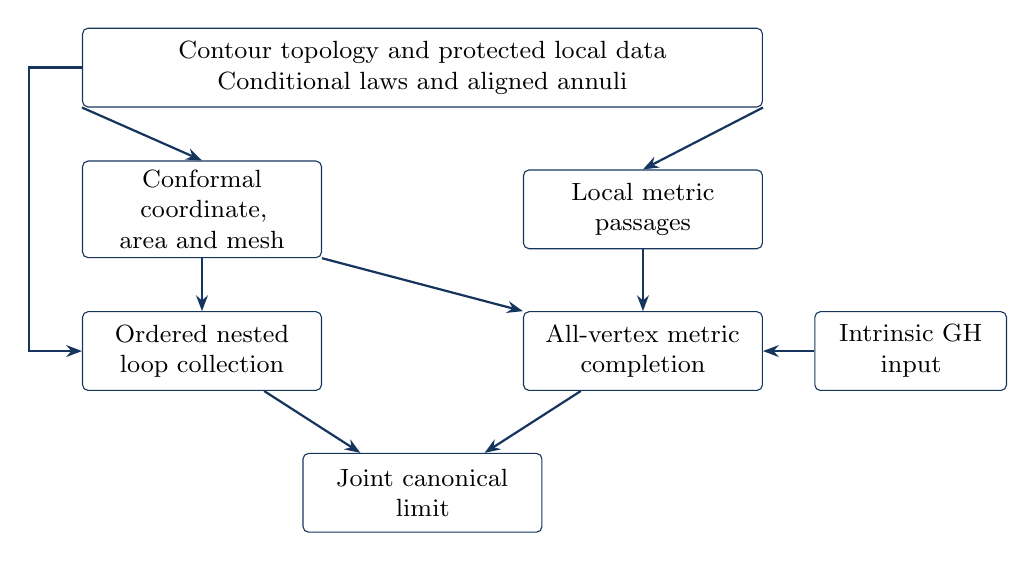
\begin{tikzpicture}[
 box/.style={draw=linkblue,rounded corners=2pt,align=center,
 text width=2.8cm,minimum height=1cm,font=\small},
 arr/.style={-{Stealth[length=2mm]},thick,draw=linkblue},
 node distance=7mm and 9mm]
\node[box,text width=8.4cm] (common) at (0,0)
 {Contour topology and protected local data\\Conditional laws and aligned annuli};
\node[box] (conf) at (-2.8,-1.8) {Conformal coordinate,\\area and mesh};
\node[box] (pass) at (2.8,-1.8) {Local metric\\passages};
\node[box] (loops) at (-2.8,-3.6) {Ordered nested\\loop collection};
\node[box] (comp) at (2.8,-3.6) {All-vertex metric\\completion};
\node[box,text width=2.2cm] (gh) at (6.2,-3.6) {Intrinsic GH\\input};
\node[box] (joint) at (0,-5.4) {Joint canonical\\limit};
\draw[arr] (common.south west)--(conf.north);
\draw[arr] (common.south east)--(pass.north);
\draw[arr] (common.west)--(-5,0)--(-5,-3.6)--(loops.west);
\draw[arr] (conf)--(loops);
\draw[arr] (conf.south east)--(comp.north west);
\draw[arr] (loops)--(joint);
\draw[arr] (pass)--(comp);
\draw[arr] (gh)--(comp);
\draw[arr] (comp)--(joint);
\end{tikzpicture}
\caption{The conformal, loop and metric arguments share the contour
correspondence. The intrinsic GH input enters only the all-vertex
completion of the metric.}
\label{intro:roadmap-figure}
\end{figure}

\section{The model, normalization and topologies}\label{intro:model-section}

\subsection{The finite FK law}

\begin{definition}[Finite ensemble]\label{intro:finite-law}
Let $\mathcal F_n$ consist of pairs $(M,A)$, where $M$ is a connected
planar multigraph with $n$ edges embedded in the oriented sphere and
rooted at a distinguished oriented edge, and $A\subseteq E(M)$.
Pairs are identified under orientation-preserving homeomorphisms
preserving the root and $A$. Loops and multiple edges are allowed.
Let $M^*$ be the dual map, and let $A^*$ consist of the dual edges
crossing $E(M)\setminus A$. Write $k(A)$ and $k(A^*)$ for the numbers
of connected components of the respective spanning subgraphs,
including isolated vertices. Set
\[
 \ell(M,A)=k(A)+k(A^*)-1
         =2k(A)+|A|-|V(M)|,
 \qquad
 Z_n(q)=\sum_{(M,A)\in\mathcal F_n}q^{\ell(M,A)/2}.
\]
We sample $(M_n,A_n)$ with probability
$q^{\ell(M,A)/2}/Z_n(q)$. Its graph distance $d_n$ is shortest-path
distance on $V(M_n)$ using all edges of $M_n$, each of length one.
\end{definition}

For completeness, thicken the vertices and occupied edges to a regular
neighborhood $N(A)$. It has Euler characteristic $|V(M)|-|A|$.
Every component has genus zero. If its total number of boundary
components is $b_A$, then
$|V(M)|-|A|=2k(A)-b_A$, so $b_A=2k(A)+|A|-|V(M)|$.
The complementary components correspond to the components of $A^*$;
Euler's formula on the sphere gives $b_A=k(A)+k(A^*)-1$.
This proves the displayed identities and identifies $\ell$ with the
number of FK interfaces, including configurations containing bridges
or loops.

\subsection{Flag triangles and the fixed conformal coordinate}

For each occurrence of an endpoint and a side of an original edge,
take an equilateral triangle with labels $(v,e,f)$: original vertex,
edge midpoint and face center. Glue sides by their incidence
identifications. There are $4n$ triangles. Repeated incidences are
different occurrences, even when two labels refer to the same vertex,
edge or face. In particular this construction is the incidence
subdivision of the embedded sphere and produces a topological sphere
$X_n$, also for loops and bridges.

The Euclidean metrics on the triangles define a conformal structure
away from their conical vertices. At a cone of total angle $\theta>0$,
the coordinate obtained by raising the local cone coordinate to the
power $2\pi/\theta$ extends this structure across the vertex. Give
$X_n$ normalized Euclidean face area $m_n$, so each triangle has
mass $1/(4n)$. Conditional on $X_n$, take three independent samples
$x_n^1,x_n^2,x_n^3$ from $m_n$. Since $m_n$ has no atoms they are
almost surely distinct. Genus-zero uniformization
\cite[Theorem~II.2.15]{SaintGervais2016Uniformization} and three-point
normalization give a unique orientation-preserving conformal map
\[
 \phi_n:X_n\longrightarrow\Chat,
 \qquad
 \phi_n(x_n^1)=0,\quad\phi_n(x_n^2)=1,\quad
 \phi_n(x_n^3)=\infty.
\]
This is a function of the discrete surface and the three samples.

In a triangle write $(t_v,t_e,t_f)$ for barycentric coordinates.
Include $\{t_v\ge2/3\}$ and, if the original edge belongs to $A_n$,
also include $\{t_f\le1/3\}$. Their glued union is a regular
neighborhood of the occupied primal subgraph. Its boundary components
are the prescribed polygonal interfaces. Write $\widehat\Gamma_n$
for their collection on $X_n$, taken as unrooted and unoriented loops,
and $\Gamma_n=\phi_n(\widehat\Gamma_n)$ for the canonical images.

\begin{lemma}[Flag area and a uniform root]\label{intro:root-flag}
Let $\pi_n$ send the interior of each flag triangle to its primal
vertex, with an arbitrary convention on triangle boundaries. Then
\begin{equation}\label{intro:degree-measure}
 (\pi_n)_*m_n
 =\nu_n:=\frac1{2n}\sum_{v\in V(M_n)}\deg_{M_n}(v)\delta_v.
\end{equation}
Conditional on the unrooted decorated map, the tail of a uniform
oriented root edge has law $\nu_n$, and re-rooting uniformly preserves
the finite decorated law. If $H_n:X_n\to S$ are homeomorphisms into
a compact metric sphere with
$\max_T\diam H_n(T)\to0$, then $(H_n)_*m_n$ and
$(H_n)_*\nu_n$ have the same weak subsequential limits.
\end{lemma}

\begin{proof}
A primal vertex $v$ is incident to $2\deg(v)$ flag occurrences;
a loop contributes twice to $\deg(v)$ and all four of its occurrences
are counted. Thus its mass is $2\deg(v)/(4n)$, proving
\eqref{intro:degree-measure}. There are $2n$ oriented edge
occurrences, and exactly $\deg(v)$ have tail $v$. Uniform re-rooting
preserves the weight $q^{\ell/2}$; equivalently, count rooted
occurrences before quotienting by the automorphism group. This also
proves the assertion in the presence of automorphisms.
Couple $x\sim m_n$ to $\pi_n(x)$. Their $H_n$ images lie in the
same flag image, so their distance is at most
$\max_T\diam H_n(T)$. Testing against uniformly continuous
functions on the compact sphere proves the last assertion.
\end{proof}

The area samples used for $\phi_n$ are fresh independent samples.
\Cref{intro:root-flag} describes the distribution of the forgotten
discrete root; it does not replace those three samples by exploration
marks.

\subsection{The continuum object}

The continuum surface is the ordinary $\gamma$-LQG sphere of
\citet[Definition~4.21(ii)]{DMSMating}, disintegrated at area one. Forget
its original marked points. Given the surface, sample three independent
points from its quantum-area probability measure and send them to
$0,1,\infty$ by an orientation-preserving conformal map. The area
measure is diffuse with full support, so this normalization is almost
surely defined. Write $h$ for a representative field in that
coordinate, $\mu_h$ for its area and $D_h$ for its intrinsic metric.
The metric is a continuous length metric inducing the topology of
$\Chat$. Its deterministic multiplicative normalization remains
fixed.

Given this embedded marked surface, sample the M\"obius-invariant
whole-plane nested $\mathrm{CLE}_{\kappa}$ ensemble on $\Chat$.
This conditional-law specification is part of the joint limit.
The original root and the original quantum-sphere marks are absent
from the limiting object.

\subsection{Distance graphs and loop matching}

Use the product distance
\[
 d_\times((z,w,r),(z',w',r'))
   =\rho(z,z')+\rho(w,w')+|r-r'|
\]
on $\Chat^2\times[0,\infty)$. The distance graphs
$K_n(a)$ in \eqref{intro:distance-graph} are nonempty compact sets.
Since $D_h$ is continuous on the compact sphere, its full graph is
also compact. We use the Hausdorff topology for $d_\times$.

\begin{definition}[Loop and ensemble convergence]
\label{intro:loop-topology}
Our curve distance and locally finite multiset topology follow
\citet[Section~2.2]{GwynneMillerQianCLE}, with loop orientation additionally
forgotten. They retain the order within each loop and its multiplicity.
For continuous loops $\alpha,\beta:\mathbb S^1\to\Chat$, let
\[
 d_{\mathrm{loop}}(\alpha,\beta)
 =\inf_{\sigma}\sup_{t\in\mathbb S^1}
       \rho(\alpha(t),\beta(\sigma(t))),
\]
where $\sigma$ ranges over circle homeomorphisms of either orientation.
Identify loops at zero distance. A loop collection is locally finite
in diameter if it has finitely many loops of diameter greater than
$\varepsilon$ for every $\varepsilon>0$.
An $\varepsilon$-matching of two such collections is a partial
bijection covering every loop of diameter greater than $\varepsilon$
on either side, with matched loops at distance at most $\varepsilon$;
every unmatched loop has diameter at most $\varepsilon$.
Convergence means that such matchings exist with
$\varepsilon\to0$. All collections in this paper retain nested loops.
\end{definition}

This definition also allows repetitions to be retained as separate
elements when forming a matching. The loop identification proof will
establish both local finiteness in diameter and eventual matching of
every macroscopic loop.

\subsection{Extraction conventions}

Let $d_\gamma$ denote the deterministic Hausdorff dimension of the
$\gamma$-LQG metric \citep{GwynneMillerMetric}. We use
$p=1/d_\gamma$, $\xi=\gamma p$, and
$Q=2/\gamma+\gamma/2$. The parameter $q$ always denotes the FK
weight; the inventory parameter is $b$. A crossing scale is denoted
by $B(n)$, whereas $a_n$ denotes the deterministic normalization in
\cref{intro:intrinsic-input}. The exploration root is $p_*$.

All subsequential arguments retain the same contour encoding,
continuum surface, local observations and independent area marks.
Whenever a new finite family of tests is added, refine this joint
extraction. The families used below admit countable determining
atlases: rational time cuts, rational spatial boxes, rational height
slacks and integer truncations. A diagonal refinement therefore
retains all their conclusions on a common event of probability one.
Statements involving all spatial points will be proved by explicit
uniform estimates before passing from an atlas to arbitrary points.

\section{The inventory encoding and its reference surfaces}
\label{enc:section}

The inventory word determines the primal map together with an auxiliary
spanning tree and its complementary dual tree.  Their contours will
provide the reference sphere used in the topological comparison.
We first fix the time and height conventions.  One inventory letter represents
one exploration triangle, which consists of two of the flag triangles
of \Cref{intro:model-section}.  A word of length $2n$ has duration one
after division of time by $2n$.  Multiplying both contour coordinates by one
fixed constant makes their limiting marginal variances one.  This constant is
also used when contour heights are interpreted as quantum boundary lengths.

\subsection{The exact inventory law}

Write $\mathsf h,\mathsf c$ for the two burger types,
$\mathsf H,\mathsf C$ for their rigid orders, and $\mathsf F$ for a flexible
order.  Reading from left to right, an order removes the most recently
produced available burger of an allowed type.  Reduction retains the
unfulfilled orders, in chronological order, followed by the surviving stack.
Set
\begin{equation}\label{enc:letter-law}
 b=\frac{\sqrt q}{2+\sqrt q}\in(0,1/2),\qquad
 \PP(\mathsf h)=\PP(\mathsf c)=\frac14,\quad
 \PP(\mathsf H)=\PP(\mathsf C)=\frac{1-b}{4},\quad
 \PP(\mathsf F)=\frac b2.
\end{equation}
In the bilateral iid word every letter has a unique match almost surely
\cite[Proposition 2.2]{SheffieldInventory}.  Resolve $\mathsf F$ as
$\mathsf H$ or $\mathsf C$ according to its matched burger.  The resolved
contour $Z=(L,R)$ increases by the appropriate coordinate vector at a burger
and decreases by that vector at its order.  It is linearly interpolated
between integer times and anchored at $Z(0)=0$.  Write $N_{\mathsf F}$
for the number of flexible orders in a finite word.

\begin{proposition}[Inventory realization]\label{enc:inventory-law}
The iid word of length $2n$, conditioned to reduce to the empty word,
encodes exactly the rooted FK-decorated map law of the theorem.  Its
underlying primal map, with every primal edge retained, is the map obtained
by the tree/cotree sewing of its resolved contour.  The FK interface count
equals $1+N_{\mathsf F}$.
\end{proposition}

\begin{proof}
The inventory bijection is the rooted map bijection of
\cite[Sections 4.1--4.2]{SheffieldInventory}.  The conversion from a
spanning subgraph to the auxiliary spanning tree is the construction of
\citet[Section~4]{Bernardi2008Subgraphs}, as explained in
\citet[Section~4.1]{SheffieldInventory}.  Its elementary sewing objects
are incidence occurrences, so loops, bridges, and repeated incidences are
included.  A matched burger/order pair forms the two exploration triangles
in one quadrangle.  The $L$-pairs give the primal spanning-tree edges;
the $R$-pairs give the dual spanning-tree edges, whose quadrangles carry the
remaining primal edges.  Resolving a flexible order selects the auxiliary
tree/cotree diagonal.  Restoring its FK diagonal changes the decoration,
not the quadrangle or the underlying all-edge primal map.

A fully matched word has $n$ burgers and $n$ orders.  Its unconditioned
probability is
\[
 \left(\frac{1-b}{16}\right)^n
 \left(\frac{2b}{1-b}\right)^{N_{\mathsf F}}.
\]
The bijection's loop-opening operation gives one initial interface and one
additional interface for each flexible order.  Since
$2b/(1-b)=\sqrt q$, the probability is a constant depending only on $n,q$
times $q^{\#\Gamma/2}$, which is the specified finite map weight.
The rooted bijection is bijective, rather than a quotient weighted by
automorphism counts.  Uniform rerooting at an incidence preserves the law
because every map under consideration has the same number of root
incidences.  These observations also show why deleting cotree-associated
primal edges would change the metric in the theorem.
\end{proof}

\Cref{enc:flag-quadrangle} distinguishes the two exploration triangles
from the four flags of an original edge.  It also records the local
interface pairings determined by the edge's occupation status.

\begin{figure}[ht]
\centering
\begingroup
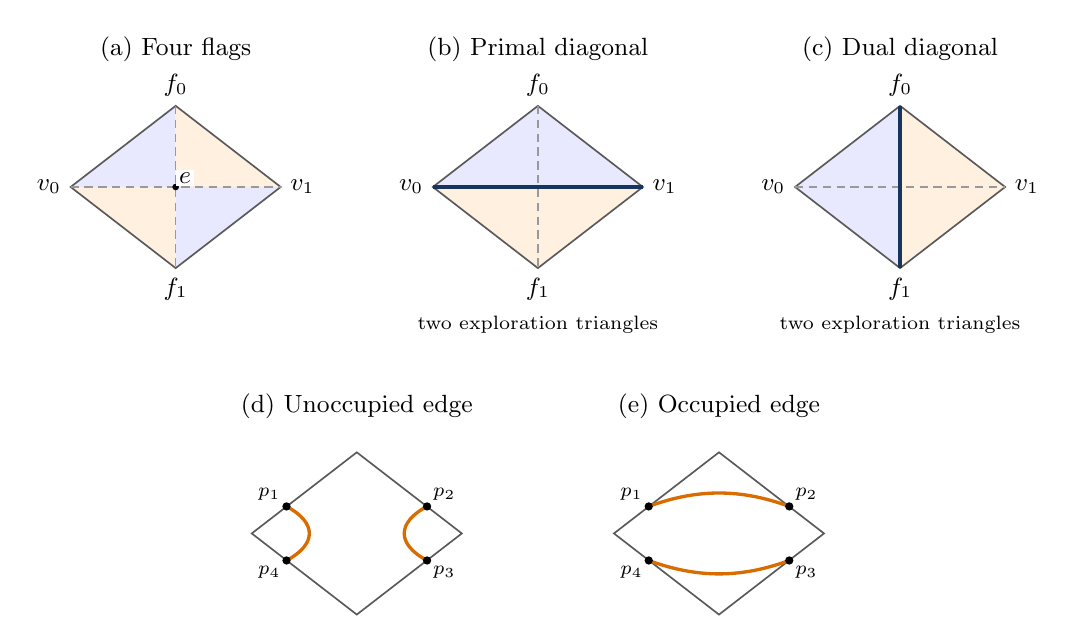
\begin{tikzpicture}[x=.92cm,y=.92cm,font=\small,
  boundary/.style={draw=black!65,line width=.6pt},
  seam/.style={draw=black!40,densely dashed,line width=.45pt},
  diagonal/.style={draw=linkblue,line width=1.2pt},
  interface/.style={draw=orange!85!black,line width=1.2pt}]

\begin{scope}[xshift=0cm]
  \fill[blue!9] (-1.45,0)--(0,1.12)--(0,0)--cycle;
  \fill[orange!12] (0,1.12)--(1.45,0)--(0,0)--cycle;
  \fill[blue!9] (1.45,0)--(0,-1.12)--(0,0)--cycle;
  \fill[orange!12] (0,-1.12)--(-1.45,0)--(0,0)--cycle;
  \draw[boundary] (-1.45,0)--(0,1.12)--(1.45,0)--(0,-1.12)--cycle;
  \draw[seam] (-1.45,0)--(1.45,0) (0,1.12)--(0,-1.12);
  \node[left] at (-1.45,0) {$v_0$};
  \node[right] at (1.45,0) {$v_1$};
  \node[above] at (0,1.12) {$f_0$};
  \node[below] at (0,-1.12) {$f_1$};
  \fill (0,0) circle (1.2pt);
  \node[fill=white,inner sep=1pt,above right] at (0,0) {$e$};
  \node at (0,1.90) {(a) Four flags};
\end{scope}

\begin{scope}[xshift=4.6cm]
  \fill[blue!9] (-1.45,0)--(0,1.12)--(1.45,0)--cycle;
  \fill[orange!12] (-1.45,0)--(0,-1.12)--(1.45,0)--cycle;
  \draw[boundary] (-1.45,0)--(0,1.12)--(1.45,0)--(0,-1.12)--cycle;
  \draw[seam] (0,1.12)--(0,-1.12);
  \draw[diagonal] (-1.45,0)--(1.45,0);
  \node[left] at (-1.45,0) {$v_0$};
  \node[right] at (1.45,0) {$v_1$};
  \node[above] at (0,1.12) {$f_0$};
  \node[below] at (0,-1.12) {$f_1$};
  \node at (0,1.90) {(b) Primal diagonal};
  \node[font=\scriptsize] at (0,-1.90) {two exploration triangles};
\end{scope}

\begin{scope}[xshift=9.2cm]
  \fill[blue!9] (-1.45,0)--(0,1.12)--(0,-1.12)--cycle;
  \fill[orange!12] (1.45,0)--(0,1.12)--(0,-1.12)--cycle;
  \draw[boundary] (-1.45,0)--(0,1.12)--(1.45,0)--(0,-1.12)--cycle;
  \draw[seam] (-1.45,0)--(1.45,0);
  \draw[diagonal] (0,1.12)--(0,-1.12);
  \node[left] at (-1.45,0) {$v_0$};
  \node[right] at (1.45,0) {$v_1$};
  \node[above] at (0,1.12) {$f_0$};
  \node[below] at (0,-1.12) {$f_1$};
  \node at (0,1.90) {(c) Dual diagonal};
  \node[font=\scriptsize] at (0,-1.90) {two exploration triangles};
\end{scope}

\begin{scope}[xshift=2.3cm,yshift=-4.4cm]
  \draw[boundary] (-1.45,0)--(0,1.12)--(1.45,0)--(0,-1.12)--cycle;
  \draw[interface] (-.97,.373) .. controls (-.55,.15) and (-.55,-.15) .. (-.97,-.373);
  \draw[interface] (.97,.373) .. controls (.55,.15) and (.55,-.15) .. (.97,-.373);
  \foreach \x/\y/\lab/\pos in {-.97/.373/1/above left,.97/.373/2/above right,.97/-.373/3/below right,-.97/-.373/4/below left}{
    \fill (\x,\y) circle (1.5pt);
    \node[\pos,inner sep=2pt,font=\scriptsize] at (\x,\y) {$p_{\lab}$};
  }
  \node at (0,1.75) {(d) Unoccupied edge};
\end{scope}

\begin{scope}[xshift=6.9cm,yshift=-4.4cm]
  \draw[boundary] (-1.45,0)--(0,1.12)--(1.45,0)--(0,-1.12)--cycle;
  \draw[interface] (-.97,.373) .. controls (-.3,.62) and (.3,.62) .. (.97,.373);
  \draw[interface] (-.97,-.373) .. controls (-.3,-.62) and (.3,-.62) .. (.97,-.373);
  \foreach \x/\y/\lab/\pos in {-.97/.373/1/above left,.97/.373/2/above right,.97/-.373/3/below right,-.97/-.373/4/below left}{
    \fill (\x,\y) circle (1.5pt);
    \node[\pos,inner sep=2pt,font=\scriptsize] at (\x,\y) {$p_{\lab}$};
  }
  \node at (0,1.75) {(e) Occupied edge};
\end{scope}
\end{tikzpicture}
\endgroup

\caption{Incidences at one original edge.  The four flags have labels
$(v_i,e,f_j)$, $i,j\in\{0,1\}$.  Selecting the primal or dual auxiliary
diagonal groups them into the two exploration triangles of the matched
letters.  The lower panels show the two pairings of the four interface
ports: an unoccupied edge pairs ports about each primal endpoint,
whereas an occupied edge pairs them about each incident face.
This is a topological schematic, not an isometric drawing of the
equilateral flags.  Labels may repeat for a loop or bridge, but the
four flag and port occurrences remain distinct.}
\label{enc:flag-quadrangle}
\end{figure}

\begin{lemma}[Tree and incidence identities]\label{enc:incidence}
For a fully matched resolved word, let $T_n$ be its primal spanning tree
and $T_n^*$ the complementary dual spanning tree.  At the cut after
letter $k$, the exploration has a primal corner vertex $v_n(k)$ and a
dual corner face $f_n(k)$.  In unscaled integer height units,
\begin{align*}
 d_{T_n}(v_n(k),v_n(l))
 &=L_k+L_l-2\min_{j\in[k,l]}L_j,\\
 d_{T_n^*}(f_n(k),f_n(l))
 &=R_k+R_l-2\min_{j\in[k,l]}R_j,
 \qquad 0\le k\le l\le2n.
\end{align*}
Every primal vertex and dual face occurrence is represented by these
corner sequences.  Each quadrangle is the union of its two matched
exploration triangles; each such triangle is incident to the corner
states immediately before and after its letter.  Thus the endpoints,
faces, and flag incidences of a quadrangle have a uniformly bounded
collection of tour representatives.  The representatives for each
primal vertex are identified by the $L$-tree rule, and those for each
dual vertex by the $R$-tree rule; moving from a cut to its adjacent
triangle changes a height by at most one.
\end{lemma}

\begin{proof}
After resolution this is the ordinary tree/cotree contour exploration
in \cite[Section 4.1, Figures 6--7]{SheffieldInventory}.  A burger
creates an edge to a child in its tree and its order returns along
that edge.  Letters of the other type hold this tree position fixed.
The depth of the common ancestor of the positions at $k,l$ is the
minimum contour height between them, proving the two distance
identities.  The exploration crosses each tree-edge side and each
quadrangle side occurrence, which proves coverage of the corners,
including repeated occurrences.  A letter triangle is bounded by the
two successive exploration sides and the created or traversed tree
edge.  Pairing it with its matching letter triangle gives exactly the
associated quadrangle.  Subdivision into flags introduces an edge
midpoint but no additional incidence choice.  This proves the last
assertions without any bound on vertex or face degrees.
\end{proof}

\begin{theorem}[Contour limits]\label{enc:contour-limits}
Let
\[
 \varrho=\frac b{1-b}=-\cos\left(\frac{\pi\gamma^2}{4}\right),
 \qquad \gamma\in(\sqrt2,2),\qquad \kappa=\frac{16}{\gamma^2}.
\]
The diffusively rescaled bilateral resolved contours converge, uniformly
on compact time intervals in law, to a bilateral Brownian motion whose
marginal variance rates are one and whose correlation is $\varrho$.
For a length-$2n$ word conditioned to reduce to the empty word, the same
rescaling, with duration one, converges uniformly in law to the corresponding
quadrant Brownian excursion from $(0,0)$ to $(0,0)$.

For an unconditioned raw block of $O(n)$ letters, the number of flexible
orders left unidentified by reduction of the block is $o_{\PP}(\sqrt n)$.
Consequently changing their resolutions changes the rescaled contour
increments by $o_{\PP}(1)$ uniformly on that block.
\end{theorem}

\begin{proof}
The bilateral assertion is \cite[Theorem 2.5]{SheffieldInventory}.
In the original units the covariance rates of the two net burger counts
are $(1-b)/2,(1-b)/2,b/2$; multiplying heights by
$\sqrt{2/(1-b)}$ gives the stated convention.  The conditioned assertion is
\cite[Theorem 1.8]{GwynneSunFKIII}, followed by the deterministic change
from duration two to duration one.  The unidentified-order estimate is
\cite[Remark 3.17]{SheffieldInventory}; see also the reduced-word estimates
in \cite{GwynneMaoSunFKI}.  Each changed resolution changes a contour
coordinate by at most one, so their total number bounds the supremum error.
This last assertion concerns a raw unconditioned block.  The transfer of
discrete observations to conditioned extractions will be proved in
Section~\ref{ker:section}.
\end{proof}

\subsection{The reference LQG surfaces}

\begin{theorem}[Peanosphere realization]\label{enc:peanosphere}
The bilateral Brownian contour is the boundary-length process of a
$\gamma$-quantum cone explored by an independent, unparameterized
whole-plane space-filling $\mathrm{SLE}_{\kappa}$, subsequently
parameterized by quantum area.  The duration-one excursion is the
boundary-length process of the ordinary unit-area $\gamma$-quantum sphere
explored in the same way from an area-typical marked point $p_*$.
The contour determines the curve-decorated quantum surface up to its
marked conformal equivalence.

Write $\eta$ for the exploration parameterized by quantum area.
In either realization, $\eta_*(\dd t)=\mu_h$.  Its spatial identifications
are generated by finite chains of scalar horizontal chords
\begin{equation}\label{enc:chord-rule}
 s\sim_L t\quad\Longleftrightarrow\quad
 L_s=L_t=\inf_{[s,t]}L,
 \qquad s<t,
\end{equation}
and the analogous $R$-chords, with the usual endpoint identification for
the sphere.  The resulting quotient carries the topology of the plane,
or sphere, respectively.  Frontier arcs are parameterized by quantum
length, with running-minimum contour heights as their length coordinates.
\end{theorem}

\begin{proof}
For the cone, the surface and contour identification are the
mating-of-trees and welding theorems
\cite[Theorems~1.9 and~1.11]{DMSMating}. For the ordinary area-one sphere,
\cite[Theorem~1.1]{MillerSheffieldSphere} supplies the Brownian-loop law
and determination of the surface explored by an independent unclocked
whole-plane space-filling SLE. In our range $\gamma^2\in(2,4)$ the
covariance is the one in these theorems. The marked-point sampling rule
is \cite[Proposition~A.13]{DMSMating}. We use the common deterministic
boundary-length convention specified above, with area-clock duration one.

Call a scalar chord \emph{strict} if the contour is strictly above its
endpoint height between the endpoints.  The finite-chain assertion uses
a further geometric part of the DMS
construction. There are finitely many visits to each spatial point;
ordering their left and right flow-line sectors links consecutive visits
by scalar chords. This is the smallest generated equivalence relation in
\cite[Lemmas~8.9, 8.13--8.15 and Theorem~8.18]{DMSMating}, without taking
its closure. A non-strict scalar chord can be split at its possible
intermediate minimum visit into adjacent strict chords; scalar fibers
have at most three visits. The same finite-visit and adjacent-sector
argument applies to the independent whole-plane exploration of the
sphere away from its exploration root: changing to quantum-area time
preserves the visits, their order and their frontier incidences. At the
root one additionally identifies $0$ and $1$. Thus the sphere statement
combines its Brownian-loop realization with this geometric argument;
it does not invoke a separately stated sphere finite-chain theorem.
The quotient is topological because the resulting continuous bijection
from the compact time quotient to the sphere is a homeomorphism.
Running-minimum frontier coordinates are the quantum lengths supplied
by the same welding construction.
\end{proof}

We use actual field heights when comparing passage laws.  The following
description records explicitly the area normalization that couples
different patches.

\begin{proposition}[Three-mark sphere representation]
\label{enc:sphere-representation}
Let $h_{\C}$ be the whole-plane Gaussian free field (GFF) with circle average zero on
$\partial\mathbb D$, and put
\[
 |z|_+=\max\{1,|z|\},\qquad
 G_{\C}(z,w)=\log\frac{|z|_+|w|_+}{|z-w|},\qquad
 Q=\frac2\gamma+\frac\gamma2.
\]
Define
\begin{equation}\label{enc:liouville-field}
 h_L=h_{\C}+\gamma G_{\C}(0,\cdot)+\gamma G_{\C}(1,\cdot)
       -(2Q-\gamma)\log|\cdot|_+,
 \quad A=\mu_{h_L}(\C).
\end{equation}
Tilt the law of $h_L$ by the integrable strictly positive density
$A^{4/\gamma^2-2}/\EE[A^{4/\gamma^2-2}]$, and then set
\begin{equation}\label{enc:area-normalization}
 h=h_L-\gamma^{-1}\log A.
\end{equation}
The result is the ordinary unit-area sphere with three independent
area marks embedded at $\infty,0,1$.  Resampling its three area marks and
renormalizing gives the same law.  In particular, on any bounded region
avoiding $0,1$, its field modulo constants is locally mutually absolutely
continuous with a whole-plane GFF modulo constants.  Near $0$, away from
$1$, the corresponding comparison field is $h_{\C}-\gamma\log|\cdot|$.
\end{proposition}

\begin{proof}
This fixed-area field law originates in the sphere construction of
David, Kupiainen, Rhodes and Vargas
\citep[Section~3.3, Proposition~3.8 and Section~3.4]{DKRVSphere2016}.
We use its form in \citet[Definition~2.2]{BorgaGwynneSunPermutons};
\citet[Theorem~1.1 and Remark~1.2]{AruHuangSunSphere} identify it with
the ordinary DMS sphere.
The mark resampling statement and local comparison, including the
$\gamma$-insertion, are \cite[Lemmas 2.3--2.4]{BorgaGwynneSunPermutons}.
Subtracting the constant in \eqref{enc:area-normalization} gives area one
by the identity $\mu_{h+c}=e^{\gamma c}\mu_h$.
\end{proof}

The proposition deliberately retains the common random constant
$-\gamma^{-1}\log A$.  Local equivalence modulo constants alone does not
give a joint law for actual heights in several patches.  The required
joint density is derived from \eqref{enc:liouville-field}--
\eqref{enc:area-normalization} in Section~\ref{ker:section}.

\section{A topological correspondence for every flag}
\label{top:section}

Contour convergence initially relates exploration times.  We need a
correspondence on the whole discrete surface which preserves separation
and intersections.  This section constructs it without estimating the
length of any connecting walk.  Throughout the finite-volume argument we
work on a coupling on which the contours converge uniformly, write
$Z_n=(L_n,R_n)$ for the rescaled contours, and write
$\eta:[0,1]\to S$ for the limiting exploration.  Equip the reference
topological sphere $S$ with a fixed spherical metric $\rho$ in any of its
conformal coordinates.  The choice of this coordinate is immaterial to
the deterministic assertions below.

\subsection{Scalar trees and the continuous projection}

For a continuous real function $c$ on a compact time interval, put
\begin{equation}\label{top:tree-pseudometric}
 d_c(s,t)=c(s)+c(t)-2\min_{[s\wedge t,s\vee t]}c.
\end{equation}
The equivalence classes for $d_c=0$ are the vertices of its contour tree.
We use the exact primal-tree and dual-tree incidence description in
Lemma~\ref{enc:incidence}.  Heights of a discrete tree edge in this
section have the same rescaled units as $L_n,R_n$; its graph length is
still one whenever graph costs are subsequently considered.

\begin{lemma}[Continuity of the scalar trees]\label{top:scalar-trees}
If $c_n\to c$ uniformly, then
\[
 \sup_{s,t}|d_{c_n}(s,t)-d_c(s,t)|
 \le 4\|c_n-c\|_\infty.
\]
Suppose $s_n\to s$, $t_n\to t$, and $d_c(s,t)=0$.
Every contour representative of every vertex on the discrete
$c_n$-tree path between the vertices at $s_n,t_n$ has distance
$d_{c_n}$ tending to zero from the vertex at $s_n$, uniformly over those
representatives.  Consequently, if $c$ is $L$ or $R$, their images under
$\eta$ tend uniformly to $\eta(s)$.

For $c_n=R_n$, take the faces represented by the vertices of this
dual-tree path.  The union of their primal boundary walks is a connected
primal subgraph.  All its corner representatives have $\eta$-images
tending uniformly to $\eta(s)$.
\end{lemma}

\begin{proof}
The displayed inequality follows by bounding the two endpoint errors and
the error of the minimum.  A vertex $u$ on a tree geodesic from $a$ to $b$
satisfies $d(a,u)\le d(a,b)$.  The exact contour-tree identity therefore
bounds all the asserted distances by
$d_{c_n}(s_n,t_n)$, up to one rescaled edge if a cut lies inside a step.
This tends to zero.  If the assertion about $\eta$ were false, choose a
representative $u_n$ violating it and then a convergent subsequence of
$u_n$.  Its limit $u$ satisfies $d_c(s,u)=0$, so
$\eta(u)=\eta(s)$ by the scalar chord rule, contradicting continuity of
$\eta$.

Consecutive faces of a dual-tree path share the primal edge crossed by
that tree edge.  Their entire boundary walks therefore have connected
union, including when a boundary edge or vertex is visited repeatedly.
A corner of any of these faces represents its dual-tree vertex, so the
same distance bound applies to all its representatives.  This proves
the last assertion.  No bound on a face degree is involved.
\end{proof}

The tour supplies finitely many time representatives for each flag
incidence, as specified in Lemma~\ref{enc:incidence}.  We may use
either endpoint of an exploration step; changing that choice changes the
time by at most one mesh interval.  A representative of a primal vertex
means any tour occurrence of that vertex, and similarly for a dual
vertex.  The occurrences at a loop or bridge remain distinct.

\begin{proposition}[Projection of the complete flag surface]
\label{top:projection}
There are continuous maps $P_n:X_n\to S$ and numbers
$\varepsilon_n\to0$ such that the following hold simultaneously.
\begin{enumerate}[label=(\roman*)]
\item For every flag $T$, every $x\in T$, and every tour representative
associated to any of the corners of its quadrangle,
\[
 \rho(P_n(x),\eta(t))\le\varepsilon_n.
\]
The same conclusion holds for any other occurrence of an incident primal
or dual vertex.
\item The $P_n$-images of individual flags, original edges, original
closed faces, and complete primal or dual incidence stars have maximum
diameter tending to zero.
\item The sets $P_n(V(M_n))$ become dense in $S$.
\end{enumerate}
These conclusions hold for the original flag complex, with all repeated
incidence occurrences retained.
\end{proposition}

\begin{proof}
First choose one representative for every primal vertex and every dual
vertex.  Representatives of a given primal vertex have zero
$L_n$-tree distance; representatives of a given dual vertex have zero
$R_n$-tree distance.  Uniform contour convergence, compactness of the
time interval, and the chord rule show that the maximum disagreement
between their $\eta$-images tends to zero.  This is a uniform statement:
a failing sequence of vertices and two of their occurrences would have
convergent time representatives and would contradict the limiting chord
rule.

At a tour cut the primal and dual corner states have that same time
representative.  In one quadrangle its four corner states are linked
successively by equality of a primal or a dual vertex, together with the
two consecutive-cut errors of its exploration triangles.  The preceding
uniform assertion and continuity of $\eta$ show that all these
representatives agree up to a uniform error tending to zero.  It follows
that the chosen representatives of the primal vertex and face center
of every flag agree to this accuracy.  Assign its edge midpoint the
image of one fixed corner occurrence of that edge.  The preceding
quadrangle argument gives the same conclusion for this assignment.

Identify $S$ with the unit sphere in $\R^3$.  On every flag send a point
with barycentric coordinates $(a_1,a_2,a_3)$ to
\[
 \frac{a_1 y_1+a_2 y_2+a_3 y_3}
 {|a_1 y_1+a_2 y_2+a_3 y_3|},
\]
where $y_1,y_2,y_3$ are the assigned images of its vertices.  For all
large $n$ the three images lie in a common ball of radius less than
$\pi/4$, so the denominator is nonzero.  These formulas agree on glued
sides and give a continuous map on the flag quotient.  Their images
stay in the same small spherical ball.  This proves (i) and the flag
assertion in (ii).  Every flag in a primal or dual star shares the
image of its central vertex, so its entire star has diameter at most
twice the maximum flag diameter.  The assertions for edges and faces
follow as well.  Finally the tour meshes become dense in $[0,1]$,
$\eta$ is onto, and every tour position has a primal corner vertex
with the stated small error.  This proves (iii).
\end{proof}

\begin{lemma}[Protection by complete time preimages]
\label{top:protection}
Let $K\subset U\subset S$, where $K$ is compact and $U$ is open.
There are a neighborhood $K'$ of $K$ with $\overline{K'}\subset U$ and a
finite union $I$ of open time intervals such that
\begin{equation}\label{top:time-protection}
 \eta^{-1}(\overline{K'})\subset I,
 \qquad \overline I\subset\eta^{-1}(U).
\end{equation}
Intervals are interpreted on the time circle when necessary.  If
$p_*\notin\overline U$, they are strict subintervals of $(0,1)$.
For all large $n$, every flag whose projection meets $K$, and the full
incidence stars of its three vertices, have all their tour
representatives in $I$.

In the bilateral setting the same assertion holds for bounded compact
spatial protections, with finitely many bounded time intervals.
\end{lemma}

\begin{proof}
Choose two successive compact neighborhoods of $K$ in $U$.
The inverse image of the smaller closed neighborhood is compact and
lies inside the open inverse image of the larger one.  Cover it by
finitely many intervals whose closures lie in that open inverse image.
This proves \eqref{top:time-protection}.  If a sequence of omitted tour
representatives belonged to stars of flags meeting $K$,
Proposition~\ref{top:projection} would force their $\eta$-images into
an arbitrarily small neighborhood of $K$.  They would eventually lie
in $\eta^{-1}(\overline{K'})\subset I$, a contradiction.  Avoiding
$p_*$ keeps the inverse images away from $0,1$.
In the plane, transience of $\eta$ makes the inverse image of every
compact set compact; the same finite-cover proof then applies.
\end{proof}

\subsection{Joining arbitrary lifts with spatial clearance}

\begin{lemma}[Local joining]\label{top:local-joining}
For every $\epsilon>0$ there are $\delta>0$ and $n_0$ such that, for
$n\ge n_0$, $x\in S$, and primal vertices $u,v$ satisfying
\[
 P_n(u),P_n(v)\in B_\rho(x,\delta),
\]
there is a primal graph walk from $u$ to $v$ whose entire projection is
contained in $B_\rho(x,\epsilon)$.
The analogous assertion holds for arbitrary prescribed points of
$X_n$, using continuous paths.  The choice is uniform over the
prescribed lifts.  Its conclusion makes no assertion about the number
of edges in the walk.
\end{lemma}

\begin{proof}
First suppose that representatives $s_n,t_n$ of $u_n,v_n$ converge to
$s,t$ with $s\sim_L t$.  The primal-tree path joins these vertices and
has image tending to the single point $\eta(s)$ by
Lemma~\ref{top:scalar-trees} and Proposition~\ref{top:projection}.
If instead $s\sim_R t$, join the incident dual vertices by their
dual-tree path.  The union of the primal boundaries of its faces is
connected, contains both primal corner vertices, and has the same
vanishing image diameter.  A walk in this connected subgraph supplies
the required primal connection.

For arbitrary $s,t$ with $\eta(s)=\eta(t)$, choose a finite chain of
$L$- and $R$-chords joining them, using
Theorem~\ref{enc:peanosphere}.  For each intermediate time choose its
nearest discrete cut and its primal corner vertex.  The preceding
construction for each link gives finitely many walks whose union tends
to $\eta(s)$; concatenate them.

If the uniform assertion failed, there would be $n_j\to\infty$,
$\delta_j\downarrow0$, points $x_j$, and two prescribed vertices
with images in $B(x_j,\delta_j)$ admitting no walk in
$B(x_j,\epsilon)$.  Choose time representatives and pass to convergent
subsequences $x_j\to x$, $s_j\to s$, $t_j\to t$.
Proposition~\ref{top:projection} gives
$\eta(s)=\eta(t)=x$.  The finite-chain construction just proved
produces the forbidden walks.  For an arbitrary point of a flag, first
join it inside that flag to its primal vertex.  The extra pieces have
vanishing projected diameter by Proposition~\ref{top:projection}.
\end{proof}

To specify an ordered following test for a path $c:[0,1]\to S$,
choose $0=t_0<\cdots<t_r=1$, open ports $U_j$ containing $c(t_j)$,
and open tubes $V_j$ containing $c([t_{j-1},t_j])$.
A follower visits these ports in order, with its intervening pieces
in the corresponding tubes.  The compact reference pieces and the
chosen smaller port neighborhoods have positive clearance inside
these open sets.  A port specifies a visit; a transverse crossing
will require the additional side and clearance conditions below.

\begin{corollary}[Following a finite collection of paths]
\label{top:path-lifting}
Let $c_1,\ldots,c_m$ be continuous paths on $S$ and let prescribed
lifts of their endpoints have the corresponding projected limits.
For every finite ordered following test as above, all sufficiently
large $n$ admit lifted paths whose projections satisfy that test.
Primal endpoint lifts admit
primal walks.  Endpoints which coincide in the reference collection
may be assigned one common prescribed lift.
\end{corollary}

\begin{proof}
Apply Lemma~\ref{top:local-joining} with a spatial error smaller than
the clearance of the chosen finite requirements.  Uniform continuity
gives a finite time partition for each $c_i$ on whose pieces its
oscillation is smaller than the resulting $\delta/3$.  Choose primal
representatives near the partition points using
Proposition~\ref{top:projection}(iii), retaining the prescribed endpoints.
Join successive representatives by the lemma.  Subdivide at the
intermediate ports before making these choices.  Concatenation proves
the ordered assertion, and the same construction works for all the
finitely many paths at once.
\end{proof}

\subsection{From local joining to sphere homeomorphisms}

Local joining initially supplies connected branch sets, rather than
disjoint arcs meeting only at their endpoints.  We use a cubic
skeleton because a minimal tree joining three attachments has just
one trivalent junction after its outgoing paths are attached.
Pruning therefore turns the branch sets into a subdivision, to which
Whitney's embedding theorem and disk extension can be applied.

\begin{lemma}[Lifting a cubic skeleton]\label{top:skeleton-lift}
Let $G\subset S$ be an embedded finite simple cubic graph with
piecewise smooth edges.  For every $\epsilon>0$, all sufficiently large
$n$ contain a primal subgraph $G_n$ which is a subdivision of $G$, and
there is a graph homeomorphism $h_n:G_n\to G$ such that
\[
 \sup_{x\in G_n}\rho(P_n(x),h_n(x))<\epsilon.
\]
If $G$ is $3$-connected, its facial cycles and those of $G_n$ correspond
under this homeomorphism, up to one common reversal of orientation.
\end{lemma}

\begin{proof}
Take pairwise disjoint small closed junction disks about the vertices
of $G$.  In each disk its three incident edges are three disjoint stubs
except for their common endpoint.  Choose three further intermediate
points on the stubs, and narrow disjoint ribbons along the remaining
edge portions.  The ribbons of different edges are disjoint outside
the junction disks.  Inside a junction disk, choose the three ribbon
ends disjoint, so each meets only its own stub neighborhood.  Make
all these neighborhoods small enough for the desired error.

Assign one primal lift to every graph vertex.  By
Corollary~\ref{top:path-lifting}, lift its three initial stubs from
that common lift to the three intermediate points.  Their union is a
connected branch set $B_v$ within the chosen junction neighborhood.
The branch sets belonging to distinct vertices are disjoint, since
their projected neighborhoods are disjoint.  Lift each remaining
edge portion between the corresponding stub endpoints.  The error
may be chosen so small that different connecting walks can intersect
only within branch sets at a common endpoint, and no connecting walk
meets any other branch set.  In particular, near a junction each
connector meets only the end of its own stub; all such contacts occur
before the prescribed marks delimiting the middle of that connector.

For an edge $vw$, take the portion from its last visit to $B_v$
before its first subsequent visit to $B_w$.  Erase loops from that
finite walk.  The resulting simple paths have interiors disjoint
from every branch set and from each other.  At a branch set retain
a minimal finite tree joining its three attachment points.  After
the three outgoing paths are attached, this tree has exactly one
vertex of degree three and every other vertex of degree two; this
also covers coincident attachment points and the case where one
attachment lies between the other two.  Removing unused branches
therefore gives an actual subdivision of $G$.  The use of three
attachments is the reason for choosing a cubic skeleton.

Here is the order control needed to define $h_n$.  Give each edge
ribbon a continuous longitudinal coordinate, equal to its edge
parameter on the central arc.  In the path-lifting construction use
successive coordinate intervals of length less than $\sigma$, and
choose the spatial errors so that each joining piece stays within
$\sigma$ of its prescribed interval.  If a loop-erasure removes a
portion between two occurrences of one vertex, the two original
parameters differ by at most $3\sigma$: their common projected
point has a single longitudinal coordinate within the required
error of both.  Truncation at the branch sets changes only the
initial or final stub.  Assign increasing central-arc parameters to
the surviving vertices, and interpolate strictly increasingly
along the surviving edges.  The skipped parameter intervals have
oscillation tending to zero as $\sigma\downarrow0$.
Within a junction neighborhood map the three remaining tree arms
to the three initial edge pieces.  This gives a graph homeomorphism
whose error is bounded by the ribbon widths, junction diameters,
and those vanishing oscillations.  Choose them in that order to
make the total error smaller than $\epsilon$.

Finally a subdivision induces the same embedding of the suppressed
graph.  Whitney's theorem says that two embeddings of a finite
simple $3$-connected planar graph in the sphere are equivalent up
to a sphere homeomorphism \cite{Whitney1932}.  Its hypotheses hold
for $G$, and hence the identified facial cycles agree, with at most
one global orientation reversal.
\end{proof}

\begin{theorem}[Homeomorphisms with vanishing projection error]
\label{top:homeomorphism}
There are sphere homeomorphisms $H_n:X_n\to S$ such that
\begin{equation}\label{top:homeomorphism-error}
 \sup_{x\in X_n}\rho(H_n(x),P_n(x))\longrightarrow0.
\end{equation}
In particular,
\begin{equation}\label{top:homeomorphism-mesh}
 \max_{T}\diam_\rho H_n(T)\longrightarrow0,
\end{equation}
and the images under $H_n$ of every flag and all its tour
representatives have vanishing maximum disagreement.  The maps may
preserve or reverse orientation, with a common sign on each sphere.
They may be chosen measurably in the contour coupling.  The assertion
continues to hold when that coupling retains any additional random
observations.
\end{theorem}

\begin{proof}
Fix a small $\epsilon>0$.  Triangulate the reference sphere with
simplicial triangles of diameter less than $\epsilon/10$, and take
its embedded dual graph $G$.  Draw dual edges through adjacent
triangle interiors.  Its faces lie in stars of the original vertices,
so their diameters are less than $\epsilon$.
This graph is cubic and $3$-connected.  For the latter assertion,
delete any two dual vertices, or equivalently the corresponding
two closed triangles.  Their union has connected complement in
the sphere, whether the triangles are disjoint, meet at a vertex,
or share an edge.  A path in that complement between two remaining
triangle interiors can be perturbed away from triangulation
vertices; the triangles it successively crosses give a dual path
avoiding the two deleted vertices.  Thus deleting fewer than three
dual vertices does not disconnect the dual graph.  The simplicial
condition also ensures that the dual has neither loops nor multiple
edges.

Apply Lemma~\ref{top:skeleton-lift} with an error much smaller than
$\epsilon$.  Denote by $F_n$ the face of $G_n$ corresponding to a
face $F$ of $G$.  Choose $z_F$ so that
$\overline F\subset B(z_F,\epsilon)$.  We claim that, for all
large $n$,
\begin{equation}\label{top:small-faces}
 P_n(\overline{F_n})\subset B(z_F,3\epsilon).
\end{equation}
The boundaries already satisfy this assertion by the graph
homeomorphism estimate.  If the claim fails in the interiors,
pass to a sequence $x_n\in F_n$ with
$P_n(x_n)\to y\notin B(z_F,3\epsilon)$.  Choose a vertex $v$ of
$G$ outside $B(z_F,3\epsilon)$; such a vertex exists for sufficiently
small $\epsilon$, because the dual graph has small faces and covers
the sphere.  The complement of
$\overline B(z_F,2\epsilon)$ is connected, so join $y$ to $v$ by
a path with clearance from $B(z_F,3\epsilon/2)$.  Lift this path
from the prescribed point $x_n$ to the junction lift of $v$, using
Corollary~\ref{top:path-lifting}.  Its projection avoids
$B(z_F,3\epsilon/2)$ for all large $n$, whereas the projection of
$\partial F_n$ is contained in that ball.  The lifted path
therefore avoids $\partial F_n$.  Its last point is outside
$\overline{F_n}$, since $v$ is not incident to the corresponding
face.  This contradicts the Jordan separation of $\partial F_n$.
There are finitely many faces, so \eqref{top:small-faces} holds
for all of them simultaneously.

Each face of a $3$-connected sphere embedding is a Jordan disk.
The graph homeomorphism $h_n$ therefore extends across every face
to a homeomorphism $H_{n,\epsilon}:X_n\to S$.
For completeness, a homeomorphism between the boundary circles of
two closed disks extends by identifying each disk with the standard
closed disk and extending the resulting circle homeomorphism
radially.  The Jordan--Sch\"onflies theorem gives these disk
identifications; here all boundaries are finite polygonal curves
in triangulated surfaces.  The facial correspondence makes the
extensions agree on common edges.  For $x\in\overline{F_n}$,
both $H_{n,\epsilon}(x)\in\overline F$ and
$P_n(x)\in B(z_F,3\epsilon)$, and hence
\[
 \sup_{x\in X_n}\rho(H_{n,\epsilon}(x),P_n(x))
 \le 4\epsilon.
\]

Take $\epsilon_k\downarrow0$.  At each $k$ the construction works
eventually; increase its threshold $n_k$ so that the thresholds are
strictly increasing, and use $H_{n,\epsilon_k}$ for
$n_k\le n<n_{k+1}$.  This proves
\eqref{top:homeomorphism-error}.  Equation~\eqref{top:homeomorphism-mesh}
follows from Proposition~\ref{top:projection} and the triangle
inequality.

All finite walk choices can be made first in a fixed enumeration.
The graph and its disk extensions can likewise be chosen among
piecewise linear maps after finite subdivisions, with rational
coordinates in fixed spherical charts.  These form a countable
collection; the polygonal disk construction and an arbitrarily
small perturbation give a member satisfying any strictly weakened
error bound above.  Choose the first such member.  Its uniform
error is measurable by taking a supremum over a countable dense
set in each flag.  Choosing the largest available accuracy among
the first $n$ accuracies gives a measurable version of the
diagonal construction.  Finally, the whole argument is
deterministic on the event of contour convergence and the
peanosphere assertions, so retaining other observations does not
alter it.
\end{proof}

\subsection{Protected bilateral windows}

The analogous plane statement is local.  In particular, it does not
require a conformal uniformization of an infinite discrete map, or the
assertion that an arbitrarily capped limiting contour has a sphere
quotient.

\begin{proposition}[Closing a protected window]
\label{top:protected-window}
Work in a bilateral contour coupling with locally uniform convergence
to its peanosphere contour.  Given finitely many compact spatial
tests and open buffers about them, one may choose a bounded time
window, and then a finite spherical tree/cotree sewing, with the
following properties for all large $n$.
\begin{enumerate}[label=(\roman*)]
\item Every flag star needed by the tests is unchanged, including its
cyclic order and all original primal incidences.
\item On a neighborhood of these flags there are continuous projections
with the conclusions of Proposition~\ref{top:projection} and
Lemma~\ref{top:protection}, and the local joining conclusion of
Lemma~\ref{top:local-joining} holds with arbitrary fixed clearance.
\item The finite sewing admits homeomorphisms into the reference
one-point compactification for which the projection error tends to
zero over the tests.  The inverse images of the tested compact sets
are contained in the unchanged part.  Consequently both directions
of every strict crossing or separation test take place in the
original discrete surface.
\end{enumerate}
The construction can be made simultaneously for a countable exhaustion
of compact tests and their finite refinements, by diagonalization.
\end{proposition}

\begin{proof}
Transience makes the full time preimage of a spatial compact bounded.
Choose a large disk containing the tests and all their buffers, then a
larger disk for the finite joining routes below.  Both Brownian
coordinates are simultaneously below any prescribed pair of levels at
arbitrarily distant times in either direction.  Indeed, after an
invertible linear change of coordinates this follows from planar
Brownian recurrence applied to a disk contained in the corresponding
open cone.  Choose cuts $a<b$ beyond the complete time preimages in
use, at which both coordinates are strictly below all their heights.
Rounding the cuts to lattice times preserves these strict inequalities
for all large $n$.

No scalar chord from a protected time can cross either cut: it would
have to pass below its own endpoint height.  Thus every protected
primal vertex, dual vertex, matched quadrangle, and their full stars
are determined inside $(a,b)$.  Translate the resolved axial walk on
$[a,b]$ into the strictly positive quadrant, precede it by a monotone
axial path from the origin to its initial point, and follow it by a
monotone axial path from its terminal point to the origin.  This is a
finite nonnegative resolved excursion and hence a finite spherical
tree/cotree sewing.  The appended steps and all incidence classes
which they affect are below the protected heights.  The exact
tree/cotree incidence rule therefore leaves the protected full stars
unchanged.  This proves (i).

The projection and scalar-path proofs apply in any compact time
interval containing the complete preimages involved.  Strict lower
cuts confine all the relevant discrete representatives to that
interval.  A finite chain of limiting chords uses only finitely many
times, and its discrete tree paths can be read in a bounded enlargement.
The sequential compactness proof of local joining consequently gives
(ii), uniformly on each compact spatial buffer.  There is no need to
bound the length of one of these paths.

We give the exterior argument for (iii), since it prevents the cap
from entering a tested region.  Choose a finite simple cubic
$3$-connected planar skeleton $G$ whose bounded faces have diameter
less than $\epsilon$ throughout the large disk, and whose outer face
misses that disk.  Such a graph is the dual of a fine triangulation
of a disk completed on the sphere by a vertex at infinity; the dual
edges adjacent to that vertex can be drawn in a collar of the disk.
The proof of $3$-connectivity in Theorem~\ref{top:homeomorphism}
applies without change.  Lift its stubs and edge ribbons using (ii).
All these finite walks and their complete incidence stars are in a
bounded time protection.

Take $T$ larger than every time in this protection and so large that
both limiting tour tails $(-\infty,-T]\cup[T,\infty)$ avoid a disk
containing $G$ and its ribbons.  Retain two tour positions near
$-T,T$ as exterior sentinels.  For each bounded face of $G$, join each
sentinel to a graph vertex not incident to that face by a spatial
path avoiding a slightly enlarged disk about that face.  Retain also
a path between the two sentinels outside the disk containing $G$.
There are finitely many such routes.  Enlarge the time protection
to contain their lifted routes before choosing the final lower
cuts $a<-T<T<b$.

The tour strip from $T$ to $b$ is connected to the appended terminal
piece, and the strip from $a$ to $-T$ is connected to the appended
initial piece.  These strips avoid the lifted skeleton: an
intersection would be an incidence in one of its full stars, whose
representatives have already been retained between $-T$ and $T$.
All cap-affected flags are connected to these strips through the
appended tour, including any old exploration triangle whose partner
is supplied by an appended step.  Thus the cap and both strips lie
in one face of the lifted skeleton.  The sentinel routes show that
this face is not any of the bounded corresponding faces: a route
to a vertex not incident to such a face avoids its boundary, by its
projection clearance.  Whitney's facial correspondence therefore
identifies it as the outer face.  Equivalently, the cap changes
only that exterior component; every other complementary disk and
all its incidence data are the original ones.

For a bounded face, the connected-exterior proof of
\eqref{top:small-faces} now applies.  Its points have time
representatives within the fixed window, so a violating sequence
has a convergent representative.  The required path away from its
small boundary can be lifted in the original map by (ii); if that
path reaches a cut-affected region, it has already reached the outer
component, which gives the same separation contradiction.  Hence
the entire projected face lies in a $3\epsilon$ disk.  Extend the
graph homeomorphism over all bounded faces and extend arbitrarily
over the outer face.  Since the tested compact sets avoid the
outer face and its collar, their inverse images are in the unchanged
part, with error at most $4\epsilon$.  Let $\epsilon\downarrow0$.

All windows, skeletons, and routes just used are finite at each
stage.  Enumerate the desired compact tests and accuracies, retain
the first $k$ at stage $k$, and enlarge their windows before choosing
the cuts.  Choosing the discrete index after that finite stage
gives the asserted simultaneous diagonal version.
\end{proof}

\subsection{Strict intersections and primal separators}

\begin{corollary}[Transverse crossings]\label{top:transverse}
Fix a Jordan quadrilateral in a reference chart.  Prescribe one
crossing between its first and third sides and another between its
second and fourth sides, with endpoint ports beyond those sides,
and with positive clearance from the inappropriate sides.  Discrete
surface paths satisfying sufficiently accurate versions of these
requirements intersect.  If both are primal graph walks, they
have a common primal vertex.  The assertion holds simultaneously
for every fixed finite collection of such strict tests, on the
sphere or in a protected bilateral window.
\end{corollary}

\begin{proof}
Use $H_n$ to transfer the two walks to the reference sphere.  Its
uniform error is smaller than all the fixed port clearances for
large $n$.  Each walk then has a subpath crossing the indicated
opposite sides of a common quadrilateral.  Two such transverse
paths intersect: a simple subarc of the first joining its two
sides separates the other two sides, by the Jordan theorem.
Their inverse images intersect as well.  The interiors of
distinct edges in an embedded primal graph are disjoint, so an
intersection of primal walks gives a common vertex, also when
one of their edges is a loop or they share an edge.  Apply
Proposition~\ref{top:protected-window} in the bilateral case.
\end{proof}

\begin{corollary}[Primal surrounding circuits]\label{top:circuits}
Let $B_0\Subset B_1\Subset B_2\Subset B_3$ be concentric closed
disks in a planar reference chart.  Suppose a closed primal walk
has projection in $\operatorname{int}(B_2)\setminus B_1$ and
nonzero winding about $B_0$.  For all sufficiently accurate
correspondences it contains a simple primal circuit $C_n$ with
the following properties.  The closed side $\Omega_n$ of $C_n$
opposite the exterior of $B_3$ contains every lift whose projection
lies in $B_0$, is disjoint from every lift projecting outside $B_3$,
and satisfies
\[
 P_n(\Omega_n)\subset B_3.
\]
The circuit uses a subset of the walk's edges with multiplicities
discarded; for nonnegative edge costs its cost is at most the
cost of that walk.  The conclusion holds in a protected bilateral
window as well.
\end{corollary}

\begin{proof}
For large $n$, the $H_n$-image of the walk remains in a slightly
enlarged annulus between $B_0$ and $B_3$.  The short pointwise
homotopy from $P_n$ to $H_n$ avoids $B_0$ and an exterior point,
so the winding number is unchanged.  Decompose the finite closed
walk at repeated vertices into simple circuits, deleting immediate
backtracks.  Winding numbers add in this decomposition.  At least
one simple circuit has nonzero winding about $B_0$; its embedded
image is a Jordan curve, and therefore it separates all of $B_0$
from the exterior of $B_3$.  Its bounded side lies inside $B_3$,
because the connected exterior of $B_3$ avoids the circuit.
Keeping a smaller fixed error than the clearances between the
four disks gives precisely the assertions about all $P_n$-lifts
and about $P_n(\Omega_n)$.  The edge and cost assertion follows
from the circuit decomposition.  The protected-window
homeomorphism proves the local version.
\end{proof}

\begin{lemma}[Finite separator meshes from open ports]
\label{top:separator-mesh}
For every $\epsilon>0$ and every finite set of excluded reference
points, there is a finite list of reference paths avoiding those
points, with strict ordered ports and tubes, with this property:
any primal walks satisfying all the prescribed following tests
contain a connected primal subgraph whose complementary components
have $H_n$-image diameter at most $\epsilon$.
The subgraph uses only the supplied walks.  In particular its
total edge cost is at most the sum of their costs.

If a geodesic metric $D$ inducing the topology of $S$ is specified,
the reference paths can all be chosen to have finite $D$-length.
There is no cost requirement on joins from prescribed discrete
endpoints in this statement.
\end{lemma}

\begin{proof}
Choose a cubic $3$-connected skeleton with face diameter much
smaller than $\epsilon$, perturbing it to avoid the excluded
points.  Put disjoint small junction disks at its vertices and
narrow disjoint edge ribbons between them.  In each junction
disk prescribe four paths following the sides of a small square,
extended past its corners so that adjacent paths have strict
transverse crossings there.  Prescribe edge paths which run
from the central hole of one junction square through its edge
ribbon to the central hole of the other.

Corollary~\ref{top:transverse} stitches the four square paths
into a closed walk of nonzero winding about its central hole.
To see the winding directly, cut consecutive paths at their
forced intersections in the disjoint corner boxes and retain
the intervening side portions.  Their concatenation follows
the square once, and a homotopy within its four thin side
corridors preserves that winding.  Corollary~\ref{top:circuits}
then supplies a simple junction circuit.  Every incident edge
walk starts inside its central hole and exits its outer disk,
so it meets that circuit.  Thus all paths at a junction belong
to one connected branch set, without specifying their lattice
endpoints in advance.

Truncate each edge walk between its last visit to the first
branch set and its first visit to the second, and erase loops.
Different edge corridors are disjoint away from their assigned
junctions.  As in Lemma~\ref{top:skeleton-lift}, minimal trees
joining the three attachments produce a subdivision of the
cubic skeleton.  Its edges follow the reference edges in
order.  Under the actual homeomorphism $H_n$ it is an embedded
graph on the reference sphere with arbitrarily small tracking
error.  Whitney's facial correspondence and the connected
exterior of each small face, exactly as in the proof of
\eqref{top:small-faces}, imply that every complementary
component has diameter at most $\epsilon$.  Keeping the entire
connected union of the supplied walks only subdivides these
components.  No additional edges have been used, which proves
the cost assertion.

Finally a continuous path in an open set can be followed through
any fixed finite ordered ports by a finite-length $D$-path.
To verify this, cover its compact image by finitely many
$D$-balls whose doubled balls lie in the open set, subdivide
the parameter interval so successive selected points lie in
one such ball, and join them by short $D$-geodesics.  Those
geodesics remain in the doubled balls.  Applying this to the
finite path list, with smaller tubes and the same strict
ports, gives finite $D$-length reference paths with the
identical topological requirements.
\end{proof}

\section{Local reconstruction and its observations}\label{local:section}

We now use the topological correspondence to read a finite spatial
observation from finitely many portions of the inventory word.  The
observation may be a graph passage, an extremal length on the flag
surface, or a maximum over all vertices in a protected region.  The
word portions must retain every incidence needed by the observation;
selecting one tour visit to each point would not suffice.

There are two sources of data.  Local directed traversals and their
side-labelled quantum boundary lengths determine the continuum contour
increments and relative heights.  The retained raw words determine
exact discrete equalities and minima.  We first construct instructions
that combine these data without reading an omitted part of the word,
then specify the observations retained under subsequential limits.
The next section compares their conditional laws on different surfaces.

\subsection{Local directed traversals and their lengths}

Let $\chi=\sqrt\kappa/2-2/\sqrt\kappa$.
The imaginary field $\widetilde h$ is a whole-plane GFF modulo
$2\pi\chi\Z$, with the independent uniform angular phase in
$[0,2\pi\chi)$ included in its definition.  It is independent of the real
field before the area parameterization.  This convention gives exact
translation and positive-dilation symmetry of the unclocked directed
exploration.  Its local Markov decomposition is a Dirichlet GFF plus a
harmonic function, interpreted modulo the same period
\cite[Section 2.2.1 and Propositions 2.8, 2.11]{MillerSheffieldIGIV}.

\begin{lemma}[Buffered local traversals]\label{enc:local-exploration}
Let $K\Subset U\Subset V$ be deterministic bounded planar regions.
The restrictions of $\widetilde h$ to $V$ determine the directed
entrance-to-exit traversals of $U$ meeting $K$, as local curve pieces.
Together with $h|_V$, they determine elapsed quantum time on these
pieces and the quantum lengths of compactly retained frontier arcs.
There are only finitely many such traversals.  Given independent spatial
Poisson marks with intensity $\varepsilon^{-1}\mu_h$, the marked curve
cells contained in $U$ are local functions of the two fields and marks
there.  The assertion does not assign an absolute time or an order between
distinct traversals.
\end{lemma}

\begin{proof}
Use a positive buffer between $U$ and $\partial V$ in
\cite[Lemma 2.4]{GwynneMillerSheffieldHarmonic}.  It determines the two
frontier flow lines from a countable dense set, stopped on exiting $U$,
and hence each directed traversal, with its elapsed Lebesgue-area clock.
Quantum time is obtained by measuring successive images with $\mu_h|_U$.
For an incoming or outgoing frontier arc compactly contained in $V$,
restrict the field to its indicated side and use the LQG boundary measure
in the welding construction of \cite{DMSMating}.  To make the locality
explicit, truncate that side by crosscuts inside $V$ and map it to a
half-disk near a retained subarc.  Apply boundary Gaussian multiplicative
chaos to the transformed field there.  Two such charts give the same
measure by boundary coordinate covariance: their transition fixes a
real boundary interval and extends by reflection across it.  Exhaust
the retained arc by these subarcs.  Thus restriction to a smaller arc
commutes with the measure construction, and lengths and outgoing minus
incoming length increments are local once the sides and arcs are
specified.  This statement supplies no height shift between different
traversals.

Properness of the plane exploration puts all visits to $\overline U$ in
a compact time interval; on the sphere the time interval is already
compact.  Each traversal reaching $K$ crosses the positive Euclidean
distance $\dist(K,U^c)$.  Uniform continuity gives a positive lower bound
on the duration of such a crossing, so only finitely many disjoint
traversals can reach $K$.  The marked-cell assertion is precisely
\cite[Lemma 3.7]{ContrerasHipGwynneCurvature}, or follows by applying the
traversal determination to consecutive local marks.  Its extension to
the field laws used here is made on a fixed buffer by the local field
comparisons above.  Relative heights will be recovered from aligned
frontiers below.  The remaining traversal order and the conditional
laws of discrete observations are treated in Section~\ref{ker:section}.
\end{proof}

\begin{lemma}[A single visit has a local time neighborhood]
\label{enc:single-visit}
For every deterministic planar point $z$, the whole-plane exploration
visits $z$ exactly once almost surely.  The same holds at a point sampled
conditionally on $h$ from $\mu_h$, independently of the unclocked curve.  If $t$ is the unique
visit time and $I$ is a time neighborhood of $t$, then some spatial
neighborhood of $z$ has all its visits in $I$.
\end{lemma}

\begin{proof}
The deterministic-point assertion follows from the imaginary-geometry
construction; see \cite[Section 2.4, property (vi)]{BorgaGwynneSunPermutons}.
Independence and integration against the random area measure give the
second assertion.  For the last, otherwise choose $z_j\to z$ visited at
$t_j\notin I$.  Properness, or compactness of the spherical time interval,
gives a subsequence $t_j\to t'\notin I$.  Continuity gives
$\eta(t')=z$, contradicting the unique visit.
\end{proof}

\subsection{The two candidate suppliers of a flexible order}

Immediately before a flexible order, the candidate supplier of each
burger type is the most recently produced burger of that type still
available, when it exists.  The order takes the more recent of these
two candidates.  If a flexible order is unresolved by reduction of an
extended block, every candidate supplying it lies before that block.
Thus an order in a strictly smaller inner interval has a positive time
buffer from either external supplier.  We will also retain a compact
time window containing those suppliers.

For the limiting contour, a backward supplier of colour $c\in\{L,R\}$
at time $t$ means an earlier time $s<t$ with
$c(s)=c(t)=\min_{[s,t]}c$.  We do not initially assume uniqueness.
The next two lemmas show that, when both colours have suppliers with
positive spans, each supplier is unique and their chronological order
is stable on a compact protected family.  This is the continuum fact
needed to type the externally unresolved flexible orders.

Here all time windows lie strictly inside the excursion interval in finite
volume.  A \emph{forward joint record with witness $r>0$} is a time $t$
such that both coordinates on $[t,t+r]$ are at least their value at $t$.
Backward joint records are defined on $[t-r,t]$.  A scalar branch level is
the value of a strict local minimum of one coordinate.  Brownian scalar
chord classes have at most three visits; a class with three visits has
its middle visit at such a minimum.

\begin{lemma}[Cone estimates]\label{enc:cone-estimates}
Set
\[
 \theta=\arccos(-\varrho)=\frac{\pi\gamma^2}{4},\qquad
 d_0=0,\quad d_1=\frac12,\quad d_2=\frac{\pi}{2\theta}
       =\frac2{\gamma^2}>\frac12.
\]
For fixed positive duration, the probability that Brownian motion stays
above $-\varepsilon$ in $k$ specified coordinates is at most
$C\varepsilon^{2d_k}$, for $k=1,2$.  Constants may depend on a compact
range of positive durations.  A fixed-start killed transition probability
ending with those $k$ coordinates in an $\varepsilon$-neighborhood of the
walls is at most $C\varepsilon^{k+2d_k}$, with start points in a compact
set.  Finally, on a compact time window and for fixed positive record
witness, the image in $\R^2$ of the joint record times has upper box
dimension at most
\begin{equation}\label{enc:record-image-dimension}
 2(1-d_2)<1.
\end{equation}
The same bound holds for either coordinate projection of this image.
\end{lemma}

\begin{proof}
Whitening the two-dimensional Brownian motion sends the quadrant to a
wedge of opening $\theta$.  Its positive homogeneous harmonic function
vanishing on the boundary is $r^{\pi/\theta}
\sin(\pi\varphi/\theta)$.  Brownian scaling and the killed wedge kernel
give the survival power $\varepsilon^{\pi/\theta}$; in a half-plane it
is $\varepsilon$.  One can equivalently use
\cite[Lemma 3.2]{GwynneMaoSunFKI} for this survival estimate.
For the endpoint assertion split the duration in two.  Bound the first
transition density by the free Gaussian density, reverse the second
killed transition using kernel symmetry, and integrate the survival
bound over the $k$ wall coordinates, of total volume $O(\varepsilon^k)$.
Gaussian tails make the unrestricted coordinate integral finite.

For completeness, the image-dimension conclusion needs a counting
argument, not merely the dimension of the record-time set.  Fix
$\nu>0$, a compact window, and a witness $r>0$.  On the almost-sure
Brownian modulus event, the oscillation over every interval of length
$2\delta$ is at most $C\delta^{1/2-\nu}$ for all small dyadic $\delta$.
If a grid interval contains a joint record, Brownian motion starting at
its appropriate grid endpoint stays in a quadrant enlarged by
$C\delta^{1/2-\nu}$ for at least $r/2$.  On truncating the random modulus
constant by a deterministic bound, the survival estimate bounds the
expected number of such grid intervals by
$C\delta^{-1+d_2-2\nu d_2}$.
Markov's inequality and Borel--Cantelli give, for every $\zeta>0$,
the eventual almost-sure bound
$\delta^{-1+d_2-2\nu d_2-\zeta}$ for their number.
Each image lies in a ball of radius
$C\delta^{1/2-\nu}$.  Letting $\nu,\zeta\downarrow0$ through rational values
gives \eqref{enc:record-image-dimension}.  Coordinate projection cannot
increase the number or size of covering balls.
\end{proof}

\begin{lemma}[Protected chord genericity]\label{enc:chord-genericity}
Almost surely the bilateral contour, and the interior of the quadrant
excursion, have the following properties simultaneously.
\begin{enumerate}[label=\textup{(\roman*)}]
\item There is no positive-span common $L$- and $R$-chord.
\item At a forward or backward joint record with positive witness,
neither coordinate is at a scalar branch level anywhere in the time
domain.
\item If both backward supplier chords at a time have positive span,
each supplier is unique, their times are distinct, and neither scalar
chord class is a branch triple.  More precisely, fix a compact time
window $J$ and $a>0$.  The admissible tuples
$(t,s_L,s_R)\in J^3$ with $t-s_L,t-s_R\ge a$ form a compact set,
and $|s_L-s_R|$ is bounded below on it whenever it is nonempty.
For uniformly converging contour perturbations, admissible supplier
tuples in $J^3$ with these span bounds converge along subsequences to
such tuples.  Their more-recent-supplier choice is therefore stable
in a neighborhood of each limiting tuple, uniformly on this compact set.
\end{enumerate}
\end{lemma}

\begin{proof}
We first work with bilateral Brownian motion and use countably many
compact windows and rational positive witnesses throughout.  Record
conditions can be shortened, so any two distinct times can be placed
in disjoint rational windows with a positive gap, retaining their
respective record witnesses inside those windows.

For two such windows, condition on their Brownian increments relative
to their own starting heights.  The independent increment across their
gap gives their relative starting height a nondegenerate Gaussian
density in $\R^2$.  Thus a random set determined by the first window and
one determined by the second are translated relative to each other by
a vector with a density.  If both sets have upper box dimension at most
$a<1$, their difference set has upper box dimension at most $2a<2$ and
hence zero planar Lebesgue measure.  Lemma~\ref{enc:cone-estimates}
applies to the image of forward joint records in the first window and
backward joint records in the second.  A common chord would give equal
two-dimensional heights in these two images, an event of probability
zero.  This proves (i).

We give both parts of the branch-level argument.  First, a scalar local
minimum at a time $t$ cannot also be a one-sided record of the other
coordinate.  Restrict to witnesses of fixed positive length on both
sides of $t$.  On a grid interval of length $\delta$ containing such
a time, the increments in one direction must stay above
$-C\delta^{1/2-\nu}$ in one coordinate, and those in the other direction
in both coordinates.  The past and future increments at the two grid
endpoints are independent.  The survival bounds therefore give
$C\delta^{(1-2\nu)(d_1+d_2)}$ for a specified interval.  Since
$d_1+d_2>1$, choose $\nu>0$ small enough that this exponent exceeds
one; a union bound over $O(\delta^{-1})$ intervals then tends to
zero.  Remove the modulus truncation and then the rational witness
restriction.  This proves the assertion when $t$ itself is the local
minimum.

Second, put a distinct scalar local minimum in a rational window
separated from the joint record.  The local-minimum heights of a scalar
Brownian path in this window form a countable set: every strict local
minimum is the unique minimum of some rational interval.  The relevant
coordinate projection of the joint-record image in the other window
has upper box dimension less than one, hence Lebesgue measure zero.
Condition on the increments in both windows.  The relevant coordinate
of the intervening Gaussian increment has a density; it almost surely
does not translate this null set to any of the countably many
local-minimum heights.  Countable exhaustion proves (ii).

We recall why the scalar facts just used hold simultaneously.  Brownian
motion has a unique minimum on every fixed compact interval, and minima
on disjoint rational intervals have distinct heights almost surely,
by the transition density and independent increments.  These countably
many statements imply that every local minimum is strict, that different
local minima have different heights, and that a scalar chord class has
at most three visits.  Indeed, four visits at the same minimal height
would give two distinct local minima at that height.

At a time in (iii), both coordinates are backward records.  A branch
triple would put the respective coordinate at a local-minimum level,
contrary to (ii).  In particular two earlier suppliers for one colour,
together with the order time, would give that excluded triple.
A supplier shared by both colours would contradict (i).
The chord relation is closed on a compact time window, so the
admissible tuples with spans at least $a$ form a compact set.  Their
distinct supplier times consequently have a positive minimum separation.
For the perturbation assertion, extract a convergent subsequence of
any sequence of admissible tuples.  Uniform contour convergence
preserves the chord equalities and inequalities, and the lower span
bound remains $a$.  Uniqueness identifies the limiting suppliers;
their positive separation preserves chronological order.  A finite
cover of the compact tuple set gives the asserted uniformity.

Finally, on every compact subinterval of $(0,1)$ the quadrant excursion
law is absolutely continuous with respect to a Brownian path with a
starting-point density, after localization of its endpoint heights.
This follows from its positive killed transition and entrance densities;
see \cite[Section 2]{GwynneSunFKIII}.  The events proved above are local
on a finite union of compact time windows.  Countable exhaustion
therefore transfers them to the excursion interior.  Its common chord
between the two global endpoints is the stipulated root convention.
\end{proof}

\subsection{Retained blocks and their scalar frontiers}

We use Theorems~\ref{enc:contour-limits} and~\ref{enc:peanosphere},
Lemma~\ref{top:scalar-trees}, Proposition~\ref{top:projection},
and Lemma~\ref{top:protection}.  The exploration is proper in a plane chart.
The preimage of a compact set is compact, every occurrence of a primal
or dual vertex has the same limiting image, and its incident flags have
vanishing projected diameter.  Scalar horizontal identification is a
closed relation on compact time windows; the quotient tree maps
continuously to the surface.  All restrictions have a compact protection
\(K\Subset U\) and a further open margin before the chart boundary.

\begin{definition}[A protected chart]\label{ker:chart}
A chart instruction comprises these finite data.
\begin{enumerate}
\item Disjoint used time intervals, each strictly inside an extended
block.  Overlapping extended blocks are merged.  A subinterval of a
merged block retains its actual internal increments, without a new
free starting height.
\item Finite unions of rational subintervals specifying ports, confining
cells, supplier cells, and protected stars.  Rational endpoints may be
fractions of a block duration.  A full star retains every incidence
occurrence and its cyclic orientation at its primal and dual vertices.
\item For each coordinate \(c\), a forest \(F_c\) on the block indices,
recording height differences at the \emph{used} starts of blocks whose
labelled scalar frontiers are compared.
\item Gluing bands, exact minima of specified retained subintervals,
and a finite rational partition carrying types for externally unresolved
flexible orders.  Band endpoints have strict clearance, except at
retained minimum heights, which are tested exactly on the lattice.
\end{enumerate}
Its realization uses the raw extended words, the forest differences,
and these instructions.  It retains the actual flag shapes and
oriented gluings.  A readout is a measurable function of this finite
incidence record.
\end{definition}

Instruction types form a countable collection.  Durations, forest
differences, and contour paths are inputs.  We use deterministic cuts
and Poisson cuts, rounded to even lattice times.  Parametrize the
marks by their absolute cut positions: deterministic coordinates
are fixed parameters, and, conditional on the number of random
marks, the free coordinates have smooth densities on their ordered
instruction cells.  Durations are differences of these positions.
In the reference experiment of Section~\ref{ker:section}, every fixed
coordinate carries the same point mass as in the actual cut law;
smooth proposal densities and their ratios concern only the free
coordinates.  No joint density is asserted in a fixed coordinate
or in a redundant list of durations.  Spatial tests are implemented
between inner and outer instructions with strict margins.

A \emph{record frontier} of a block is its scalar ancestral arc
from the right endpoint down to the block minimum (the suffix
frontier), or from the left endpoint down to that minimum (the prefix
frontier).  Its height parameter is measured relative to the used
start.  The scalar-tree projection makes this a continuous
parameterized curve, even when the corresponding record time jumps.
Its image is contained in the block image.  Lemma
\ref{enc:local-exploration} gives this oriented, side-labelled arc and
its boundary-length parameter from the local fields.

Two such frontiers have an \emph{aligned overlap} if, on a nondegenerate
height interval, they trace the same arc in the same ancestral
direction, with compatible boundary-side labels under the contour
welding, and their local height parameters differ by a constant.
Compatibility retains the paired incident sides; it does not require
the two incident domains to occupy the same geometric side.
This is a local test on the parameterized arcs.  Boundary length on
an identified side is the local welding measure of Lemma
\ref{enc:local-exploration}; no identification is inferred from the
coincidence of two isolated spatial points.

\begin{lemma}[Local recognition of a scalar overlap]
\label{ker:frontier-overlap}
Almost surely the following holds simultaneously for the countable
block atlas.  A positive aligned overlap of two frontiers of the same
scalar colour identifies the corresponding points in that scalar
tree.  Its parameter translation is the difference of their actual
used-start heights.  The assertion extends to the closure of the
overlap.

Conversely, a scalar chord between visits lying strictly inside two
different blocks is represented by the closure of a positive aligned
overlap of the first block's suffix frontier and the second block's
prefix frontier.  At a three-visit scalar branch, the adjacent pairs
have overlap above the branch level and the outer pair has overlap
below it; if two visits belong to one block, its internal minimum
performs that part of the identification.
\end{lemma}

\begin{proof}
We first distinguish a scalar class from its possibly larger spatial
fibre.  For a coordinate \(c\), let \(E_c\) be the set of heights of
visits which have a positive-span one-sided record in \(c\) and also
a positive-span one-sided record in the other coordinate.  This is
a single pathwise Lebesgue-null set of heights.  For witnesses in the
same direction, the height-image estimate in Lemma
\ref{enc:cone-estimates} gives dimension at most
\(2(1-2/\gamma^2)<1\).  Here and below take a countable union over
compact time windows and positive rational lower bounds for the
witness spans.

For witnesses in opposite directions, cover a fixed window by intervals
of length \(\delta\).  On the Brownian modulus event with oscillation
at most \(\delta^{1/2-\varepsilon}\), an interval containing such a
visit forces scalar survival for a fixed positive duration backward
from its left endpoint and forward from its right endpoint, each
with initial allowance at most \(2\delta^{1/2-\varepsilon}\).
These two Brownian increments lie on disjoint time intervals.
The reflection principle therefore bounds the probability by
\(C\delta^{1-2\varepsilon}\).  The expected number of occupied
intervals is at most \(C\delta^{-2\varepsilon}\).
On a dyadic sequence, Markov's inequality and Borel--Cantelli bound
the count eventually by \(\delta^{-4\varepsilon}\); the excluded
modulus events are summable.  Letting \(\varepsilon\downarrow0\)
and using any Brownian H\"older exponent below \(1/2\) shows that
the height image has dimension zero.  Thus both directions contribute
only a null set to \(E_c\).  Interior excursion absolute continuity
gives the same assertion for the finite bridge.

An interior point of a genuine scalar ancestral segment belongs to a
nontrivial scalar class.  Indeed its level is below the endpoint
height: the last visit to that level before the endpoint and the
first visit afterward exist by recurrence, or by the lower excursion
endpoints, and the contour stays above the level between them.
Every visit in that class has a positive-span
one-sided \(c\)-record witness: join it to any different visit of the
same class.  If an opposite-colour chord is incident to one of its
visits, its height consequently belongs to \(E_c\).  Outside \(E_c\)
no such chord can leave the class.  By the finite-chain identification
rule of Theorem~\ref{enc:peanosphere}, its entire spatial fibre is then
that one scalar class.

Consider an aligned overlap with local parameters \(r\) and
\(r+\Delta\).  Almost every \(r\) in its nondegenerate interval
has an actual height outside \(E_c\).  Equality of its spatial points
therefore gives equality in the scalar tree and forces
\(\Delta=x_i-x_j\), where \(x_i,x_j\) are the actual used-start
heights.  The same statement holds on a dense set of parameters.
The ancestral segments are continuous in the scalar-tree metric,
so equality extends to the whole overlap and its closure.  This
also shows why an isolated coincidence arising from the other
colour cannot give an accepted overlap.

For the converse, write the blocks as \([a_i,b_i]\),
\([a_j,b_j]\), with \(b_i<a_j\), and let their scalar minima be
\(m_i,m_j\).  Their endpoint ancestral arcs intersect in the scalar
tree on the height interval
\[
 [\max\{m_i,m_j\},M],\qquad
 M=\min_{[b_i,a_j]}c,
\]
when this interval is nonempty.  A chord at level \(h\) between
used-interior visits has \(m_i,m_j\le h\le M\), by its suffix and
prefix tests.  The interval cannot be a singleton.  If, for example,
\(m_i=M=h\), the visit in the first block is an interior local
minimum at level \(h\), and a further visit at that level lies in
\((b_i,a_j)\).  There is a preceding visit before the first block, since the
bilateral contour visits lower heights in its past, or since the
interior excursion starts below the tested level.  Its last return
to level \(h\) before this block, the local minimum, the intervening
visit, and the visit in the second block would be four visits of one
scalar class.  This is impossible:
the middle two would be distinct local minima at the same height.
The case \(m_j=M\) is the time reversal.  Cut endpoints are almost
surely not scalar record times, since the atlas uses deterministic
or independently marked cuts.  They therefore do not create an
endpoint exception in this argument.

The nondegenerate common ancestral interval projects to an aligned
same-colour overlap, with its local boundary-length parameter.
It contains the chord level in its closure.  For three visits,
the middle visit is the strict scalar minimum between the outer
ones.  The two adjacent pairs share the incident segment above
that level; the outer pair shares the segment below it.  All
three visits of a protected spatial point are retained.  Their
branch boundary is thus a retained block minimum; if two visits
are in one block, its exact internal minimum accounts for their
identification.  This proves the converse and the branch assertion.
\end{proof}

We next control the contour minima omitted between retained blocks.
The full-preimage protection of Lemma~\ref{top:protection} is essential:
the following statement concerns all times over a
spatial protection, rather than a chosen visit to each point.

\begin{lemma}[An omitted minimum has a strict gap]
\label{top:minimum-protection}
Let $c$ be one of the two limiting contours on a compact interval $J$.
Let $I\subset J$ be open and contain $\eta^{-1}(K)\cap J$ for a compact
set $K$, and let $O=J\setminus I$.  Consider a compact family
$\mathcal C$ of triples $(s,t,h)$, $s\le t$, such that
\[
 c(s)=c(t)=h,\qquad \eta(s)\in K,\qquad
 c(u)\ge h\quad (u\in[s,t]\cap I).
\]
There is $\delta>0$ such that, whenever
$[s,t]\cap O\ne\varnothing$ and $(s,t,h)\in\mathcal C$,
\begin{equation}\label{top:minimum-gap}
 \left|\min_{[s,t]\cap O}c-h\right|>\delta.
\end{equation}
Consequently the omitted pieces cannot change an exact gluing decision
at heights tending to a protected candidate height without either a
retained obstruction or a strict height gap.
\end{lemma}

\begin{proof}
Suppose there are candidate triples $(s_j,t_j,h_j)$ and minimizing
times $u_j\in[s_j,t_j]\cap O$ for which the difference in
\eqref{top:minimum-gap} tends to zero.  Pass to a limit
$(s,t,h)\in\mathcal C$ and $u\in[s,t]\cap O$.  We have $c(u)=h$.
Every $v\in(s,t)\cap O$ belongs to $[s_j,t_j]$ eventually, and hence
$c(v)\ge h$; the same inequality at the endpoints follows from
$c(s)=c(t)=h$.  By the candidate condition it also holds on
$[s,t]\cap I$.  Thus
\[
 c(s)=c(u)=c(t)=\min_{[s,t]}c=h.
\]
The scalar chord rule gives $\eta(u)=\eta(s)\in K$, contradicting
$u\notin I$.  The same argument applies when $s=t$.

The strict gap is stable under sufficiently small uniform contour
perturbations and endpoint perturbations within compact instruction
cells.  In a finite block cover, suffix minima, prefix minima, and the
minima of the intervening retained pieces are included in the tested
condition.  The remaining minimum is separated as above.  One can
therefore put rational height bands strictly between the protected
candidate heights and that remaining obstruction.  Lemma~\ref{ker:incidences}
uses these bands together with the exact discrete retained minima; no
approximation of an exact lattice equality is inferred from uniform
convergence alone.
\end{proof}


\subsection{Exact reconstruction of the protected incidences}

\begin{lemma}[Finite protected reconstruction]\label{ker:incidences}
Fix \(K\Subset U\), finitely many local tests, and a contour realization
on the common probability-one event of Lemmas
\ref{enc:chord-genericity} and~\ref{ker:frontier-overlap}.
There exists a chart instruction retaining every time preimage and
full star needed by the tests.  It has a continuum input neighborhood
on which the omitted-obstruction and supplier-order tests have fixed
strict margins.  For all sufficiently large discrete indices, its
realization gives the exact required incidences by recomputing
retained equalities and minima from the raw words and forest offsets.
The neighborhood can be selected from a countable atlas of continuity
sets.  The instruction is measurable from local directed traversals,
their labelled frontier lengths, and their relative order.
Disjoint closed spatial buffers admit disjoint raw extended blocks;
finitely many descriptions in one buffer admit a single union instruction.
\end{lemma}

\begin{proof}
Choose \(K\Subset K_1^\circ\Subset K_1\Subset U\).
The compact set \(\eta^{-1}(K_1)\) has a finite interval cover whose
closure lies in \(\eta^{-1}(U)\).  Enlarge and merge its intervals to
place \(\eta^{-1}(K)\) in used interiors.  By Lemma~\ref{top:protection}, all
incidences of the required stars lie there eventually.  Every visit
to a supplier vertex is included, not only a selected path endpoint.

Within a block, scalar equalities and minimum tests are exact word
operations.  For each scalar colour, form the finite graph of blocks
having a positive aligned frontier overlap.  Lemma
\ref{ker:frontier-overlap} proves that each edge gives the actual
height difference, read from the two local length parameters.
Choose a spanning forest by the fixed block enumeration; every
height difference within a component is then a forest sum.
Pairs in different components cannot have a protected scalar chord,
by the converse part of that Lemma, so they are rejected locally.

Here is the local choice of the remaining bands.  Fix an ordered
pair of blocks in one component.  In component height coordinates,
let \(\mathcal C\) be the compact family of candidate endpoints and
heights after testing the suffix, prefix, and every intervening
retained minimum in that component.  One endpoint has its image
in \(K\).  The closures of the positive aligned overlaps define a
local subset \(\mathcal G\subset\mathcal C\), and let
\(\mathcal B=\mathcal C\setminus\mathcal G\).  By Lemma
\ref{ker:frontier-overlap}, \(\mathcal G\) is exactly the set of true
scalar chords; \(\mathcal B\) consists of the rejected candidates.
In particular this definition reads no omitted contour minimum.

We use the omitted minimum only to prove that these local sets admit
a finite code.  Its value \(M_{ij}\), on the portions between the two
blocks omitted from this component, is one fixed threshold:
\[
 (s,t,h)\in\mathcal G\quad\Longleftrightarrow\quad h\le M_{ij}
 \quad\text{for }(s,t,h)\in\mathcal C.
\]
It has a strict gap from the candidate heights.  Indeed, a convergent
sequence of omitted minimizing visits approaching such a height
would give an omitted visit in the same scalar class as a protected
endpoint, as in Lemma~\ref{top:minimum-protection}.  The full-preimage
cover places that visit in a retained block interior.  The converse
of Lemma~\ref{ker:frontier-overlap} then places this block in the same
component, contradicting its omission.  This also covers a retained
block belonging provisionally to another component.

The gap separates the compact candidate family from the threshold
\(M_{ij}\).  Thus its accepted and rejected parts are both closed
in \(\mathcal C\); compactness of \(\mathcal B\) is a consequence
of this gap, not merely of its being a complement.  If
\(\mathcal G\) and \(\mathcal B\) are both nonempty, their height
projections are compact and satisfy
\[
 \max h(\mathcal G)<\min h(\mathcal B).
\]
Choose the first rational threshold and positive rational clearance
strictly separating these two \emph{locally defined} sets, and allow
exact candidate matches only below that threshold.  If one set is
empty, choose the corresponding all-or-none instruction.  If there
are no omitted portions, all candidates pass.  These choices are
measurable: extrema of the compact local candidate and overlap
relations are measurable, and the rational search is countable.
For the rejected set, the extrema can be obtained by first imposing
positive rational distance from the closed overlap relation and then
taking monotone limits.  Aligned overlap itself is a local measurable
test: on each rational parameter subinterval, with rational domain
margins and a bounded offset range, test whether a constant translation
makes the uniform distance between the two labelled arcs zero.
The admissible offsets form a compact set, so its nonemptiness and
least element are measurable.  A positive overlap has only one
translation, by Lemma~\ref{ker:frontier-overlap}.  Thus even the rejection decisions use
only local data.  The unknown value \(M_{ij}\) is never an instruction
input or a selection criterion.

A scalar branch boundary uses the exact minimum in its retained
middle block, with no rational approximation to that equality.
Additional supplier neighborhoods retain the adjacent overlap
segments.  To specify the discrete decision, write $c_{i,n}$ for
the contour of block $i$ relative to its used start and $x_{i,n}$
for that start height in its forest component.  All heights here
use the same rescaled units; equality is still tested exactly.
For endpoints $s,t$ in ordered blocks $i,j$, first require
\[
 c_{i,n}(s)+x_{i,n}=c_{j,n}(t)+x_{j,n}=h.
\]
Test that the suffix after $s$, the prefix before $t$, and each
intervening retained minimum in this component are at least $h$.
These are raw-word tests.  If there are omitted portions, also
require that $h$ lie below the selected rational threshold, with
its prescribed clearance; use the all-or-none rule when appropriate.
Endpoints in different forest components are rejected.  This is
the complete acceptance predicate for a scalar link.

There are finitely many block pairs and colours.  Were their
decisions wrong along arbitrarily close converging inputs, pass
to limiting candidate endpoints and heights.  A retained equality
or minimum is decided by the exact tests just specified.  Any
remaining discrepancy must come from an omitted minimum crossing
its rational band, contrary to the strict gap.  Retained branch
minima are never rounded to that band.  This proves inclusion of
genuine protected links and rejection of false ones without
enumerating the Brownian branch points or inferring lattice
equalities from uniform convergence.

Reduce each extended raw word internally.  An unresolved flexible
order in the used interior has both candidate suppliers before the
left extension start.  Otherwise it would have been internally
resolved.  Limits of those candidates give two positive-span backward
chords.  Their earlier endpoints are distinct by
Lemma~\ref{enc:chord-genericity}.  A branch ambiguity would place the joint
record at a scalar middle minimum or at the height of a separated
scalar branch visit; the same genericity assertion excludes both.
Their relative order is therefore stable.  The positive left
extension supplies the span lower bound $a$ in
Lemma~\ref{enc:chord-genericity}(iii), and the protected supplier
window supplies its compact interval $J$.  A finite rational cover
of the admissible tuples consequently specifies all needed external
types, simultaneously for every unresolved order in the used interior.

Unresolved decisions in unused extension portions may be arbitrary:
they do not change internal matches, and used-start heights are free
inputs.  A portion supplying a tested incidence is promoted to a used
supplier portion first.  All comparisons other than the retained
equalities and minimum tests have strict margins and persist in a
small continuum neighborhood; those excluded tests are computed
exactly from the raw words.  The neighborhood's boundaries can avoid the countably many atoms
of the relevant distance-to-boundary variables.  This gives the
countable atlas.

Disjoint closed spatial buffers have disjoint compact time preimages,
hence disjoint finite covers.  Within one buffer, taking unions and
merging overlapping intervals realizes all original readouts as
restrictions of one incidence record.
\end{proof}

\begin{lemma}[Recovering the complete contour input]
\label{ker:input-recovery}
Retain the directed traversals throughout every extended block of a
chart, their elapsed quantum-time cuts, and their side-labelled
frontier length functions.  These data determine each extended
contour path relative to its used start.  Aligned overlaps determine
the forest height differences.  This assertion concerns the complete
extensions as well as the used interiors.  Each block has its own
clock origin: its absolute placement and the elapsed times in omitted
gaps are absent.  The forest height differences are retained up to
common height translation.
\end{lemma}

\begin{proof}
For a coordinate $c$, a used start $s$, and a later local time $t$,
the incoming and outgoing frontier lengths for that segment are
\[
 Z_c(s)-\min_{[s,t]}Z_c,
 \qquad Z_c(t)-\min_{[s,t]}Z_c.
\]
Their difference is $Z_c(t)-Z_c(s)$.  For a point in the left
extension, reverse the interval and subtract in the opposite order.
The local length construction of Lemma~\ref{enc:local-exploration}
provides these functions on the indicated sides.  Elapsed quantum
time identifies their arguments.  Rational local times and contour
continuity therefore recover the whole relative path, not only its
endpoint displacement.  All cuts used here are within-block offsets;
the recovery requires no elapsed time between distinct blocks.
Lemma~\ref{ker:frontier-overlap} recovers the
forest differences from aligned boundary lengths.  If several
extended blocks belong to one spatial buffer, retain all of these
data together, with their relative traversal order.  No independence
between blocks in this one aggregate input is asserted.
\end{proof}

\subsection{Compatible local observations}

We compactify a nonnegative cost by \(s\mapsto s/(1+s)\), with
\(\infty\) mapped to one.  A finite path record lists its endpoints,
range, finitely many ordered marked visits, and the ranges and costs
of the intervening subpaths.  Marks carry retained tour-occurrence
labels; their list order records the order along the graph path.
Different visits to the same vertex are retained separately, and
repeated marks at one visit are permitted.  Time labels in a block
are divided by its duration.  For
fixed numbers of marks these data lie in a compact product, including
the hyperspace of compact subsets of the compact time-label space.
We retain the closed set of all such records, for each finite number
of marks.  Records from the empty family have a separate isolated
value.  Spatial ranges are read from the cell labels after including
the continuum exploration in the input.  They are projections of
the record, not substitutes for its order and cost coordinates.

All finite refinements are retained jointly on the same discrete
paths.  For a fixed family of paths, forgetting unrestricted
additional marks merges adjacent subpath costs by
addition and adjacent ranges by union, and leaves the endpoints and
whole range unchanged.  These are continuous maps on the compact
record spaces, with the convention $s+\infty=\infty$.
The ability to repeat marks makes the forgetting maps onto the
corresponding coarser record sets.  Additional port or cost constraints
restrict that image to the subfamily satisfying those constraints.
We also retain subrecords between
any two marked visits, with their inherited order and cost.

In the first-exit example below, for each retained primal vertex $u$
choose one retained protected tour occurrence $t_n(u)$, expressed in the
time units of the reference chart, and write
$z_n^{\mathrm{ref}}(u)=\eta(t_n(u))$. The sets $U,V,W$ lie in that chart.
Proposition~\ref{top:projection} makes different incident representatives
uniformly indistinguishable in the limit. Spatial membership is read
through inner and outer protected-cell instructions with fixed strict margins.

\begin{lemma}[Attainable and universal readouts]\label{ker:readouts}
The chart readouts may simultaneously include:
\begin{enumerate}
\item the closed path-record sets just described, for all rational
ports, confinement instructions, cost budgets, and finite ordered marks;
\item every numerical extremal length of a family of curves on the
retained flag triangles, with cell-defined ports and confinement;
\item maxima over all retained starting vertices of minimum costs to
specified cell-defined target sets, including
\[
 E_n(U,V)=\max_{z_n^{\mathrm{ref}}(u)\in U}
       \theta_n\,d_n\bigl(u,\{v:z_n^{\mathrm{ref}}(v)\notin V\}\bigr),
 \qquad U\Subset V\Subset W,
\]
where \(\theta_n>0\) is arbitrary deterministic and full stars are protected
in \(W\).  An empty maximum is zero.
\end{enumerate}
These quantities have joint subsequential limits in compact spaces.
Every retained finite path subrecord is approximable by actual finite
paths with arbitrarily small open losses; every sequence of actual
bounded-cost paths has a further finite-subrecord limit.  Universal
maximum--minimum readouts retain their universal quantifier.  Spatial
versions use inner and outer cell instructions with fixed strict
margins before extraction.  Forgetting marks and taking marked
subrecords commute with this joint extraction.  The lemma asserts
finite-record attainability; existence of a continuous limiting path
requires an additional modulus of continuity.
\end{lemma}

\begin{proof}
All quantities are functions of the exact incidence record.  In
particular, extremal length uses the actual triangle shapes and
oriented side identifications.  It is a numerical variational
quantity in \([0,\infty]\); it need not be continuous in a combinatorial
presentation to be retained.  Nonnegative path costs and extremal
lengths are compactified, while the hyperspace of closed subsets of
a compact metric space is compact.  A diagonal extraction over the
countable instructions and numbers of marks gives joint tightness.
The two assertions about finite records are the two directions of
Hausdorff convergence.  The continuous forgetting maps take the
discrete refined record sets onto their coarser sets; continuity on
compact spaces gives the same identities after Hausdorff convergence.
To retain a particular finite refinement of an approximating path,
mark that path first and extract its refined record.  Its coarse
projection is the original limiting record.  The same argument
retains any finite collection of marked subpaths, since all are
read from that one path before taking limits.  A diagonal extraction
can retain countably many such finite records, but by itself does
not turn their spatial ranges into a parameterized continuous path.
Later metric arguments supply the needed cost-based modulus.
We make no converse inference about a maximum from a path hyperspace;
its numerical maximum--minimum value is a separate coordinate.

For the first-exit test, stop a path on its first vertex outside
\(V\).  Its initial part lies in \(V\); its final edge and endpoint
lie in \(W\) for large \(n\), by the full-star protection and vanishing
projected mesh.  The minimum in the displayed formula can therefore
be computed in that retained incidence record.  This includes every
inner vertex, since every occurrence and full star has been retained.

Finally, for a compact set inside an open spatial confinement,
\(\eta^{-1}\) of the compact set has a finite rational cover with
closure inside the preimage of the confinement.  Intermediate compact
protections give both inner and outer such covers.  Lemma
\ref{ker:incidences} makes their discrete cell tests correct eventually.
Apply this to ports, ranges, and target complements, with one more
margin for stars.  Countable refinement supplies arbitrarily small
open losses.  Every assertion used below is made with these margins
fixed first.
\end{proof}

\section{Local kernels and changes of surface law}\label{ker:section}

The protected incidence records of \Cref{ker:chart,ker:incidences}
allow us to retain graph passages and flag-surface extremal lengths
in the same local observation array. We now identify their conditional
laws. The key is an exact resampling identity: after independently
sampling the protected words, ladder blocks in the intervening gaps
supply a density for their relative heights. Its limit depends only
on the continuum input. Consequently the local output kernel survives
both finite-volume conditioning and the changes of field law used below.

A discrete cost may be divided by any deterministic positive number.
In word resampling, \(n\) counts letters per unit of continuum time;
for a sphere word of length \(2N\) and duration one, use \(n=2N\).
Put \(s_b=\sqrt{2/(1-b)}\). Raw diffusive heights divide integer counts
by \(\sqrt n\); the variance-one heights of \Cref{enc:section}
multiply these by \(s_b\). All intrinsic chart inputs use the latter
convention.

\subsection{The local input and the conditional law}

Let \(\mathcal C\) denote the full continuum input: the whole contour,
its determined curve-decorated quantum surface, the chosen coordinate
marks, and independent cut marks. In a plane-field experiment include
also the entire real and imaginary fields and the area-clocked
exploration. Any additional embedding choice or imaginary-field lift
is sampled from its conditional law given the curve-decorated surface,
independently of the discrete outputs.

For one union spatial buffer, the intrinsic local input \(I\) consists
of the directed traversals of all its retained extended blocks, their
elapsed quantum-time cuts, labelled frontier-length measures, forest height
differences, and the finite relative traversal order used by the
instruction. This includes the left extensions and supplier portions,
not only the used interiors. Each block's absolute time placement and
the elapsed times in omitted gaps are excluded, as is common height
translation.
By \Cref{enc:local-exploration,ker:input-recovery}, these data are
measurable from the real field on the real buffer, the imaginary field
on its possibly larger buffer, local marks, and that order.

It is useful to distinguish the input used in the raw-word reference
experiment. Write \(\mathsf I\) for the relative contour paths on every
complete extended block, together with their durations, within-block
cut offsets, forest
differences and fixed instruction. The local input \(I\) recovers
\(\mathsf I\), by \Cref{ker:input-recovery}. The compact readouts of
\Cref{ker:readouts} are initially recorded with time labels; call this
array \(O^0\). Relabelling its ranges and ports in the reference surface
uses only the traversals retained in \(I\). We denote the resulting
spatial array by \(O\).

\begin{theorem}[Compatible local kernels]\label{ker:local-kernels}
Fix a countable atlas of protected charts and countably many
observations from Lemma~\ref{ker:readouts}.  From every sequence of
integer scales tending to infinity and arbitrary deterministic cost
units one can extract jointly kernels \(K(I,\dd O)\) with the following
properties.
\begin{enumerate}
\item In the bilateral word and in the interior of the finite
empty-word bridge, the conditional output law given \(\mathcal C\)
is \(K(I,\dd O)\).  The finite-bridge assertion refers to the actual
joint finite-sphere observations on the chosen subsequence.
\item For disjoint closed real buffers, the conditional joint law
given \(\mathcal C\) is the product of their kernels.  Each buffer may
carry a whole countable array of observations and refinements.
Overlapping descriptions of one observation agree through their
common union chart.
\item Smooth positive changes of the reference input densities do
not change these kernels on their common input law.  Consequently a
locally absolutely continuous change of continuum field law uses the
same kernels; a dominated field law gives dominated joint laws.
\item The extraction may retain all fixed deterministic ratios of
microscopic time scales in a countable list, together with their
actual joint input laws. The output cost units may be arbitrary
deterministic positive numbers.
\end{enumerate}
Fixed measurable continuum functionals, including the reference
internal metrics of the LQG surface, may be included jointly. Auxiliary
variables sampled conditionally on \(\mathcal C\) preserve the assertions.
\end{theorem}

The proof follows the finite density calculation below. We first
construct the reference kernels to which that calculation will apply.
For each union spatial buffer, sample its complete extended raw words,
all duration and cut variables, and its forest parameter under the
reference laws described below. Retain the entire array \(O^0\) for
that buffer, including observations which use several of its time
blocks. These constitute one aggregate reference package. Packages in
disjoint spatial buffers are sampled independently; no product assertion
is made between outputs from constituent time blocks of one buffer.

The contour invariance principle and \Cref{ker:readouts} give joint
subsequential limits of each package. On a common diagonal over finite
families of instructions, disintegrate these limits as
\begin{equation}\label{ker:reference-packages}
 \mathcal R_\alpha(\dd\mathsf I_\alpha)
 K^0_\alpha(\mathsf I_\alpha,\dd O^0_\alpha),
\end{equation}
where \(\alpha\) indexes union spatial buffers. The spaces are standard
Borel, so these conditional kernels exist. The later gap and noise
variables must be appended through the input alone; proving that fact
is the substantive reference-limit step in \Cref{ker:word-ratio}.
After spatial relabelling we write the kernels as \(K(I,\dd O)\).

\subsection{An input-dependent density preserves a kernel}

\begin{lemma}[Local density ratios]\label{ker:density-ratio}
Let \(I,O,A\) be Polish variables, with \(O\) compact: retained
intrinsic input, output, and additional input, respectively.
Let \(\widehat e_n\) be a frozen microscopic exterior with macroscopic
record \(e_n\).  On a fixed good chart suppose that along every
sequence \(e_n\to e\),
\begin{equation}
 R_n^{\widehat e_n}\Longrightarrow R_e(\dd I,\dd A)K(I,\dd O).
 \label{ker:reference-limit}
\end{equation}
Suppose the actual conditional resampling law is exactly
\begin{equation}
 Q_n^{\widehat e_n}
 =\frac{W_n^{\widehat e_n}}{R_n^{\widehat e_n}[W_n^{\widehat e_n}]}
 R_n^{\widehat e_n}.
 \label{ker:exact-ratio}
\end{equation}
Factors depending only on \(n,\widehat e_n\) may be canceled.
If the weights are bounded on this chart and converge jointly to
\(w(e,I,A)\), with positive limiting normalizer, the limiting
conditional output kernel remains \(K\).
This holds for finite products of independent complete reference
packages, and after integration of auxiliary variables absent from
the finite readout.
\end{lemma}

\begin{proof}
Bounded joint convergence gives convergence of the normalizer and
each bounded continuous test multiplied by the weight.  Division
by the positive normalizer gives the limit
\[
 \frac{w(e,I,A)}{\int w(e,I,A)R_e(\dd I,\dd A)}
 R_e(\dd I,\dd A)K(I,\dd O).
\]
A monotone-class argument identifies the conditional kernel.
No continuity of \(K\) in its input is required.
Independent complete packages converge jointly to the product of
their joint laws.  A subsequent input-dependent weight changes the
input law but preserves the conditional product of output kernels.
An unused auxiliary variable may be integrated first.
\end{proof}

\subsection{Forest heights and exact lattice smoothing}

\begin{notation}[Forest lattice]\label{ker:lattice}
For \(m\) used starts at even integer times put
\[
 \Lambda_m=\{x=(x_i^1,x_i^2)_{i=1}^m\in\Z^{2m}:
                    x_i^1+x_i^2\in2\Z\text{ for all }i\}.
\]
Common height translation is immaterial.  Let \(P_F\) take the
integer-linear differences specified by \(F_1,F_2\), and set
\(\Lambda_F=P_F\Lambda_m\).
If \(x\) is the vector of raw integer start heights, the normalized
forest parameter is
\begin{equation}\label{ker:forest-units}
 z=s_b n^{-1/2}P_Fx\in s_b n^{-1/2}\Lambda_F.
\end{equation}
Sample it with probabilities proportional to a positive smooth density
\(\varpi_F(z)\).  In raw diffusive coordinates \(r=n^{-1/2}P_Fx\), the
corresponding continuum density is
\(s_b^{d_F}\varpi_F(s_br)\), where \(d_F=\operatorname{rank}P_F\).
The fixed factor \(s_b^{d_F}\) cancels in the lattice normalizing sum.
\end{notation}

A nonempty fiber is a translate of \(\Lambda_m\cap\ker P_F\), so its
coarea constant does not depend on the feasible value.  Crucially,
the finite readout depends on full heights only through \(P_Fx\).
To integrate unused height variables, first include their reference
sampling masses in the finite weight \eqref{ker:finite-weight}, and then
sum in that weighted joint law, as in the proof of
Lemma~\ref{ker:word-ratio}.

Read an iid word backward until the next type-1 burger survives to the
search origin.  Such a \emph{ladder block} has no internally unresolved
flexible order: that order would consume the surviving burger.
Successive ladder blocks are independent marked raw words.  Denote
their durations and second displacements by \(T_j,Y_j\), with backward
sign giving first displacement \(-1\).  Set
\[
 J_m=\sum_{j=1}^mT_j,\quad S_m=\sum_{j=1}^mY_j,\quad
 p_m(k,\ell)=\PP[J_m=k,S_m=\ell].
\]
In this lattice calculation let \(Z^\circ=(L^\circ,R^\circ)\)
be the Brownian limit in raw diffusive height units.  Its marginal
variance rate is \((1-b)/2\) and its covariance rate is \(b/2\).
Thus the variance-one Brownian motion is \(Z=s_bZ^\circ\).
Write \(\tau_a^\circ=\inf\{t:L_t^\circ=-a\}\).  The quantities
\(J_m/m^2\) and \(S_m/m\) below converge in these raw units.

The backward-ladder and local-limit approach is developed in
\citet[Section~2.1, Lemma~2.1, Proposition~2.2 and Lemma~2.3]{GwynneSunFKII},
whose argument invokes Doney's bivariate stable local-limit theorem \citep{DoneyBivariate}. We keep the
exact parity lattice and prove the conditional bridge extension needed
for the resampling identity.

\begin{lemma}[Lattice smoothing and bridges]\label{ker:ladder}
Let \(g\) be the density of \((\tau_1^\circ,R^\circ_{\tau_1^\circ})\).  It is bounded
and positive smooth for \(t>0\), and
\begin{equation}
 \sup_{\substack{k\ge1,\ \ell\in\Z\\k-m-\ell\in2\Z}}
 \left|m^3p_m(k,\ell)-2g(k/m^2,\ell/m)\right|\longrightarrow0.
 \label{ker:llt}
\end{equation}
The probabilities vanish off that parity coset.
For admissible endpoint sequences converging in these units to
\((t,y)\), \(t>0\), the entire stopped contour converges conditionally
to the Brownian first-passage bridge with that endpoint and duration.
The convergence is uniform on compact interior sets of scaled depth,
duration, and second displacement.  Strictly admissible open uniform
path tubes have positive limiting probability.
\end{lemma}

\begin{proof}
The iid ladder limit follows from the stopping rule and the contour
invariance principle, as in \cite[Section~2.1]{GwynneSunFKII}.
Let \(\sigma^2=\operatorname{Var}(L_1^\circ)=(1-b)/2\),
\(\beta=\operatorname{Cov}(L_1^\circ,R_1^\circ)/\sigma^2=b/(1-b)\),
and \(\nu^2=\operatorname{Var}(R_1^\circ)-\beta^2\sigma^2>0\).
Writing \(R^\circ=\beta L^\circ+\nu B\) with independent standard
\(B\), the
reflection principle gives
\begin{equation}
 g(t,y)=\frac{1}{2\pi\sigma\nu t^2}
  \exp\!\left\{-\frac{1}{2\sigma^2t}
              -\frac{(y+\beta)^2}{2\nu^2t}\right\}.
 \label{ker:hit-density}
\end{equation}
It is bounded and extends continuously by zero for \(t\le0\).
If \(\widehat g_{s_b}\) denotes the hitting density at depth \(s_b\)
for the variance-one process \(Z\), then
\begin{equation}\label{ker:hitting-units}
 \widehat g_{s_b}(t,z)=s_b^{-1}g(t,z/s_b).
\end{equation}
Indeed the hitting time is the same and the second endpoint is
multiplied by \(s_b\).  This is the explicit change from the raw
lattice density to normalized boundary-length coordinates.

We specify the lattice factor rather than suppress it.
For \(\varphi(s,u)=\EE e^{i(sT_1+uY_1)}\), domain-of-attraction
convergence gives uniform compact convergence of
\(\varphi(s/m^2,u/m)^m\).
On the compact set
\[
 \mathcal A=\{(s,u):\tfrac12\le\sqrt{|s|}+|u|\le2\},
\]
the limiting modulus has a maximum \(\rho<1\), since the limiting
law has the density \(g\).  Uniform convergence bounds
\(\sup_{\mathcal A}|\varphi(s/m^2,u/m)|^m\) by some
\(\rho'<1\) for all sufficiently large \(m\).
For small \(r=\sqrt{|s|}+|u|>0\), choose \(m=\lfloor r^{-1}\rfloor\).
Then \((m^2s,mu)\in\mathcal A\), so
\(|\varphi(s,u)|^m\le\rho'\).  Taking the \(m\)-th root gives
\(1-|\varphi(s,u)|\ge c/m\ge cr\), the required bound near zero.
The forward raw words
\(\mathsf h,\mathsf h\mathsf C,\mathsf h\mathsf c,
\mathsf h\mathsf h\mathsf H\)
have pairs \((1,0),(2,1),(2,-1),(3,0)\), respectively, in the
backward displacement convention.  In each word the leftmost
\(\mathsf h\) is the first surviving type-1 burger found by the
backward search.
Their differences generate the parity lattice.  Thus the only
unit-modulus points on the Fourier torus are zero and \((\pi,\pi)\);
away from them powers decay exponentially.  Near them, the scaled
Fourier integrands are dominated by
\(e^{-c(\sqrt{|s|}+|u|)}\), an integrable function.
Fourier inversion gives uniform convergence.  On the feasible coset
the two neighborhoods contribute equally, producing the factor two;
on the other coset they cancel.  This proves \eqref{ker:llt}.

Fix \(0<\varepsilon<1/2\), put \(r=\lfloor\varepsilon m\rfloor\),
and retain the first \(m-r\) marked blocks.  Their density under the
specified total endpoint is
\begin{equation}
 \frac{p_r(k-J_{m-r},\ell-S_{m-r})}{p_m(k,\ell)}.
 \label{ker:prefix-tilt}
\end{equation}
On compact target sets it is at most \(C\varepsilon^{-3}\) and has
the continuous limit given by \eqref{ker:llt}.  This proves
convergence of the retained prefix.  Under the total endpoint,
complete marked blocks are exchangeable.  The last \(r\) blocks have
the same ordered marked law as the first \(r\), whose conditional
density is bounded by
\[
 \frac{p_{m-r}(k-J_r,\ell-S_r)}{p_m(k,\ell)}\le C.
\]
Their duration and full relative contour oscillation therefore
vanish in the \(m^2,m\) units when first \(m\to\infty\), then
\(\varepsilon\downarrow0\).  This uses unconditioned stopped-contour
convergence; no internal path is reversed.  Converging together proves
the full bridge limit.

For parameter continuity, the first coordinate above its lower wall
is a three-dimensional Bessel bridge from \(a\) to zero.
Independent standard bridges \(b^3,b^1\) on \([0,1]\) give
\[
 A_u=\|(1-u)ae_1+\sigma\sqrt t\,b^3_u\|,\quad L^\circ_{tu}=A_u-a,
 \qquad
 R^\circ_{tu}=\beta L^\circ_{tu}+u(y+\beta a)+\nu\sqrt t\,b^1_u.
\]
The killed Brownian transition density verifies this representation.
It is continuous for \(a,t>0\); applying the preceding convergence
to each convergent parameter sequence yields compact uniformity.
Positive killed transition densities and Brownian path support give
the stated tube positivity.
\end{proof}

In each positive gap choose, backward, a guard of
\(\lfloor a\sqrt n\rfloor\) ladder blocks followed by noise of
\(H_n\) blocks, with \(H_n/\sqrt n\) independently discretized uniform
on \([a,2a]\).  Here \(a\) is in raw diffusive units; the normalized
guard depth tends to \(s_ba\), and the normalized noise depth ranges
in \([s_ba,2s_ba]\).  Forward, the noise precedes its guard.
The joint density of scaled depth, duration, and second displacement
is positive smooth on interior compact sets, with the displayed
parity.  The randomized depth is not frozen in a height resampling.
As \(a\downarrow0\), finitely many such pieces fit strictly in their
prescribed gaps with probability tending to one, by the contour
limit at their ordinary search origins.

\subsection{The exact protected-word density}

\begin{lemma}[The protected-word ratio]\label{ker:word-ratio}
Lemma~\ref{ker:density-ratio} applies to the protected charts of
Lemma~\ref{ker:incidences}, in the bilateral iid word and strictly
inside the finite empty-word bridge, jointly with every fixed finite
family of bounded continuous whole-contour observations.
\end{lemma}

\begin{proof}
Fix a chart instruction and a good continuity neighborhood.  We give
the finite identity before taking limits.

\paragraph{The marked sample space.}
For a raw word \(w\), let \(\mathfrak p(w)\) be the product of its
letter probabilities.  Let \(\mathcal L_H\) be the forward words for
which the backward search finds its \(H\)-th surviving type-1 burger
exactly at the left endpoint.  Their ladder decomposition is unique.
Such a word has no internally unresolved flexible or type-1 order:
either would consume the surviving leftmost type-1 burger before
seeking an earlier supplier.  Unresolved rigid type-2 orders cause
no ambiguity.  Thus \(\mathcal L_H\) and its internal types are
intrinsic to the finite word, independently of its incoming inventory.
If \(d(w)\) is forward displacement, then
\begin{equation}\label{ker:finite-ladder-mass}
 p_H(k,y)=\sum_{\substack{N\in\mathcal L_H, |N|=k\\
                         d(N)=(H,-y)}}\mathfrak p(N).
\end{equation}
At a feasible endpoint let \(\mathsf B_{H,k,y}\) be the probability
law whose summands in \eqref{ker:finite-ladder-mass} are divided by
\(p_H(k,y)\).

Fix each deterministic absolute cut of the instruction at its
prescribed lattice index. These cuts are parameters of both laws,
with identical point masses, rather than resampled duration variables.
For the random cuts, refine the instruction by fixing their numbers
and assigning the remaining absolute cut coordinates of each
protected package to its own small deterministic windows. Positive
gaps allow disjoint windows, with no random cut shared by packages
in disjoint spatial buffers. Shared blocks or cuts belong to one
aggregate package. Durations and internal relative cuts are derived
from these fixed and free absolute coordinates.

Search origins are fixed by the instruction or drawn independently
of the free package cuts in separate deterministic gap windows.
Independently of the word, draw the random cut and search-origin marks once,
and draw each noise depth with its integer probability mass
\(\pi_n(H)\).  Perform the backward guard and noise searches and
restrict to fitting, disjoint configurations.  There is no repeated
sampling until marks fit a given word.  The cut record retains all
mark labels; if rounding or forgetting a label has several preimages,
their masses are summed.  Fix the exterior \(e\), including the
prefix, suffix, guard words, search origins, and discovered noise and
guard endpoints.  Discovered endpoints carry the stopping restrictions,
not an additional independent cut probability. The free ordinary-cut
coordinates remain unfrozen variables \(\theta\); prescribed
deterministic cuts remain fixed. The notation \(\theta\) also records
the durations and relative cuts derived from these coordinates.
Discovered noise endpoints determine auxiliary gap remnants, not
additional fixed coordinates of a protected package.
Write \(\chi_n(e,\theta)\) for the exact mass of the independent
cut/search marks, with their rounding multiplicities; factors depending
only on \(e\) may be suppressed.  The random noise depths are not
included in this frozen exterior.

Here is the two-block finite-bridge arrangement, in forward order:
\begin{equation}\label{ker:two-block-word}
 E_L\,N_1G_1U_0\,W_1U_1\,N_2G_2U_2\,W_2U_3\,N_3\,G_3E_R.
\end{equation}
The \(N_i\) are noises, the \(G_i\) are frozen guards, and the
\(U_i\) are ordinary gap or extension pieces.  For this display split
an extended protected block at its used start, placing its left
extension in the adjacent \(U_i\); \(W_i\) runs from the used start
to the end of the extended block, including its right extension.
Together these two pieces still form one extended protected block.
The suffix \(G_3E_R\) is frozen.
Let \(x_0,x_3\) be the prescribed heights after \(E_L,N_3\),
respectively, and let \(x_1,x_2\) be the free used-start heights.
Figure~\ref{ker:word-arrangement-figure} displays these extended blocks.

\begin{figure}[htbp]
\centering
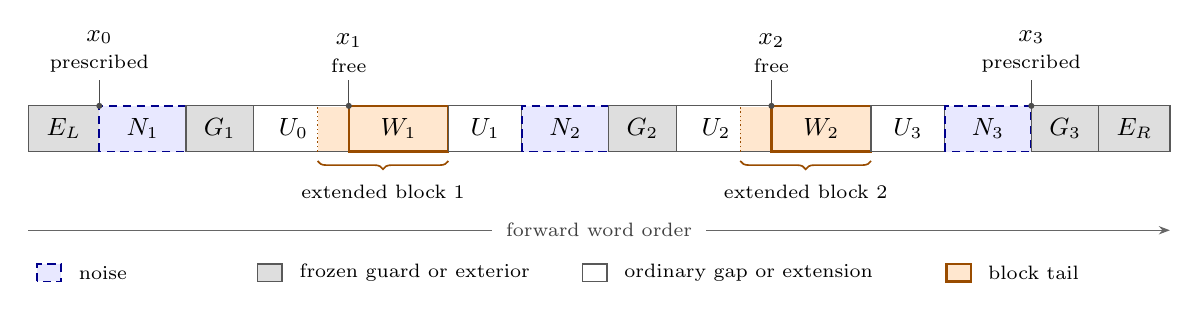
\begin{tikzpicture}[
  x=1.1cm,y=1cm,
  every node/.style={font=\small},
  frozen/.style={draw=black!65,fill=black!13,line width=.45pt},
  noise/.style={draw=blue!55!black,fill=blue!9,line width=.65pt,densely dashed},
  ordinary/.style={draw=black!65,fill=white,line width=.45pt},
  used/.style={draw=orange!60!black,fill=orange!19,line width=.8pt},
  extension/.style={fill=orange!19},
  height/.style={font=\small,align=center,inner sep=1pt},
  package/.style={decorate,decoration={brace,mirror,amplitude=3pt},
                  draw=orange!60!black,line width=.6pt}
]
  \path[frozen] (0,0) rectangle (.82,.58);
  \path[noise] (.82,0) rectangle (1.82,.58);
  \path[frozen] (1.82,0) rectangle (2.60,.58);
  \path[ordinary] (2.60,0) rectangle (3.70,.58);
  \path[extension] (3.34,.01) rectangle (3.70,.57);
  \draw[orange!60!black,densely dotted,line width=.55pt]
    (3.34,0)--(3.34,.58);
  \path[used] (3.70,0) rectangle (4.85,.58);
  \path[ordinary] (4.85,0) rectangle (5.70,.58);
  \path[noise] (5.70,0) rectangle (6.70,.58);
  \path[frozen] (6.70,0) rectangle (7.48,.58);
  \path[ordinary] (7.48,0) rectangle (8.58,.58);
  \path[extension] (8.22,.01) rectangle (8.58,.57);
  \draw[orange!60!black,densely dotted,line width=.55pt]
    (8.22,0)--(8.22,.58);
  \path[used] (8.58,0) rectangle (9.73,.58);
  \path[ordinary] (9.73,0) rectangle (10.58,.58);
  \path[noise] (10.58,0) rectangle (11.58,.58);
  \path[frozen] (11.58,0) rectangle (12.36,.58);
  \path[frozen] (12.36,0) rectangle (13.18,.58);

  \foreach \pos/\lab in {
    .41/E_L,1.32/N_1,2.21/G_1,3.06/U_0,4.275/W_1,5.275/U_1,
    6.20/N_2,7.09/G_2,7.94/U_2,9.155/W_2,10.155/U_3,
    11.08/N_3,11.97/G_3,12.77/E_R}
    \node at (\pos,.29) {$\lab$};

  \foreach \pos/\lab/\kind in {
    .82/x_0/prescribed,3.70/x_1/free,8.58/x_2/free,11.58/x_3/prescribed}{
    \draw[black!70,line width=.45pt] (\pos,.58)--(\pos,.91);
    \fill[black!70] (\pos,.58) circle (1.1pt);
    \node[height,anchor=south] at (\pos,.96)
      {$\lab$\\[-1pt]{\scriptsize \kind}};
  }

  \draw[package] (3.34,-.12)--(4.85,-.12)
    node[midway,below=5pt,font=\scriptsize] {extended block 1};
  \draw[package] (8.22,-.12)--(9.73,-.12)
    node[midway,below=5pt,font=\scriptsize] {extended block 2};

  \draw[-{Stealth[length=4pt]},black!60,line width=.45pt]
    (0,-1.00)--(13.18,-1.00);
  \node[fill=white,inner xsep=5pt,font=\scriptsize,text=black!75]
    at (6.59,-1.00) {forward word order};

  \path[noise] (.10,-1.65) rectangle (.38,-1.43);
  \node[anchor=west,font=\scriptsize] at (.47,-1.54) {noise};
  \path[frozen] (2.65,-1.65) rectangle (2.93,-1.43);
  \node[anchor=west,font=\scriptsize] at (3.02,-1.54)
    {frozen guard or exterior};
  \path[ordinary] (6.40,-1.65) rectangle (6.68,-1.43);
  \node[anchor=west,font=\scriptsize] at (6.77,-1.54)
    {ordinary gap or extension};
  \path[used] (10.60,-1.65) rectangle (10.88,-1.43);
    \node[anchor=west,font=\scriptsize] at (10.97,-1.54) {block tail};
\end{tikzpicture}

\caption{Forward word arrangement for two used blocks in
\eqref{ker:two-block-word}.  The shaded terminal portions of \(U_0\)
and \(U_2\) are the left extensions: each and its adjacent \(W_i\)
form one extended protected block, as indicated by the braces.
Each \(W_i\) includes the block's right extension.
The heights \(x_0,x_3\) are prescribed; \(x_1,x_2\) are free at the
used starts.  Segment widths are schematic.}
\label{ker:word-arrangement-figure}
\end{figure}

The conditional experiment has four groups of variables:
\begin{enumerate}[label=(\roman*)]
\item the frozen exterior \(e\), including guards, search origins and
      discovered noise endpoints;
\item the ordinary raw words and their duration/cut variables \(\theta\),
      with every left extension kept in its protected block;
\item the forest value and the remaining full-height coordinates;
\item the noise words, sampled conditional on the endpoints determined
      by the preceding variables.
\end{enumerate}
The braces in the figure identify constituent time blocks. All blocks
from one spatial buffer, together with their forest data and joint
readouts, belong to the single package in
\eqref{ker:reference-packages}.

For the fixed surrogate typing rule described below, set
\[
 u_1=d(G_1U_0),\quad
 u_2=d(W_1U_1G_2U_2),\quad u_3=d(W_2U_3).
\]
All these are functions of the ordinary raw words \(w\), the guards,
and the fixed instruction, independent of the free heights and
noise paths.  The forward noise displacements are exactly
\begin{equation}\label{ker:triangular-heights}
 \Delta_1=x_1-x_0-u_1,\qquad
 \Delta_2=x_2-x_1-u_2,\qquad
 \Delta_3=x_3-x_2-u_3.
\end{equation}
The first two equations are an affine triangular integer bijection;
the third imposes the terminal displacement.  In particular
\(H_i=\Delta_i^1\), while the second \emph{backward} displacement
is \(-\Delta_i^2\).  The noise lengths \(k_i\) are fixed by their
recorded endpoints.  General finite collections give the same formula
\(\Delta_i=x_i-x_{i-1}-u_i\), with one final equation only when the
terminal height is prescribed.  All even-cut and displacement parities
are retained.  In particular the feasible condition is
\(k_i-\Delta_i^1+\Delta_i^2\in2\Z\).

\paragraph{The augmented reference and its exact weight.}
Use the same point masses for the deterministic absolute cuts of the
instruction. Within each aggregate package, choose positive smooth
reference densities for its free absolute cut coordinates in a
product of the windows just chosen, independently between disjoint
spatial buffers. Compute all durations and relative cuts from these
coordinates; do not independently sample durations linked by a fixed
cut. After the exterior endpoints are frozen, compute genuine gap
remnants from the remaining intervals. The boxes are small enough
to leave these remnants positive on the good neighborhood.
Draw the ordinary raw words with their iid letter weights.  The
additional gap/cut laws give an exact joint mass \(r_n(e,\theta)\).
Alternatively a proposal outside the fitting region may be completed
by a dummy remnant and assigned weight zero; it is not conditioned
on successful placement. Thus the aggregate packages retain their
independent reference marginals across disjoint spatial buffers.
Free cut coordinates remain integrated, and instruction-fixed cuts
retain their point masses. Thus the reference and actual mark laws
have the same deterministic support; the ratio
\(\chi_n(e,\theta)/r_n(e,\theta)\) contains only the free-coordinate
mass ratio after their identical deterministic indicators cancel.

Draw the raw forest value \(v_F=P_Fx\) with its exact normalized
mass \(\beta_n(v_F\mid\theta)\), corresponding to the smooth density
on \(s_bn^{-1/2}\Lambda_F\).  On each full-height fibre draw \(x\)
with a positive smooth lattice mass \(f_n(x\mid v_F,\theta)\).
A concrete choice is a normalized Gaussian in
\(s_b(x-Sv_F)/\sqrt n\), where \(S\) is an integer-linear right
inverse of \(P_F:\Lambda_m\to\Lambda_F\).  Such an \(S\) exists
because its image is a free abelian group.  Its fibres are translates
of the fixed kernel lattice, so this choice has the required smooth
limiting conditional density and constant coarea factor.

Compute \eqref{ker:triangular-heights}.  At feasible endpoints sample
independent noise words with laws
\(\mathsf B_{H_i,k_i,-\Delta_i^2}\).  At any impossible endpoint use
a fixed dummy probability law and give it weight zero.  This avoids
conditioning the protected reference words on endpoint feasibility.
The resulting probability measure is \(R_n^e\).

Initially let \(A_n\) include all actual restrictions: fitting and
cut instructions, the selected tube, admissible depths, true flexible
resolutions, and, in the finite case, empty reduction.  The exact
weight for \eqref{ker:two-block-word} is
\begin{equation}\label{ker:finite-weight}
 W_n^e=
 \frac{\chi_n(e,\theta)}
 {r_n(e,\theta)\,\beta_n(v_F\mid\theta)\,
                         f_n(x\mid v_F,\theta)}
 \prod_{i=1}^{3}\!\left[
   \pi_n(\Delta_i^1)\,
   p_{\Delta_i^1}(k_i,-\Delta_i^2)\right]\1_{A_n}.
\end{equation}
It is zero off actual support.  The same expression has one factor
per noise in the general case.

To verify the identity, multiply \eqref{ker:finite-weight} by an
atom of \(R_n^e\).  The cut, forest, and fibre reference masses cancel.
Each noise endpoint mass cancels the denominator of its conditional
word law, leaving \(\mathfrak p(N_i)\) with its intrinsic ladder
restriction.  The remaining ordinary-word product is already its
iid weight.  Frozen guards contribute the fixed factors
\(\mathfrak p(G_i)\), which cancel upon conditioning.  Their
backward-discovered stopping locations are exactly their intrinsic
\(\mathcal L_H\) restrictions, so no further stop-selection factor
is missing.  What remains is the actual independent cut/depth marking
mass times the raw-word product and \(\1_{A_n}\).
Therefore the actual marked conditional law is exactly
\[
 Q_n^e=\frac{W_n^e}{R_n^e[W_n^e]}R_n^e.
\]
For the finite bridge its original empty-word normalizer also cancels.
No asymptotic assertion is used in this finite calculation.

\paragraph{Removing microscopic admissibility from the weight.}
Internally reduce each guard together with its following ordinary
stretch.  Give every still-unresolved flexible order the type assigned
by a fixed finite rational comparison partition.  This is a
deterministic rule of the ordinary raw letters, their time slots,
and the instruction, fixed before sampling heights or noise words.
The partitions are refined with those for the protected used portions.
In particular the \(u_i\) in \eqref{ker:triangular-heights} are literal
functions of \(w,e,\theta\), not functions of \(x\) or the noise paths.

An order still unresolved after that internal reduction has both
candidate suppliers before the guard's start.  A later available
burger would instead have resolved it internally.  The positive
guard duration gives both candidates a positive backward span.
On a compact supplier window, Lemma~\ref{enc:chord-genericity}
excludes equal supplier endpoints and branch ambiguities; its
compactness argument yields the finite comparison partition with
strict chronological clearance.  Choose the contour tube small
enough to preserve those comparisons.  If a proposed surrogate
configuration passing that tube had a first wrong flexible type,
its preceding contour would be the true contour.  Its two actual
supplier records would then have the prescribed strict chronological
order, forcing the prescribed type, a contradiction.  This induction
applies to every admitted raw configuration, including independently
sampled reference words.  Internal matches agree automatically.
The protected-used type lists obey the same buffered argument, so
their readouts agree with the actual incidence record on the tube.

For the finite bridge, choose positive integer floors \(\ell_1,\ell_2\)
below the prefix counts and below all mutable contour heights.
The bottom \(\ell_c\) prefix burgers of each type, including their
chronological interleaving across types, are then preserved by every
admitted mutable word.  Impose the same exact endpoint counts at the
last noise.  Choose a fixed suffix cut \(t_c<T\) where both original
counts are below their respective floors.  Such a cut exists by
continuity at the excursion endpoint, and the portion up to \(t_c\)
retains positive interior margins.  Internally reduce the final guard
together with the entire following suffix segment up to \(t_c\),
and apply the same fixed comparison partition to its unresolved
flexible orders.  Their candidate suppliers precede the guard's
start, so its positive duration and the first-error argument give
the correct suffix types up to this cut.

Here is the exact remaining inventory invariant.  Two mutable words
may leave different burgers above the protected floors, but have the
same counts.  Along the common typed suffix their counts stay equal.
When a type's count first reaches its floor, all potentially different
survivors above that floor have been removed by the last-in-first-out
rule.  Subsequent survivors of that type are common protected-prefix
burgers and identically created suffix burgers.  At \(t_c\) this has
happened for both types.  Their identities and creation order agree,
so the entire chronological inventories agree.  The rest of the raw
suffix consequently evolves identically, including absent-candidate
cases, and has the original empty reduction.  Equality of high-rank
burger identities before \(t_c\) is not asserted or needed.

Thus, on this good chart, the true-resolution and empty-reduction
parts of \(A_n\) are automatic.  Its remaining conditions are the
specified cut, depth, positivity, fitting, and uniform-tube tests,
chosen with continuum continuity boundaries.  There is no residual
microscopic freshness or success-normalization factor.

\paragraph{The reference limit and its explicit weight.}
Start with the aggregate package limits
\eqref{ker:reference-packages}. Their input \(\mathsf I\) contains the
relative contour of every complete extended block, including the
portions called left extensions in the display. Its cut coordinates
are within-block offsets. Keep each block's remaining absolute
placement, all omitted-gap durations, the scaled full heights
\(x/\sqrt n\), the genuine gap paths and the noise paths in an
auxiliary variable \(A\). Whole-contour tests will be read from the
assembled paths and are retained in \(A\) as well.

Conditional on its duration and internal cut offsets, each iid raw
block and its time-labelled readout are invariant under a common
translation of that block's time indices. The aggregate readout uses
only these relative block data, the forest parameter and the fixed
instruction. Thus the remaining placements reveal no additional
output information. Disintegrate the absolute-cut reference law into
the retained relative cut data and those placements. On an interior
good cell this is an affine change of the free cut coordinates, with
the deterministic atoms retained. Its smooth lattice densities and
fixed affine fibres give a limiting conditional placement law through
the input alone; no continuity of the output kernel is required.

For a fresh ordinary word, two choices of its externally unresolved
flexible types change its contour by at most the number of flexible
orders unidentified by internal reduction. The reduced-word maximal
and unidentified-order estimates
\cite[Lemma~3.13]{SheffieldInventory}
\cite[Lemma~3.7]{GwynneMaoSunFKI} make this error
\(o_{\PP}(\sqrt n)\), uniformly on the finitely many fresh pieces.
The bound does not depend on the external inventory or on its chosen
types. A ladder guard is intrinsically resolved. On the good tube the
frozen typed pieces agree exactly with their actual contours by the
first-error and protected-floor arguments above. Their rescaled paths
are part of the frozen macroscopic record \(e\).
Consequently each \(u_i/\sqrt n\) in
\eqref{ker:triangular-heights} is, up to \(o_{\PP}(1)\), a sum of
increments from \(\mathsf I\), fresh gap paths, and \(e\).
There is no residual dependence on a microscopic exterior inventory.

Fresh gap paths are appended through Brownian increment laws.
The fibre Gaussian is an input-dependent kernel with a smooth limit.
Conditional noise paths have the compact-uniform bridge limits of
\Cref{ker:ladder}, at endpoints determined by the preceding inputs.
A backward bridge \(B\) of duration \(k\) gives forward contour
\(B(k-t)-B(k)\), a continuous path transformation. Thus, on each
interior compact parameter set, these additions converge through a
kernel \(T_e(\mathsf I,\dd A)\). The complete reference limit has form
\begin{equation}\label{ker:augmented-reference-limit}
 \left[\prod_\alpha\mathcal R_\alpha(\dd\mathsf I_\alpha)\right]
 T_e(\mathsf I,\dd A)
 \prod_\alpha K^0_\alpha(\mathsf I_\alpha,\dd O^0_\alpha).
\end{equation}
This is the reference factorization required in
\Cref{ker:density-ratio}. The same construction retains each bounded
continuous test of the assembled whole contour. It does not assert
independence between the time blocks within a union buffer.

On interior compact parameter sets, \(H_i/\sqrt n=a_i>0\),
\(k_i/n=t_i>0\), and \(-\Delta_i^2/\sqrt n=y_i\) give
\[
 p_{H_i}(k_i,-\Delta_i^2)
 =2n^{-3/2}a_i^{-3}g(t_i/a_i^2,y_i/a_i)+o(n^{-3/2})
\]
uniformly on the feasible parity coset.  The depth masses are
\(n^{-1/2}\) times their positive limiting density. The reference
cut, forest, and fibre masses have their exact lattice normalizers.
The identical deterministic-cut masses in the actual and reference
laws have already canceled. Conditional on the fixed cut counts,
the actual joint Poisson mark density and the positive reference
density on the free-coordinate boxes have a bounded smooth ratio
on interior compact sets; the actual mark density need not factor
between packages. After their common powers of \(n\) are removed,
these free-coordinate masses and the forest and fibre masses
converge to their positive smooth densities. Fixed durations
contribute no duration-density factor; the ladder estimate above is
uniform also when such a duration is held at a prescribed positive
value. The factors in
\eqref{ker:forest-units}--\eqref{ker:hitting-units} record every fixed
height Jacobian.  Thus \eqref{ker:finite-weight}, after canceling a
common exterior-only factor, is bounded and converges jointly to a
weight depending only on macroscopic inputs.  The translations
\(u_i/\sqrt n\) have that same property by the surrogate contour
estimate for fresh pieces and the retained macro paths for frozen
ones.  Lemma~\ref{ker:ladder} gives compact-uniform convergence of
the conditional noise paths. The aggregate fresh-package laws are
independent of the microscopic exterior, the frozen rescaled paths enter only through \(e\), and the
noise limits are uniform on these compact parameter sets. Hence the
factorization and weight convergence hold along every convergent
sequence of good microscopic exteriors, not only at each fixed
exterior value.

If an unused full height is integrated out, its denominator
\(f_n(x\mid v_F,\theta)\) in \eqref{ker:finite-weight} must first be
included.  Fibre summation in the weighted joint measure then cancels
that sampling density; its lattice Riemann sum has constant coarea.
Whole-contour tests and their conditional bridge factors remain
inside this integration.  Equivalently keep the scaled height in
\(A\) through Lemma~\ref{ker:density-ratio} and integrate it afterward.
The protected output depends on full heights only through \(v_F\),
so neither procedure introduces an output-dependent fibre factor.
Random cut coordinates likewise remain integrated input variables
throughout, while deterministic cuts remain fixed parameters.

The limiting normalizer is positive. Realized depths and durations
are positive, and the strict tube contains a product subtest open
in the free cut coordinates and in the free Brownian pieces and
first-passage bridges. Deterministic cuts are held fixed in this
subtest; if there are no free cuts, their factor is a point mass.
The positive free-coordinate and endpoint densities and path support
give positive weight, stably for nearby exterior records.
Lemma~\ref{ker:density-ratio} now applies.
Finally exhaust under the actual contour law with its once-drawn
independent marks: almost every realization has a finite protected
cover, positive gaps, the proved local instructions, and noises fitting
for sufficiently small raw depth \(a\).  Finite collections of good
chart neighborhoods and interior compact cutoffs cover probability
at least \(1-\varepsilon\).  Their omitted contribution to a bounded
conditional-identity test is at most its bound times
\(\varepsilon\); let \(\varepsilon\downarrow0\).
All whole-contour observations are retained in \(A\), completing the
proof.
\end{proof}


\subsection{Proof of the local-kernel theorem}

\begin{proof}[Proof of \Cref{ker:local-kernels}]
Use the aggregate kernels \(K^0\) constructed in
\eqref{ker:reference-packages}. By \Cref{ker:word-ratio}, their
augmented reference law has form
\eqref{ker:augmented-reference-limit}, and its limiting change of
density depends only on the retained inputs. Applying
\Cref{ker:density-ratio} therefore preserves these kernels under the
actual word law. The recovery \(\mathsf I=\mathsf I(I)\) and the
spatial relabelling described above give \(K(I,\dd O)\).
Multiplying a reference law by a positive smooth function of its input
and normalizing leaves its conditional output law unchanged.  Thus
changing the auxiliary densities, and integrating parameters unused
by the readout, identifies the kernels on overlapping input laws.

For a finite family of disjoint buffers, the aggregate reference
packages, including their full inputs and output arrays, are independent.
Their joint limits are products.  Apply Lemma~\ref{ker:word-ratio}
to their union: the limiting resampling density depends only on the
continuum input, so Lemma~\ref{ker:density-ratio} preserves that
conditional product.  The same calculation applies in the finite
bridge.  Tests of the whole contour can be kept in the calculation;
a monotone class of bounded continuous tests and the determination
in Theorem~\ref{enc:peanosphere} identify conditioning on
\(\mathcal C\).  No additional information in \(\mathcal C\) changes
the kernel.  Finite-dimensional products determine the assertion for
countable arrays.

Compatibility is obtained before limiting.  When two charts describe
the same finite test, their readouts are restrictions of the same
union incidence record and coincide on its good event for all large
indices.  The good-event exhaustion in Lemma~\ref{ker:word-ratio}
transfers this equality to the limits.  Countably many such equalities
hold simultaneously, and remain so under an absolutely continuous
change of input law.  This constructs one compatible array, not a
collection of unrelated conditional versions.

For bounded changes of field density, multiply joint continuous tests
by the density, first approximating that density in probability by
bounded continuous functions of the input.  Truncate an integrable
density to remove boundedness.  This proves the third assertion.
Local marks can be retained first and then integrated with their
conditional laws.  Independent marks in disjoint regions preserve
the conditional product.

For fixed offsets include their scaled versions in the same aggregate
reference experiment before extraction. Its finite joint laws retain
the actual correlations between these offsets; independence is used
only between disjoint spatial buffers.

A measurable continuum functional has its fixed joint law with the
input. On a set of input probability at least \(1-\varepsilon\),
Lusin approximation replaces any bounded test of that functional by
a continuous one. Include these approximations in the extraction and
let \(\varepsilon\) tend to zero. Finally, variables sampled
conditionally on \(\mathcal C\), independently of the discrete outputs,
can be appended by disintegration. This proves the final assertion.
\end{proof}

\subsection{Order and ordinary-field transfer}

\begin{lemma}[Finite traversal order]\label{ker:finite-order}
For a compact protection \(K\) in a bounded open real buffer \(V\),
only finitely many traversals of \(V\) meet \(K\), almost surely.
After retaining their local directed pieces, their remaining global
order is a finite permutation.  Conditional on the local imaginary
input \(J\), write
\[
 w_o(J)=\PP[\text{order}=o\mid J].
\]
Its feasible values are those with \(w_o(J)>0\); the actual order is
feasible almost surely.  These weights depend neither on the real
field nor on the choice of quantum time unit.

For every finite protected test, the necessary order is determined
by the imaginary field in a sufficiently large finite buffer, on
events whose probabilities tend to one as that buffer increases.
The number of traversals can also be bounded deterministically on
an exhaustion of probability tending to one.

The kernels can be augmented to include an output for every feasible
order, simultaneously for all retained fixed scale offsets.  Given
the entire real and imaginary fields, the law of this augmented
vector depends only on their respective local restrictions; such
vectors have product laws in disjoint buffered regions.  One component
is the actual output at the actual order.
\end{lemma}

\begin{proof}
Properness places all visits to \(K\) in a compact time interval.
Uniform continuity there supplies \(\delta>0\) such that moving
between \(K\) and \(V^c\) takes at least \(\delta\) units of time.
Each distinct traversal meeting \(K\) contains such a move, so only
finitely many occur.  Lemma~\ref{enc:local-exploration}
reads their directed pieces in any strict imaginary enlargement.
They can be enumerated measurably by taking the first representative
in the fixed dense-point enumeration defining the local flow-line
construction.  The global curve order is determined by the imaginary
field before it is parameterized by quantum area.  Hence its
conditional probabilities given \(J\) have the stated independence
of real-field and clock choices.  For a finite conditional distribution,
\(\PP[w_O(J)=0]=0\), which proves feasibility.

For completeness, order determination can be witnessed in a finite
region.  For the finitely many representatives, trace their left and
right frontier flow lines until the corresponding same-angle branches
have merged.  The whole-plane flow-line tree construction of
space-filling SLE gives these mergers at finite times almost surely;
the resulting finite trees and their cyclic sides determine the
relative Peano order \cite{MillerSheffieldIGIV}.  Their compact traces lie in a
finite disk.  Until exit from a slightly larger disk they are local
sets determined by the imaginary field there, so the witnessed order
is determined there as well.  For increasing deterministic disks,
the probability that all of these finitely many witnesses are
contained tends to one.  Intersecting with deterministic bounds on
the number of representatives proves the exhaustion assertion.

By Theorem~\ref{ker:local-kernels}, conditional on the whole fields
and order \(o\), the actual local output array has a kernel
\(K_o(I,\dd O)\), where \(I\) now omits the order.  This is defined
for almost every local input with \(w_o(J)>0\).  Keep the actual
component and, conditionally on the fields and that component,
sample each of the other feasible components independently from its
kernel.  The entire vector then has conditional law
\(\prod_{o:w_o>0}K_o(I,\dd O_o)\), which is independent of the actual
order and depends only on local restrictions.  The same construction
uses the joint array at all retained fixed scale offsets, so it does not
alter their within-order consistency.  Conditional products between
disjoint regions follow from Theorem~\ref{ker:local-kernels}, using
independent auxiliary fills.  This proves the last assertion.
\end{proof}

\begin{lemma}[A single traversal near a simple visit]\label{ker:single-traversal}
Suppose \(z\) has a unique exploration preimage.  For every bounded
neighborhood \(V\) of \(z\), all visits to some smaller neighborhood
\(U\) of \(z\) lie in one traversal of \(V\).  Protected observations
therefore require no permutation input near \(z\); their kernels
are measurable from the real and imaginary restrictions in every
fixed sufficiently small surrounding buffer.
\end{lemma}

\begin{proof}
Let \(t\) be the unique preimage, and let \((a,b)\) be the component
of \(\eta^{-1}(V)\) containing \(t\).  If every neighborhood of \(z\)
had a visit outside \((a,b)\), properness would give a convergent
sequence of such times.  Its limit would be a preimage of \(z\)
outside \((a,b)\), contradicting uniqueness.  Thus all visits to
some \(U\) lie in that component.  Within a single directed traversal,
order is its own direction; labelled length differences are intrinsic
to its local frontiers.  The local measurability assertion follows
from Lemma~\ref{enc:local-exploration} and
Theorem~\ref{ker:local-kernels}.
\end{proof}

\begin{proposition}[Field and unit changes]\label{ker:field-transfer}
On strict buffered compact subsets away from marked singularities,
ordinary GFF restrictions, cone restrictions in an appropriate fixed
chart, and their finite smooth shifts are locally mutually absolutely
continuous.  Restrictions on finitely many separated buffers are
jointly equivalent to independent ordinary restrictions.  The same
statements hold for the independent imaginary field modulo its
angular period, using its uniform phase.  These changes transfer the
kernels of Theorem~\ref{ker:local-kernels}, their products, and the
all-order vectors of Lemma~\ref{ker:finite-order}.

The kernels are intrinsically covariant under affine coordinate
changes.  For \(\psi(z)=az+b\), \(a\ne0\), transform simultaneously
\[
 h\longmapsto h\circ\psi+Q\log|a|,\qquad
 \widetilde h\longmapsto\widetilde h\circ\psi-\chi\arg a,
 \quad \chi=2/\gamma-\gamma/2.
\]
Transform ports and ranges by \(\psi^{-1}\).  Quantum durations,
frontier lengths, raw graph costs, and flag-surface extremal lengths
are unchanged.  In particular translations preserve every chosen
deterministic cost unit.

There is also an exact indexed change of quantum units.  If the
original time unit is \(n\) and the cost denominator is \(c_n\),
express the same map using time unit \(vn\) and cost denominator
\(c_nv^p\).  Its field input, time labels, frontier lengths, and costs
become, respectively,
\begin{equation}\label{ker:units}
 h_v=h-\gamma^{-1}\log v,\qquad
 t_v=v^{-1}t,\qquad \ell_v=v^{-1/2}\ell,
 \qquad O_v=v^{-p}O.
\end{equation}
These identities hold jointly for the indexed kernel arrays.  They
also hold with \(h+b\) in place of \(h\).  They assert a re-expression
of the same array, not equality of two differently indexed kernels.
For any other deterministic output denominator \(d_{n,v}>0\), the
last factor is instead its literal ratio \(c_n/d_{n,v}\); in
particular extremal length divided by the same denominator in both
conventions has no additional power of \(v\).
\end{proposition}

\begin{proof}
Take larger disjoint disks around the compact buffers, with a pin
outside them.  Conditional on the exterior GFF, the fields in the
disks are independent zero-boundary GFFs plus harmonic functions.
Each harmonic function on a strict inner buffer has a smooth
finite-energy extension supported in its disk.  Conditional
Cameron--Martin equivalence and then integration show that the joint
restrictions are equivalent to independent zero-boundary restrictions.
For the cone comparison, choose the normalization tests strictly
inside its normalization circle and their buffers away from its
marked center.  There the field is an ordinary GFF plus the
logarithmic drift, which has a finite-energy cutoff on the buffers.
The same argument applies there and to its coordinate images.  Finite smooth shifts are directly Cameron--Martin changes.
For the imaginary field use its Markov decomposition modulo the
angular period, with an independent uniform phase
\cite[Propositions~2.8, 2.9 and~2.11]{MillerSheffieldIGIV}.  The argument applies to
its harmonic part too.  Densities can be truncated and integrated as
in Theorem~\ref{ker:local-kernels}.

For affine covariance, express one intrinsic chart in its two
coordinates.  The quantum coordinate rules identify its area and
labelled boundary lengths, and imaginary geometry identifies its
directed frontiers.  The retained raw incidence record and triangle
shapes are literally the same; only their spatial labels change.
Consequently their finite observations agree before extraction.
Taking joint limits proves covariance of the kernels.  The uniform
phase convention makes translations and positive dilations exact
symmetries of the unclocked whole-plane imaginary input.  Absolute
continuity alone would not prove this covariance; here it follows
from the intrinsic finite readouts.

Finally, dividing quantum area units by \(v\) subtracts
\(\gamma^{-1}\log v\) from the field and divides boundary-length
units by \(\sqrt v\).  Changing the denominator by \(v^p\) gives the
last identity in \eqref{ker:units} exactly on the same finite map.
For integer time units use \(v_n=\lfloor vn\rfloor/n\) throughout
this identity and retain the same raw cuts.  Then \(v_n\to v\).
If Poisson cuts are used, transform their intensity by the same
clock change; include all required intensities in the countable
atlas before extraction.  Thus there is no endpoint-rounding error
measured in an arbitrary graph-cost unit.  Passing to the joint
indexed limit proves the formula.  No relation between \(c_n\) and
\(c_{\lfloor vn\rfloor}\), or scaling rule for an unindexed passage
limit under addition to \(h\), is used.
\end{proof}

\subsection{A diagonal with varying volume labels}

\begin{proposition}[Fixed normalized inputs in a varying-label diagonal]
\label{ker:normalized-diagonal}
Let \(v_r>0\) be deterministic volume labels. For each \(r\), take an
unconditioned joint law supplied by \Cref{ker:local-kernels},
re-expressed in the units of \eqref{ker:units}. Suppose its base field
in those units has one fixed ordinary normalized reference law,
including the same imaginary-field law with uniform phase. Draw the
observation marks using the same normalized convention at every row.
A joint diagonal may retain every
fixed relative offset in a countable list, provided every retained
effective microscopic time unit tends to infinity.
The output denominators may be arbitrary deterministic positive
numbers. The resulting limits have the compatible kernels and the
conditional product property of \Cref{ker:local-kernels}, and may
retain fixed measurable continuum functionals and the all-order
arrays of \Cref{ker:finite-order}.
\end{proposition}

\begin{proof}
Fix the ordinary normalized reference input
\(h_*\) and its imaginary input with uniform phase. Choose common
smooth auxiliary forest and free-cut laws for the reference
experiments, keeping each instruction's deterministic cuts fixed.
The density invariance in \Cref{ker:local-kernels}(3)
allows this choice without changing the resulting actual-law kernels
or prescribed observations. The observation marks themselves use the
fixed normalized convention in the statement. Independent reference restrictions
are used in the disjoint enlarged buffers.  At label \(v_r\), sample
\(h_*\) in that label's unit convention.  In the original convention
this is \(h=h_*+\gamma^{-1}\log v_r\); the indexed unit identity
\eqref{ker:units} then gives \(h_{v_r}=h_*\).  Thus the label changes
the effective microscopic time and cost units, while the base
normalized input has a fixed law.
Write \(P_r\) for these unconditioned row laws and \(\nu\) for
their common marginal of continuum inputs and once-drawn marks.
Thus \(\pi_{\rm input}P_r=\nu\) for every \(r\).

At stage \(r\) retain the first \(r\) coordinates and relative
offsets \(w_1,\ldots,w_r\).  First hold \(r,v_r\) fixed.  The
fixed-label construction supplies microscopic approximants for that
row's unconditioned joint law, including its protected reference
experiment and reference metric observations.  Choose an approximant
along the sequence defining that row, with base integer scale
\(n_r\), so that the first \(r\) bounded joint
tests have error at most \(2^{-r}\) and
\[
 N_r=n_rv_r\longrightarrow\infty,\qquad
 n_rv_r\min_{j\le r}w_j\ge r.
\]
Include the corresponding protected-density tests among those
approximated.  For integer-time conventions keep each raw cut and readout exactly and
round only the unit used to scale its labels.  Since the smallest
unit tends to infinity, this changes the continuum labels by
\(o(1)\); it changes no edge or path cost.

Re-expressed in the effective unit \(N_r\), these approximants form
one raw-word sequence with a fixed continuum reference input law and
arbitrary deterministic output denominators \(c_{n_r}v_r^p\).
For any fixed finite list of offsets, its joint field inputs are
\(h_*-\gamma^{-1}\log w_j\), a law independent of \(r\).
Apply Lemma~\ref{ker:word-ratio} directly to this sequence.
Its durations, forest variables, guards, noise depths, and ladder
limits are all expressed in \(N_r\) units; in particular its raw
depth window is proportional to \(\sqrt{N_r}\).  Its reference densities are
fixed, and its compact good-chart normalizers have the positive
limits proved there.  The diagonal macro-input marginals converge
to \(\nu\).  Its actual-law good-chart exhaustion is therefore
uniform along this sequence: first fix finitely many
\(\nu\)-continuity good cells of total mass at least
\(1-\varepsilon\), then let \(r\) tend to infinity, and
finally let \(\varepsilon\) decrease to zero.  A finite union handles
any fixed finite list of buffers and offsets.  The exact resampling
identity and independent complete reference packages therefore prove
the conditional product for this diagonal directly.  Summable joint
test approximation identifies the result with the desired limit of
the unconditioned row laws.  Subsequent fixed locally absolutely
continuous field changes use \Cref{ker:local-kernels}(3).  No assertion is
made here for arbitrary varying field densities.

The fixed measurable functionals are retained by the Lusin argument
in \Cref{ker:local-kernels}, now under the common input marginal
\(\nu\). The finite-order augmentation uses that same fixed imaginary
marginal and the joint retained array. Thus it also applies to the
diagonal, without changing any actual-order coordinate.
\end{proof}

\subsection{Normalized sphere heights and selected changes}

\begin{lemma}[Actual-height sphere densities]\label{ker:sphere-density}
Use the sphere chart with the exploration root at infinity and two
further area marks at \(0,1\).  On a finite union \(K\) of separated
closed disk patches avoiding the marks, the restriction of the
normalized sphere field is dominated by the corresponding ordinary
real-field restriction.  Its density is strictly positive precisely
on the ordinary restrictions for which
\(\mu_h(K)<1\).  Boundaries may be chosen to have zero mass.
The joint law, including imaginary restrictions on separated strict
buffers, is therefore equivalent on this mass event to independent
ordinary real and imaginary restrictions on the patches.

Together with their common conditional kernels, the same domination
and positivity hold for any finite or countable protected output
arrays in the actual finite-sphere subsequential law.  Every patch
keeps its actual additive height and its original deterministic cost
and time units.
\end{lemma}

\begin{proof}
By Proposition~\ref{enc:sphere-representation}, before normalization
write the field as \(h_0+d\), where \(h_0\) is an ordinary whole-plane
GFF with a pin, \(d\) is the deterministic marked drift, and the law
has a strictly positive integrable tilt.  Normalization gives
\[
 h=h_0+d-\gamma^{-1}\log\mu_{h_0+d}(\Chat).
\]
Repin outside \(K\) first.  The change is an additive random constant,
which cancels in this normalization; its effect on the original tilt
is another positive integrable density.  We may therefore use an
exterior pin throughout the following Gaussian calculation.

Choose a smooth finite-energy \(g\) with \(0\le g\le1\), equal to
one precisely on \(K\), less than one off \(K\), and zero on an
open set near the pin.  It can be compactly supported away from the
marks.  Orthogonal Gaussian decomposition in the direction \(g\)
gives \(h_0=h_\perp+Xg\), with \(X\) a nondegenerate Gaussian
independent of \(h_\perp\).  Conditional on \(h_\perp\), set
\(\nu=\mu_{h_\perp+d}\).  This is a finite measure of full support,
and its boundary mass on the chosen circles is zero.  On \(K\) the
normalized field is \(h_\perp+d+c(X)\), where
\[
 c(x)=x-\gamma^{-1}\log\int e^{\gamma xg}\,\dd\nu.
\]
Differentiation under the integral gives
\[
 c'(x)=1-
 \frac{\int g e^{\gamma xg}\,\dd\nu}
      {\int e^{\gamma xg}\,\dd\nu}>0.
\]
The inequality is strict because the exterior set where \(g<1\)
has positive mass.  Since \(\nu(\{g=0\})>0\), \(c(x)\to-\infty\)
as \(x\to-\infty\).  Also
\[
 \int e^{\gamma x(g-1)}\,\dd\nu\longrightarrow\nu(K)
 \quad(x\to\infty),
\]
by dominated convergence, so
\(c(x)\to-\gamma^{-1}\log\nu(K)\).
Thus \(c\) is a continuously differentiable increasing bijection
onto that interval, with strictly positive derivative.

Compare the joint variables \((h_\perp,c(X))\) with
\((h_\perp,X)\).  Conditional change of variable gives a density
which is finite and strictly positive exactly when
\(e^{\gamma y}\nu(K)<1\).  This event is the measurable condition
\(\mu_{h_\perp+d+y}(K)<1\) on the resulting patch field.  Pushing
forward therefore proves equivalence of the normalized patch law
with the unnormalized \((h_0+d)|_K\) law restricted to that event.
The initial positive tilt preserves its null sets and positivity.
A finite-energy cutoff of \(d\) away from the marks, and Proposition
\ref{ker:field-transfer}, replace the unnormalized restrictions by
ordinary ones, jointly on all patches.  This proves the real-field
statement at actual heights.

The unclocked imaginary field is independent of the sphere real
field in this chart, by Proposition~\ref{enc:sphere-representation}.
Its separated restrictions are equivalent to independent ordinary
restrictions by Proposition~\ref{ker:field-transfer}; enlarged
imaginary buffers may be chosen before this comparison.  Finally,
Theorem~\ref{ker:local-kernels} attaches precisely the same conditional
output kernels on both sides.  Multiplying a joint input law by a
strictly positive density multiplies the input--output law by that
same density.  This proves the final assertion for the actual sphere
array, including its products and all-vertex escape readouts.
\end{proof}

\begin{lemma}[Dominated transfer after finite selection]
\label{ker:selected-transfer}
Let the real input have one fixed ordinary pinned Gaussian law, and
let \(f_j\) be a finite list of deterministic smooth functions in its
Cameron--Martin space. In particular, for a whole-plane field whose
circle-average pin is fixed outside a bounded region, any smooth
recipe supported in that region is admissible. The pin and its law
are chosen before the auxiliary draws or any event selection.
For recipe \(j\), suppose \(f_j=b_j\) on a preservation buffer
\(V_j\) and \(f_j=0\) outside a larger support buffer \(W_j\).
Before selecting a recipe, sample an auxiliary local output from the
kernel with input \(h+b_j\) in \(V_j\), independently of the original
outputs outside \(W_j\), conditional on the fields.  Use the same
indexed cost and clock array, re-expressed by \eqref{ker:units} when
necessary.

For each recipe, the retained auxiliary interior and original exterior
can be completed to an output with the common conditional law for
\(h'=h+f_j\).  Write
\[
 L_j(h')=\frac{\dd\Law(h+f_j)}{\dd\Law(h)}(h').
\]
After restricting the source to \(L_j(h+f_j)\le L\), the image of
\emph{any} further source event, including a hit event and a rule
selecting recipe \(j\), is a submeasure bounded by \(L\) times the
common output law.  Summing over the finite list gives the bound
\((\#j)L\).  No independence after selection is required.
\end{lemma}

\begin{proof}
Condition on the whole fields.  On \(V_j\), the auxiliary output
has exactly the kernel required by \(h'=h+f_j\); outside \(W_j\),
the original exterior has exactly the unchanged kernel.  Their
product is the corresponding marginal of the common output array,
by Theorem~\ref{ker:local-kernels}.  Countable exterior restrictions
are obtained by exhausting strict buffers outside \(W_j\).
Disintegrate the full common array given these retained restrictions
and sample the remaining coordinates from that conditional law.
This preserves the auxiliary interior and old exterior exactly.
Local Poisson marks may be resampled with the correct conditional
area law in the changed region and retained outside.  The order is
unchanged, since the imaginary field is unchanged.

Before restriction or selection, the resulting pair has law
\[
 \Law(h',O')=L_j(h')\PP_{\rm out}(\dd h',\dd O').
\]
The Cameron--Martin formula for this fixed pinned law gives
\[
 L_j(h')=\exp\{(h',f_j)_\nabla-\tfrac12\|f_j\|_\nabla^2\},
 \qquad
 L_j(h+f_j)=\exp\{(h,f_j)_\nabla+\tfrac12\|f_j\|_\nabla^2\}.
\]
Here the pairing is the Gaussian linear functional. The second formula
expresses the likelihood cutoff directly in the source field. Clipping
this likelihood to \(L\) bounds the entire image measure by
\(L\PP_{\rm out}\).  Restricting the source to any further event
can only decrease its image measure.  This remains true when that
event depends on the original interior, auxiliary draws for other
recipes, a minimizing path, or a selected hit.  The discarded source
coordinates are not required to be independent of the retained ones.
Summing these measure inequalities proves the finite-list bound.
For compactly supported smooth \(f_j\), the Gaussian pairing is
measurable in its support buffer and has variance
\(\|f_j\|_\nabla^2\).  The clipping events can consequently be
included among the fixed continuum tests before selection.
\end{proof}

\section{Simultaneous annuli at prescribed volume scales}
\label{ann:section}

A local estimate with probability close to one must work along every
macroscopic route.  Its volume label and its Euclidean radius are
different parameters.  This section matches them using circle averages
and obtains a linear number of successful, distinct radii around every
point.  All selections of labels are made before revealing the fresh
fields in the selected shells.

Write \(A(a,b)=\{z:a<|z|<b\}\), and fix three shells
\begin{equation}
 E=\overline{A(1/8,4)},\qquad E^+=A(1/16,8),\qquad
 U=A(1/32,16).
 \label{ann:shells}
\end{equation}
The readouts below depend on field restrictions and local kernels in
\(E\); \(U\) is the fresh-field buffer.  Any fixed finite collection of
strictly buffered shell geometries can be placed inside shells with
these roles by changing their fixed radii.  Constants are then allowed
to depend on that collection.

The reference law consists of a zero-boundary real GFF on \(B(0,64)\)
and an independent whole-plane imaginary GFF modulo its angular
period, restricted to \(E\), with the local kernels of
Theorem~\ref{ker:local-kernels}.  The logarithmic covariance
normalization is
\(\Cov(h(z),h(w))=\log|z-w|^{-1}+\text{smooth}\).
The Dirichlet inner product is
\((f,g)_\nabla=(2\pi)^{-1}\int\nabla f\cdot\nabla g\,\dd z\).
An imaginary representative has a circle-average phase in a fixed
interval of length equal to the period.  Subtracting this circle
average leaves the usual centered Gaussian differences.

\subsection{Uniform comparison on a strict interior}

\begin{lemma}[Conditional transfer]\label{ann:conditional-transfer}
Let \(h^0,\widetilde h^0\) be independent zero-boundary GFFs on \(U\).
Add functions \(g,\widetilde g\) harmonic on \(E^+\), with
\[
 \|g\|_{L^2(E^+)}+\|\widetilde g\|_{L^2(E^+)}\le H,
\]
and bounded real and imaginary constants.  On \(E\), retain any fixed
family of the same local output kernels under both field laws.
There is a function \(\omega_H:[0,1]\to[0,1]\), with
\(\omega_H(\varepsilon)\to0\) as \(\varepsilon\downarrow0\), such that
every event of reference probability at most \(\varepsilon\) has
probability at most \(\omega_H(\varepsilon)\) under this shifted fresh
law.  Conversely, for each \(\eta>0\) there is \(p(H,\eta)>0\)
such that every event of reference probability at least \(\eta\) has
shifted fresh probability at least \(p(H,\eta)\).
The constants are uniform in the volume label and in the measurable
event.  They depend on a bound for the two added constants.
\end{lemma}

\begin{proof}
Choose a smooth cutoff supported in \(E^+\) and equal to one near
\(E\).  For a harmonic function \(g\), its product with this cutoff
is an extension in \(H^1_0(U)\), equal to \(g\) on \(E\), whose
Dirichlet norm is at most \(C\|g\|_{L^2(E^+)}\).
Indeed, multiply \(\Delta g=0\) by \(\chi^2g\), integrate by parts,
and use \(2ab\le a^2/2+2b^2\) to bound
\(\int\chi^2|\nabla g|^2\) by
\(4\int g^2|\nabla\chi|^2\); use nested cutoffs for the product
extension.  Constants have extensions of bounded norm by the same
cutoff.  Apply this to both fields in the product Dirichlet space.

If \(P_f\) is the fresh law shifted by such an extension \(f\),
and \(P_0\) the unshifted fresh law, Cameron--Martin and
Cauchy--Schwarz give, for every event \(A\),
\begin{equation}
 P_f(A)\le e^{\|f\|_\nabla^2/2}P_0(A)^{1/2},
 \qquad
 P_f(A)\ge e^{-\|f\|_\nabla^2}P_0(A)^2.
 \label{ann:cm-two-directions}
\end{equation}
These inequalities still hold after adjoining the same conditional
kernel: the likelihood ratio is a function of the fields alone.

Decompose the reference pair on \(U\) by the domain Markov property.
Its harmonic parts, after separating the bounded imaginary phase,
have almost surely finite \(L^2(E^+)\) norms.  Their extensions are
independent of the two fresh parts.  Choose a bound \(H_0\) whose
extension event has probability at least \(1/2\).  Integrating the
second inequality in \eqref{ann:cm-two-directions} gives
\[
 P_{\rm ref}(A)\ge\tfrac12e^{-H_0^2}P_0(A)^2.
\]
The first inequality then bounds the target probability by a constant
times \(P_{\rm ref}(A)^{1/4}\).

For the other direction, if \(P_{\rm ref}(A)\ge\eta\), choose
\(H_\eta\) so that the reference extension exceeds \(H_\eta\)
with probability at most \(\eta/2\).  Integrating the first
inequality gives
\[
 P_0(A)\ge e^{-H_\eta^2}(\eta/2)^2.
\]
The second inequality gives the asserted positive lower bound,
for example \(e^{-H_t^2-2H_\eta^2}(\eta/2)^4\), where \(H_t\)
bounds the target extension norm.  All bounds concern the field
laws and therefore are independent of the output label.
\end{proof}

There is one finite-order issue in applying this lemma.  The
unclocked imaginary input may allow several local traversal orders,
whereas a marginal test uses the actual order.

\begin{lemma}[All feasible orders]\label{ann:all-orders}
For the local arrays of Lemma~\ref{ker:finite-order}, events with
actual-order failure probability at most \(\varepsilon\), uniformly
in their labels, admit augmented all-order events with failure
probability at most \(\omega(\varepsilon)\), where
\(\omega(\varepsilon)\to0\).  Success of the augmented event implies
success for the actual order.  Conditional on both whole fields,
the augmented arrays in disjoint buffered regions have product laws.
\end{lemma}

\begin{proof}
Let \(J\) be the local unclocked imaginary input.  For each feasible
order \(o\) let \(w_o(J)>0\) be its conditional probability and
\(K_o\) its local output kernel.  Lemma~\ref{ker:finite-order}
identifies these weights and kernels: the weights and finite feasible
set depend on \(J\), independently of the real field and volume
label.  Adjoin the other order coordinates as in that lemma, retaining
the actual coordinate, so that the conditional vector law is
\(\prod_oK_o\).

For any \(\zeta>0\), choose \(J_0<\infty\) and \(\delta>0\)
so that, with reference probability at least \(1-\zeta\), there
are at most \(J_0\) feasible orders and all their weights are at
least \(\delta\). This is an exhaustion of the full traversal list for
the fixed protection, under one imaginary marginal law common to all labels.
Neither the bound nor the minimum weight is asserted uniformly over
all imaginary inputs.
On this event, the conditional probability that some coordinate
fails is at most
\[
 \sum_oK_o(\text{failure at }o)
 \le\delta^{-1}\sum_ow_o(J)K_o(\text{failure at }o).
\]
After integration, the all-order failure probability is at most
\(\zeta+\varepsilon/\delta\).  Choose \(\zeta\) first and then
\(\varepsilon\).  The product assertion is the augmented product
assertion of Lemma~\ref{ker:finite-order}.  The same argument works
for a finite joint array of readouts in one buffer.
\end{proof}

\subsection{A Gaussian budget along displaced scale chains}

Fix \(\epsilon_0=2^{-13}\) and \(s=\log 2^{16}\).
At radius \(r_j=e^{-t_j}\), \(t_j=t_0+js\), use the square grid
\(\epsilon_0r_j\Z^2\).
Given a finest-grid point \(y\), let \(c_j(y)\) be its nearest
point of this grid, resolving ties deterministically.
Thus \(|c_j(y)-y|\le\epsilon_0r_j\).
Set
\begin{equation}
 U_j=c_j+r_jU,\qquad
 H_j=h_{32r_j}(c_j),
 \label{ann:coarse-values}
\end{equation}
where the subscript denotes circle average.  These fixed choices
ensure that the closures of \(U_j\) are disjoint: each smaller buffer,
and its circle of radius \(32r_j\), is strictly inside the hole of
every larger buffer.  The circle at the larger scale is outside its
own buffer and all the smaller ones.

Work first with a zero-boundary GFF in a disk \(D\), and with
centers in a fixed compact subset of \(D\).  For sufficiently small
largest radius, all displayed circles are inside \(D\).
Let \(\mathcal F\) contain both fields outside \(\bigcup_jU_j\).
The domain Markov decompositions are
\[
 h=h_j^0+\mathcal H_j,\qquad
 \widetilde h=\widetilde h_j^0+\widetilde{\mathcal H}_j
 \quad\hbox{on }U_j.
\]
The fresh fields are mutually independent and independent of
\(\mathcal F\); the harmonic functions and \(H_j\) are
\(\mathcal F\)-measurable.  For an imaginary lift define
\(\widetilde H_j\) by the same outer circle.  Put
\[
 G_j(u)=\mathcal H_j(c_j+r_ju)-H_j,\qquad
 \widetilde G_j(u)=
   \widetilde{\mathcal H}_j(c_j+r_ju)-\widetilde H_j,
 \quad u\in E^+.
\]
The imaginary differences are independent of the choice of lift.

\begin{lemma}[Square budget]\label{ann:gaussian-budget}
There are constants \(C,\Lambda\), depending only on the fixed
shell geometry and \(s\), such that the centered Gaussian vector
\[
 Z=\bigl((H_j-H_{j-1})_{1\le j\le m},
              (G_j,\widetilde G_j)_{0\le j\le m}\bigr)
 \quad\hbox{in}\quad
 \R^m\oplus\bigoplus_{j=0}^m L^2(E^+)^2
\]
has covariance operator norm at most \(\Lambda\) and trace at most
\(C(m+1)\), once the largest radius is sufficiently small.
The threshold for that radius may depend on the ambient compact set
and disk.  Consequently, when \(m\le C_0N\), for each \(R<\infty\)
one can choose \(A<\infty\) so that
\begin{equation}
 \PP\left[
  \sum_{j=1}^m(H_j-H_{j-1})^2+
  \sum_{j=0}^m\bigl(\|G_j\|_2^2+\|\widetilde G_j\|_2^2\bigr)
       >AN\right]\le e^{-RN}.
 \label{ann:square-tail}
\end{equation}
The bound is uniform in the finest-grid point \(y\).
\end{lemma}

\begin{proof}
We verify the covariance assertion, including the effect of moving
centers.  Evaluation of \(\mathcal H_j\) at \(c_j+r_ju\)
is the boundary pairing against harmonic measure
\(\nu_{j,u}\) on \(\partial U_j\).  For \(u\in E^+\), its
density on the two boundary circles, after scaling, is bounded
uniformly, as are its derivatives on any slightly smaller fixed
shell containing \(E\).  The charge representing \(G_j(u)\)
is \(\nu_{j,u}-\sigma_j\), where \(\sigma_j\) is uniform measure
on the circle of radius \(32r_j\).  It has total mass zero,
bounded total variation, and support at distances comparable to
\(r_j\) from \(y\).  The increment \(H_j-H_{j-1}\) is represented
by \(\sigma_j-\sigma_{j-1}\), with the same properties at these
two adjacent scales.  Smooth circle densities make their logarithmic
self-energies finite and uniformly bounded after scaling.  The
additive \(\log r_j^{-1}\) cancels because the charges have mass
zero.  The ratio of the adjacent radii is fixed.

For two nonadjacent scales, the smaller charge has support of
diameter \(O(r_k)\), at distance comparable to \(r_j\) from
the larger charge.  Subtract the logarithmic kernel at one point
of the smaller support.  Its gradient there is \(O(r_j^{-1})\);
the total-mass cancellation gives a covariance bound
\(C r_k/r_j\).  For increments, associate the charge to its
larger of the two radii.  Enlarging the constant to cover adjacent
scales, every covariance block therefore has norm at most
\[
 C e^{-s(|j-k|-2)_+}.
\]
For the \(L^2\) blocks, the same estimate follows from the uniform
pointwise covariance bound and the fixed area of \(E^+\).
For the smooth part of the Green function, cancellation in both
variables bounds the block by \(C_Dr_jr_k\), with the larger
adjacent radius used for an increment.  Its operator norm is at
most \(C_D\sum_jr_j^2\); it is uniformly bounded once the largest
radius is small.  Pin terms for the imaginary whole-plane field
are sums of a function of either variable and disappear against
the zero-mass charges.

The row sums of the exponential block bound are uniformly finite.
Cauchy--Schwarz, or the block Schur bound, gives the asserted operator
norm.  Integrating the diagonal covariance bound gives the trace
estimate.  This also constructs the profiles as Gaussian
\(L^2\)-valued variables.

If \(\lambda_\ell\) are the covariance eigenvalues, for
\(0<t<(4\Lambda)^{-1}\),
\[
 \EE e^{t\|Z\|^2}
 =\prod_\ell(1-2t\lambda_\ell)^{-1/2}
 \le \exp\!\left(2t\sum_\ell\lambda_\ell\right)
 \le e^{C'(m+1)}.
\]
Finite-dimensional approximation and monotone convergence justify
the formula.  Markov's inequality, followed by increasing \(A\),
proves \eqref{ann:square-tail}.
\end{proof}

\subsection{Alignment and simultaneous coverage}

A unit test at label \(v>0\), transplanted to center \(c\) and
radius \(r\), is evaluated with real field
\begin{equation}
 h^{c,r,v}(u)=h(c+ru)+Q\log r-\gamma^{-1}\log v.
 \label{ann:normalized-field}
\end{equation}
Its imaginary input is pulled back by the same affine map, with its
phase modulo the period.  Its local output is the corresponding
array readout under the affine and relative-volume identities of
Proposition~\ref{ker:field-transfer}.  Thus its deterministic cost
unit is part of the test.  This definition allows arbitrary
deterministic extremal-length units.

\begin{theorem}[Aligned annuli]\label{ann:aligned-annuli}
Fix \(\theta>0\) and \(M>0\).  For each integer \(N\) in any
unbounded deterministic set, let
\[
 I_N\subset[N,2N]\cap\Z,\qquad |I_N|\ge\theta N,\qquad
 v_i=M4^{-i}.
\]
Consider local unit events \(\mathcal G_{N,i}\), \(i\in I_N\),
for the arrays of Theorem~\ref{ker:local-kernels}, on the fixed
shell \(E\). Their reference probabilities are evaluated under the
single normalized ordinary field law specified above, at every label.
The events may vary with \(N,i\); the local field law and full
buffer geometry do not.  There are constants
\[
 0<a<B<\infty,\quad c>0,\quad \varepsilon_*>0
\]
depending only on \(\gamma,\theta\) and the fixed buffer geometries,
with the following implication.  If every \(\mathcal G_{N,i}\)
has reference probability at least \(1-\varepsilon_*\), then in
an ordinary field chart every compact set \(K\) has, almost surely
for all sufficiently large admissible \(N\), a collection of good
transplanted tests such that:
\begin{enumerate}
\item There are at most \(CN\) radii, all in
      \([e^{-BN},e^{-aN}]\).  At each radius the centers belong
      to a deterministic square grid of spacing
      \(\epsilon_0r\). At each fixed radius the buffers have overlap
      bounded by a fixed constant.
\item Every \(x\in K\) has at least \(cN\) good tests at
      distinct radii \(r\), with centers \(c_r\) satisfying
      \(|x-c_r|<r/256\).  In particular \(x\) lies with strict
      clearance in each central hole \(B(c_r,r/128)\).
\item Each test has a label in \(I_N\), is evaluated by
      \eqref{ann:normalized-field}, and succeeds for the actual
      traversal order.  At most a fixed number of labels are
      used at any one center and radius; one may retain a single
      successful test there.
\end{enumerate}
Under the ordinary Gaussian law, failure probabilities are bounded
by \(C_Ke^{-c_KN}\) and hence are summable.  The almost sure
eventual conclusion persists under any fixed locally absolutely
continuous change of the joint field law, with the same local
kernels.  It holds simultaneously over countably many compact
sets and test families satisfying the stated hypotheses.
\end{theorem}

\begin{proof}
There are two different grid counts in the proof. We control coarse
circle averages at the first and last radii on their own grids.
The harmonic-profile and fresh-shell failures are then made to have
arbitrarily large exponential rates, so that they can be summed over
the much finer grid indexing every displaced scale chain.

Choose \(2<\beta<Q\) and set
\[
 a=\frac{\log4}{4\gamma(Q+\beta)},\qquad
 B=\frac{4\log4}{\gamma(Q-\beta)},\qquad
 t_j=aN+js,\quad
 m=\left\lfloor\frac{(B-a)N}{s}\right\rfloor .
\]
All buffers are contained in a fixed compact neighborhood of \(K\)
for large \(N\).  Use the grids and nearest-center chains above.
The number of finest-grid points needed to cover \(K\) is at most
\(C_Ke^{2BN}\).

First control the two endpoints on their own grids.
The circle averages there have variance \(t_j+O_K(1)\).
There are at most \(C_Ke^{2t_j}\) centers on the grid at scale
\(j\).  The Gaussian tail bound therefore gives, for \(j=0,m\),
\begin{equation}
 \PP[\text{some such center has }|H_j|>\beta t_j]
 \le C_K e^{-(\beta^2/2-2)t_j}
 \le C_K e^{-c_KN}.
 \label{ann:endpoint-tail}
\end{equation}
Increasing \(C_K\) absorbs the bounded variance correction.
On their complement, for every chain the exterior-measurable
process
\[
 Y_j=\gamma(Qt_j-H_j)+\log M
\]
satisfies \(Y_0<N\log4\) and \(Y_m>2N\log4\) for sufficiently
large \(N\).  The fixed multiplier \(M\) changes only this last
threshold.

Choose \(R>2B+3\), and then the budget \(A\) in
Lemma~\ref{ann:gaussian-budget}.  On its good event,
\begin{equation}
 \sum_{j=1}^m(Y_j-Y_{j-1})^2\le A_1N
 \label{ann:jump-budget}
\end{equation}
for a deterministic \(A_1\), since \(t_j-t_{j-1}=s\)
and \(m=O(N)\).

Assign each \(i\in I_N\) to the first \(j\) for which
\(Y_j\ge i\log4\).  Discard the assignment if
\(Y_j-i\log4>L\), where \(L\ge\log4\) will be fixed shortly.
For one upward jump \(\Delta=Y_j-Y_{j-1}\), the number of
discarded lattice levels is zero unless \(\Delta>L\), and in
that case is at most
\[
 \Delta/\log4+1\le 2\Delta/\log4
                 \le\frac{2\Delta^2}{L\log4}.
\]
The sum in \eqref{ann:jump-budget} therefore bounds the number
discarded by \(2A_1N/(L\log4)\).  Choose \(L\) so large
that this is at most \(\theta N/8\).
Every remaining assignment satisfies
\begin{equation}
 |Y_j-i\log4|\le L,
 \label{ann:alignment}
\end{equation}
and a single \(j\) has at most
\(K_L=\lceil2L/\log4\rceil+2\) such assignments.

Now choose \(H\) so large that
\(K_LA/H^2\le\theta/8\).
There are at most \(AN/H^2\) indices at which
\(\|G_j\|_2^2+\|\widetilde G_j\|_2^2>H^2\).
Deleting their labels leaves at least \(\theta N/2\) labels
at at least
\[
 \kappa_0N,\qquad \kappa_0=\theta/(2K_L),
\]
distinct radii.  Select one label at each such radius, for example
the smallest.  Endpoint tests, budget tests, label assignments, and
this selection are all \(\mathcal F\)-measurable.  This is why
the coarse circles in \eqref{ann:coarse-values} were placed outside
every fresh annulus.

For a selected pair \((j,i)\), the conditional real field in
\eqref{ann:normalized-field} is a fresh field on \(U\) plus
\[
 G_j+\left(H_j-Qt_j-\gamma^{-1}\log M
                                  +i\gamma^{-1}\log4\right).
\]
The constant in parentheses has absolute value at most \(L/\gamma\).
The imaginary conditional field is a fresh field plus
\(\widetilde G_j\) and a phase in a bounded interval.
Lemma~\ref{ann:all-orders} first makes the reference all-order
failure probability small.  Lemma~\ref{ann:conditional-transfer}
then makes its conditional target failure probability at most any
prescribed \(p_*>0\), by choosing \(\varepsilon_*\) small enough.
These choices are made after
\(A,L,H\) and the geometric constants have been fixed.

The selected augmented tests are conditionally independent:
integrate the fresh-field product law against the conditional
product of local kernels in the disjoint buffers.  The random
selection causes no change, since it is \(\mathcal F\)-measurable
and takes values in a finite deterministic list.
With \(\ell\ge\kappa_0N\) selected radii, a union bound over
subsets shows
\begin{equation}
 \PP[\text{fewer than }\ell/2\text{ tests succeed}\mid\mathcal F]
 \le 2^\ell p_*^{\ell/2}
 \le 2^{m+1}p_*^{\kappa_0N/2}.
 \label{ann:bernoulli-tail}
\end{equation}
Choose \(p_*\) to make this at most \(e^{-RN}\).
Together with the square-budget bound this has an arbitrarily
large exponential rate.  Taking the union over the at most
\(C_Ke^{2BN}\) finest-grid chains leaves a summable error.
The endpoint errors are added using \eqref{ann:endpoint-tail};
they were union-bounded on their own grids and do not incur the
finest-grid entropy.

For any \(x\in K\), choose a finest-grid point \(y\) within
\(\epsilon_0r_m\).  At every scale of its chain,
\[
 |x-c_j(y)|\le\epsilon_0r_m+\epsilon_0r_j
                  \le 2\epsilon_0r_j<r_j/256.
\]
Its at least \(\kappa_0N/2\) successes give the required distinct
radii.  Take the union of the successful tests produced by all
chains.  At a fixed center and radius, the alignment interval
allows at most \(K_L\) labels.  If several succeed, retaining any
one preserves coverage, because their central holes are identical.
The radius-\(r\) buffers lie in disks of radius \(16r\) about
grid points spaced by \(\epsilon_0r\), so their overlap is at
most a constant depending only on \(\epsilon_0\).

Borel--Cantelli proves eventual coverage.  This event belongs to
the restriction of the fields and kernels to any fixed neighborhood
of \(K\); finitely many large initial radii can be discarded.
A fixed absolutely continuous field-law change preserves this
probability-one event by Proposition~\ref{ker:field-transfer}.
It need not preserve the displayed summable numerical probability
bound.  Finally intersect the probability-one events for a countable
compact exhaustion and countably many prescribed test families.
\end{proof}

For transfer back to a jointly convergent discrete array, fix \(N\)
and its finite collection of centers, labels and strict buffered tests
first. On the event that these tests succeed, their strict inequalities
and protected incidences hold in the approximating surfaces for all
sufficiently large discrete indices, by
\Cref{ker:local-kernels,ker:readouts}. That threshold may depend on
\(N\), the finite configuration and its margins. Only afterward take a
countable diagonal over increasing \(N\). The radius mesh is therefore
fixed before the discrete threshold is taken. This statement applies
to extremal-length tests in any deterministic units, as well as to the
other retained local readouts.

\section{The canonical conformal structure}
\label{conf:section}

We identify the conformal structure obtained by gluing the fixed flag
triangles.  There are two steps.  First, extremal length cannot degenerate:
a degenerating annulus would produce a nonzero flow of rectifiable curves
in the reference coordinate, and locality would then produce cheap
crossings in two transverse directions.  Second, the resulting
quasiconformal comparison has a local infinitesimal conformal structure.
The same locality argument makes this structure deterministic and round.
Neither step uses the intrinsic metric comparison.

Throughout this section, a reference coordinate means the original
oriented peanosphere coordinate of Section~\ref{enc:section}.  On the
finite sphere let
\(H_n:X_n\to\Chat\) be the homeomorphisms of
Theorem~\ref{top:homeomorphism}, chosen from the contour and surface
data before drawing the three fresh normalization samples.  On a compact
planar test domain we use their protected-window counterparts from
Proposition~\ref{top:protected-window}.  In particular,
\begin{equation}
 \max_T\diam H_n(T)\longrightarrow0
 \label{conf:topological-mesh}
\end{equation}
in the reference coordinate.  This assertion is topological and precedes
the uniformization of \(X_n\).

All extractions below retain the compatible local arrays of
Theorem~\ref{ker:local-kernels}: actual flag-surface extremal lengths,
strict port and confinement tests, and their joint refinements.  A test
whose projected confinement is compactly inside an open set can be
specified by a finite union of protected cells with an intermediate
margin.  We always fix that finite test before passing to the discrete
limit.  The kernel theorem permits countably many such tests and
arbitrary deterministic positive units for extremal length.  Local
changes of ordinary field law use Proposition~\ref{ker:field-transfer}.
Transfer to the finite sphere at its actual area-normalized heights uses
Lemma~\ref{ker:sphere-density} together with the common kernels. For
probability-one conclusions its domination direction suffices.

\subsection{Extremal length and flows}
\label{conf:el-preliminaries}

We use the extremal-length and electrical-energy framework of
Ahlfors and Beurling \cite{AhlforsBeurling1952ConformalInvariants}.
For a family \(\mathcal C\) of curves on a Riemann surface, we use
\begin{equation}
 \EL(\mathcal C)=
 \sup_{\sigma}
 \frac{\bigl(\inf_{\gamma\in\mathcal C}
                 \int_\gamma\sigma\,\dd s\bigr)^2}
      {\int\sigma^2\,\dd A}.
 \label{conf:el-definition}
\end{equation}
Here \(\dd s,\dd A\) are any conformal background length and area
elements and the supremum is over nonnegative measurable densities of
finite positive energy.  Equivalently, \(\EL\) is the reciprocal of
the infimal energy of a density charging every member of \(\mathcal C\)
by at least one.  On \(X_n\) the background representative is the
actual Euclidean flag geometry.  The extended charts at the finitely
many conical vertices give the same definition.

For an annulus \(A\), write \(\EL_{\rm tr}(A)\) for its through
crossings and \(\EL_{\rm wind}(A)\) for its nonzero-winding closed
curves.  Uniformization by a cylinder, and by a rectangle for a
quadrilateral, gives
\begin{equation}
 \EL_{\rm tr}(A)\EL_{\rm wind}(A)=1,
 \qquad
 \EL(\mathcal C_{\leftrightarrow}(R))
 \EL(\mathcal C_{\updownarrow}(R))=1.
 \label{conf:duality}
\end{equation}
For nested disjoint annuli crossed in series, through extremal lengths
add as a lower bound.  One can see this directly by adding admissible
densities with disjoint supports and optimizing their relative weights.

A \emph{unit flow} is a probability measure \(\nu\) on rectifiable
curves.  Its traffic is the measure obtained by averaging arclength,
with multiplicity.  If this measure has density \(\tau\) with respect
to \(\dd A\), then
\begin{equation}
 \int\!\left(\int_\gamma\sigma\,\dd s\right)\nu(\dd\gamma)
   =\int\sigma\tau\,\dd A,
 \qquad
 \EL(\mathcal C)\le\int\tau^2\,\dd A
 \quad\hbox{if }\nu(\mathcal C)=1.
 \label{conf:flow-bound}
\end{equation}
Indeed, the first identity is Tonelli's theorem.  For a density
admissible for \(\mathcal C\), the left-hand side is at least one;
Cauchy--Schwarz and the reciprocal variational formula prove the second
assertion.  Restricting the curves to subpaths decreases traffic.
Restricting to an event of flow probability \(u>0\) and normalizing
multiplies the traffic energy by at most \(u^{-2}\).

For a cylinder \([0,L]\times(\R/H\Z)\), choose a horizontal segment
with its second coordinate uniform.  Its traffic density is \(H^{-1}\),
and its energy is \(L/H=\EL_{\rm tr}\).  Thus every conformal annulus
has a unit through flow of energy equal to its through extremal length.
Trimming between two intermediate separating curves gives compactly
confined subpaths with no increase of energy.  These observations also
apply to piecewise smooth annuli in a flag surface.

\subsection{Crossing quantiles and the two local tests}
\label{conf:quantile-subsection}

Fix a disk compactly inside an ordinary part of the cone coordinate,
away from its marked singularity.  Inside this disk choose a center
\(z_0\) and radii
\[
 0<r_0<r_1<r_2<R_2<R_1<R_0,
\]
with additional strict collars around the six circles.  These give a
wide traversal band, a middle band \(A(z_0,r_1,R_1)\), and a narrower
band between radii \(r_2,R_2\).  All radii and collars remain fixed.

Use the bilateral word with microscopic time unit \(4^j\), hence
diffusive height unit \(2^j\).  The protected-window construction of
Proposition~\ref{top:protected-window} gives a finite flag surface
containing these tests.  In it choose a piecewise smooth annulus
\(\mathcal A_j\) approximating the inverse image of the middle
band under the topological correspondence, with its two boundary curves
separating the corresponding inner and outer collars.  Make this a
fixed measurable choice: enumerate annuli with rational polygonal
boundaries in finite subdivisions of the flag complex, and take the
first satisfying these separation tests with boundary-image error
less than \(2^{-j}\) from the two middle-band circles.  Polygonal
approximation of their inverse Jordan curves gives such annuli;
measurability of the correspondence makes the tests measurable.  Put
\(Z_j=\EL_{\rm tr}(\mathcal A_j)\).  If this temporary construction
fails, put \(Z_j=1\); its failure probability tends to zero.

The chosen annulus need not itself be a local readout.  Its two uses
are captured by local curve families with strict ports and confinement.
Let \(\mathcal W_j\) be the wider crossing family, from the inner
port near radius \(r_0\) to the outer port near radius \(R_0\),
confined to a strict annular collar of \(A(z_0,r_0,R_0)\).
Every member contains a through crossing of \(\mathcal A_j\).
A path from the central hole to the exterior of the outer buffer
has such a wider crossing as a subpath: stop on its first outer
visit and start at its last preceding inner visit.  Conversely, trim each curve
of the unit cylinder flow on \(\mathcal A_j\) between its last visit
to radius \(r_2\) before its first subsequent visit to radius \(R_2\).
The trimmed pieces lie in the closed band between those circles.
They belong to a narrower local family \(\mathcal N_j\), whose
ports and confinement include strict collars of that band.  Their
projected endpoints have a fixed positive separation.  If \(\tau_j\)
is its traffic density with respect to Euclidean flag area
\(\dd A_j\), then
\begin{equation}
 \EL(\mathcal W_j)\ge Z_j,
 \qquad
 \EL(\mathcal N_j)\le\int\tau_j^2\,\dd A_j\le Z_j.
 \label{conf:band-sandwich}
\end{equation}
For the first inequality, extend a density on \(\mathcal A_j\) by
zero; every wider crossing pays for a through subpath.  The second
uses \eqref{conf:flow-bound} and the decrease of traffic under trimming.

Implement the two families by intermediate protected-cell covers of
the ports and confinements.  The extra collars allow the wider ports
to remain on opposite sides of \(\mathcal A_j\), and the narrower
cover to contain every trimmed piece.  The full-preimage protection
and local readouts of Lemma~\ref{ker:readouts} supply such finite
covers, with margins fixed before taking the discrete limit.  Their
countable refinements are retained together.  Thus the inequalities
in \eqref{conf:band-sandwich}, on the event that the construction
succeeds, transfer its quantile bounds to local EL tests.  They require
no locality of the chosen topological homeomorphism or annulus.

Fix a sufficiently small \(\varepsilon>0\), and choose positive
lower quantiles \(\beta_j\) satisfying
\begin{equation}
 \PP[Z_j\le2\beta_j]\ge\varepsilon/2,
 \qquad
 \PP[Z_j\ge\beta_j/2]\ge1-2\varepsilon.
 \label{conf:quantiles}
\end{equation}
These inequalities allow atoms.  The second gives high-probability
barriers for the wider crossing family; the first gives a
positive-probability unit flow in the narrower family with energy
at most \(2\beta_j\).  The vanishing construction failures are
absorbed in the probability slack.  Choose \(\varepsilon\) so small
that the lower test, after the fixed local changes of field law and
band margins, meets the probability threshold of
Theorem~\ref{ann:aligned-annuli}.  The failure probabilities under
these fixed changes of density tend to zero with \(\varepsilon\).

We will rule out \(\liminf_j\beta_j=0\).  On a hypothetical
record-low sequence \(j_m\), set \(\beta_m=\beta_{j_m}\).
For every fixed backward offset \(i\ge0\),
\(\beta_{j_m-i}\ge\beta_m\) eventually, so the wider-band tests
still give barriers in \(\beta_m\) units.  Their time units
\(4^{j_m-i}\) have relative labels \(v_i=4^{-i}\), exactly the
labels used in annular alignment.  Extremal length has no additional
power of \(v_i\).  The next two lemmas turn these barriers and the
small-energy flow at offset zero into a nonzero absolutely continuous
average arclength measure in the reference coordinate.  Local germs
will then force cheap crossings in two transverse directions.

\subsection{A density that charges all projected advances}
\label{conf:density-subsection}

We record precisely the consequence of the aligned-annulus construction
that is needed here.  Suppose that in an extraction, indexed by \(m\),
the high-probability shell tests give a lower through extremal length
of order \(\beta_m>0\), at the backward labels required by
Theorem~\ref{ann:aligned-annuli}.  The units \(\beta_m\) are
deterministic; the record-low experiment above is the first application.
The aligned-annulus result of \Cref{ann:aligned-annuli}, applied to
these local tests, supplies the following configuration for arbitrarily
large integers \(N\), with summable failure probabilities after
subextraction.  There are at most \(C N\) distinct geometric radii
between \(e^{-BN}\) and \(e^{-aN}\).  At radius \(r\) the centers
form a mesh of spacing comparable to \(r\), and their buffered shells
have bounded overlap.  Every point of a fixed compact set lies in the
central holes of at least \(cN\) good shells.  For a good shell, every
path from its central hole to the exterior of its outer buffer is
charged by a density supported in that buffer, with charge at least
\(r\) and energy at most \(Cr^2/\beta_m\).  The constants depend
only on the fixed shell geometry and the probability cutoff.  All these
statements concern actual discrete-surface paths and supports under
the homeomorphism \(H_m\), with strict margins.

The density assertion follows from the extremal-length lower bound and
\eqref{conf:el-definition}, with a fixed slack in the constant.  If a
measurable choice is required, take a near-minimizing condenser
potential and its gradient.  Continuous piecewise affine potentials
on successive finite refinements of the flag triangles, with rational
values and fixed boundary values on the two port sets, form a
countable energy-dense family.  Selecting the first potential below
the prescribed energy threshold gives a measurable choice.  Its
gradient, enlarged on triangle edges by the larger one-sided value,
charges every crossing; this change on edges does not change energy.

\begin{lemma}[Simultaneous density budget]
\label{conf:density-budget}
Let \(U\) be a finite union of rational boxes compactly inside an
ordinary reference chart.  In the preceding configuration put
\(R_N=e^{-aN}\).  There are nonnegative densities \(g_{m,N,U}\),
supported over \(U^{+CR_N}\), such that
\begin{align}
 \limsup_{m\to\infty}\beta_m
       \int g_{m,N,U}^{2}\,\dd A_m
       &\le C\Area(U^{+CR_N}),
       \label{conf:density-energy}\\
 \int_{\gamma|_I}g_{m,N,U}\,\dd s_m
       &\ge c\diam(H_m\gamma(I))-CR_N-o_m(1)
       \label{conf:density-charge}
\end{align}
for every path interval \(I\) projected into \(U\).
For any fixed finite number of pairwise disjoint path intervals the
charges add.  The same density works for every path and every such
collection.  The constants are independent of \(U,N,m\); the
threshold in \(m\) may depend on the finite configuration and margins.
\end{lemma}

\begin{proof}
At each center and radius retain one good shell density.  Sum them over
the centers whose buffers meet \(U\), and then sum over the retained
radii and divide by \(N\).  At radius \(r\), bounded overlap and
grid counting give total energy at most
\(C\Area(U^{+CR_N})/\beta_m\).  There are at most \(CN\) radii.
Cauchy--Schwarz for their sum proves
\eqref{conf:density-energy}.

For the charge, choose a coordinate in which the path interval has
oscillation at least its diameter divided by \(\sqrt2\), and restrict
to a subinterval between a minimum and a maximum of that coordinate.
Discard coordinate values within \(CR_N\) of either endpoint.  At
each remaining value choose a visit of the path.  This visit belongs
to at least \(cN\) good central holes.  A hole at radius \(r\) can
account for a coordinate interval of length at most \(Cr\), and the
path must make a full crossing of its buffered shell.  Integrating the
number of covering holes over the coordinate interval gives
\[
 cN\bigl(\operatorname{osc}-CR_N\bigr)
       \le C\sum_{\text{shells crossed}}r.
\]
The integral of the summed shell densities is at least the sum on the
right before the harmless fixed factor.  Divide by \(N\).  Strict
inner and outer margins absorb the uniform projection errors, proving
\eqref{conf:density-charge}.  Integrals over disjoint parameter
intervals add even when their traces overlap.  No choice of the density
was made using the path.
\end{proof}

\subsection{Compact flows and average arclength}
\label{conf:flows}

The density budget now controls how many disjoint advances a flow can
make.  This yields compactness without assuming that the projected
discrete curves have bounded Euclidean length.

\begin{lemma}[Flow extraction]
\label{conf:flow-compactness}
Suppose that the configurations of Lemma~\ref{conf:density-budget}
hold along a sequence for all sufficiently large members of a
deterministic sequence of \(N\)'s, simultaneously for the countable
box library.  Let \(\nu_m\) be unit flows of compactly confined paths
whose projected endpoints are separated by at least \(d_0>0\), and
whose traffic satisfies
\[
 \int\tau_m^2\,\dd A_m\le C_0\beta_m.
\]
After reparameterization and subextraction, the projected flow laws
converge weakly to a probability law \(\nu\) on continuous paths.
Its paths have endpoint separation at least \(d_0\), are rectifiable
almost surely, and their average arclength measure \(\Lambda\)
satisfies
\begin{equation}
 \Lambda(U)\le C\sqrt{\Area(U)}
 \label{conf:average-length}
\end{equation}
for every finite union of rational boxes compactly in the chart.
In particular, \(0<\Lambda(K)<\infty\) on a sufficiently large compact
confinement \(K\), and \(\Lambda\) is absolutely continuous with
respect to planar area.
\end{lemma}

\begin{proof}
Fix \(h>0\), and choose \(N\) with \(CR_N<ch/4\).  A collection
of disjoint path intervals each of projected diameter at least \(h\)
then pays at least \(ch/2\) per interval for all sufficiently large
\(m\).  By \eqref{conf:flow-bound} and
\eqref{conf:density-energy}, its expected cardinality is bounded by
\(C/h\).  The same bound holds for the maximal cardinality, by
monotone convergence over finite collections.

Here is a measurable reparameterization implementing compactness.
For a continuous projected path, mark its successive first moves by
distance \(2^{-k}\), and denote their finite number by \(J_k\).
Give each such mark clock mass \(2^{-k}/(1+J_k)\), for every
\(k\ge1\), and add normalized Lebesgue mass in its original
parameter.  The total clock mass lies in \([1,2]\).  Use its inverse,
inserting a pause at each atom, and normalize the new parameter to
\([0,1]\).  This is a representative of the same path up to zero
uniform reparameterization distance.  On a set where \(J_k\le M_k\)
for every \(k\), a new parameter interval shorter than
\(2^{-k-1}/(1+M_k)\) contains no complete move at scale \(2^{-k}\),
and the image oscillation there is at most \(2^{2-k}\).

The expected crossing-count bounds allow \(M_k<\infty\) to be
chosen with total exceptional probability as small as desired.  For
each fixed \(k\), the finitely many indices preceding its eventual
bound can be included by increasing \(M_k\): their crossing counts
are finite almost surely.  Thus the reparameterized laws are tight
in \(C([0,1],K)\), by Arzel\`a--Ascoli.  Prokhorov's theorem gives
\(\nu\), and endpoint separation passes to the limit.

To prove the length assertion without exchanging infinite suprema,
fix \(J\).  Consider at most \(J\) disjoint closed parameter intervals
with rational endpoints whose images have positive clearance inside
\(U\), and sum the distances between their endpoint images.  The
supremum of these sums is a nonnegative lower semicontinuous path
functional: each strict confinement test is open, and each finite sum
is continuous on that test.  For every such collection,
\eqref{conf:density-charge} and Cauchy--Schwarz bound its flow
expectation by
\[
 C\sqrt{\Area(U^{+CR_N})}+CJR_N+o_m(1).
\]
The bound also holds for the supremum, because the density charge
holds simultaneously for all collections.  Pass first to the weak
flow limit, then let \(N\to\infty\) with \(J\) fixed, and finally
let \(J\to\infty\).  These finite interval sums exhaust variation
in the open set \(U\).  Taking one larger confinement first proves
finite total variation for almost every path; the same argument in
each \(U\) then proves \eqref{conf:average-length} for its arclength
measure, with multiplicity.

Every limit path has length at least \(d_0\), so \(\Lambda\ne0\).
The constant in \eqref{conf:average-length} is uniform over finite
unions of boxes.  Cover a planar null set by countably many rational
boxes of arbitrarily small total area, apply the estimate to finite
subunions, and increase to the full union.  This proves
\(\Lambda\ll\dd z\).
\end{proof}

The lemma applies pathwise on a positive-probability event in a joint
extraction.  One may retain the flow laws as additional random
variables and use the preceding tightness argument after restricting
to compact bounds.  The local kernel theorem is not conditioned on
these flow laws: the flows will only witness events in the already
retained local extremal-length arrays.

\subsection{Local germs}
\label{conf:germ-subsection}

We next isolate the pointwise use of locality.  Write
\(\mathcal H\) for the sigma field of the real and imaginary fields
in an ordinary chart.  A \emph{local germ readout} \(Y(z)\) is a
jointly measurable function of the retained local arrays with the
following property: for every neighborhood \(V\) of \(z\), it is
readable from strict inner and outer tests in arbitrarily small
subneighborhoods of \(z\) contained in \(V\).  Countable finite
port covers are used in this definition.

At almost every deterministic \(z\), Lemma~\ref{ker:single-traversal}
says that all visits to a sufficiently small neighborhood of \(z\)
belong to one traversal in any prescribed larger neighborhood.
The needed success event is local: fix two surrounding buffers inside
that larger neighborhood. By Lemma~\ref{enc:local-exploration}, the
imaginary field there determines the entire finite list of directed
outer-buffer traversals meeting a prescribed compact inner disk. The
condition that this list has cardinality one is therefore measurable
there. Shrinking the inner disk exhausts a probability-one event by
unique visitation and properness, as in Lemma~\ref{ker:single-traversal}.
Consequently the germ requires no exterior ordering choice. The
kernel theorem and its restriction compatibility imply that
\(\EE[\varphi(Y(z))\mid\mathcal H]\) is measurable with respect
to the restrictions of the fields to every such larger neighborhood.
For two distinct ordinary points these readouts have independent
conditional kernels.  These conclusions include local auxiliary marks,
which may be integrated out.  The single-traversal exhaustion has
probability one; its success in an inner neighborhood is testable in
the larger neighborhood, as stipulated in
Lemma~\ref{ker:single-traversal}.

\begin{lemma}[Deterministic germs and rotations]
\label{conf:germs}
A bounded local germ readout with values in a separable metric space
is, for area-almost every deterministic point, almost surely
deterministic.  Its deterministic value respects every coordinate
rotation under which the intrinsic readout transforms.  The statements
hold jointly for countably many readouts and rotations.
\end{lemma}

\begin{proof}
First take a bounded real readout and set
\(p(z)=\EE[Y(z)\mid\mathcal H]\), with jointly measurable versions.
Conditional independence at distinct points and Fubini give, for
every rational disk \(V\),
\[
 \EE\left[\left(\int_V(Y(z)-p(z))\,\dd z\right)^2
              \middle|\mathcal H\right]=0.
\]
The diagonal in \(V\times V\) has area zero.  A countable disk
exhaustion and Lebesgue differentiation imply
\(Y(z)=p(z)\) for almost every \(z\), almost surely.  A second
application of Fubini gives this identity almost surely at almost
every deterministic point.

For completeness, the point germ of a Dirichlet GFF is trivial.
Realize the field as an isonormal Gaussian process over
\(H^1_0(V)\), with its Dirichlet inner product.  The Gaussian
subspace generated by its restriction to \(B(z,r)\) is the closed
span of the Green potentials of test functions supported there.
An element in the intersection of these subspaces is orthogonal to
every smooth function vanishing near \(z\).  Such functions are
dense in \(H^1_0(V)\): a logarithmic cutoff around \(z\) has
Dirichlet energy tending to zero, so a point has zero capacity.
The subspace intersection is therefore zero.  Decreasing orthogonal
projections, first on each finite Gaussian chaos and then by
\(L^2\) approximation, show that the intersection of the completed
Gaussian sigma fields is trivial.  The same argument applies to the
direct sum of two independent fields.  Taking the imaginary field
modulo its period only decreases the observable sigma fields.
Local absolute continuity in Proposition~\ref{ker:field-transfer}
transfers triviality to the actual field restrictions and their phase
conventions.

For almost every deterministic \(z\), the conditional expectation
\(p(z)\) is measurable with respect to each shrinking field
restriction, hence to this trivial germ.  It is deterministic, and
so is \(Y(z)\).  A countable family of bounded continuous functions
separating points proves the assertion for a separable target space.

Finally rotate a local coordinate about \(z\), making the corresponding
imaginary-field phase adjustment.  The intrinsic time/height ports
and flag-surface variational outputs are unchanged; only their
spatial coordinate descriptions transform.  This is the affine
covariance in Proposition~\ref{ker:field-transfer}.  The original
and transformed field laws are locally equivalent.  Thus every
probability-zero or probability-one assertion about a germ transports
to the transformed germ.  Since its value is deterministic, that
value must obey the claimed rotation rule.  Taking countable
intersections completes the proof.
\end{proof}

\subsection{Extremal length does not degenerate}
\label{conf:nondegeneration-subsection}

\begin{proposition}[No degeneration of crossing quantiles]
\label{conf:no-degeneration}
There exists \(\beta_*>0\) such that
\(\liminf_{j\to\infty}\beta_j\ge\beta_*\).
\end{proposition}

\begin{proof}
Suppose otherwise, and take the record-low extraction described in
Section~\ref{conf:quantile-subsection}: successive record lows \(j_m\) with
\(\beta_{j_m}\to0\).  For every fixed backward offset \(i\),
\(\beta_{j_m-i}\ge\beta_{j_m}\) eventually.  Retain all fixed
offset laws and all local EL arrays in units
\(\beta_m=\beta_{j_m}\), using the diagonal extraction in
Theorem~\ref{ker:local-kernels}.  The second inequality of
\eqref{conf:quantiles}, through \eqref{conf:band-sandwich}, gives
the wider-band shell barriers in these units at every fixed backward
label \(v_i=4^{-i}\).  The aligned-annulus result and
Lemma~\ref{conf:density-budget} therefore apply.

The first inequality of \eqref{conf:quantiles} retains a
positive-probability small-EL event.  Retain the trimmed cylinder flows
from \eqref{conf:band-sandwich} as witnesses in the joint extraction.
On a fixed buffer containing their confinement and the local tests,
Proposition~\ref{ker:field-transfer} gives a strictly positive
Radon--Nikodym derivative of the ordinary field-pair restrictions
relative to the cone restrictions.  Reweight the entire coupled
extraction by this field-dependent derivative.  The local field and
array marginal then has the ordinary law with the same kernels;
the positive-probability flow event and its pathwise inequalities
persist under this equivalent change of law.  No kernel is conditioned
on the flows.  Their paths have fixed positive advance in a compact
set and traffic energy \(O(\beta_m)\).  Lemma~\ref{conf:flow-compactness}
gives, on that event, a probability flow \(\nu\) of nonconstant
rectifiable paths with nonzero absolutely continuous average arclength
\(\Lambda\).

We describe the local event witnessed by these paths.  Take a finite
sufficiently fine set of unoriented directions, closed under a
quarter-turn.  For a direction \(v\), a center \(z\), and
\(s>0\), put
\[
 R_v(z,s)=\{z+t v+u v^\perp: |t|<3s/2,\ |u|<s/4\}.
\]
A strict crossing runs from \(t<-s\) to \(t>s\), has compact
confinement in this rectangle, and is represented by intermediate
port covers.  Let \(E_v(z)\) be the event that at every sufficiently
small dyadic \(s\) some such cover has finite limiting EL in units
\(\beta_m\).  Explicitly, this is a countable union over the first
dyadic scale, followed by a countable intersection over smaller
scales, and a union over admissible finite covers and finite integer
EL bounds.  Whether a cover fits strictly inside the indicated
rectangle is a measurable open geometric test.  Thus \(E_v(z)\)
is jointly measurable in \(z\) and the local arrays.  Discarding
finitely many scales leaves the event unchanged, so it is a local
germ readout.  Its finite EL bound may depend on the scale.

At arclength-almost every interior point of almost every path of
\(\nu\), arclength parameterization has a unit tangent.  Choose
\(v\) within the angular slack of this tangent.  Differentiability
at that parameter value gives strict crossings of \(R_v(z,s)\)
at every sufficiently small \(s\).  Almost every path belongs to
the support of \(\nu\).  Each fixed strict tube crossing is an
open path event containing that path, so has positive \(\nu\)-mass.
Weak convergence gives positive mass in the discrete flows for all
sufficiently large \(m\).  Restrict and normalize that mass in
\eqref{conf:flow-bound}.  Its energy is still \(O(\beta_m)\), with
a finite constant depending on this radius and tube.  A finite
intermediate cover of positive mass supplies the required local EL
witness.  This proves \(E_v(z)\) at \(\Lambda\)-almost every
such point for some direction \(v\).

Since \(\Lambda\ne0\) and \(\Lambda\ll\dd z\), on the
positive-probability flow event at least one of the finitely many
events \(E_v\) holds on a set of positive planar area.
Lemma~\ref{conf:germs} makes its indicator deterministic at almost
every deterministic point and transports it under a quarter-turn.
By Fubini, on a probability-one event these equalities hold outside
one planar null set, simultaneously for the finite set of directions.
The positive-area flow witness therefore meets that full-area set,
where \(E_v(z)\) and \(E_{v^\perp}(z)\) have the same truth
value.  Choose a point satisfying both, and then one fixed dyadic
radius below their two starting scales.

Let \(\mathcal F_{v,m}\) and \(\mathcal F_{v^\perp,m}\) be the
two discrete curve families specified by the selected covers.
Their extremal lengths are at most \(C_1\beta_m\) and
\(C_2\beta_m\), respectively, for all sufficiently large \(m\).
Choose a common central quadrilateral \(Q_m\), with projected
sides near those of \(\{|t|<s/2,|u|<s/2\}\), and smooth it on
the discrete surface within the available margins.  As shown in
Figure~\ref{conf:transverse-figure}, the narrower strips have lateral
clearance from the inappropriate sides of this quadrilateral.  Every
member of either family therefore contains a subpath crossing the
corresponding pair of sides of \(Q_m\).  For any density \(\sigma\) on
\(Q_m\), its extension by zero to the surface has the same energy,
and
\[
 \inf_{\gamma\in\mathcal F_{v,m}}\int_\gamma\sigma\,\dd s_m
 \ge
 \inf_{\gamma\in\mathcal C_{\leftrightarrow}(Q_m)}
                       \int_\gamma\sigma\,\dd s_m.
\]
Taking the supremum in \eqref{conf:el-definition}, and arguing
identically in the perpendicular direction, yields
\[
 \EL(\mathcal C_{\leftrightarrow}(Q_m))
       \le\EL(\mathcal F_{v,m})\le C_1\beta_m,
 \qquad
 \EL(\mathcal C_{\updownarrow}(Q_m))
       \le\EL(\mathcal F_{v^\perp,m})\le C_2\beta_m.
\]
The constants are finite because the radius and the two covers
have now been fixed.  Their product
tends to zero, contradicting \eqref{conf:duality}.  This excludes the
record-low extraction.
\end{proof}

\begin{figure}[tb]
\centering
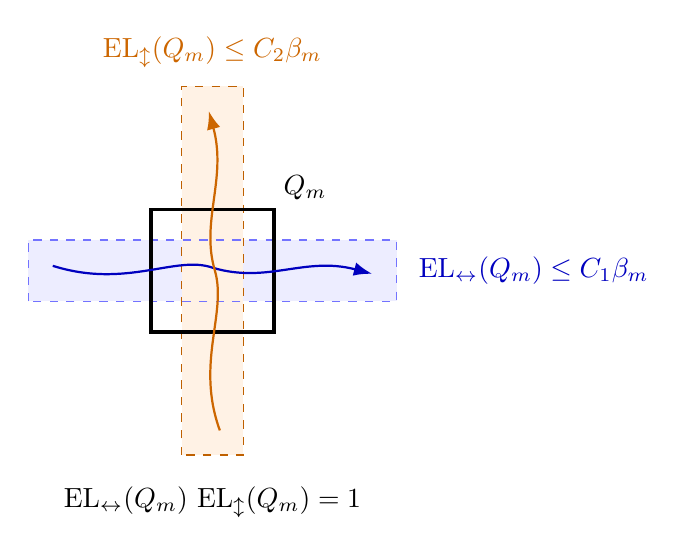
\begin{tikzpicture}[scale=.78,>=Latex]
  \fill[blue!7] (-3,-.5) rectangle (3,.5);
  \fill[orange!10] (-.5,-3) rectangle (.5,3);
  \draw[blue!55,dashed] (-3,-.5) rectangle (3,.5);
  \draw[orange!75!black,dashed] (-.5,-3) rectangle (.5,3);
  \draw[very thick] (-1,-1) rectangle (1,1);
  \node[anchor=south west] at (1,1) {$Q_m$};
  \draw[blue!75!black,thick,->]
       (-2.6,.08) .. controls (-1.4,-.3) and (-.6,.26) .. (0,.05)
                 .. controls (.9,-.22) and (1.5,.24) .. (2.6,-.05);
  \draw[orange!80!black,thick,->]
       (.12,-2.6) .. controls (-.28,-1.5) and (.24,-.7) .. (.04,0)
                 .. controls (-.2,.8) and (.24,1.5) .. (-.06,2.6);
  \node[anchor=west,text=blue!75!black] at (3.2,0)
       {$\EL_{\leftrightarrow}(Q_m)\le C_1\beta_m$};
  \node[anchor=south,text=orange!80!black] at (0,3.15)
       {$\EL_{\updownarrow}(Q_m)\le C_2\beta_m$};
  \node[anchor=north] at (0,-3.35)
       {$\EL_{\leftrightarrow}(Q_m)\,\EL_{\updownarrow}(Q_m)=1$};
\end{tikzpicture}

\caption{The dashed strips represent \(R_v(z,s)\) and
\(R_{v^\perp}(z,s)\).  Their strict lateral clearance forces
crossings of the corresponding sides of the common quadrilateral
\(Q_m\).  The picture uses the reference coordinate; the extremal lengths are those of the actual flag surface.
Finite bounds at one common radius contradict duality when
\(\beta_m\to0\).}
\label{conf:transverse-figure}
\end{figure}

\begin{proposition}[Macroscopic extremal-length bounds]
\label{conf:macroscopic-el}
In every diverging-scale extraction, including the finite sphere,
the following hold in the reference coordinate.
\begin{enumerate}
\item For every \(d>0\), the family of all discrete-surface paths
whose projected diameter is at least \(d\) has a positive limiting
lower extremal-length bound.
\item There is a deterministic \(c_*>0\) such that every fixed
round annulus \(A(z,r,2r)\) in an ordinary coordinate chart has
\[
 \liminf_n\EL_{X_n}\bigl(H_n^{-1}
                   \mathcal C_{\rm tr}(A(z,r,2r))\bigr)\ge c_*.
\]
The assertion holds simultaneously for a countable dense annulus
library, with strict margins.  It includes annuli surrounding an
isolated exceptional mark whose closures avoid the marks.
\end{enumerate}
\end{proposition}

\begin{proof}
Proposition~\ref{conf:no-degeneration} makes the high-probability
barriers uniformly positive in raw EL units. To pass from powers of four
to an arbitrary diverging integer sequence, write
$n=4^{j_n}v_n$, where $j_n=\lfloor\log_4 n\rfloor$ and $1\le v_n<4$,
and extract $v_n\to v\in[1,4]$ jointly with every fixed offset array.
Reexpress the same raw cuts and incidence readouts in the new units:
the area clock is divided by $v_n$, frontier heights by $\sqrt{v_n}$,
and the real field is shifted by $-\gamma^{-1}\log v_n$.
The actual flag-surface extremal length is unchanged. Strict chart
margins allow the converging factors to be retained through this
indexed-array identity. On each fixed buffered domain, the constant
shifts lie in a bounded family and admit cutoff extensions of uniformly
bounded Dirichlet norm. The two-sided Cameron--Martin comparison
therefore chooses a common high-probability barrier threshold before
annular alignment. This argument does not identify differently indexed
kernels at an unshifted field. Apply the aligned-annulus result and
Lemma~\ref{conf:density-budget} with \(\beta_m=1\).

For a curve making advance \(d\) compactly in \(U\), choose \(N\)
with \(CR_N<cd/4\).  The density charges the entire family by at
least \(cd/2\), for large \(m\), and has bounded energy.  Its
extremal length is therefore bounded below by a constant times
\(d^2/\Area(U^{+CR_N})\).  A finite collection of ordinary patches
catches a fixed positive subadvance of every curve of spherical
diameter at least \(d\).  To obtain such a collection, first remove
disjoint sufficiently small neighborhoods of the finitely many
exceptional marks; a curve of diameter \(d\) either makes an
advance away from them or crosses one of their surrounding compact
annuli.  Cover the resulting compact regions by finitely many
ordinary boxes and sum the densities.  This proves the first claim
for the entire family at once.

For a through crossing of \(A(z,r,2r)\), take a slightly larger
annular union of boxes of area at most \(Cr^2\).  Each crossing
makes projected advance at least a fixed multiple of \(r\) there.
The preceding quotient is bounded below by a universal constant.
The union can avoid the center and all other exceptional marks; in
particular this proves the assertion for fixed shells surrounding
an exceptional center.  Changes of ordinary field law preserve the
eventual statement and its constant.  Countable extraction handles
all rational tests and margins simultaneously. Lemma~\ref{ker:sphere-density}
transfers these probability-one conclusions to the finite sphere at its
actual area-normalized heights; Theorem~\ref{ker:local-kernels} retains
the same incidence and extremal-length readouts.
\end{proof}

\subsection{An all-center ring criterion}
\label{conf:analytic-subsection}

We give the analytic compactness statement in a form requiring no
estimate at a radius depending on \(n\).  In a finite conformal
atlas of the round sphere, fix the countable library of annuli
\(A(z,r,2r)\) with rational centers and radii and compact closure
in a chart.  Annuli around finitely many omitted centers are also
allowed, as in Proposition~\ref{conf:macroscopic-el}.

\begin{lemma}[Ring criterion]
\label{conf:ring-criterion}
Let \(f_n:\Chat\to\Chat\) be homeomorphisms.  Suppose that
\(f_n(z_n^i)=w_n^i\), where both triples converge to triples of
distinct points.  Suppose that, for every annulus \(A\) in the
preceding library,
\begin{equation}
 \liminf_n\EL_{\rm tr}(f_n(A))\ge c_*>0.
 \label{conf:ring-hypothesis}
\end{equation}
Then the maps and their inverses are equicontinuous.  Every
subsequential uniform limit is a \(K(c_*)\)-quasiconformal sphere
homeomorphism, with either orientation.
\end{lemma}

\begin{proof}
The two ring estimates below give equicontinuity and exclude collapsed
continua.  Annuli with shifted centers will then bound the linear
distortion of each limit.

\paragraph{Two ring estimates.}
Let \(E,F\) be the two
complementary continua of a sphere annulus.  If both have spherical
diameter at least \(u\), every essential closed curve in the annulus
has spherical length at least \(u/4\).  Otherwise its trace lies
in a disk of radius \(u/4\); each continuum has a point outside
that disk, so the curve is null-homotopic in the sphere minus those
two points, a contradiction.  Constant spherical density and
\eqref{conf:duality} give
\begin{equation}
 \EL_{\rm tr}(\Chat\setminus(E\cup F))
       \le 64\pi/u^2.
 \label{conf:ring-diameter-bound}
\end{equation}
If additionally \(d=\dist(E,F)\to0\) while both diameters stay
above \(u\), choose nearest points and center geodesic circles at
the point in \(E\).  For \(2d<t<u/4\), both continua meet the
circle of radius \(t\).  There is a circle arc joining them whose
interior is in the annulus.  Every admissible crossing density
therefore has integral at least one on that circle.  Cauchy--Schwarz
and polar integration imply
\begin{equation}
 \EL_{\rm tr}(\Chat\setminus(E\cup F))
       \le \frac{2\pi}{\log(u/(8d))}\longrightarrow0.
 \label{conf:ring-touching-bound}
\end{equation}
The density is extended by zero on the complementary continua when
performing this integration.

\paragraph{Equicontinuity and exclusion of collapsed continua.}
Fix \(\delta>0\) smaller than the pairwise limiting distances of
the target marks, and fix an image tolerance \(u>0\).  Choose
an integer \(k\) so large that
\(kc_*/2>64\pi/\min(u,\delta)^2\).  Around each source point
choose an outer coordinate disk omitting two limiting source marks
with clearance.  Inside it choose a stack of \(k\) rational
concentric annuli, with disjoint closures and a smaller central
disk.  Rational centers and radii can be chosen so that these
central disks cover the sphere; retain a finite subcover.  For this
finite collection, \eqref{conf:ring-hypothesis} gives a common
eventual index with all image moduli at least \(c_*/2\).  Series
addition and \eqref{conf:ring-diameter-bound} imply that every
retained central disk has image diameter less than \(u\): its
outer complementary continuum contains two target marks separated
by at least \(\delta\).  A Lebesgue number for the finite source
cover proves equicontinuity.  Only finitely many fixed annuli were
used for each \(u\).

Arzel\`a--Ascoli supplies a uniform limit \(f\), which is onto:
for each target point extract a convergent sequence of its
preimages.  Its fibers are connected.  Indeed, if a fiber split
into two disjoint nonempty compact sets, choose disjoint open
neighborhoods of these sets.  Their complement has image bounded
away from the fiber value.  For large \(n\), the connected
preimage under \(f_n\) of a sufficiently small disk about that
value would lie in the two neighborhoods and meet both, which is
impossible.

Suppose a fiber \(C\) is nontrivial.  Choose \(a\in\partial C\),
\(c\in C\setminus\{a\}\), and \(d\notin C\).  Take
\(b\notin C\) sufficiently close to \(a\).  A fixed rational
annulus can be chosen with \(a,b\) strictly inside its inner disk
and \(c,d\) strictly outside its outer disk.  The complementary
continua of its \(f_n\)-image have diameters bounded below by the
positive limiting distances from \(f(b)\) and \(f(d)\) to
\(f(a)=f(c)\), but their mutual distance tends to zero.  This
contradicts \eqref{conf:ring-touching-bound} and the lower bound
for this single fixed annulus.  Thus \(f\) is a homeomorphism.

\paragraph{Quasiconformality and inverse equicontinuity.}
We give the quantitative local criterion as well.  Work in finite
planar coordinates on a disk whose image avoids the target pole.
For a bounded planar annulus with through EL at least \(m>0\),
let \(e_0,e_1\) belong to its bounded complementary component and
\(w\) to the unbounded component.  The same circle integration
as above, with the unbounded continuum crossing every sufficiently
large circle, gives
\begin{equation}
 |w-e_i|\ge \theta(m)|e_1-e_0|\quad(i=0,1),
 \qquad \theta(m)=\tfrac12 e^{-2\pi/m}.
 \label{conf:relative-ring}
\end{equation}
For a fixed rational source annulus apply this with \(m=c_*/2\)
to \(f_n\), then pass to \(f\).  Approximation of centers,
radii, and points extends the inequalities to every sufficiently
small source annulus.  There is no common discrete threshold in
this approximation.

Put \(L(z,r)=\max_{|v-z|=r}|f(v)-f(z)|\) and define
\(l(z,r)\) by the corresponding minimum.  With
\(\theta=\theta(c_*/2)\), \eqref{conf:relative-ring} yields
\[
 l(z,2r)\ge\theta L(z,r).
\]
For \(|w-z|=2r\), let \(v=(z+w)/2\) and apply the same
inequality to the annulus centered at \(w\), where \(v\) lies
on its inner circle and \(z\) on its outer circle.  Provided
\(B(z,4r)\) is in the chart, this gives
\[
 |f(z)-f(v)|\ge\theta|f(v)-f(w)|,
 \qquad
 L(z,2r)\le(1+\theta^{-1})L(z,r).
\]
Consequently
\begin{equation}
 \frac{L(z,2r)}{l(z,2r)}
       \le \theta^{-1}(1+\theta^{-1}).
 \label{conf:linear-distortion}
\end{equation}
This is the metric criterion for planar quasiconformality
\cite[Theorem~1]{Cristea1989Quasiconformality}; see also
\cite[Theorem~2.5.3]{AstalaIwaniecMartin2009}. The
argument is precisely the lower-bound part of the proof of
\cite[Lemma~3.1, equations~(3.3)--(3.7)]{IvriiMarkovic2019}; the
shifted centers explain why one needs the all-center hypothesis.
One can also see the required Sobolev regularity directly:
\eqref{conf:linear-distortion} bounds \(L(z,r)^2\) by a constant
times \(\Area(f(B(z,r)))\).  Integrating squared coordinate
difference quotients, and using Fubini for the locally finite
measure \(V\mapsto\Area(f(V))\), gives bounded \(L^2\)
difference quotients on every compact subdomain.  Hence
\(f\in W^{1,2}_{\rm loc}\), and the metric criterion gives
bounded distortion.  Charts at the pole, or point removability,
finish the sphere assertion; a reflection handles the other
orientation.

Finally, failure of inverse equicontinuity would give target points
approaching one another whose source preimages stay separated.
Extract a uniform limit of the corresponding \(f_n\)'s and
convergent source preimages.  The limit would identify two distinct
points, contradicting the homeomorphism just proved.
\end{proof}

\subsection{The infinitesimal structure is round}
\label{conf:tensor-subsection}

The elimination of deterministic anisotropy by rotations has a parallel
in \cite[Section~4.4]{HoldenYuUniformization}, where determinism comes
from energy homogenization.  Here the conditional-product and field-germ
argument of Lemma~\ref{conf:germs} supplies that step.

\begin{lemma}[Conformal rigidity]
\label{conf:tensor}
Every homeomorphic limit in Lemma~\ref{conf:ring-criterion}, when
obtained from the local flag-surface arrays above, is conformal or
anticonformal.
\end{lemma}

\begin{proof}
Let \(f_n=\phi_n\circ H_n^{-1}\to f\) uniformly.  The image
of a local quadrilateral \(R\) has the same modulus as its actual
flag-surface preimage.  Strict inner and outer port versions
therefore determine the modulus of \(f(R)\): uniform convergence
of maps and inverses places the four sides between arbitrarily
small collars, with their marked sides in the correct order.
Conformal rectangle modulus is continuous under these Jordan
collar approximations.  The two transverse comparisons in
\eqref{conf:duality} supply the two sides of this determination.
Thus all these local moduli are readouts of the local EL arrays.
Global three-point normalization does not enter them, since
M\"obius postcomposition preserves modulus.

The distortion bound \eqref{conf:linear-distortion} implies that
\(f\) is differentiable almost everywhere
\cite[Lemma~2]{Cristea1989Quasiconformality}.  Its quasiconformality
also gives a nonzero Jacobian almost everywhere
\cite[Theorem~3.1.2]{AstalaIwaniecMartin2009}.
At a point \(z\) satisfying both conclusions put
\begin{equation}
 T(z)=\frac{Df(z)^{\mathsf T}Df(z)}{|\det Df(z)|}.
 \label{conf:tensor-definition}
\end{equation}
This positive symmetric tensor has determinant one and bounded
eccentricity.  It is a germ readout of the local moduli.  Here is
an explicit way to recover it.  For a unit vector \(v\) and
\(t>0\), let \(R_{v,t}\) have length one in direction \(v\)
and width \(t\).  Differentiability implies uniform convergence
of the rescaled images of \(z+rR_{v,t}\) to
\(Df(z)R_{v,t}\), for fixed \(t\).  If \(L\) is a nonsingular
linear map, constant density and straight-line flows give
\[
 \frac{(|Lv|-t|Lv^\perp|)_+^2}{t|\det L|}
 \le \EL_{\leftrightarrow}(LR_{v,t})
 \le \frac{|Lv|^2}{t|\det L|}.
\]
Multiplying by \(t\) and letting \(t\downarrow0\) recovers
\(v^{\mathsf T}T(z)v\).  Three fixed directions, with countable
sequences of \(r,t\) and strict covers, determine the tensor.
This proves both local readability and spatial measurability.

Lemma~\ref{conf:germs} makes \(T(z)\) deterministic for almost
every deterministic \(z\).  A coordinate rotation conjugates it
by the rotation matrix; the possible orientation sign of \(f\)
has disappeared from \eqref{conf:tensor-definition}.  Applying
the rotation part of that lemma to a quarter-turn gives
\(T=R^{\mathsf T}TR\).  For a symmetric two-by-two matrix this
sets the off-diagonal entries to zero and equates the diagonal
entries.  Since \(\det T=1\), we obtain \(T=I\) almost
everywhere.  The quasiconformal differential is therefore a
similarity almost everywhere, of one fixed orientation.  The
analytic characterization of quasiconformal maps
\cite[Theorem~2.5.4]{AstalaIwaniecMartin2009} makes \(f\)
conformal or anticonformal.  Isolated marked points are removable.
\end{proof}

\subsection{Actual marks, uniformization, and area}
\label{conf:normalization-subsection}

The remaining normalization uses the three fresh area samples of the
finite model.  We first record how these samples behave under the
reference homeomorphisms.

\begin{lemma}[Area marks under a converging coordinate]
\label{joint:marks}
Suppose $H_n:X_n\to\Chat$ are homeomorphisms and
$(H_n)_*m_n\Rightarrow\mu$ weakly, where $\mu$ is diffuse. Conditional
on the surface and exploration data used to choose $H_n$, let
$x_n^1,x_n^2,x_n^3$ be fresh independent samples from $m_n$. In
particular $H_n$ is chosen before these three marks. Then their images
converge jointly, together with the surface data, to three conditionally independent $\mu$ samples.
Almost surely these limiting points are distinct. The M\"obius map
sending the ordered triple to $0,1,\infty$ varies continuously with
the triple as long as the three points are distinct.
\end{lemma}

\begin{proof}
For continuous functions $f_1,f_2,f_3$ on $\Chat$, conditional
expectation of their product is
\[
 \EE\!\left[\prod_{j=1}^3 f_j(H_n(x_n^j))\,
        \middle|\,\text{surface data}\right]
   =\prod_{j=1}^3\int f_j\,\dd(H_n)_*m_n.
\]
Weak convergence passes the right side to
$\prod_j\int f_j\,\dd\mu$. Products of continuous test functions
determine the law on the compact product sphere, proving the joint
conditional assertion. Diffuseness gives distinctness. In a chart
avoiding the limiting points at infinity, the normalized M\"obius
map is the usual cross-ratio expression; its coefficients depend
continuously on the distinct triple. The resulting maps and their
inverses converge uniformly in spherical distance by compactness.
Other chart choices give the same conclusion when one point is
infinite.
\end{proof}

\begin{theorem}[Canonical uniformization comparison]
\label{conf:canonical}
Keep any joint extraction of the finite-map encoding and its local
observations.  Let \(x_n^1,x_n^2,x_n^3\) be the actual independent
\(m_n\)-samples used to define \(\phi_n\).  In the reference
coordinate these marks converge jointly to three conditionally
independent samples \(z^1,z^2,z^3\) of \(\mu_h\).  The maps
\(\phi_n\circ H_n^{-1}\) have uniformly convergent subsequences,
and every limit is the M\"obius or anti-M\"obius map taking
\((z^1,z^2,z^3)\) to \((0,1,\infty)\).  All retained local
observations use this same limiting coordinate and the same possible
orientation sign.
\end{theorem}

\begin{proof}
An original edge contributes four equal-mass flags and one
quadrangle.  Choosing a uniform quadrangle and then one of its
two matched tour steps gives a uniform step of the exploration.
By Proposition~\ref{top:projection} and Theorem~\ref{top:homeomorphism},
every point in any of its four
flags and either step representative have vanishing discrepancy
in the reference coordinate, uniformly over the map.  Hence, for
every continuous test function \(g\),
\[
 \int g\,\dd (H_n)_*m_n
       -\frac1{2n}\sum_{j=1}^{2n}g(\eta(j/(2n)))
       \longrightarrow0.
\]
The continuity of \(\eta\) and its quantum-area parameterization
identify the Riemann-sum limit as \(\int g\,\dd\mu_h\).
Repeated incidence labels cause no change: the four flags are
counted as occurrences.  Thus \((H_n)_*m_n\Rightarrow\mu_h\).

The maps \(H_n\) were chosen before the fresh samples.  Apply
Lemma~\ref{joint:marks} to this reference area convergence.  The
limiting marks have conditional law \(\mu_h^{\otimes3}\), jointly
with the retained map and local observations, and are almost surely
distinct.  Thus both the source marks and their prescribed target
images satisfy the normalization hypothesis of the ring criterion.

Conformal invariance identifies the through EL of
\((\phi_n\circ H_n^{-1})(A)\) with the actual surface EL for
the corresponding annulus.  Proposition~\ref{conf:macroscopic-el},
with strict collars, gives the hypothesis of
Lemma~\ref{conf:ring-criterion} simultaneously for the countable
annulus library.  That lemma gives uniform subsequential
convergence to a quasiconformal homeomorphism.  Lemma~\ref{conf:tensor}
makes it conformal or anticonformal, hence M\"obius or
anti-M\"obius on the sphere.  Uniform convergence and convergence
of the moving marks preserve their prescribed images.  These
three images specify the map once its orientation is fixed.
All extractions retained the same local arrays and topological
correspondence, so no observation acquires a different coordinate.
\end{proof}

\begin{corollary}[Canonical area and maximum mesh]
\label{conf:mesh-area}
In the joint coupling of Theorem~\ref{conf:canonical}, with
limiting normalization \(f\),
\[
 (\phi_n)_*m_n\Rightarrow f_*\mu_h,
 \qquad
 \max_T\diam_\rho\phi_n(T)\longrightarrow0.
\]
The measure on the right is the area of the quantum sphere in
the same three-marked coordinate; a common reflection is retained
when the correspondence reverses orientation.  In particular,
the maximum-mesh conclusion holds in probability along the full
sequence.
\end{corollary}

\begin{proof}
Write \(f_n=\phi_n\circ H_n^{-1}\).  Uniform convergence and
the reference area convergence prove the measure assertion.  If
\(\omega_f\) is a modulus of continuity of \(f\) on the sphere,
then
\[
 \max_T\diam_\rho\phi_n(T)
 \le2\|f_n-f\|_\infty+
       \omega_f\!\left(\max_T\diam_\rho H_n(T)\right)
       \longrightarrow0
\]
by \eqref{conf:topological-mesh}.  Every sequence has a further
joint extraction with these conclusions, which proves the stated
in-probability assertion about mesh.  The
three samples and \(\phi_n\) throughout are the prescribed
finite ones.
\end{proof}

\begin{corollary}[Area-typical root position]
\label{conf:root-area}
The exploration root has diffuse limiting area position in the
canonical coordinate.  This conditional sampling statement remains
valid jointly with any root-free map observations retained in the
same extraction.
\end{corollary}

\begin{proof}
Use the exact conditional rerooting statement in
Lemma~\ref{intro:root-flag}.  A uniform oriented-edge tail can be
coupled to a uniform flag by choosing one of its two sides, and
then to an independent uniform point of that flag.  The two
canonical positions differ by at most the maximum flag diameter.
Conditional on the root-free map data and the normalization
samples, this gives the same limiting continuous-test integrals
as sampling from \((\phi_n)_*m_n\).  Apply
Corollary~\ref{conf:mesh-area}.  The resulting area measure is
nonatomic.
\end{proof}

\section{The complete collection of interfaces}\label{loop:section}

We identify every macroscopic interface, including its traversal order
and its place in the nested collection.  Write $H_n:X_n\to\Chat$
for the homeomorphisms of the
topological correspondence and $\eta:[0,1]\to\Chat$ for the limiting
space-filling exploration, in the common coupling with the surface and
all retained observations.  In particular, $\eta(0)=\eta(1)=p_*$,
the images under $H_n$ of the flag triangles have maximum diameter tending
to zero, and the spatial representatives of the discrete tour converge
uniformly to $\eta$.  All the results of this section concern that
correspondence; the final coordinate change is made in
Proposition~\ref{loop:canonical}.

There are two steps.  Exact surgery on the finite exploration tour
represents each FK loop by a face of a noncrossing chord system.
Convergence of all these faces gives a complete collection of ordered
limiting curves, with no extra macroscopic loops.  We then identify
these curves with CLE.  Exploration switches first identify each curve
as a closed initial portion of a CLE traversal; a two-sided winding
test rules out any nonconstant omitted portion.

The loop readout follows Sheffield's exploration-tree construction of
CLE \cite{SheffieldExplorationTrees} and its realization through
imaginary-geometry flow and counterflow lines \cite{MillerSheffieldIGIV}.
The alternating nested exploration is also used in
\cite[Section~2.1.6]{AruHoldenPowellSunCritical}. Finite-volume contour and
cone-time convergence comes from \citet{GwynneSunFKIII}; the argument
here upgrades it to simultaneous ordered-curve convergence in the
canonical conformal embedding.

\subsection{Flexible orders as a closed chord system}

Let $\mathbb T=\R/\Z$, identified with the boundary of the closed unit disk
$\overline{\mathbb D}$ by $t\mapsto e^{2\pi it}$.  For $a,b\in\mathbb T$,
write $[a,b]_{\rm d}$ for the straight chord joining their images.  This
notation distinguishes a disk chord from an interval in exploration time.
A \emph{chord system} is a closed set of unordered endpoint pairs, including
all diagonal pairs.  Its underlying lamination is the union of its chords
and $\partial\mathbb D$.  Noncrossing means that two distinct chords have
disjoint relative interiors.  A \emph{face} is a connected component of the
complement of the lamination in $\mathbb D$; faces are open convex sets.

For the length-$2n$ word, fix the distinct occurrence times
\[
 t_k=\frac{k-1/2}{2n},\qquad 1\le k\le2n.
\]
Here $t_k$ labels the visit in the interior of the $k$th step of the
abstract medial tour.  It does not assert an exact scalar-chord identity
at the interpolated contour height.  For a flexible order at position
$j$, with matched burger at $i<j$, use the chord $[t_i,t_j]_{\rm d}$,
labelled by that burger's type.  Adjoin the diagonal pairs to obtain
$\mathcal E_n$.  Every letter belongs to at most one flexible pair,
so these chords have distinct endpoints, even for consecutive matched
letters.  This convention is needed for the exact face surgery below.
The adjacent-cut times used in the contour limit differ by at most
$1/(2n)$; their replacement by $t_i,t_j$ preserves all limiting
endpoint assertions.  Spatial tracking at these occurrence times
follows from tracking at adjacent cuts, continuity of $\eta$, and
the vanishing image diameter of the intervening flags.

For the limiting excursion $Z=(L,R)$, a backward cone interval is
\[
 [v(t),t],\qquad
 v(t)=\inf\{s<t:L(u)\ge L(t),\ R(u)\ge R(t)
                         \text{ for }u\in[s,t]\}.
\]
Here $t$ is required to admit at least one such interval of positive
length.  Away from the end convention, precisely one coordinate agrees
at its two endpoints; this coordinate labels the entrance wall.  We use
the corresponding burger-type label.  Let $\mathcal E$ consist of the
circular endpoint pairs of these intervals and all diagonal pairs.

\begin{lemma}[Joint convergence of the chord systems]\label{loop:chords}
The coupling may be chosen so that $\mathcal E_n\to\mathcal E$ in the
Hausdorff topology on unordered pairs of points of $\mathbb T$, jointly
with all previously retained observations.  Both systems are noncrossing.
For every convergent sequence of nondegenerate discrete chords whose
limiting endpoints have representatives $0<a<b<1$, the matched entrance
times converge to $v(b)=a$ and the labels eventually agree.  Every chord
of $\mathcal E$ is approximated by discrete chords.  The system
$\mathcal E$ is a measurable function of $Z$.
\end{lemma}

\begin{proof}
If flexible matches interlaced, say $i<i'<j<j'$, the burger at $i'$ would
still be available when the flexible order at $j$ takes the older burger
at $i$.  This contradicts freshness.  Thus the discrete chords are
noncrossing, and the same holds for their limits.

We use the full statement of Gwynne--Sun
\cite[Theorem~1.11]{GwynneSunFKIII}, with its time interval $[0,2]$ rescaled to
$[0,1]$.  The theorem is for the empty-reduced word at each positive
integer $n$ and each fixed inventory parameter in $(0,1/2)$.  Its second
assertion identifies all subsequential limits of flexible orders with
nonvanishing interval span; its third assertion gives convergence of both
entrance quantities and eventual agreement of the wall label.  Its fourth
assertion simultaneously approximates maximal cone intervals in every
rational-endpoint open interval containing a specified rational interior
mark.  These statements are stronger than uniform contour convergence.

Apply these assertions first at the adjacent-cut times of the cited
theorem.  The deterministic one-mesh bound just noted gives the same
endpoint limits and wall labels at our occurrence times.  In particular,
it gives the upper endpoint-pair limit.  To check the lower
limit explicitly, fix $[a,b]=[v(b),b]\Subset(0,1)$.  Choose open intervals
$I_k$ with rational endpoints, containing $[a,b]$, whose closures decrease
to $[a,b]$, and fix a rational point of $(a,b)$.  The maximal cone interval
in $I_k$ containing that point contains $[a,b]$: cone intervals containing
the same interior point are ordered by inclusion.  Its endpoints
therefore tend to $a,b$.  For each $k$ the distinguished discrete maximal
intervals converge by the cited theorem.  A diagonal choice approximates
$[a,b]$.  Equivalently, first apply the theorem simultaneously to the
countable family of rational tests and then take their closure.  Compactness
of the endpoint-pair space turns the upper and lower conditions into
Hausdorff convergence.

There is no additional nondegenerate circular chord at an excursion end.
For example, a sequence with one endpoint tending to $0$ and the other
tending to an interior time would force an interior coordinate value to
be zero.  A sequence ending at $1$ with its entrance bounded away from $0$
would do the same, using equality in the entrance-wall coordinate.  Both
contradict strict interior positivity.  The sole possible full-duration
interval has equal endpoints on $\mathbb T$ and is already included among
the diagonal pairs.  The resulting closed chord system is determined by
the excursion.  Hence retaining it causes no ambiguity in the joint
subsequential couplings: its limiting conditional law given the excursion
is a point mass.
\end{proof}

\subsection{The exact finite surgery}

Let $\mathcal L_n$ be the lamination underlying $\mathcal E_n$.  A face
boundary can be read cyclically by following the time circle on its
exposed arcs and using its chord sides to skip the intervening intervals.
The circle here records the resolved-tree medial tour, not a second
conformal embedding of the map.

The resolved spanning tree has a disk as a small regular neighborhood.
Its boundary is the simple medial tour $C_n$; the complementary disk
is the dual-tree side.  The two marked visits associated with a flexible
pair lie in the two exploration triangles of one edge quadrangle.
The occurrence times fixed above place each mark inside its own visit.
Sliding a mark within that visit leaves the four-port pairing unchanged.

\begin{lemma}[Flag drawing and face surgery]\label{loop:surgery}
The faces of $\mathcal L_n$ are in bijection with the polygonal FK loops
specified in the model.  Under this bijection, the exposed time-circle
arcs give their cyclic tour order.  A transit along a chord changes the
spatial route only within its matched edge quadrangle, with an adjacent
tour-step error at its endpoints.

Suppose a face is entered across an outer chord with interval $[a,b]$ and
has an immediate child chord with interval $[c,d]\subset(a,b)$.  A test
point on the tour strictly inside $(c,d)$ lies on the opposite side of the
face loop from a test point on the outside time arc if and only if the
outer and child chord labels differ.  This assertion is made with test
points off the surgery quadrangles, or after taking arbitrarily small
strict spatial margins.
\end{lemma}

\begin{proof}
In an unoccupied flag triangle the retained corner is cut off by
$v=2/3$.  In an occupied triangle that corner is already contained in the
strip $f\le1/3$, and the boundary is $f=1/3$.  On a common
vertex--face-center side these two rules meet at the same point.  On the
other two side types the occurrences are paired within the same edge
quadrangle and have the same occupation status.  Consequently the four
ports of an edge quadrangle have exactly the usual two FK pairings.
They are shown in Figure~\ref{enc:flag-quadrangle}.
This verification is occurrence by occurrence, so loops and bridges do
not identify distinct ports accidentally.

Starting from $C_n$, restore the FK pairing at each flexible quadrangle.
Cut its two marked visits and reconnect the four cut ends by the other
noncrossing pairing.  In the abstract disk this is a cut along
$[t_i,t_j]_{\rm d}$.  Noninterlacing ensures that the chord lies in one
current face, and its distinct endpoints divide that face into two.
Induction therefore identifies the final cyclic routes with all disk
faces, giving $1+N_{\mathsf F}$ of each.  Each reconnection stays in its
own quadrangle.  The polygonal flag drawing has the same four-port
pairings, so it has exactly these cyclic routes in the exposed
time-circle order.  This argument retains even the smallest finite
loops; it does not replace a chord between consecutive occurrences by
a diagonal pair.

For the side assertion, realize each switch by a narrow bridge in the
disk on the side of its resolved-tree edge.  The two burger types use
the two opposite disks of $C_n$.  Within either disk the bridges may
be chosen disjoint because their endpoints do not interlace.
Fix an outer bridge with interval $[a,b]$, its child bridge $[c,d]$,
and a reference point on $C_n(b,a)$.  If the bridges use the same disk,
the face route bounds the strip between them.  The skipped arc
$C_n(c,d)$ and the reference arc $C_n(b,a)$ lie on the same side of
this route.  If the child bridge uses the other disk, the skipped arc
$C_n(c,d)$ lies between that bridge and the outer bridge, while the
reference arc remains on the other side.  Thus the two test points
are separated exactly when the bridge types differ; see
Figure~\ref{loop:surgery-sides-figure}.  Subsequent reconnections are
disjoint from this face route and cannot change either test point's
component.  This proves the criterion.  The
same conclusion can be checked directly from the detailed component
identification in \cite[Lemmas~2.7 and~2.9]{GwynneMaoSunFKI}.
\end{proof}

\begin{figure}[ht]
\centering
\begingroup
\definecolor{loopsideroute}{RGB}{28,79,114}
\definecolor{loopsidefill}{RGB}{226,240,246}
\begin{tikzpicture}[x=1cm,y=1cm,font=\small,
  tour/.style={draw=black!55,densely dashed,line width=.65pt},
  route/.style={draw=loopsideroute,line width=1.25pt},
  arcname/.style={font=\scriptsize,fill=white,inner sep=1.5pt},
  bridge/.style={font=\scriptsize,text=loopsideroute,inner sep=1pt},
  leader/.style={draw=black!45,line width=.4pt},
  testpoint/.style={circle,fill=black,inner sep=1.35pt}]

  \foreach \shift/\case in {0/0,7.15/1}{
    \begin{scope}[xshift=\shift cm]
      \coordinate (a) at (150:1.8);
      \coordinate (c) at (110:1.8);
      \coordinate (d) at (70:1.8);
      \coordinate (b) at (30:1.8);

      \ifnum\case=0
        \path[fill=loopsidefill]
          (a) arc[start angle=150,end angle=110,radius=1.8]
          .. controls (-.40,.60) and (.40,.60) .. (d)
          arc[start angle=70,end angle=30,radius=1.8]
          .. controls (1.10,-.30) and (-1.10,-.30) .. cycle;
      \else
        \path[fill=loopsidefill]
          (a) arc[start angle=150,end angle=110,radius=1.8]
          .. controls (-.90,2.80) and (.90,2.80) .. (d)
          arc[start angle=70,end angle=30,radius=1.8]
          .. controls (1.10,-.30) and (-1.10,-.30) .. cycle;
      \fi

      \draw[tour] (0,0) circle (1.8);
      \node at (-.76,-1.06) {$D_{\rm p}$};
      \node at (2.15,-1.08) {$D_{\rm d}$};

      \draw[route] (a)
        arc[start angle=150,end angle=110,radius=1.8];
      \draw[route] (d)
        arc[start angle=70,end angle=30,radius=1.8];
      \draw[route] (b)
        .. controls (1.10,-.30) and (-1.10,-.30) .. (a);
      \node[bridge] at (0,-.30) {outer bridge in $D_{\rm p}$};

      \ifnum\case=0
        \draw[route] (c)
          .. controls (-.40,.60) and (.40,.60) .. (d);
        \node[bridge] at (0,.55) {child in $D_{\rm p}$};
        \node[font=\small\bfseries] at (0,3.17)
          {(a) Same bridge side};
        \node[align=center,font=\small] at (0,-2.70)
          {$p$ and $r$ are in the same component};
      \else
        \draw[route] (c)
          .. controls (-.90,2.80) and (.90,2.80) .. (d);
        \node[bridge] at (0,2.78) {child in $D_{\rm d}$};
        \node[font=\small\bfseries] at (0,3.17)
          {(b) Opposite bridge sides};
        \node[align=center,font=\small] at (0,-2.70)
          {$p$ and $r$ are in opposite components};
      \fi

      \draw[leader] (-2.00,1.53) -- (130:1.8);
      \node[arcname] at (-2.28,1.60) {$C(a,c)$};
      \draw[leader] (2.00,1.53) -- (50:1.8);
      \node[arcname] at (2.28,1.60) {$C(d,b)$};
      \draw[leader] (-.10,1.96) -- (96:1.8);
      \node[arcname] at (0,2.08) {$C(c,d)$};
      \node[arcname] at (0,-2.16) {$C(b,a)$};

      \foreach \point/\place in {a/below left,c/above left,
                                  d/above right,b/below right}{
        \fill[loopsideroute] (\point) circle (1.15pt);
        \node[\place,inner sep=2pt] at (\point) {$\point$};
      }
      \node[testpoint,label={[inner sep=3pt]right:$p$}] at (0,1.8) {};
      \node[testpoint,label={[inner sep=3pt]right:$r$}] at (0,-1.8) {};
      \node[font=\scriptsize,text=black!70] at (0,-1.53)
        {outside reference};
    \end{scope}
  }

  \draw[route] (-2.52,-3.35) -- (-1.88,-3.35);
  \node[anchor=west,font=\scriptsize] at (-1.73,-3.35)
    {face loop};
  \draw[tour] (1.12,-3.35) -- (1.76,-3.35);
  \node[anchor=west,font=\scriptsize] at (1.91,-3.35)
    {skipped arcs of $C$};
  \path[fill=loopsidefill,draw=loopsideroute!50,line width=.4pt]
    (5.49,-3.45) rectangle (5.91,-3.25);
  \node[anchor=west,font=\scriptsize] at (6.06,-3.35)
    {one complementary component};
\end{tikzpicture}
\endgroup

\caption{The side test for an outer switch $[a,b]$ and its child
$[c,d]$.  The circle is the spatial resolved-tree tour $C$, separating
the primal and dual disks $D_{\rm p},D_{\rm d}$.  A point $p$ on
the skipped child arc lies with the exterior reference point $r$
exactly when both bridges use the same disk.  The bridge curves
represent narrow surgery strips in a topological drawing; their
lengths do not represent distances in the flag triangles.}
\label{loop:surgery-sides-figure}
\end{figure}

\begin{remark}\label{loop:count}
The finite drawing is a regular neighborhood of $(V(M_n),A_n)$.
If it has $k(A_n)$ components and $b_n$ boundary loops, its Euler
characteristic is both $|V(M_n)|-|A_n|$ and $2k(A_n)-b_n$.  Hence
$b_n=2k(A_n)+|A_n|-|V(M_n)|=\ell(M_n,A_n)$.  The surgery description
likewise gives one plus the number of flexible orders.  Thus the face
bijection counts the actual interfaces of the specified ensemble.
\end{remark}

\subsection{From chord convergence to complete loop matching}

Let $\mathcal L$ be the lamination underlying $\mathcal E$.  For a chord
with endpoints $a,b$, the peanosphere identification gives
$\eta(a)=\eta(b)$.  Thus there is a map
\[
 Q:\mathcal L\longrightarrow\Chat,
 \qquad Q(e^{2\pi it})=\eta(t),
 \qquad Q\big|_{[a,b]_{\rm d}}\equiv\eta(a).
\]
It is well defined and continuous.  To see continuity, consider a
convergent sequence of points on chords and extract convergent endpoint
pairs.  At a limit point in the open disk the limiting chord fixes the
value.  At a limit point of the time circle, strict convexity of the disk
forces that point to be an endpoint of the limiting chord, so the same
conclusion follows from $\eta(a)=\eta(b)$ and continuity of $\eta$.
For a face $F$ of $\mathcal L$, define $\ell_F$ to be the cyclic curve
$Q|_{\partial F}$.  Constant curves will be discarded.

We state the compactness argument in a form that also controls loops
whose indexing face varies with $n$.

\begin{lemma}[Convex cells and cyclic curves]\label{loop:convex}
In the common spatial correspondence the following assertions hold.
\begin{enumerate}
\item For every face $F$ of $\mathcal L$ and every $x\in F$, eventually
there is a unique face $F_n$ containing $x$, and
$\overline F_n\to\overline F$ in Hausdorff distance.  The associated
spatial FK loops converge to $\ell_F$ in uniform distance modulo cyclic
increasing reparameterization.
\item If $F_{n_j}$ is any sequence of faces, then after further extraction
$\overline F_{n_j}$ has a compact convex limit $K$.  If $K$ has interior,
it is the closure of one face of $\mathcal L$ and the corresponding
spatial loops converge cyclically to that face loop.  If $K$ has no
interior, the spatial loop diameters tend to zero.
\item The multiset of nonconstant $\ell_F$ is locally finite on the sphere.
For every $\varepsilon>0$, eventually there is a partial bijection between
the discrete and limiting face loops which covers every loop of spherical
diameter greater than $\varepsilon$, and each matched pair is at
individual-loop distance at most $\varepsilon$.
\end{enumerate}
\end{lemma}

\begin{proof}
Chord endpoint convergence implies Hausdorff convergence of the underlying
laminations.  A compact connected subset of $F$ has positive distance
from $\mathcal L$ and therefore lies in one discrete face eventually.
Exhausting $F$ by such compact subsets gives
$\overline F\subset\liminf\overline F_n$.  Every boundary chord of $F$
is approximated by discrete chords, and $F_n$ lies on the side of each
approximating chord selected by $x$.  The intersection of these closed
half-disks is $\overline F$.  This gives the reverse inclusion and proves
the first cell assertion.

For a varying sequence, compactness of the space of compact convex
subsets of $\overline{\mathbb D}$ gives a limit $K$.  If $K$ has interior,
no limiting chord can cut that interior: an approximating chord would
cut the corresponding discrete face.  Choose an interior point of $K$
outside the lamination.  The first part then identifies $K$ with a face
closure.  Such a point exists, since otherwise the lamination would
contain an open disk in $K$; a chord through that disk would again cut
$K$, which is impossible.

For the curve assertion in this case, parameterize $\partial F_n$ and
$\partial F$ by radial bearings from a fixed interior mark.  Their radial
functions converge uniformly.  Indeed an interior disk about the mark is
contained in all sufficiently large $F_n$, and convexity then bounds the
radial modulus uniformly; pointwise convergence follows from the cell
convergence.  These boundary parameterizations preserve cyclic order.
On exposed circle arcs, the spatial routes converge to $\eta$ uniformly.
On a chord side, Lemma~\ref{loop:surgery} confines the route to a matched
quadrangle, whose image diameter tends to zero.  Every subsequential
limit of such a route is therefore the common endpoint value of $Q$.
The compactness argument used above to prove continuity of $Q$ makes this
convergence uniform on the parameter circle.  Pauses inserted at chord
endpoints are harmless: continuous nondecreasing changes of time are
uniform limits of strictly increasing changes of time and give the same
zero-distance class in the stated loop topology.

Suppose instead that $K$ has no interior.  It is a point or a line
segment.  A closed convex cell is the convex hull of its contacts with
$\partial\mathbb D$.  Extracting those compact contact sets shows that
$K$ is the convex hull of its limiting circle contacts.  There are at most
two such contacts, since three distinct points of the circle are
noncollinear.  In the two-contact case, a boundary chord of a discrete
cell converges to their connecting segment.  For clarity, take a point
strictly between the two contacts and boundary points on either side of
it tending to the segment; these points are on chord sides, and any
limiting side through an interior point of the segment has exactly those
two circle endpoints.  The endpoints consequently have equal $Q$ values.
All exposed-circle route values and all chord-side route values have that
same subsequential limit.  Thus the spatial diameters tend to zero.

To prove local finiteness, suppose distinct limiting faces had loop
diameters bounded below.  Their closures have a subsequential convex
limit.  The preceding collapsed-cell argument, applied with the fixed
lamination, rules out an empty interior.  If the limit has interior, an
interior disk is eventually contained in every face in that subsequence,
contradicting disjointness of distinct faces.  Thus only finitely many
limiting face loops have diameter above any positive threshold.

Fix $\varepsilon>0$.  Match all limiting face loops of diameter greater
than $\varepsilon/2$ to the discrete faces selected by their interior
marks.  There are finitely many, their selected faces are distinct for
large $n$, and their cyclic errors tend to zero.  If unmatched discrete
loops of diameter greater than $\varepsilon$ remained along a subsequence,
Part~2 would produce a noncollapsed limiting face loop of diameter at
least $\varepsilon$.  Its interior mark would eventually belong to the
unmatched discrete face, contrary to the selected matching.  This proves
the final assertion, and a diagonal sequence of $\varepsilon$ gives the
claimed loop-ensemble topology.
\end{proof}

\subsection{The alternating exploration convention}

We now identify the limiting curves.  Put the exploration root at
$\infty$, and adjoin independent uniform times $U_1,U_2,\ldots$.
Their images $z_j=\eta(U_j)$ are area-typical targets.  Almost surely
these times are dense, the targets are dense in the sphere, and they
avoid all CLE loop traces.  We work on
one event on which the assertions below hold for all these targets and
all rationally truncated exploration windows.
Indeed the countable construction of the CLE loops and the frontiers
at rational times in a smooth spherical-area parameterization
are determined before the independent quantum field is sampled.
Their traces have zero Lebesgue area and consequently zero quantum
area almost surely.  A multiply visited point lies on such a frontier
between two of its visits.  Thus typical targets also have unique
visit times.

The exploration tree is the one determined by the imaginary field in
Section~\ref{local:section}.  Its branch toward $z_j$ is obtained from the
space-filling curve by erasing the fillings disconnected from $z_j$.
After a strict initial cut it is radial
$\mathrm{SLE}_{\kappa}(\kappa-6)$ in its target component.  The marked
boundary prime end and the growing tip have angular separation
$\theta\in[0,2\pi]$.  We use the following convention for extracting
\emph{nested} CLE from this tree: traverse a full excursion of $\theta$
from one endpoint of $[0,2\pi]$ to the other, complete its loop by the
branch aimed at the excursion's starting point, and repeat in the
remaining target component.  The completing branch approaches the
later prime-end lift of that point from the component separated from
the target at the end of the excursion.  This is the approach which
makes the starting point its terminal second visit
\cite[Section~2.1.6 and Figure~4]{AruHoldenPowellSunCritical}.
The directions alternate.  This precise
iteration is described in
\cite[Remark~2.3 and Sections~2.1.6--2.1.7]{AruHoldenPowellSunCritical}.
The whole-plane branching construction is that of
\cite[Section~2.3.1]{GwynneMillerQianCLE}; its whole-plane and local
radial laws are those of \cite[Section~2.1.3]{MillerSheffieldIGIV}.

\begin{lemma}[The unmarked law of the alternating construction]
\label{loop:ensemble-law}
The ensemble obtained by this alternating construction from the
whole-plane tree has the law of whole-plane $\mathrm{CLE}_{\kappa}$.
It is locally finite, its loops do not trace themselves or each other,
and its unmarked law is invariant under M\"obius transformations.
\end{lemma}

\begin{proof}
First consider a radial branching tree in a proper simply connected
domain $D$, with force point immediately on either side of its boundary
root.  The alternating construction is the nested-domain construction
of \cite[Section~2.1.6]{AruHoldenPowellSunCritical}.  Its first full
crossing, completed through the separated component, gives an outermost
loop.  The component of its complement containing a target is exactly
the radial target component at the crossing time.  Conditional on the
explored branches and completions, the unexplored trees in the
components are independent radial trees.  At the next generation the
force side is reversed, as follows from $\theta\mapsto2\pi-\theta$
and the strong Markov property
\cite[Remark~2.3]{AruHoldenPowellSunCritical}.  Reflection preserves the
unmarked domain CLE law.  Induction for finitely many targets and
generations, followed by the countable union, therefore gives the
independent-domain iteration defining nested $\mathrm{CLE}_{\kappa}$.
This also gives consistency at a discovered interior bubble: its
descendant loops are exactly those of the continued tree in that bubble,
and other loops of the domain ensemble cannot enter its interior.
Thus the two crossing directions give consecutive generations in this
construction.

We pass to the whole plane using stopping domains.  Choose a
deterministic target, put it at $0$, and use the bi-infinite Loewner
time of its branch from $\infty$.  Define
\[
 S_m=\inf\{t\ge -m:\theta(t)\in\{0,2\pi\}\},\qquad
 T_m=\inf\{t\ge S_m:\theta(t)=2\pi-\theta(S_m)\}.
\]
These are stopping times.  Full angular crossings occur arbitrarily
far toward the initial end
\cite[Lemma~2.7]{GwynneMillerQianCLE}, so $T_m\to-\infty$ almost
surely.  Explicitly, fix any earlier full crossing.  Once $-m$ precedes
its starting endpoint visit, $T_m$ is no later than its ending visit:
whichever endpoint is hit first after $-m$, both endpoints have been
visited by then.

Let $D_m$ be the component containing $0$ after $T_m$.  The tip and
force prime end coincide in the endpoint state $\theta(T_m)$.
The whole-plane strong Markov property and conditional
independence of branches after target separation imply that the
unexplored tree in $D_m$, conditionally on the exposed branch, is a
radial branching tree with the indicated endpoint force side
\cite[Proposition~2.2 and Section~2.1.3]{MillerSheffieldIGIV}.
The preceding domain argument shows that its future ensemble
$\Gamma^{(m)}$ has conditional law $\mathrm{CLE}_{\kappa}$ in $D_m$.
Its curves lie in $\overline D_m$ and may touch $\partial D_m$.

We check consistency with the global readout using only these domain
ensembles.  Fix a globally generated loop $G$ with target $w$ and a
finite starting crossing.  For sufficiently large $k$, the cut $T_k$
precedes both the separation of $w$ from $0$ and that crossing.  Then
$w\in D_k$, its branch shares the exposed prefix, and $G$ is a loop
of $\Gamma^{(k)}$: every subsequent full crossing and its completion
are computed from the same restricted tree.  Increase $k$ so that
$T_k<T_m$ as well.  In the domain construction for $\Gamma^{(k)}$,
$T_m$ is a later full-crossing time toward $0$, and $D_m$ is the
corresponding interior bubble.  Domain consistency therefore says
that $G$, if its trace enters $D_m$, is a descendant loop generated by
the continued tree there, hence belongs to $\Gamma^{(m)}$.
Conversely every loop of $\Gamma^{(m)}$ is a global crossing loop.
There are countably many cuts and generated loops, so these statements
hold simultaneously.  In particular the global and future readouts
agree on all loop tests in a compact subset of $D_m$, including loops
which touch $\partial D_m$ elsewhere.

The branch tends to $\infty$ at its initial end.  Thus every fixed disk
lies in $D_m$ eventually: for sufficiently negative $T_m$ the entire
exposed past lies outside that disk, whose connected interior belongs
to the $0$-component.  The domain limit theorem
\cite[Theorem~A.1]{MillerWatsonWilsonNestingField} identifies the limit
of $\mathrm{CLE}_{\kappa}$ in such domains with the unique whole-plane
law.  Its conformal matching estimate is uniform over all proper simply
connected domains, with error tending to zero as their boundary recedes
from a fixed disk.  It applies conditionally to $D_m$: bounded
continuous tests of the loop configurations in a fixed compact set
converge to the fixed whole-plane expectation, and dominated convergence
removes the conditioning.  The local agreement just proved identifies
the global alternating readout with this limit.  It also transfers
local finiteness and the absence of shared arcs directly from a domain
ensemble, since every compact set is eventually inside some $D_m$.

The whole-plane construction in \cite[Section~2.3.2]{GwynneMillerQianCLE}
uses a positive-crossing subsequence.  Its agreement in law with this
same large-domain limit is stated in Remark~2.6 of that paper.
Consequently its M\"obius-invariance theorem
\cite[Theorem~1.1]{GwynneMillerQianCLE} applies to the present unmarked
ensemble.
\end{proof}

We use no tracing in the strong sense of
\cite[Definitions~2.4--2.5]{GwynneMillerQianCLE}: no nonconstant
open portion of a traversal has its image contained in the union of
the complementary trace and the traces of finitely many other loops.  Reference
CLE traversals are parameterized without constant intervals; pauses
will be allowed when comparing them with face contours.  This
image-containment statement, rather than merely the absence of an
identical parameterized subarc, will be needed below.

The next dictionary relates three orders.  The interval $[a,b]$ uses
the quantum-area time of the space-filling curve: $a$ enters a filled
bubble and $b$ completes it.  Along a target branch, larger enclosing
intervals are encountered first.  Its moving clock erases the off-target
fillings while retaining the ordered branch trace.  The two endpoints
of a full angular crossing in branch time will be denoted by
$\sigma,\tau$; they need not be the area times $a,b$.

\begin{lemma}[Cone intervals and exploration switches]
\label{loop:switches}
For each typical target time $u$, the cone intervals containing $u$
describe the successively filled target bubbles.  Their order along the
branch toward $\eta(u)$ is reverse inclusion.  Their entrance-wall labels
are the two endpoint states of $\theta$, up to a fixed interchange.
Consequently a last closure of one type before a closure of the other
type starts the between-tips portion of a nested CLE loop.  The tree
completes that loop inside the larger interval's filling.

These switches recover all loops surrounding the target, once each.
Every typical target surrounded by such a completed loop belongs to its
outer interval's filling.  Enclosing cone intervals approach the full
time interval at the root end, and arbitrarily small such intervals
contain $u$.

For every fixed strict interior horizon, ancestor-free erasure has a
continuous moving trace.  In every nonempty interval of its moving
clock, erased intervals of both entrance-wall types occur.
\end{lemma}

\begin{proof}
We give the frontier dictionary in the cut surface, where different
prime ends over one spatial point remain distinct.  Color the left
side of the branch red and its right side blue.  The boundary of its
current target component consists, in prime-end order, of a red arc
and a blue arc between the tip $W$ and the marked junction $O$.
These are the boundary colors and exploration order of
\cite[Section~2.1.7 and Figure~9]{AruHoldenPowellSunCritical}.
The force prime end is precisely this junction $O$: it is transported
by the Loewner map until a collision, and the same boundary-color rule
continues it after the collision.  The two prime-end arcs have strictly
positive quantum length when they are nontrivial.  Therefore one color
is absent exactly when $O$ and $W$ coincide on the corresponding side,
that is, when $\theta=0$ or $\theta=2\pi$.

We use the precise bubble readout of
\cite[Section~2.3.4, Definition~2.2 and Figure~4; Lemma~3.1]
{GwynneMillerSLECharacterization}: a filled bubble has interval
$[v(b),b]$, its boundary length is $|Z(b)-Z(v(b))|$, and its side
is specified by the coordinate equal at the two endpoints.  This
statement uses backward cone intervals, with the same entrance
convention as here.  The following frontier verification explains
its use on the sphere.  When a
monocolored component is entered at time $a$, the space-filling order
visits all its descendants before returning to a different component;
write $b$ for its completion time.  Its interior is visited only during
this block, although its boundary points may be visited again.
The frontier outside this component
is unchanged throughout its filling.  Subtracting its terminal heights
therefore gives the two remaining frontier lengths
\begin{equation}\label{loop:frontier-lengths}
 \bigl(L(s)-L(b),\ R(s)-R(b)\bigr),\qquad a\le s\le b.
\end{equation}
They are nonnegative, both are zero at $b$, and exactly one is zero
at $a$.  The first entry $a$ is the entrance $v(b)$: in the
running-minimum frontier construction of
Theorem~\ref{enc:peanosphere}, extending the block farther backwards
crosses one of its two terminal frontier levels.

The converse uses the same frontier construction.  For a cone interval
$[v(b),b]$, cut the two frontier trees at heights $L(b)$ and $R(b)$
and retain its filling block.  The horizontal identifications inside
the block stay above those cuts.  Its unfilled boundary arcs are
parameterized by the height intervals in
\eqref{loop:frontier-lengths}; at its first time the arc for the
entrance wall is empty.  Maximality of $v(b)$ prevents a preceding
block from remaining on these same two sides of the cuts.  Thus this
is exactly the monocolored component entered there.  If the interval
contains $u$, it is the branch's target component, since its interior
contains $\eta(u)$; if it precedes $u$, it is an erased off-target
filling.  This verifies both directions of the readout without imposing
a new law on the field inside the component.  Erasing earlier
off-target fillings does not change these two boundary arcs in the
target component.  The argument concerns the restricted quotient and
its length coordinates on $[a,b]\Subset(0,1)$, which are the same
in the sphere realization of Theorem~\ref{enc:peanosphere}; no
infinite-volume surface law is being assigned to that block.

Combining \eqref{loop:frontier-lengths} with the prime-end description
identifies the entrance-wall labels with the two endpoint states of
$\theta$, up to interchanging the colors.  Target components shrink
along a branch, and their contiguous filling blocks are consequently
ordered by reverse inclusion.  The exact backward-cone erasure for a
target branch is also stated in
\cite[Section~4.2 and Definition~4.14]{AruHoldenPowellSunCritical};
the ancestor-free construction underlying it is
\cite[Proposition~1.13 and Lemma~10.4]{DMSMating}.

Starting at either state, the last visit to it before reaching the other
is the beginning of a full crossing of $[0,2\pi]$.  The alternating
constructor therefore gives precisely the stated switches and their
between-tips portions.  Conditional on that portion, the remaining
piece is chordal SLE in the specified prime-end component, as in
\cite[Section~2.1.6]{AruHoldenPowellSunCritical} and
\cite[Section~2.3.2]{GwynneMillerQianCLE}.  More precisely, let
$\sigma,\tau$ be the starting and ending branch times of the full
crossing, and view the target bubble at $\sigma$ in its prime-end disk.
The tip and force point coincide at its designated boundary root $x$.
The completing branch approaches the later lift of this same $x$
through the component separated from the target at $\tau$.  The
excursion and completion therefore give a closed continuous curve
$\beta$ in the closed prime-end disk, starting and ending at $x$.
Both pieces lie in the larger cone interval's filling.

Let $f$ map that disk to the outer bubble.  Its continuous extension
exists because the boundary is locally connected.  The closed curves
$f((1-\varepsilon)\beta)$ lie in the bubble and converge uniformly to
the completed loop as $\varepsilon\downarrow0$.  Simple connectedness
gives zero winding about every point outside the bubble for each
approximant.  Winding stability gives the same assertion for the
completed loop at every off-trace point outside the bubble.  Thus every
surrounded typical target is in that bubble.

Iteration supplies exactly the successive nested loops about a target.
Their domains decrease to that target.  In the whole-plane version they
also exhaust toward the initial point.  Equivalently, the full crossings
of the recurrent angular diffusion occur at all scales; the whole-plane
branch is transient at its initial end and tends to its target at its
terminal end.  For any fixed compact subinterval of $(0,1)$, large
enclosing bubbles contain its image.  Their fillings therefore contain
that time subinterval, and their endpoints tend to $0,1$.

Finally, for the unconditioned Brownian contour, the two boundary
processes after ancestor-free erasure, read in forward branch order,
have negative jumps and stable index
$\kappa/4\in(1,2)$, one for each side
\cite[Proposition~1.13]{DMSMating}.  This reverses the time direction
of the positive-jump processes in that statement.  Each L\'evy measure has
infinite mass near zero, so each coordinate has jumps in every nonempty
clock interval.  The jumps are precisely the erased cone intervals of
the indicated wall type.  The time-changed trace is continuous directly:
every inverse-clock jump skips an interval $[a,b]$ with
$\eta(a)=\eta(b)$, and $\eta$ is continuous.  This is the inverse-clock
argument in \cite[Proposition~10.6]{DMSMating}.
The erasure retains the full ordered branch traversal; the skipped
intervals are space-filling visits to off-target bubbles, not moving
pieces of that branch.  Thus a portion on which the branch changes
position occupies a nonempty interval of its moving clock.
For the excursion, exhaust by strict interior rational windows
containing the full Brownian-time span of the tested clock interval,
including all its erased intervals.  Local absolute continuity
transfers the null event that one label is missing there.  Taking the
countable intersection gives the assertion for rational and independent
uniform horizons.  Only this almost-sure property is transferred;
the excursion's time-changed coordinates need not be L\'evy processes.
\end{proof}

\subsection{Ordered prefixes of the limiting face curves}

We now return to the cyclic curves supplied by
Lemma~\ref{loop:convex}.  The exploration dictionary will identify
successively longer prefixes of each such curve with one CLE
traversal.  First, contour genericity makes the order of a parent
and its child unambiguous.

\begin{lemma}[Strict endpoints of nested cone intervals]
\label{loop:strict-endpoints}
If two nondegenerate cone intervals in $(0,1)$ are distinct and one
contains the other, then both containments of their endpoints are strict.
\end{lemma}

\begin{proof}
Two intervals with the same terminal time have the same entrance
$v(t)$, so are equal.  Suppose instead that $[a,d]$ is properly
contained in $[a,b]$ and has the same entrance.  Interchange the two
coordinates if necessary so that the outer wall is $R$:
$R(a)=R(b)$ and $R\ge R(b)$ on $[a,b]$.
If the inner wall is $L$, its cone inequality and the outer inequality
give $R(a)\ge R(d)\ge R(b)=R(a)$.  Hence $[a,d]$ is both an
$L$-chord and an $R$-chord, contrary to
Lemma~\ref{enc:chord-genericity}(i).
If the inner wall is also $R$, then
$R(a)=R(d)=R(b)$, and $d$ is a scalar local minimum at that level,
strict by Brownian scalar genericity.
But $b$ is a backward joint record with positive witness, so its
$R$-height cannot be a scalar branch level by
Lemma~\ref{enc:chord-genericity}(ii).  This rules out a shared entrance
as well.
\end{proof}

The \emph{outer chord} of a face means its boundary chord which separates
it from the time-circle point $0$.  If its interval is $[a,b]$, its
\emph{children} are the other boundary chords, with intervals inside
$(a,b)$.  They are the maximal proper cone intervals skipped by that
face.  Write $K_F=\partial F\cap\partial\mathbb D$ for its circle
contacts, read in increasing time from $a$ to $b$.  Extending
$\eta|_{K_F}$ constantly across each child interval gives the ordered
face contour $\alpha_F:[a,b]\to\Chat$.  Its two endpoint values agree.

\begin{lemma}[Ordered prefixes from children]\label{loop:prefixes}
Every face with interior has an outer chord with endpoints in $(0,1)$.
If an immediate child has the opposite label, the portion of
$\alpha_F$ from $a$ to that child's entrance is a nonconstant initial
portion of the CLE loop indexed by their switch.

Every switch toward a typical target has exactly one incident face
with this prefix.  For every nonconstant face contour there is a
sequence of opposite-type children whose identified prefixes extend
one another and whose remaining contour diameters tend to zero.
In particular, $\alpha_F$ is a closed initial portion of one oriented
CLE traversal, up to pauses.
\end{lemma}

\begin{proof}
The enclosing chords of Lemma~\ref{loop:switches} approach the full
time interval.  An interior point of a face eventually lies between
one of those chords and the opposite circle arc.  The maximal circle
gap of that face containing time $0$ therefore has endpoints in
$(0,1)$.  Its bounding chord is the asserted outer chord.  Almost every
time in $(a,b)$ is inside a child: typical times have arbitrarily small
enclosing cone intervals, whereas no cone chord can cut the interior
of $F$.  We henceforth impose this fact for the independent uniform
targets as well as for almost every time.

Let $[c,d]$ be a child and take a target horizon $r\in(c,d)$.
Ancestor-free erasure toward $r$, restricted to $[a,c]$, is exactly the
face contour.  Here is the elementary nesting check.  Every child
interval before $c$ is a filling disconnected from that target and is
erased.  Conversely a deleted cone interval meeting a retained circle
contact would have to cross the outer chord or a child chord, unless
it were contained in one of the skipped children.  Crossing is
impossible, and the latter case deletes no further face contact.
Endpoint differences are constant pauses.  Thus the two procedures
retain the same points in the same order.

For an opposite-type child, there is no intermediate containing
interval between it and $[a,b]$, by maximality of the child.
Lemma~\ref{loop:strict-endpoints} gives $a<c<d<b$.  Their
closures are consequently the two endpoints of a full-winding
excursion in Lemma~\ref{loop:switches}.  The preceding erasure check
identifies the face prefix with its between-tips branch segment.  That
segment is nonconstant: a full crossing of the angular interval makes
a nontrivial Loewner hull.  Its traversal order is the branch order.

Conversely, take the two consecutive nested intervals of a target
switch.  A chord from the target time on the circle to time $0$,
outside the larger interval, crosses both bounding chords.  The open
segment between those crossings meets no lamination chord.  A chord
meeting it would separate these two circle points and therefore give
an intermediate interval containing the target.  The endpoints of the
segment are distinct, since the two bounding chords are distinct and
their intersections are in their relative interiors.  Closedness of
the lamination puts this open segment in one complementary face.
That face has the two specified chords on its boundary.  This proves
existence; the side of the outer chord fixes uniqueness.  It also
proves that the face has interior even when chords accumulate on
either side of the branch.

We next make the exhaustion assertion precise.  On a varying compact
subarc of $\alpha_F$ before a later varying portion, choose a child
strictly after it and a rational horizon inside that child.  Such a
child exists because almost every intervening time is in a child,
and a child cannot skip two retained contacts with distinct images.
The preceding erasure check identifies the earlier subarc with an
interval of this horizon's ancestor-free trace.  By
Lemma~\ref{loop:switches}, this is the full ordered moving trace.
Its portion between distinct spatial values therefore occupies a
nonempty interval of the moving clock: an interval collapsed by that
clock is a skipped filling whose two endpoint images agree.
On this compact earlier part of the trace, the erasure check identifies
its retained set with the face contacts, up to endpoint pauses.  The
jumps of the inverse clock are the maximal open gaps of this retained
set, hence precisely the immediate child intervals there.  An interval
inside an already skipped child is not another inverse-clock jump.
The compact restriction before the later child's entrance removes any
cutoff at the target horizon.  The last assertion of
Lemma~\ref{loop:switches} therefore gives immediate children of both
labels on the chosen varying portion.  This use of the stable processes is simultaneous
for all rational horizons and all interior windows; the face and
subarc may therefore be chosen afterwards.

Set $x_0=\alpha_F(b)$.  Given a sufficiently small $\delta>0$, let
$t_\delta$ be the last time with
$\rho(\alpha_F(t_\delta),x_0)\ge\delta$.  There is a varying portion
after $t_\delta$ and before the contour becomes constant at $x_0$.
Apply the preceding paragraph to a compact part of that variation,
leaving some variation after it.  An opposite-type child entrance
$c_\delta>t_\delta$ occurs there, and
\[
 \diam_\rho\alpha_F([c_\delta,b])\le2\delta.
\]
Choosing successively smaller $\delta$ and later varying subarcs
makes the entrances nondecreasing.  If a constant terminal interval
is present, the entrances approach its first point and the same bound
holds.  This produces nested nonconstant prefixes with vanishing
remaining diameter.

All these prefixes belong to the same CLE loop: each contains the
first nonconstant prefix, and distinct CLE loops share no nonconstant
arc.  They also follow the same oriented traversal from the same
starting prime end.  No self-tracing prevents switching to a different
visit of that initial arc.  Parameterize this traversal on $[0,1]$;
the prefix endpoints are nondecreasing parameters, bounded by $1$,
and hence converge to a parameter $s$.  Continuity of that traversal
and the vanishing remainder diameter identify the face contour with
the traversal up to $s$, allowing pauses.  Since the face contour is
closed, it is a closed initial portion, as asserted.
\end{proof}

\subsection{A winding test for an omitted strand}

The prefix lemma leaves a specific possibility: a face contour might
close before its CLE traversal has finished.  Equality of traces would
not settle this question of order.  We instead show that any omitted
moving portion changes winding around an open set, which the finite
side test can detect.

For an oriented closed curve $A$ and a point $z$ outside its trace,
$\operatorname{Ind}(A,z)$ denotes its integer winding number.  We use
the orientation inherited from the exploration; a CLE loop has index
zero or its designated sign.  In particular its nonzero-index components
are exactly its surrounded components.  No rectifiability is needed:
the index is the degree of the map from the parameter circle to the
unit circle viewed from $z$.

\begin{lemma}[An omitted moving portion changes a winding test]
\label{loop:strand}
Almost surely, simultaneously for every loop $L$ of the exploration
ensemble, the following holds.  Let $P$ be a closed initial portion of
its oriented traversal.  If the omitted portion is nonconstant, there
is an open disk $V$ disjoint from the trace of $L$ such that
\[
 \operatorname{Ind}(P,z)\ne\operatorname{Ind}(L,z),\qquad z\in V.
\]
Consequently equality of these indices on a dense off-loop target set
forces $P$ to be the whole traversal, up to pauses.
\end{lemma}

\begin{proof}
The deterministic step is a local index comparison.  Suppose that a
closed curve $C$ and $L$ share an oriented compact segment $A$, and
write $L=A*B$, $C=A*E$.  If the complementary arcs $B,E$ miss a
connected ball $U$, then additivity of degree gives
\begin{equation}\label{loop:index-difference}
 \operatorname{Ind}(L,z)-\operatorname{Ind}(C,z)
   =\operatorname{Ind}(B*\overleftarrow E,z),
 \qquad z\in U\setminus L.
\end{equation}
The right side is constant on $U$.  Consequently, if two off-trace
points of $U$ have different indices for $C$, they also have different
indices for $L$.  If $P$ misses $U$, its index is constant there and
cannot agree with $L$ at both points.  Local constancy off compact
traces then gives the disk $V$ in the statement.

We will apply this comparison with $C$ a chordal SLE closed along a
boundary side.  To cover an initial portion chosen after seeing the
loop, we first construct one simultaneous family of comparison paths.
Every moving open portion of a loop contains an interior segment with
law absolutely continuous with respect to a segment of ordinary
chordal $\mathrm{SLE}_{\kappa}$.  Indeed each loop is its full-winding
branch piece followed by its conditional chordal completion.  In the
first piece use countably many windows stopped while the driving and
force points are separated by at least $1/m$, in a fixed bounded time
window after a strict initial cut.  The force drift is bounded there,
and coordinate change followed by Girsanov gives the asserted local
absolute continuity \cite[Theorem~3 and Section~5]
{SchrammWilsonCoordinateChanges}.  Force collisions have no time
interval.  In the completion use its conditional chordal law in the
cut domain.  Each moving interval contains an interior excursion:
a continuous Loewner trace spends zero capacity time on the domain
boundary \cite[Proposition~1.7]{YuanLoewnerTraces}.  Restrict to a
compact subinterval of such an excursion.  Enumerate the countably many
branches, completions, and stopped windows, and refine them by all
rational compact subintervals in these interior excursions.  The
resulting countable family of comparison segments contains a member
inside every moving open portion, including those selected subsequently.

An ordinary chordal SLE in a Jordan disk has open pockets of both
passage sides arbitrarily close to each moving interior trace point.
To verify the needed two-sided assertion, decorate a quantum wedge by
an independent chordal SLE.  Its left and right boundary-length
processes in quantum natural time are independent spectrally negative
stable processes of index $\kappa/4$
\cite[Theorem~10.1]{DMSMating}.  Both have jumps in every nonempty time
interval, and each jump cuts off an open pocket on its designated side.
We need this clock to describe the full ordered traversal, as well
as to be continuous.  The proof of \cite[Theorem~1.16]{DMSMating},
with both force weights zero, obtains ordinary chordal SLE by welding
two wedges of weight $\gamma^2-2$ to a middle wedge of weight
$2-\gamma^2/2$; the ambient weight is $3\gamma^2/2-2$.
In the middle wedge the interface is a concatenation of
$\mathrm{SLE}_{\kappa}(\kappa/2-4;\kappa/2-4)$ traces.
\Citet[Lemma~10.4 and Proposition~10.6]{DMSMating} identify its entire
ordered counterflow traversal and its continuous quantum-natural
parameterization.  The inverse-clock jumps skip space-filling visits
to bubbles, not moving portions of that counterflow traversal.

The exterior welding in the proof of Theorem~1.16 retains this same
interface and the ordered quantum bubbles it encloses.  The intrinsic
bubble description of quantum natural time in
\cite[Theorem~6.22, Definition~6.23 and Remark~10.5]{DMSMating}
therefore retains its clock, with the fixed deterministic normalization.
This construction gives a continuous parameterization of the full
ordinary chordal traversal.  Every moving portion thus occupies a
positive clock interval.  Jumps of each stable coordinate in every
rational clock interval, together with continuity, imply that closing
tips of pockets of both sides approach every moving interior trace
point simultaneously.  Interior points of these pockets may be chosen
arbitrarily close to their tips and remain off the entire chordal
trace.  These nearby interior points supply the two-sided test.
Integrating out the auxiliary field
gives the property for the unclocked chordal law.

Close the reference chordal path by one specified boundary side of the
disk.  Its winding indices on pockets of the two passage sides differ
by one.  One way to see this without a smoothness assumption is ordered
approximation of a continuous Loewner trace by simple traces
\cite[Theorem~1.1]{YuanLoewnerTraces}.  Truncate away from its terminal
point, complete within a shrinking terminal neighborhood, and close
on the same boundary side.  The Jordan curve theorem gives the side
test for each approximant, and uniform convergence preserves winding
about any fixed off-trace points.  For a cut domain perform this argument
in its prime-end disk, using only interior test points.  Hence the
assertion survives conformal coordinates and the stopped local changes
of measure above.

The full ordinary chordal reference law also has strong no self-tracing.
For a fixed indexed full crossing, the conditional completion given
the explored trunk is ordinary chordal SLE in its remaining component,
and its concatenation with the trunk is a CLE loop
\cite[Section~2.3.2]{GwynneMillerQianCLE}.
Normalize this component to a prime-end disk.  An open portion whose
image there lay in its complementary trace would give the same
containment in the physical CLE loop.  It has an interior moving
subinterval by \cite[Proposition~1.7]{YuanLoewnerTraces}; conformal
injectivity there prevents its physical image from being constant.
This contradicts the strong CLE property stated above.  The normalized
completion has the fixed ordinary chordal law conditionally on the
trunk, so the deduction gives a probability-one property of that law.
The same interior argument transfers it to the cut-domain reference
paths used here.

Before choosing any initial portion, retain a complete reference path
for every member of the countable comparison family.  For one member,
disintegrate its reference chordal law given the compared segment and
weight by the Radon--Nikodym derivative of the actual segment law.
Sampling from this conditional extension kernel couples the actual
segment with a complete chordal path which agrees with it; the full
path marginal is absolutely continuous with respect to chordal SLE.
These kernels exist on the continuous-path spaces.  Use auxiliary
randomness for the countably many extensions, and intersect all their
no-tracing and two-sided-pocket events, together with the corresponding
events for the original loops.  This gives a single probability-one
event on the enlarged space.

On that event fix arbitrary $L$ and $P$.  The omitted moving portion
cannot have its entire trace in $P$, by no self-tracing.  It therefore
contains a moving open interval whose trace misses the compact trace
of $P$.  Choose an already enumerated comparison segment inside it,
and let $c$ be its already retained complete reference path.  Thus $c$
and $L$ agree on an open parameter segment, and the required properties
of both full curves hold before this choice.

For any continuous curve with no self-tracing, the set of repeated
parameter times is meagre.  To check this, for disjoint compact rational
parameter intervals $J,K$, the set of times in $J$ whose images lie in
the image of $K$ is closed.  It has empty relative interior: otherwise
an open portion would have its image contained in the complementary trace, violating
the strong no-tracing property.  The countable union of
these sets covers all repeated times, with the cyclic endpoint
convention for $L$.  Apply this to both $L$ and the complete path $c$.
On their common open segment choose, by the Baire theorem, a time
visited only once by each full curve.  Let its position be $x$.

Choose a smaller common compact segment $A$ around that time.  Both
complementary arcs are compact and miss $x$.  There is consequently a
ball $U$ about $x$ which misses these two complementary arcs, $P$, and
the cut-domain boundary.  Close $c$ by its boundary-side arc to obtain
$C$.  Inside $U$, the only portions of $L$ and $C$ are their identical
oriented segment $A$.  The two passage pockets of $c$ supply points
of $U$ at which the indices of $C$ differ by one.  The deterministic
comparison \eqref{loop:index-difference} now supplies the required
open disk $V$.

All subsequent choices are deterministic on the single event just
constructed.  The conclusion therefore holds for every closed initial
portion.  Since this conclusion concerns only the original loops,
integrating out the auxiliary reference paths gives the asserted
probability-one event on the original space.
\end{proof}

\subsection{Identification with all nested CLE loops}

\begin{theorem}[Complete CLE readout]\label{loop:readout}
The nonconstant curves $\ell_F$, with their cyclic orders and with
orientations forgotten, are exactly the whole-plane nested
$\mathrm{CLE}_{\kappa}$ ensemble determined by the independent
space-filling exploration.  Each CLE loop occurs once.
\end{theorem}

\begin{proof}
We first transfer the finite side test to a fixed face.  For each fixed
boundary chord of $F$, the corresponding sides of its approximating
faces have the same limiting endpoints.  To verify this, take a point
in the relative interior of that chord and a transverse line through
it meeting $F$.  The endpoints of the resulting convex-cell sections
converge.  Their supporting chord sides have subsequential endpoint
limits on the circle; a limiting side through the chosen interior
point must be the full bounding chord, since its line has only two
circle intersections.  Lemma~\ref{loop:chords} then gives eventual
agreement of their labels.

Fix a typical target in one child and a test time outside the outer
interval, using time $0$ as the reference point at infinity.  These
locations are off the limiting face contour: by
Lemma~\ref{loop:prefixes}, that contour is an initial portion of a CLE
loop, and the targets avoid all CLE traces.  For a target time $u$
strictly inside a child, choose discrete tour times $u_n\to u$.
Convergence of the two child endpoints puts $u_n$ inside the
corresponding discrete child for all large $n$, and the spatial
correspondence sends its tour point to $\eta(u)$ in the limit.
The analogous assertion holds for the exterior reference point.
Their positive distance from the compact limiting contour and uniform
loop convergence preserve the finite winding test.
Lemma~\ref{loop:surgery} therefore implies
\begin{equation}\label{loop:side-test}
 \operatorname{Ind}(\alpha_F,\eta(u))\ne0
 \quad\Longleftrightarrow\quad
 u\text{ is in an opposite-type child of }F.
\end{equation}
Targets outside the outer interval have index zero.  The nonzero
index has the orientation sign of the prefix.  The statement holds
simultaneously for all faces and all the countably many targets;
there are only countably many faces, since each contains a rational
disk point.

By Lemma~\ref{loop:prefixes}, a nonconstant face is a closed initial
portion $P$ of one CLE loop $L$.  Conversely every CLE loop has a
surrounded open component, hence contains a typical target.  Its
switch supplies a face with a nonconstant prefix, so no CLE loop is
absent from this assignment.

We show that targets surrounded by one fixed $L$ give the same outer
interval.  Let $I_1,I_2$ be their switch outer intervals.  Every typical
target surrounded by $L$ lies in each outer bubble by
Lemma~\ref{loop:switches}.  Typical points have unique visit times,
so both intervals contain both target times and are nested.  Suppose,
for contradiction, that $I_2$ is a proper subinterval of $I_1$.
Let $J_1$ be the child of $I_1$ used by its switch.  The first target
time lies in the interiors of both $J_1$ and $I_2$.  These two
intervals are therefore comparable, and maximality of $J_1$ among
proper subintervals of $I_1$ gives $I_2\subseteq J_1$.  Thus the
second target also sees the switch
with outer interval $I_1$.  The between-tips prefix is identical for
both targets in that child, by target invariance and the erasure
description.  It identifies $L$ for both targets, since it is a
nonconstant shared arc.  But the second target already sees the
switch with outer interval $I_2$ producing $L$, contradicting the
once-only nested construction.  Hence $I_1=I_2$.  The face on its
inner side is unique, so every target surrounded by $L$ is tested
by an opposite-type child of the same face.

It follows from \eqref{loop:side-test} that $P$ and $L$ have the
same index on every typical target surrounded by $L$.  They also
agree on every typical target outside $L$.  Indeed targets outside
the outer interval have index zero.  A target inside it is almost
surely in a child; if it were in an opposite-type child, that switch
would produce a loop surrounding the target and sharing the
nonconstant prefix of $L$.  It would therefore be $L$, a
contradiction.  A same-type child has index zero by the side test.
The indices of $P$ and $L$ thus agree on the entire dense typical
target set.  Lemma~\ref{loop:strand} excludes any nonconstant omitted
portion.  Hence the face traverses the complete loop in its order.

Finally, two nonconstant faces assigned to the same $L$ would, by
their opposite-type children, supply two outer intervals for targets
surrounded by $L$.  We just proved that these intervals coincide;
their unique inner face is then the same.  This proves multiplicity
one and completes the identification.
\end{proof}

\begin{corollary}[Joint matching in the reference sphere]
\label{loop:matching}
On every common contour extraction, the collections $H_n(\widehat\Gamma_n)$
converge to the complete nested ensemble $\Gamma$ of
Theorem~\ref{loop:readout}, in the loop topology of the theorem.
The convergence is joint with the surface, area, and all additional
observations retained in the common extraction.  Every macroscopic loop on either
side is included in the matchings.
\end{corollary}

\begin{proof}
Combine Lemmas~\ref{loop:chords} and~\ref{loop:convex} with
Theorem~\ref{loop:readout}.  The topological correspondence is the
one of Theorem~\ref{top:homeomorphism}.  All limiting chord and face
data are measurable functions of the retained excursion, so the
identification holds in its existing joint coupling.  In particular,
it is not necessary to recouple an individual loop separately from
the other observations.
\end{proof}

\begin{proposition}[Canonical coordinates and independence]
\label{loop:canonical}
Before three-mark normalization, conditional on the reference quantum
surface, $\Gamma$ has the fixed unmarked whole-plane
$\mathrm{CLE}_{\kappa}$ law.  Let $T$ be the M\"obius map taking
three fresh independent quantum-area marks to $0,1,\infty$.
Then $T\Gamma$ has that same conditional law given the normalized
embedded quantum sphere.

On an extraction for which $\phi_n\circ H_n^{-1}\to f$ uniformly,
the canonical loop collections $\Gamma_n=\phi_n(\widehat\Gamma_n)$ converge to
$f\Gamma$.  Here $f=T$ or $f=\mathfrak r\circ T$, where
$\mathfrak r(z)=\overline z$; this is the same orientation alternative as
for all other retained observations.
\end{proposition}

\begin{proof}
The reference surface is decorated by an independent unclocked
space-filling SLE in Theorem~\ref{enc:peanosphere}.  Its exploration
tree and unmarked CLE are functions of that unclocked curve;
changing to the quantum-area clock changes neither.  Thus the
conditional loop law is fixed.  Given the surface and three fresh
area marks, $T$ is deterministic and the loop law remains unchanged
by its action: whole-plane $\mathrm{CLE}_{\kappa}$ is invariant
under every M\"obius transformation
\cite[Theorem~1.1]{GwynneMillerQianCLE}.  Taking conditional expectations and
then forgetting the unnormalized surface and marks proves the
claimed conditional independence in the normalized embedding.

For the convergence assertion, a uniform individual-loop matching
of error $\delta$ becomes a matching of error at most
\[
 2\|\phi_n\circ H_n^{-1}-f\|_\infty+\omega_f(\delta),
\]
where $\omega_f$ is a modulus of continuity of $f$ on the compact
sphere.  Uniform continuity of $f^{-1}$ ensures that every loop
of prescribed positive diameter in the new coordinate had diameter
bounded below in the old one.  Hence the complete matchings of
Corollary~\ref{loop:matching} remain complete after this coordinate
change.  Theorem~\ref{conf:canonical} identifies $f$ and its single
orientation sign, proving the last assertion.
\end{proof}

\section{Crossing scales and rigidity of local passage costs}
\label{met:section}

The metric argument is first carried out for the bilateral word.  We use
the joint local observations of Theorem~\ref{ker:local-kernels}, their
re-expression under changes of time unit, and the simultaneous annulus
estimate of Section~\ref{ann:section}.  All costs in this section are
numbers of original primal edges.  Put
\[
 p=\frac1{d_\gamma},\qquad \xi=\gamma p,\qquad
 Q=\frac2\gamma+\frac\gamma2>2.
\]
The reference metric is the intrinsic LQG metric $D=D_h$, with the
normalization fixed in the statement of the theorem.
Theorems~\ref{met:rigidity} and~\ref{met:normalizers} identify the local
passage law and its deterministic normalization.

The comparison strategy follows Gwynne and Miller's LQG metric uniqueness
proof: optimal constants, repeated annular opportunities and local
finite-energy field changes bring a geodesic near a shortcut and improve
the comparison
\cite[Section~1.5 and Sections~3--6]{GwynneMillerMetric}. The continuum
metric theory rests on LFPP tightness
\cite{DingDubedatDunlapFalconetTightness}, weak-metric estimates
\cite{DubedatEtAlWeakMetric}, and that existence and uniqueness theorem.
Here the objects being compared are port passages. Their local kernels,
selected changes of law and eventual endpoint completion require the
additional arguments below.  We continue to work in the original
oriented peanosphere coordinate, with its real and imaginary field
laws.  The canonical coordinate and loop identifications already
established do not change those laws.  This section identifies local
costs up to a deterministic subsequential scalar; Section~\ref{comp:section}
uses the intrinsic GH input to determine that scalar and reach every
vertex.

\subsection{Reference metric facts and annular cutoffs}

The reference metric is already defined on the continuum surface.  We
recall the estimates used to compare it with discrete passages; none
of these statements identifies a graph-distance limit.


Write $D_h(\cdot,\cdot;U)$ for the internal metric on $U$, and fix one
deterministic normalization of the $\gamma$-LQG metric.  Set
$p=1/d_\gamma$ and $\xi=\gamma p$. For a length metric $D$ and a
continuous function $f$, the Weyl weighted metric means
\[
 (e^{\xi f}\!\cdot D)(z,w)
 =\inf_P\int_0^{\len(P;D)}e^{\xi f(P(t))}\,\dd t,
\]
where the infimum is over $D$-rectifiable paths from $z$ to $w$,
parameterized by $D$-arclength \citep{GwynneMillerMetric}.
Write $h_r(0)$ for the circle average of $h$ on $\partial B_r(0)$.

\begin{theorem}[LQG metric inputs]\label{enc:lqg-metric}
The subcritical LQG metric is a field-measurable continuous length metric
inducing the surface topology.  Its internal metric on $U$ is determined
by $h|_U$.  It obeys
\begin{align}
 D_{h+f}&=e^{\xi f}\!\cdot D_h,
 &\mu_{h+f}&=e^{\gamma f}\mu_h,\label{enc:weyl}\\
 D_{h\circ\psi+Q\log|\psi'|}(z,w)
 &=D_h(\psi(z),\psi(w))\label{enc:covariance}
\end{align}
for continuous $f$ and conformal coordinate maps $\psi$.
The whole-plane GFF metric is proper and geodesic, and the geodesic
between each fixed pair of distinct points is almost surely unique.

For every compact planar set and every
$0<\beta<\xi(Q-2)$, there are almost surely finite $C$ and positive
$r_0$ such that, for $|z-w|<r_0$ in that set,
\begin{equation}\label{enc:internal-holder}
 D_h(z,w;B_{2|z-w|}(z))\le C|z-w|^\beta.
\end{equation}
The corresponding estimates before almost-sure truncation have
polynomially high probability uniformly over the reference scale, with
the normalization $r^{\xi Q}e^{\xi h_r(0)}$.
\end{theorem}

\begin{proof}
Existence, uniqueness, locality, and Weyl scaling are
\cite{GwynneMillerMetric}; conformal covariance is
\cite[Theorem 1.3]{GwynneMillerCovariance}.  Properness is \cite[Lemma~3.8]{DubedatEtAlWeakMetric}; a proper
length space is geodesic, as also noted at the start of Section~4
of that paper.
Fixed-pair uniqueness is \cite[Theorem 1.2]{MillerQianGeodesics}.
The precise internal estimate, including its probability and
normalization assertions, is
\cite[Lemma 3.20, equations (3.66)--(3.67)]{DubedatEtAlWeakMetric}.
Apply it along dyadic radii and Borel--Cantelli to obtain
\eqref{enc:internal-holder}.  The scale constant is
$r^{\xi Q}$ for the uniquely normalized LQG metric.  On a fixed compact
chart, local field absolute continuity and Weyl scaling transfer the
almost-sure assertion to our other real-field laws away from their
insertions.  Uniform probability bounds under a changed law require
the density control established when that law is used.
\end{proof}

\begin{lemma}[Deterministic geodesic anchors]\label{enc:geodesic-anchors}
Fix a deterministic countable dense subset $A$ of the plane.  Almost
surely every nonempty open subarc of every nonconstant whole-plane
$D_h$-geodesic contains a nondegenerate segment of the unique geodesic
between some two points of $A$.
\end{lemma}

\begin{proof}
Intersect fixed-pair uniqueness over $A\times A$ with the simultaneous
strong-confluence event of
\cite[Theorem 2 and Proposition 6]{BhatiaKavvadiasConfluence}.
In a given open geodesic subarc choose a strictly interior interval
$[s,t]$ and $0<\varepsilon<(t-s)/2$.  Proposition 6 supplies metric
neighborhoods of its two endpoints such that all geodesics between
those neighborhoods contain the original segment
$[s+\varepsilon,t-\varepsilon]$.  Since $A$ is also metric dense,
choose distinct anchors in these neighborhoods.  Their unique
geodesic contains the required segment.  The event is simultaneous
over all starting geodesics; only the anchor pair is selected afterward.
For later local applications, one first confines a sufficiently short
interior piece below the positive cost of exiting a surrounding buffer.
Locality and local absolute continuity then transfer this whole-plane
statement to that piece.
\end{proof}

The simultaneous annulus theorem can retain the following metric
regularity events together with a passage test.  Its field and spatial
alignment are unchanged.

\begin{corollary}[Additional local cutoffs]\label{ann:pairings}
The good events in Theorem~\ref{ann:aligned-annuli} may include
finitely many local internal \(D_h\) across and around regularity
tests, and bounds for the Gaussian pairings associated with any
fixed finite family of smooth Cameron--Martin recipes supported
strictly inside \(E\).  Their cutoffs can be chosen before applying
the theorem so that their combined marginal failure is arbitrarily
small, uniformly in the label.
\end{corollary}

\begin{proof}
By Theorem~\ref{enc:lqg-metric}, in each fixed buffered geometry
the internal metric induces the Euclidean topology, positive
separations between disjoint compact ports are positive, and the
required confined connection costs are finite.  Finite maxima,
positive minima, and moduli of continuity therefore admit
high-probability finite cutoffs and positive lower cutoffs.
Only internal metrics in the stated dependency buffer are used.
Under \eqref{ann:normalized-field}, the coordinate and constant
identities for this reference metric give
\[
 D_{h^{c,r,v}}(u,u')
       =v^{-p}D_h(c+ru,c+ru')
\]
with the corresponding internal domains.  These are the ordinary
unit-coordinate regularity events at every label.

For \(f\in C_c^\infty(E^\circ)\), the pairing
\((h,f)_\nabla\) is a centered Gaussian of variance
\(\|f\|_\nabla^2\) under the real reference law.  Constants pair
to zero; Dirichlet norms and pairings are invariant under affine
coordinate rescaling.  The same holds for the centered imaginary
field.  Gaussian tails and a finite union bound give any required
common probability cutoff.  On \(|(h,f)_\nabla|\le T\), the
Cameron--Martin factor
\(\exp((h,f)_\nabla-\|f\|_\nabla^2/2)\), and its reciprocal,
have fixed finite bounds.  These are field events and are adjoined
to the local output tests without changing their kernels.
\end{proof}


\subsection{Port comparisons and deterministic chaining}

We first specify the comparisons that will be proved.  A passage
certificate includes its ordered endpoint and intermediate ports, a
compact confinement, its upper cost, and the upper costs of its ordered
subpassages.  A certificate is a retained finite ordered path record, with arbitrary
positive losses in its port, confinement and cost requirements; it is
not merely the spatial range of a path.  Lemma~\ref{ker:readouts} and
Theorem~\ref{ker:local-kernels} retain these records jointly, including
their consistent refinements and restrictions.  Statements about
an open confinement are read using compact subsets of that confinement;
endpoint and intermediate ports can be made arbitrarily small.

\begin{definition}[Local passage comparisons]
\label{met:port-comparison}
Fix a joint limiting law of the field, its reference internal metrics,
and the compatible ordered passage records.  An \emph{upper comparison with constant
$C$} means the following simultaneous assertion.  For every
$D$-rectifiable path $P$ compactly contained in an open set $U$, every
finite ordered subdivision of $P$, and every positive endpoint, tube,
and cost tolerance, there is an attainable certificate which follows
the subdivided path through those tolerances, with each marked
subpassage costing at most $C$ times the corresponding $D$-length plus
the assigned cost tolerance.  An \emph{upper constant} is a deterministic
$C$ for which this holds almost surely in every ordinary chart.

A \emph{lower comparison with constant $c$} means that every finite-cost
certificate, with limiting endpoints $x,y$, has cost at least $cD(x,y)$.
It applies to every ordered subcertificate as well.  A \emph{lower
constant} is a deterministic $c\geq0$ for which these assertions hold
almost surely in every ordinary chart.

For $x\ne y$ in $U$, let $F_U(x,y)$ be the infimum of the upper costs of
certificates from $x$ to $y$ compactly confined in $U$, with the endpoint
ports shrinking to $x,y$.  Set $F_U(x,x)=0$.
\end{definition}

The upper comparison permits the endpoints of a discrete path to be
chosen within the prescribed ports.  It gives no bound on the cost of
reaching a prescribed lattice vertex.  This distinction persists until
Section~\ref{comp:section}.

Here is the deterministic use of a simultaneous annulus cover.  The
annuli have fixed shape parameters: a central hole, a surrounding
annular band, and a strictly larger buffer.  Their centers range over
fixed fine meshes at finitely many radii.  A positive number $w_i$ is
attached to each annulus; in applications it is $v_i^p$.  All shape
parameters are held fixed while a discrete approximation tends to its
limit.

\begin{lemma}[Chaining through an annulus cover]
\label{met:chain}
Suppose every point of a compact set $K$ belongs to a central hole of a
finite family of buffered annuli contained in an open set $U$.  Their
largest outer radius is at most $r_*$, their holes have a fixed positive
clearance from their bands, and their reference weights are $w_i>0$.
Assume that a reference path from a hole to its surrounding separator
has $D$-length at least $a w_i$, where $a>0$.
\begin{enumerate}
\item If the $i$th annulus contains an attainable surrounding primal
circuit of cost at most $Lw_i$, then every $D$-rectifiable path in $K$
can be followed, with endpoint errors tending to zero with $r_*$, at
cost at most
\[
 \frac{L}{a}\operatorname{len}_D(P)+L\max_i w_i.
\]
For any fixed finite ordered subdivision of the reference path, the
following walk can also retain its intermediate ports.  Each marked
subpassage has cost at most $(L/a)$ times the corresponding reference
length plus $2L\max_iw_i$.  All spatial errors are $O(r_*)$, and
arbitrary fixed open tube losses are allowed.
\item Suppose instead that every primal traversal from the hole side
to the outside of the band costs at least $\ell w_i$.  Suppose also
that a fixed reference circle lies strictly outside the tested band
and strictly inside its buffer, with internal $D$-diameter at most
$Aw_i$ in that buffer.  Every bounded-cost
certificate from $x$ to $y$ whose range lies in $K$ then satisfies
\[
 \operatorname{cost}\geq \frac{\ell}{A}D(x,y)-o_{r_*}(1).
\]
The error depends only on the reference metric modulus on the fixed
compact neighborhood of $K$.
\end{enumerate}
Both conclusions hold for limits of discrete paths when the annular
tests have strict margins and all selected ordered subrecords are
retained.
\end{lemma}

\begin{proof}
Fix the annulus cover before taking a discrete approximation.  Use the
strictly buffered upper tests to choose all its simple primal circuits
simultaneously on that approximation, with costs at most $Lw_i+o_n(1)$,
and denote their filled sides by
$\Omega_i$.  Transfer them to the reference sphere by $H_n$.  For large
$n$, each specified central hole lies strictly inside its $\Omega_i$,
and $\Omega_i$ lies in the corresponding outer disk.  The errors of
$H_n$ are smaller than the fixed clearances.  In the estimates below we
may first use any $a'<a$ to absorb those errors, and let $a'\uparrow a$
after taking the limit.

Starting at $P(0)$, select a hole containing that point and follow $P$
until its first encounter with the boundary of the selected filled
circuit.  At that encounter select another hole containing the point,
and repeat, stopping when the endpoint is reached.  If an index is
chosen several times, retain its occurrences separately.  Write
$\Omega_1,\ldots,\Omega_m$ for this ordered list and $[s_j,s_{j+1}]$
for the corresponding path intervals.  Each interval except possibly
the last has $D$-length at least $a'w_j$, and its image lies in
$\Omega_j$.  These intervals have disjoint interiors, so
\[
 \sum_{j<m}w_j\le (a')^{-1}\operatorname{len}_D(P).
\]
The finite cover has a positive minimum weight, so there are only
finitely many complete intervals, bounded uniformly in the approximation
by $1+\operatorname{len}_D(P)/(a'\min_iw_i)$.  Thus all summed
$o_n(1)$ cost errors vanish at this fixed cover.  The point $P(s_{j+1})$ belongs to
$\partial\Omega_j\cap\operatorname{int}(\Omega_{j+1})$.  Consequently
$\Omega_{j+1}$ cannot be contained in $\Omega_j$.

We reduce this list in its original order.  Keep an ordered list of
retained disks.  When a new disk contains the last retained disk,
delete that last disk, assigning its path interval to the new disk,
and repeat until no such containment remains.  The new disk cannot
be contained in the preceding retained disk: otherwise the last disk
just deleted would have been contained there as well, contrary to
the defining property of the retained list.  The new disk also overlaps the preceding disk in its interior, since
it contains the deleted disk whose interior overlapped that preceding
disk.
Thus consecutive retained disks have intersecting interiors and
neither contains the other.  Their Jordan boundaries therefore
intersect.  These are intersections of actual primal circuits, so
they contain common primal vertices.  No transverse-crossing claim
about limiting circuit traces is needed.

Choose a common vertex for each consecutive pair.  On each retained
circuit follow one arc between its two selected vertices; on the
first and last circuit choose the free endpoints arbitrarily.  If
there is only one retained circuit, both endpoints may be chosen
there.  The resulting primal walk uses at most the full cost of
each retained circuit, and hence at most
\[
 L\sum_{j=1}^m w_j
 \le \frac{L}{a'}\operatorname{len}_D(P)+L\max_iw_i.
\]
Each retained disk has spatial diameter $O(r_*)$, contains all path
intervals assigned to it, and the assignments remain consecutive in
path order.  Thus the walk's endpoints are within $O(r_*)$ of the
prescribed endpoints, and its circuits lie in any fixed open tube
around $P$ once $r_*$ is sufficiently small.

This ordered reduction also retains finitely many intermediate ports.
Assign a marked reference time to the retained disk containing its
path interval.  The entire corresponding circuit is within $O(r_*)$
of its marked reference point.  Choose each marked vertex to be the incoming intersection on its
circuit occurrence, or the free initial vertex on the first one.
Several marks assigned to one disk may use the same vertex; their
order is then preserved without an additional traversal.  For an individual subpassage,
all retained circuit intervals strictly between its two end marks
are charged to disjoint reference intervals within that subpassage.
At most the two circuits carrying the end marks are not so charged.
Its cost is therefore at most
\[
 \frac{L}{a'}\operatorname{len}_D(P|_{[t,t']})
       +2L\max_iw_i.
\]
The full-path bound above still has its single terminal term.  In
applications the number of prescribed marks is fixed and the covers
are refined with $\max_iw_i\to0$, so these boundary errors fit any
assigned positive subpassage tolerances.  All intersections and joins
were made on one discrete surface.  Pass to the retained finite
records only after this construction, then let $a'\uparrow a$ and
refine the covers.

For the lower bound, apply the same stopping construction to a discrete
path, stopping on the fixed circles beyond the tested bands.  Thus
every complete step contains a full band traversal.  Mark in every complete
step its traversal of the tested band.  The marks occur on disjoint
ordered path intervals.  A budget $T$ allows at most
$T/(\ell\min_i w_i)$ complete steps; thus they can be retained under
subextraction.  If $I$ is the set of selected complete steps, then
\[
 \operatorname{cost}\geq \ell\sum_{i\in I}w_i.
\]
Apply the same chronological deletion to the filled intermediate
reference circles, retaining a chain of intersecting boundaries.
Connect the successive circle-intersection points within their
respective buffers, using the internal-diameter bounds.  This gives
a reference route of length at most
$A\sum_{i\in I}w_i$.  The first and last reference connections have
Euclidean displacement at most a fixed multiple of $r_*$; their costs
are $o_{r_*}(1)$ by uniform continuity of $D$ on the compact
neighborhood.  Hence
\[
 D(x,y)\leq A\sum_{i\in I}w_i+o_{r_*}(1).
\]
The last, possibly incomplete, disk contributes only an endpoint error:
its reference circle is approached at the last complete step, and its
remaining Euclidean displacement is bounded by its diameter.

For discrete approximations, keep the finite cover, the strict band
margins, and all stopping marks fixed first.  The number of marks is
bounded by the displayed budget.  The subrecord property transfers the
traversal lower tests, and the attained-witness property transfers the
circuit upper tests.  Robust separation and intersection hold before
passing to a limit.  Finally refine the annulus covers.  This order of
limits does not require any estimate for costs from arbitrary lattice
endpoints.
\end{proof}

\begin{lemma}[Confined reference connections]
\label{met:rect-access}
Almost surely, on each compact subset of an ordinary chart there are
$\chi>0$, $H<\infty$, and $r_0>0$ such that
\begin{equation}
 D(x,y;B_{2|x-y|}(x))\leq H|x-y|^\chi,
 \qquad |x-y|\leq r_0.
 \label{met:internal-holder}
\end{equation}
For rectangles of bounded aspect ratio this gives a uniform internal
connection modulus up to all sides and corners.  The same bound, with a
constant depending only on the aspect ratio and the compact cutoff,
holds in every open neighborhood of the closed rectangle, uniformly as
that neighborhood decreases to the rectangle.
\end{lemma}

\begin{proof}
For a whole-plane field, Lemma~3.20 of \cite{DubedatEtAlWeakMetric}, equations
(3.66)--(3.67), gives the internal-ball bound with any
$0<\chi<\xi(Q-2)$, with polynomially high probability along dyadic
scales.  Borel--Cantelli gives \eqref{met:internal-holder}; local field
absolute continuity transfers its almost-sure version to the ordinary
charts used here.  Quantitative cutoffs are taken in the aligned
reference units before this transfer.

For completeness, let $R$ be a closed rectangle with bounded aspect
ratio, $z\in R$, and let $F_t(z)$ clamp the two coordinates of $z$ to
the rectangle whose sides are shifted inward by $t$.  Put
$t_n=(31/32)^nt$.  Then
\[
 |F_{t_n}(z)-F_{t_{n+1}}(z)|\leq \frac{\sqrt2}{32}t_n,
 \qquad \dist(F_{t_n}(z),\partial R)\geq t_n.
\]
The ball used in \eqref{met:internal-holder} therefore lies strictly
inside $R$.  Connecting successive clamped points and summing a
geometric series gives an interior path from $z$ to $F_t(z)$ of length
at most $H_1t^\chi$, including a continuous extension at $z$.  For
$x,y\in R$, use $t$ equal to the smaller of $|x-y|$ and one quarter of
the shorter side.  The segment between $F_t(x)$ and $F_t(y)$ lies in the
$t$-interior of $R$.  Divide it into steps of size at most $t/8$ and use
\eqref{met:internal-holder} on each step.  Bounded aspect ratio bounds
the number of steps when $|x-y|$ is comparable to the side length;
otherwise it is bounded absolutely.  Adding the two inward paths
proves the asserted modulus.  Every constructed path lies in the
closed rectangle, so enlarging the rectangle by an arbitrarily thin
open collar cannot increase its cost.
\end{proof}

\begin{lemma}[Vanishing joins and stability]
\label{met:vanishing-joins}
A finite upper comparison implies the following assertions,
simultaneously on each compact ordinary chart.
\begin{enumerate}
\item Every point has arbitrarily small surrounding primal circuits
whose limiting costs tend to zero, uniformly over the compact set.
\item The functions $F_U$ are symmetric, satisfy the triangle
inequality, and are locally continuous in their endpoints.  They obey
$F_U(x,y)\leq C D(x,y;U)$.
\item Nonconstant certificates can be concatenated at a common
limiting endpoint with arbitrary open and cost loss.  Comparisons with
fixed constants, strict shortcut witnesses, and saturation on compact
geodesic arcs pass to joint tangent extractions that retain the
reference internal metrics on their collars.
\end{enumerate}
Finite connected systems of reference ports and rectifiable paths can
in particular be followed by primal paths with all prescribed robust
intersections.  These assertions concern free endpoint ports.
\end{lemma}

\begin{proof}
Choose a fixed sufficiently fine angular subdivision of a small
Euclidean circle.  Lemma~\ref{met:rect-access} connects consecutive
vertices inside balls contained in its annular neighborhood.  The
result is a rectifiable reference closed path of winding one, with
length at most $H_2r^\chi$.  The same construction works uniformly for
centers on fine meshes and, by strict hole margins, surrounds every
point of the compact set.  Follow its successive pieces using the
upper comparison, with transverse overlapping ports.  The topology
comparison of Corollaries~\ref{top:transverse} and~\ref{top:circuits}
gives a surrounding primal walk and hence a simple
surrounding subcircuit, with cost at most
$CH_2r^\chi+o(1)$.  Take countably many gridded covers and then let
$r$ decrease.

To join two nonconstant certificates ending at $z$, choose a small
surrounding circuit which both certificates must meet.  Cut them at
their encounters with the circuit and join along that circuit.  The
added cost tends to zero.  This proves the triangle inequality; cases
with a constant subpassage use $F_U(z,z)=0$.  Symmetry comes from
reversing primal paths.  Following internal reference paths proves
$F_U\leq CD(\cdot,\cdot;U)$.  Consequently, for endpoints in a compact
subdomain,
\[
 |F_U(x,y)-F_U(x',y')|
 \leq C\bigl(D(x,x';U)+D(y,y';U)\bigr).
\]
Lemma~\ref{met:rect-access} gives the local continuity asserted here.

In a tangent extraction the reference field and its internal metric
are retained with their fixed joint law.  Their compact moduli are
therefore tight.  A strict low-cost witness uses finitely many compact
ports and retains its cost slack.  Conversely, a strictly cheaper
certificate in a proposed saturated limit has a finite attained
record in a strict collar.  In preceding laws, correct its endpoint
errors by the circuits just constructed.  Their costs tend uniformly
to zero on compact reference-modulus cutoffs, contradicting the
preceding saturation inequalities.  First fix the strict collar and
finite record, next take the extraction limit, and finally decrease
the endpoint tolerances.  This proves the stated stability without
requiring costs to prescribed lattice endpoints.
\end{proof}

\begin{lemma}[Marked strict improvement]
\label{met:improvement}
Consider a sequence of increasingly fine simultaneous annulus covers
with fixed reference regularity cutoffs $a,A>0$.  Include the tests of
Lemma~\ref{met:chain}, a lower bound $aw_i$ for reference advance
across a fixed thinner middle band, and lower bounds $aw_i$ for the
internal reference distance between opposite face ports of the finite
rectangle library constructed below.  The ports have strict disjoint
thickenings and the rectangles have strict surrounding collars.
Fix this finite library and then these cutoffs before applying the
simultaneous annulus theorem.  Corollary~\ref{ann:pairings} permits
their combined failure probability to be arbitrarily small; decreasing
$a$ and increasing $A$ incorporates the original chaining cutoffs.
\begin{enumerate}
\item Suppose $C$ is an upper constant.  If every marked reference
geodesic traversal in the good bands admits an alternative certificate
at ratio at most $C-\delta$, then $C-\varepsilon_+$ is an upper
constant for some $\varepsilon_+>0$ depending only on
$\delta,a,A$ and the fixed band geometry.
\item Suppose $c$ is a lower constant.  If every marked rectangular
subtraversal in the good bands costs at least $c_1$ times its internal
reference endpoint distance, where $c_1>c$, then
$c+\varepsilon_-$ is a lower constant for some
$\varepsilon_->0$ depending only on $c_1-c,a,A$ and the band geometry.
The second assertion permits $c=0$.
\end{enumerate}
It is enough that the indicated good annulus events have the high
probability and positive label density required by the simultaneous
annulus theorem.
\end{lemma}

\begin{proof}
Use the ordered stopping construction of Lemma~\ref{met:chain} and
mark a crossing of a thinner middle band in each complete step.  Its
reference advance is at least $a_1w_i$ for a fixed $a_1>0$.
The marked intervals are disjoint.  Connecting the outer reference
circles as in that lemma gives
\begin{equation}
 D(x,y)\leq A_1\sum_iw_i+o(1)
 \label{met:weight-cover}
\end{equation}
with a fixed $A_1<\infty$.

For the upper assertion, run the construction along a reference
geodesic.  Replace each marked interval by its improved certificate,
and retain the upper comparison $C$ on the intervening pieces.
At this fixed cover there are only finitely many gaps.  The complete
ordered upper comparison follows them with assigned cost tolerances
whose sum is arbitrarily small; Lemma~\ref{met:vanishing-joins}
supplies the joins with equally small total error.  These tolerances
are chosen after fixing the marked cover, so no error proportional
to its possibly growing number of marks is left when the cover is
refined.  The saving is at least
$\delta a_1\sum_iw_i$.  Use \eqref{met:weight-cover} and then refine
the covers.  For instance any
$0<\varepsilon_+<\delta a_1/A_1$ is admissible after the strict losses.
For a general rectifiable path in a prescribed open tube, its compact
range has positive reference distance from the complement of a
slightly smaller buffered tube.  Partition it into pieces shorter
than that distance.  Reference geodesics joining the consecutive
endpoints then stay in the tube and have total length no greater
than the original path.  Apply the preceding construction to those
pieces, keeping the specified ordered ports.  This proves the
complete upper-following assertion.

For the lower assertion, fix a normalized spatial length $h>0$ much
smaller than the thinner band's remaining crossing distance and its
clearance from the retained band collar.  Use squares of half-side
$h$ centered on a grid of mesh $h/4$.  The starting point of each
marked crossing lies within $h/8$ in each coordinate of one such
center.  Every square so selected stays in the retained band collar,
and the crossing must exit it.  Suppose its first exit is on the
right side $x=c_x+h$.  Retain the subpassage after its last crossing
of $x=c_x+h/2$ before that exit.  It stays in the exact rectangle
\[
 [c_x+h/2,c_x+h]\times[c_y-h,c_y+h]
\]
and joins its opposite vertical faces.  The other three exit sides
give the corresponding rectangles.  These form a finite library of
aspect-four rectangles; corner exits are allowed.  On discrete
approximations, round the stopping locations to nearby vertices and
use the strict face-port and collar margins, then retain their limits.
The ordered subpassages remain disjoint.  The stipulated finite-library
cutoffs give reference endpoint distance at least $a_2w_i$ in the
retained collar, with fixed $a_2>0$.  Apply the lower comparison $c$
on every gap and the improved comparison on each marked rectangle.
The reference triangle inequality for these finitely many ordered
endpoints yields
\[
 \operatorname{cost}\geq cD(x,y)+(c_1-c)a_2\sum_iw_i.
\]
If $c=0$, the strictly positive rectangle charge itself bounds the
number of complete steps at a fixed mesh.  If $c>0$, the same bound
holds and the lower comparison can also be subdivided intrinsically.
Thus the required marked subextractions exist in either case.
Equation~\eqref{met:weight-cover} gives any
$0<\varepsilon_-<(c_1-c)a_2/A_1$ after the strict losses.

Finally, the simultaneous annulus theorem makes these constructions
available about every path location with probability tending to one
along the specified covers.  Countable exhaustion of paths by ports,
then of chart compacts and tolerances, makes the improved comparison
an almost-sure statement.  No rate of discrete convergence is used:
the finite cover is always fixed before its discrete approximation.
\end{proof}

\subsection{Quantile scales and a first-exit lower bound}

For the normalization experiment represent the cone in its
circle-average embedding: its marked points are $0,\infty$ and
\[
 \sup\{r>0:h_r(0)+Q\log r=0\}=1.
\]
This is the convention of \cite[Definition~4.10]{DMSMating}.
Fix three strictly nested versions of one round annular circuit test,
with one fixed dependency buffer strictly inside $\mathbb D$ and
away from $0$.  At every microscopic time unit use this same embedded
cone input law, the same band geometries, and the same reference
mark convention.  In particular the field's additive height is fixed
by this convention; it is not reset within a selected local sample.
At time unit $4^j$, let $X_j$ be the least unscaled cost of the
middle test, using the contour correspondence and short-arc
interpolation to read winding.  On the event that the correspondence
does not yet resolve the strict buffers, use any positive finite
fallback value.  That event has probability tending to zero.  Fix a
quantile level $\tau<1$ sufficiently close to one, and define
\begin{equation}
 A_j=\inf\{t>0:\PP[X_j\leq t]\geq\tau\}.
 \label{met:quantile}
\end{equation}
Changing finitely many initial values makes every $A_j$ positive and
finite.  The topological comparison makes the circuit tests available
with probability tending to one; hence the fallback convention has no
effect on any conclusion below.  At atoms we use inequalities with
strict cost and probability slack.  In particular,
\[
 \PP[X_j<A_j]\leq\tau,\qquad
 \PP[X_j\leq A_j]\geq\tau.
\]
The narrower and wider bands allow the corresponding implications to
pass through the local certificate topology.

We shall use first exits from finitely many strict probability tests.
Here is their precise convention.  A bad traversal test consists of a
finite compact endpoint/confinement specification and a bounded cost
threshold.  Insert strict larger endpoint ports, a strict larger
confinement, and a strict larger cost threshold.  In the compactified
observation space, a continuous function with values in $[0,1]$ can be
chosen to equal one on the smaller bad test and zero outside the larger
bad test.  Work first on compact reference-data cutoffs and then
exhaust those cutoffs.  Tests of the expectation of this function are
continuous in the joint law.  A weak inequality is consequently
preserved under extraction, whereas a limiting strict inequality is
eventually preserved in the approximants.  The attained-witness and
subrecord assertions in Theorem~\ref{ker:local-kernels} are what make
the two buffered tests correspond to the required passage statements.
This convention will also be used for circuit tests and numerical
ratio tests.

\begin{lemma}[Initial growth]
\label{met:initial-growth}
The quantile scales satisfy
\[
 \limsup_{j\to\infty}\frac{\log_4 A_j}{j}\geq p.
\]
\end{lemma}

\begin{proof}
Fix $\varepsilon\in(0,p)$ and a sufficiently high-probability lower
traversal test in a buffered band.  Start at $j_0$ with cost unit one
and, at level $j\geq j_0$, use the denominator
\[
 t_{j,j_0}=4^{(p-\varepsilon)(j-j_0)}.
\]
At each fixed offset $j-j_0$, a bounded number of primal edges makes
vanishing spatial advance as $j_0\to\infty$.  Thus the traversal
lower test passes, with any fixed cost and probability slack, on
arbitrarily long initial runs.

Suppose first failures existed for arbitrarily large starts.  Their
distance from their starts tends to infinity.  Extract the joint local
observations at those failures, retaining every fixed preceding
offset, with denominator $t_{j,j_0}$.  At offset $i$ the passing lower
test gives a barrier proportional to
$4^{-(p-\varepsilon)i}$ in the current units.  The reference metric
unit there is $4^{-pi}$.  Their ratio is therefore $4^{\varepsilon i}$.
On labels $i\in[N,2N]$, the simultaneous annulus theorem and the lower
part of Lemma~\ref{met:chain} give a lower comparison at least
$c_0 4^{\varepsilon N}D$, with $c_0>0$ independent of $N$.
Letting $N$ tend to infinity says that every fixed separated traversal
has infinite cost in the extracted law.  It strictly passes the
original lower test.  The continuous buffered-test convention then
contradicts that these scales were failures.

Consequently a sufficiently late start has no later failure.  A
circuit in the normalization band contains a traversal of one of the
strict lower test bands.  The lower probability cutoff was chosen
stronger than needed for the quantile level in
\eqref{met:quantile}; hence, for all sufficiently large $j$,
\[
 A_j\geq c_\varepsilon 4^{(p-\varepsilon)j}
\]
with some $c_\varepsilon>0$.  This eventual lower bound will also ensure that a single edge has
vanishing cost in $A_j$ units.  Letting $\varepsilon$ decrease to zero
proves the asserted limsup.
\end{proof}

\begin{lemma}[A finite comparison from preceding scales]
\label{met:finite-upper}
Consider a joint extraction in units $A_j$ for which
\begin{equation}
 \limsup \frac{A_{j-i}}{A_j}\leq K4^{-pi}
 \quad\hbox{for every fixed }i\geq0
 \label{met:preceding-upper}
\end{equation}
with one finite $K$.  Its limiting passage law has a finite, positive
optimal upper constant $C$.  It has an optimal lower constant
$c\in[0,C]$.  Both constants are deterministic and attained in the
sense of Definition~\ref{met:port-comparison}.  Their inequalities
persist after every fixed change of volume unit and under further
joint tangent extractions retaining the reference internal metrics.
\end{lemma}

\begin{proof}
The quantile test at offset $i$, transported to its ordinary field
chart, supplies a high-probability circuit bound proportional to
$A_{j-i}/A_j\leq K4^{-pi}$.  Take the quantile sufficiently high that
the simultaneous annulus theorem applies after the fixed field
density changes and reference regularity cutoffs.  Its weights are
$w_i=4^{-pi}$.  The upper part of Lemma~\ref{met:chain} gives a finite
upper constant.  If the optimal upper constant were zero, follow a
reference circuit in the narrower normalization band at arbitrarily
small cost and stitch its finitely many transverse pieces.  The
reference circuit length is finite with arbitrarily high probability.
The middle normalization test would then cost less than, say, $1/2$
in $A_j$ units with probability greater than $\tau$, contradicting
\eqref{met:quantile}.  Thus $C>0$.

Define $C$ as the infimum of deterministic almost-sure upper constants
and $c$ as the supremum of deterministic almost-sure lower constants.
Use countably many rational ports, chart compacts and tolerances in
these definitions.  Intersect the probability-one events for constants
decreasing to $C$ and increasing to $c$; the compact certificate
extraction and arbitrary positive cost losses show that the limiting
constants themselves hold.  Symmetry and the existence of finite
nonconstant upper passages imply $c\leq C$.

For a volume factor $v$, the same discrete map with time unit $v4^j$
and denominator $A_jv^p$ has field input
$h-\gamma^{-1}\log v$ and costs $v^{-p}$ times the original costs.
This is the joint array re-expression of
Proposition~\ref{ker:field-transfer}.  It does not identify two differently
indexed kernels.  The ordinary field laws on a strict patch are
equivalent under the fixed shift, so the probability-one comparisons
retain the same constants in these units.  Further tangent
extractions retain their inequalities by
Lemma~\ref{met:vanishing-joins} and the ordered lower subrecords.
\end{proof}

\subsection{Optimal constants and a saturated tangent}

Fix a deterministic disk containing the compact annular geometries
and their collars used in this argument.  We now use a new ordinary
comparison experiment: the real field is a whole-plane GFF pinned by
its circle average on a deterministic circle outside that disk.  The
imaginary field keeps its independent whole-plane law and uniform
phase, and the local outputs use the same kernels.  Mutual local
field equivalence transfers the upper and lower comparisons on each
strict patch; a countable atlas makes them simultaneous.  Their
optimal constants are therefore the same $C,c$.  This choice precedes
all witness and hit selections.  No realized field is repinned.
The later neighborhood $U$ and, after discarding finitely many coarse
windows, all modification supports will lie inside the fixed disk.
Consequently every modifying function vanishes on the chosen pin.

We also fix the distinction between the law, its indexed coordinates,
and a further tangent.  A unit test at label $v$ evaluates its indexed
kernel under this one ordinary normalized input law, the same for
every $v$.  Thus $h_v$ in
\eqref{ker:units} has that fixed law; $h=h_v+\gamma^{-1}\log v$
expresses the old quantum units.  We do not extract the diverging
fields $h-\gamma^{-1}\log v$ for one fixed unnormalized $h$.
Fixed finer offsets are retained jointly from this normalized input.
The almost-sure comparison constants transfer to each such test by
the indexed identity and fixed-label field equivalence.  The uniform witness probabilities below are proved directly under
this common ordinary input law, using the annulus theorem and
optimality of the constants.  A varying-label tangent is a new joint
limit of those unconditioned indexed laws, formed with the normalized
input held fixed as in Proposition~\ref{ker:normalized-diagonal}.
Auxiliary shortcut draws will be sampled only after that tangent has
been fixed; they do not replace its original passage system.

We will prove that the constants in Lemma~\ref{met:finite-upper}
coincide.  For the moment suppose $c<C$.  A nearly saturated witness at
volume label $v$ is a reference geodesic traversal of a fixed closed
annular band for which every competing certificate in a fixed strict
open enlargement costs at least $(C-\delta)$ times its length.  A
shortcut witness is a certificate in a closed rectangle $R$, whose
endpoints lie on opposite faces, with cost less than $c_1$ times their
reference internal distance in a fixed open collar $\Omega$ of $R$.
The rectangle comes from a fixed gridded library in the annular band.
Endpoint separation, collar clearance and strict cost losses are
included in the observations.

We use the absence of these witnesses only with a reserved ratio
slack.  For a fixed geodesic traversal, failure of the lower bound on
all competing certificates means that one finite attained record has
cost below that bound; rationally enlarged ports and confinement and
a rational cost threshold still witness the strict inequality.
Conversely, absence of all such shortcut records means that every
retained rectangle subcertificate obeys the asserted lower bound.
The reference internal metric and the ordered record sets are both
part of the local observation.  On fixed length and modulus cutoffs,
the reference geodesic family is compact in uniform parametrization;
its geodesic identities are checked at rational times.  The endpoint
continuity in Lemma~\ref{met:vanishing-joins} and countable port
refinement make the corresponding witness events measurable.  In
applying their negations below, first reserve an intermediate ratio,
then fix the port and collar losses, and only afterward take an
extraction or refine an annulus cover.  Thus the negations supply the
finite alternatives and universal lower subrecords used in
Lemma~\ref{met:improvement}.

\begin{lemma}[Many labels carry extremal witnesses]
\label{met:extremal-labels}
There are fixed band geometries and $\eta>0$ such that the following
holds.  For every $\delta>0$ and all sufficiently large $N$, more than
three quarters of $i\in[N,2N]$ have a nearly saturated witness at
$v=4^{-i}$ with probability at least $\eta$.  For each fixed
$c_1\in(c,C)$, the analogous statement holds for shortcut witnesses.
The lower probability and spatial separation for nearly saturated
witnesses can be chosen independently of $\delta$.
\end{lemma}

\begin{proof}
Choose the band geometry and high-probability reference regularity
cutoffs first.  Choose $\eta$ below the failure threshold in the
simultaneous annulus theorem for a label set of density one quarter.
If the first assertion failed along arbitrarily large windows, at
least one quarter of their labels would have no nearly saturated
witness with probability greater than $1-\eta$.  On these labels every
marked reference geodesic traversal has an alternative at ratio below
$C-\delta$, with the retained strict open loss.  The first part of
Lemma~\ref{met:improvement} decreases the upper constant by a positive
amount, contradicting its optimality.  The probability threshold used
in this argument depends on the annular geometry and its reference
regularity, not on $\delta$; only the required fineness and cost losses
depend on $\delta$.

If the shortcut assertion failed, a quarter of the labels would, with
the requisite high probability, have no low-ratio rectangle witness.
Every marked rectangular subpassage would then cost at least
$c_1D(\cdot,\cdot;\Omega)$.  The second part of
Lemma~\ref{met:improvement} strictly increases the lower constant.
This is a contradiction also when $c=0$.  Start with an intermediate
ratio between $c$ and $c_1$ if a strict collar or cost loss must be
absorbed.  The finite rectangle construction in that lemma supplies
the fixed positive spatial separation.  Reference diameter and
modulus cutoffs, taken with probability loss less than $\eta/2$, make
all retained lengths finite and separated from zero in the normalized
units.
\end{proof}

\begin{lemma}[Saturation with deterministic anchors]
\label{met:dense-anchors}
If $c<C$, a further tangent law has upper constant exactly $C$,
admits strict shortcuts with ratio bounded away from $C$, and has the
following property with positive probability.  There are fixed
distinct deterministic anchors, rational $0<t_1<t_2<1$, and a fixed
bounded open set $U$ such that the unique reference geodesic $P$
between those anchors, parametrized on $[0,1]$ proportionally to
$D$-length, satisfies
\begin{equation}
 F_U(P(t_1),P(t_2))
   =C D(P(t_1),P(t_2)),\qquad P([t_1,t_2])\Subset U.
 \label{met:saturated}
\end{equation}
The event can be restricted to deterministic positive lower and
finite upper bounds on the total and interval lengths.
\end{lemma}

\begin{proof}
Let $\delta_k\downarrow0$.  The two sets of labels in
Lemma~\ref{met:extremal-labels} intersect.  Choose indices $i_k\to\infty$
in these intersections and put $v_k=4^{-i_k}$.  This choice is deterministic,
since it uses probabilities under the common normalized input law.
Extract the unconditioned joint laws, including every fixed finer
offset and the reference internal metrics, by the restricted diagonal
construction of Proposition~\ref{ker:normalized-diagonal}.  The discrete indices
are chosen so that the effective time unit $n_kv_k$, and every
retained fixed multiple of it, tend to infinity.  Only after this
joint extraction do we retain the positive-probability witness events.
On a fixed reference-modulus and
length cutoff, the nearly saturated geodesics have equicontinuous
arclength parametrizations, lie in the fixed compact band, and have
separated endpoints.  Extract their paths and the internal metric on
their fixed open collar.  A strictly cheaper limiting certificate
would be attained with strict ports in the preceding laws, and its
endpoint errors could be corrected by
Lemma~\ref{met:vanishing-joins}.  This contradicts the near-saturation
inequality.  The limiting arc is therefore saturated.  The same
extraction keeps the fixed-gap shortcut witness by its strict cost
and spatial margins.  Its upper optimal constant is $C$, since the
inherited upper bound holds and saturation forbids a smaller one.
Its lower optimal constant is strictly below $C$; applying
Lemma~\ref{met:extremal-labels} in this law supplies a fixed positive
density of still finer labels with shortcut ratio at most
$C-\delta_0$, for one $\delta_0>0$.

Take a short strictly interior subarc of the saturated arc.  It is an
ambient reference geodesic: when an internal collar was used to take
the extraction, shorten the arc until its length is below the
positive cost of leaving a still larger collar.  We are in the exterior-pinned whole-plane experiment fixed above.
Proposition~6 of \cite{BhatiaKavvadiasConfluence} applies simultaneously
to every reference geodesic.  It gives endpoint neighborhoods such
that geodesics joining points in those neighborhoods contain a
nondegenerate interior segment of our arc.  Shrink these endpoint
neighborhoods so that short internal connections to the arc, followed
by the arc, cost less than the positive cost of leaving the larger
collar.  Every joining geodesic then stays in that collar.  Thus the
anchor selection uses only the protected internal metric, as required
for the local field-law transfer.  Choose the endpoints from a fixed
countable Euclidean dense set.  They are metric dense as
well.  Fixed-pair uniqueness holds simultaneously for the countably
many pairs by \cite[Theorem~1.2]{MillerQianGeodesics}.  Thus the saturated arc contains
a nondegenerate segment of one of these unique anchor geodesics.

Saturation passes to its subarcs: otherwise splice a cheaper
subpassage with the upper comparison on the two remaining pieces and
contradict saturation of the larger arc.  Choose rational fractional
times inside this segment and a rational open neighborhood with
compact clearance.  Countably many anchor pairs, rational intervals,
neighborhoods and length cutoffs cover the positive-probability
saturation event.  One fixed choice has positive probability, giving
\eqref{met:saturated}.
\end{proof}

\subsection{Amplifying and preserving a shortcut}

We work in the tangent of Lemma~\ref{met:dense-anchors}.  Its finer
favorable labels have a shortcut ratio at most $C-\delta_0$, where
$\delta_0>0$ is fixed.  Here $v=4^{-i}$ is a favorable shortcut label,
$\widehat v=Mv$ is the displaced annular label in
Theorem~\ref{ann:aligned-annuli}, and $u=v^p$.  By the
reference cutoffs in Lemma~\ref{met:extremal-labels}, its denominator
$d=D_{h}(z_0,z_1;\Omega)$ can be required to satisfy
\begin{equation}
 a'u\leq d\leq A'u,
 \qquad \operatorname{cost}(\mathcal S)\leq(C-\delta_0)d
 \label{met:shortcut}
\end{equation}
for constants $0<a'<A'<\infty$.  The certificate $\mathcal S$ lies in a
closed rectangle $R$ and has endpoints on opposite faces.  A
preservation patch $V$ contains $R$ with strict margin and satisfies
$\overline V\subset\Omega$.  We also require
\begin{equation}
 D_h(z_0,z_1;V)\leq A'u
 \label{met:preservation-access}
\end{equation}
uniformly as the open rectangular collar $V$ decreases to $R$.
Lemma~\ref{met:rect-access} bounds the internal diameter of $R$
in every such collar.  Its normalized cutoff has arbitrarily high
probability, uniformly in the label.  Increase $A'$ and restrict the
unit shortcut test by this cutoff, losing less than half its fixed
positive probability.  Thus \eqref{met:preservation-access} and the
small terminal-cap moduli are fixed before $M$ is chosen.  After a
real shift the same requirements are read for $D_{h+b}$.

\begin{lemma}[Many compartments]
\label{met:amplification}
Fix a desired shell failure probability $\varepsilon>0$ and a
sufficiently large fixed $M$.  Put $w=(Mv)^p$.  There are finitely
many disjoint buffered compartments inside a fixed annular shell and
a finite deterministic set of real shifts $\mathcal B$ with the
following property, uniformly over the favorable labels.  With
probability at least $1-\varepsilon$, one compartment and one
$b\in\mathcal B$ have an auxiliary passage draw satisfying
\eqref{met:shortcut} for $D_{h+b}$, in actual cost units $u$, with the
specified preservation patch, the bound
\eqref{met:preservation-access} for $D_{h+b}$, and the reference
regularity cutoffs.
The event is local in the union of the compartment buffers.  The
necessary traversal order can be required to be determined in their
fixed larger imaginary-field buffers.
\end{lemma}

\begin{proof}
First restrict the positive-probability unit shortcut test so that its
traversal order is determined inside a fixed finite imaginary buffer.
The finite-order localization and whole-plane flow-tree determination
in Lemma~\ref{ker:finite-order} allow the omitted probability to be
less than half the original success probability.  Fix this buffer
before packing its copies.  The resulting unit test has probability
at least some $\eta_0>0$.

Inside the chosen shell, pack $k$ smaller copies with mutually
disjoint full buffers.  Their relative shape is fixed; their spatial
scale decreases when $k$ increases.  Decompose both fields into fresh
Dirichlet parts and exterior harmonic parts on those buffers.  After
subtracting the coarse real value and the imaginary phase, the
harmonic oscillation on a strict inner buffer has a scale-uniform
Gaussian bound.  Choose a bound $H$ so that, with probability at least
$1-\varepsilon/4$, at least $k/2$ compartments have the required
harmonic bound.  Indeed the expected fraction failing any one bound
is uniformly small, so Markov's inequality gives this conclusion;
independence of the harmonic parts is not used.

Here is the exact coordinate and volume compensation.  If the parent
annulus has center $c$, radius $r$, and label $Mv$, its normalized
real input is
\[
 g(x)=h(c+rx)+Q\log r-\gamma^{-1}\log(Mv).
\]
For a compartment $x=d+az$, with $a>0$, its input at label $v$
after the preservation shift $b$ is
\begin{equation}\label{met:compartment-input}
 g(d+az)+Q\log a+\gamma^{-1}\log M+b.
\end{equation}
Write $H_c$ for its exterior-measurable coarse value in $g(d+a\cdot)$.
Round $-H_c-Q\log a-\gamma^{-1}\log M$ to the fixed mesh for $b$.
The residual is bounded uniformly; the absolute label $v$ has
canceled.  This chooses the field of a new auxiliary draw.
By \eqref{ker:units}, $O_v=v^{-p}O$ on the same incidence array,
and the reference metric has the identical scalar re-expression.
Thus a unit-index shortcut has actual cost $u$ times its unit cost,
with $u=v^p$, and its preservation kernel is exactly the kernel for
$h+b$.  No change-of-field rule for a fixed passage cost is used.

On a compartment whose harmonic profile is bounded by $H$, bounded
Cameron--Martin extensions and the bounded residual shift give a
uniform conditional lower probability $p_0>0$ of success, as in
Lemma~\ref{ann:conditional-transfer}.  To see the
direction of this estimate, restrict the reference harmonic profile
to a fixed bounded set still carrying positive success probability.
Between that restriction and any allowed target profile the Gaussian
likelihood ratio has a uniformly bounded second moment.  If $L$ is
the likelihood ratio and $E$ the retained unit event,
\[
 \PP_{\rm ref}(E)^2
 \leq \PP_{\rm target}(E)\,
       \EE_{\rm target}[L^2].
\]
This bounds the target probability below uniformly.  The same
calculation applies to the imaginary harmonic part modulo its phase.
Conditional passage kernels do not change the likelihood ratio.
The constants depend on $\eta_0,H$, the fixed buffer shapes and the
residual bound, and not on the absolute size of the compensating
shift or on $k$.

Now choose $k$ so large that $(1-p_0)^{k/2}<\varepsilon/4$.
Conditional on the exterior fields, the fresh fields and the passage
draws in these disjoint buffers have product laws.  Thus all good
compartments fail with probability at most this amount.  With this
finite geometry fixed, truncate the coarse compensation values to a
bounded range, losing probability less than $\varepsilon/4$.
The possible mesh values now form the finite set $\mathcal B$.
For each $b$, sample its full joint kernel coordinate, retaining the
passage records, reference metrics, all required volume offsets, and
feasible-order outputs under the shifted local input.  Given the
fields, different prospective $b$ coordinates may be sampled
independently; their within-coordinate consistency is preserved.
The disjoint-compartment arrays have product conditional laws.
All these draws precede selection of a successful coordinate.
The finite-order data and their directed local traversals are
retained at the same time.  Additional reference
regularity cutoffs on these finitely many fixed geometries can be
chosen to lose the remaining $\varepsilon/4$.

This selection order is essential: the profile bound fixes $p_0$
before the number of compartments is chosen; the finite shift menu is
truncated afterward.  Uniformity comes from the bounded residual and
the exact array re-expression, not from continuity of passage costs
in a real-field shift.
\end{proof}

The next lemma is deterministic once the reference metric and shortcut
have been given.  For each proposed smooth function $f$, suppose a
passage system has upper comparison $C$ with $D_{h+f}$ and contains
the retained shortcut on $V$, where $f=b$.  These are its only
required properties.  Write $F^f$ for its infimum certificate cost
with compact confinement in the shell.  The lemma constructs $f$
and obtains a strict gain in that system.  Lemma~\ref{met:transfer-dominance} subsequently
constructs such an output system with the required dominated law.

\begin{lemma}[A finite family of two-gate modifications]
\label{met:gate}
Fix the cutoff data of Lemma~\ref{met:amplification}, including its
finite exact shift menu.  Work in shell coordinates in which all
modifications are supported in
$B_2(0)\setminus\overline{B_{1/8}(0)}$.  Let the reference anchor
geodesic enter $B_{1/4}(0)$ and let both anchors lie outside $B_2(0)$.
Write $l_-,l_+$ for the least reference costs from the anchors to
$\partial B_2(0)$.  On the reference shell cutoff suppose
\begin{equation}
 D(z_-,z_+)-l_--l_+\geq aw.
 \label{met:landing-gap}
\end{equation}
Choose $M$ so that $A'u<aw/8$.  There is a finite deterministic family
of smooth functions, compactly supported in the permitted shell, with
uniformly bounded amplitudes and Dirichlet norms, such that whenever a
shifted shortcut from Lemma~\ref{met:amplification} is available, one
of these functions has the following effect.

It equals the shortcut's exact shift $b$ on its preservation patch
$V$.  For the modified reference metric
$D^f=D_{h+f}=e^{\xi f}\cdot D_h$, every geodesic between the anchors
contains a segment compactly within the shell for which that passage
system admits a competing certificate confined in the shell, of cost
strictly less than $C$ times its reference length.  The saving is at
least $\delta_0a'u/2$.  The certificate uses the preserved shortcut on
$V$ and the upper comparison for its two approaches.  All inequalities admit strict spatial and cost margins.
The probability lost in imposing the required reference moduli and
finite-domain cutoff bounds can be made arbitrarily small before
using the simultaneous annulus theorem.
\end{lemma}

\begin{proof}
The proof concerns the reference metric and a retained passage
certificate.  A Weyl identity is used only for $D^f$.
Choose
\[
 0<e<\min\left\{\frac{A'u}{100},
                    \frac{\delta_0a'u}{16(C+1)}\right\},
 \qquad B_0=2A'u.
\]
All individual approximate-path and gluing errors below are allocated
smaller fixed fractions of $e$.

\emph{Landing and terminal caps.}
Let $x_-,x_+\in\partial B_2(0)$ minimize the two exterior landing
costs.  One can equivalently use approximate minimizers within the
reserved error.  For landing sets within $\tau$ of those minima,
the reference triangle inequality and
\eqref{met:landing-gap} give mutual distance at least $aw-2\tau$.
The reference upper modulus therefore separates these sets by a
uniform positive Euclidean amount on the cutoff event.
Choose two disjoint outer caps around $x_-,x_+$, with all original
connection errors less than $e$.  Around the shortcut endpoints
$z_0,z_1$ choose disjoint terminal caps whose internal $D_{h+b}$
connection errors to the respective endpoints are less than $e$ in
$\Omega$.  Choose outer stops just inside $\partial B_2(0)$ and
terminal stops just outside $V$.  Decrease the margin of $V$ below the
terminal-cap scale.  Lemma~\ref{met:rect-access} provides the uniform
connection estimates needed for this operation, including when an
endpoint lies at a corner.

\emph{The allowed regions; see Figure~\ref{met:gate-figure}.}
Join the outer stops to their corresponding terminal stops by two
disjoint simple polygonal arcs outside $V$, avoiding the central
omitted disk and the opposite caps.  To construct them, first join
the outer boundary component to the rectangular boundary component.
Cutting along this arc leaves the planar domain connected, so the
second prescribed joining arc can be drawn there.  Fix their short
end approaches before thickening the arcs.

Use two nested thickenings to obtain a smaller allowed set $E_0$ and
a larger set
\[
 E_1=O\cup T_0\cup S\cup T_1.
\]
Here $O$ contains the exterior and a thin inner collar of
$\partial B_2(0)$; the chamber $S$ contains $V$ with
$\overline S\subset\Omega$; the tubes $T_0,T_1$ are disjoint;
$O\cap S=\varnothing$; and the only overlaps are
\[
 O\cap T_j\subset\mathcal A_j,
 \qquad S\cap T_j\subset\mathcal B_j,
 \qquad j=0,1,
\]
where $\mathcal A_j$ and $\mathcal B_j$ are the outer and terminal
caps.  The relevant overlaps have closures in slightly larger caps
with the same error estimates.  The smaller set has positive
clearance from the complement of the larger set along every interior
boundary.  An outer wall layer lies between them, compactly in the
permitted support, so exiting $E_1$ from the intended route requires
crossing a fixed positive-width wall.

Inside each tube take a closed core $K_j$, a finite union of
overlapping rectangles of positive width, connecting its two stops.
It is separated from $O$, $V$, and the wall layer.  Its old internal
diameter is bounded by $Kw$ on a fixed-domain cutoff.  A transverse
marker slab spans the whole tube away from the caps.  Its two
longitudinal faces have a fixed positive separation.  Every complete
tube transit crosses this slab.

\emph{A smooth function with the required plateaux.}
After fixing this geometry, let $m_*w>0$ be a lower cutoff for a
crossing of any wall or marker slab.  Choose $H\geq\max\{0,b\}$ and
$J\geq\max\{0,-b\}$ such that
\[
 e^{\xi H}m_*w>2B_0,
 \qquad e^{-\xi J}Kw<e/3.
\]
Next choose $\rho>0$ so small that a point within $\rho$ of a core
can access that core at old cost less than $e e^{-\xi H}/3$ in a
slightly larger local collar.  Keep these core collars disjoint from
$O,V$, and the wall.  The choice order is $H$, then $J$, then
$\rho$; the lower marker cutoff uses its fixed longitudinal faces
and does not depend on $\rho$.

Choose a smooth baseline $g$ which is nonnegative on $O$, at least
$b$ on $S$, exactly $b$ on $V$ and the smaller terminal caps, zero
on the smaller outer caps and near both support boundaries, and
exactly $H$ on the walls and markers.  It can be required to lie
between $\min\{0,b\}$ and $H$.  These closed plateau requirements
have positive clearance, so smooth cutoff functions construct $g$.
Let $\chi_j$ be smooth, equal to one on $K_j$, supported in its
$\rho$-collar, with the two supports disjoint.  Set
\begin{equation}
 f=(1-\chi_0-\chi_1)g-J(\chi_0+\chi_1).
 \label{met:gate-function}
\end{equation}
Then $f=b$ on $V$, $f=0$ outside the permitted shell, and $f=-J$
on each core.  It is nonnegative on $O$, at least $b$ on $S$ outside
the tubes, and equals $H$ on the wall.  On a marker it equals $H$
except within the $\rho$-collar of the core.  Outer cap hops have
multiplier at most one, and terminal cap hops have multiplier at
most $e^{\xi b}$.

\begin{figure}[htbp]
\centering
\begingroup
\definecolor{gatecore}{RGB}{30,106,79}
\definecolor{gatetube}{RGB}{236,246,240}
\definecolor{gatechamber}{RGB}{235,242,252}
\definecolor{gatehigh}{RGB}{250,226,211}
\definecolor{gatepath}{RGB}{29,75,132}
\begin{tikzpicture}[x=1cm,y=1cm,font=\small,
  cheap/.style={draw=gatetube,line width=13pt,line cap=round,line join=round},
  wall/.style={draw=gatehigh,line width=24pt,line cap=round,line join=round}]
  \node[anchor=west,font=\small\bfseries] at (0,4.90)
    {(a) Spatial placement inside the permitted shell};
  \fill[black!3] (2.60,2.35) circle (2.12);
  \draw[black!60,densely dashed] (2.60,2.35) circle (2.12);
  \draw[gatehigh,line width=8pt] (2.60,2.35) circle (1.86);
  \draw[wall] (1.45,3.41) .. controls (1.70,3.94) and (3.37,3.97) .. (3.65,2.96);
  \draw[wall] (1.45,1.29) .. controls (1.70,.76) and (3.37,.73) .. (3.65,1.74);
  \filldraw[fill=gatehigh,draw=none,rounded corners=7pt]
    (3.13,1.33) rectangle (4.18,3.37);
  \draw[cheap] (.94,3.57) .. controls (1.70,3.94) and (3.37,3.97) .. (3.65,2.96);
  \draw[cheap] (.94,1.13) .. controls (1.70,.76) and (3.37,.73) .. (3.65,1.74);
  \filldraw[fill=gatechamber,draw=gatepath!70,rounded corners=3pt]
    (3.27,1.48) rectangle (4.04,3.22);
  \filldraw[fill=white,draw=gatepath!70]
    (3.42,1.94) rectangle (3.90,2.76);
  \node at (3.66,2.35) {$V$};
  \node at (3.66,3.04) {$S$};
  \filldraw[fill=white,draw=black!65,densely dashed]
    (2.45,2.35) circle (.58);
  \node[align=center,font=\scriptsize] at (2.45,2.35)
    {omitted\\disk};
  \node[anchor=east] at (.76,3.71) {$\mathcal A_0$};
  \node[anchor=east] at (.76,.99) {$\mathcal A_1$};
  \node at (2.18,4.04) {$T_0$};
  \node at (2.18,.68) {$T_1$};
  \node[anchor=west] at (4.68,2.58) {$\partial B_2$};
  \node[anchor=west] at (4.68,2.15) {$O$ outside};
  \node[anchor=north west,align=left,text width=7.4cm,inner sep=0pt]
    at (6.70,4.25) {The two tubes join distinct outer caps to the
      chamber $S$ and avoid the central omitted disk.  The orange
      collar represents the high wall around the interior route.
      \par\medskip
      The wall and the field modification have positive clearance
      from both support boundaries.  The outer region $O$ also
      includes a thin inner collar of $\partial B_2$.
      \par\medskip
      This panel shows placement only; the adjacency and marker
      constraints are detailed below.};
\end{tikzpicture}

\par\medskip
\begin{tikzpicture}[x=1cm,y=1cm,font=\small,
  region/.style={draw=black!65,line width=.65pt,rounded corners=2pt,
                 minimum height=2cm,inner sep=0pt},
  caplink/.style={draw=black!75,line width=.8pt}]
  \node[anchor=west,font=\small\bfseries] at (0,3.18)
    {(b) Allowed-region adjacency};

  \node[region,fill=black!4,minimum width=1.6cm] (outerleft) at (.85,1) {};
  \node[region,fill=gatetube,minimum width=2.6cm] (tubezero) at (3.85,1) {};
  \node[region,fill=gatechamber,minimum width=3.1cm] (chamber) at (7.5,1) {};
  \node[region,fill=gatetube,minimum width=2.6cm] (tubeone) at (11.15,1) {};
  \node[region,fill=black!4,minimum width=1.6cm] (outerright) at (14.15,1) {};

  \draw[densely dashed,black!55,line width=.55pt]
    (outerleft.north) -- (.85,2.55) -- (14.15,2.55) -- (outerright.north);
  \node[fill=white,inner xsep=5pt,inner ysep=2pt] at (7.5,2.55)
    {same exterior region $O$, drawn twice};

  \draw[caplink] (outerleft.east) --
    node[above=4pt] {$\mathcal A_0$} (tubezero.west);
  \draw[caplink] (tubezero.east) --
    node[above=4pt] {$\mathcal B_0$} (chamber.west);
  \draw[caplink] (chamber.east) --
    node[above=4pt] {$\mathcal B_1$} (tubeone.west);
  \draw[caplink] (tubeone.east) --
    node[above=4pt] {$\mathcal A_1$} (outerright.west);

  \node at (.85,1.28) {$O$};
  \node at (.85,.72) {$f\geq0$};
  \node at (14.15,1.28) {$O$};
  \node at (14.15,.72) {$f\geq0$};
  \node at (3.85,1.60) {$T_0$};
  \node at (11.15,1.60) {$T_1$};
  \node at (7.5,1.68) {$S$};

  \filldraw[fill=gatecore!12,draw=gatecore,line width=.7pt,rounded corners=1pt]
    (2.70,.40) rectangle (5.00,.95);
  \node at (3.85,.675) {$K_0,\quad f=-J$};
  \filldraw[fill=gatecore!12,draw=gatecore,line width=.7pt,rounded corners=1pt]
    (10.00,.40) rectangle (12.30,.95);
  \node at (11.15,.675) {$K_1,\quad f=-J$};
  \filldraw[fill=white,draw=gatepath!75,line width=.65pt,rounded corners=1pt]
    (6.45,.30) rectangle (8.55,1.27);
  \node[align=center] at (7.5,.79) {$V$\\[-1pt]$f=b$};

  \node[anchor=north] at (7.5,-.22)
    {$\mathcal A_j$: outer caps \qquad $\mathcal B_j$: terminal caps};
\end{tikzpicture}

\par\medskip

\begin{tikzpicture}[x=1cm,y=1cm,font=\small,
  transit/.style={draw=gatepath,line width=1.05pt,-{Stealth[length=2mm]}}]
  \node[anchor=west,font=\small\bfseries] at (0,3.75)
    {(c) A transverse marker forces access to the core};

  \fill[gatetube] (.35,.25) rectangle (9.15,2.95);
  \fill[gatehigh] (4.10,.25) rectangle (5.80,2.95);
  \node[anchor=west] at (.48,3.20) {$T_j$};
  \draw[decorate,decoration={brace,amplitude=3pt},black!65]
    (4.10,3.06) -- (5.80,3.06);
  \node[anchor=south] at (4.95,3.15) {marker slab};

  \filldraw[fill=white,draw=gatecore!65,densely dashed,line width=.65pt,
            rounded corners=3pt]
    (.82,1.05) rectangle (8.68,2.10);
  \filldraw[fill=gatecore!14,draw=gatecore,line width=.8pt,
            rounded corners=1pt]
    (1.00,1.38) rectangle (8.50,1.76);
  \node at (2.40,1.57) {$K_j,\quad f=-J$};
  \node at (4.95,2.53) {$f=H$};
  \node at (4.95,.63) {$f=H$};

  \draw[black!55,line width=.55pt] (4.10,.25) -- (4.10,2.95);
  \draw[black!55,line width=.55pt] (5.80,.25) -- (5.80,2.95);
  \draw[black!65,line width=.7pt,rounded corners=2pt]
    (.35,.25) rectangle (9.15,2.95);

  \draw[transit] (.65,2.43)
    .. controls (2.35,2.56) and (3.32,1.98) .. (4.30,1.95)
    -- (5.70,1.95)
    .. controls (6.80,1.95) and (7.48,2.46) .. (8.85,2.43);
  \fill[gatepath] (4.55,1.95) circle (1.7pt);
  \node[anchor=south east,inner sep=2pt,text=gatepath] at (4.50,2.02) {$p_j$};
  \draw[gatecore,line width=.65pt,-{Stealth[length=1.4mm]}]
    (4.55,1.91) -- (4.55,1.61);
  \node[anchor=north west,inner sep=0pt] at (.84,.91)
    {core's $\rho$-collar};
  \draw[black!60,line width=.45pt] (2.47,.89) -- (2.88,1.05);

  \node[anchor=north west,align=left,text width=5.0cm,inner sep=0pt]
    at (9.72,2.96) {A complete transit with $D^f$-length at most $B_0$
      must enter the $\rho$-collar, since
      \[
        e^{\xi H}m_*w>2B_0.
      \]
      From such a point $p_j$, the cheap core and terminal hop give
      \[
        D^f(p_j,z_j;\text{local collar})<e.
      \]};
\end{tikzpicture}
\endgroup

\caption{The gate construction in Lemma~\ref{met:gate}.
(a) Schematic placement of the chamber and two tubes away from the
central omitted disk.  The orange collar indicates the high wall;
its exact shape and width are not prescribed by the drawing.
(b) Adjacency of the allowed regions; the two $O$ boxes denote the same
exterior region.  The only overlaps are in the outer caps $\mathcal A_j$
and terminal caps $\mathcal B_j$.  The preservation patch $V\subset S$
has $f=b$, and the tube cores $K_j$ have $f=-J$.
(c) On a transverse marker, $f=H$ outside the core's $\rho$-collar.
The crossing-cost cutoff forces a transit of $D^f$-length at most $B_0$
into that collar; the cheap core and terminal hop then give access to
$z_j$.  The high wall confines the route to $E_1$.}
\label{met:gate-figure}
\end{figure}

\emph{Reference forcing.}
Follow the original exterior minimizing paths, the cheap cores and
their cap hops, and an internal connection across $V$.  This gives a
modified competitor of length at most
\begin{equation}
 l_-+l_++A'u+2e<l_-+l_++B_0.
 \label{met:gate-budget}
\end{equation}
For any modified anchor geodesic, the portion between its first and
last visits to $\partial B_2(0)$ has length at most $B_0$, since the
two exterior portions cost at least $l_-,l_+$.  This local portion
cannot cross the high wall, and hence stays in $E_1$.  Every complete
tube transit must approach its core within $\rho$ while crossing the
marker; otherwise it pays more than $B_0$ at height $H$.
At such a marker point $p_j$, use the access to the core, its cheap
internal connection, and the terminal hop.  These give
\begin{equation}
 D^f(p_j,z_j;\hbox{local collar})<e.
 \label{met:gate-access}
\end{equation}

The first outer cap visited must be $\mathcal A_0$.  If it were
$\mathcal A_1$, the prefix lies in $O$, where its old length is no
larger than its modified length.  Joining its last point to $x_+$
inside that cap and following the old exterior path to $z_+$ would
give an old anchor connection of length at most
$l_-+l_++B_0+e$, contrary to \eqref{met:landing-gap}.
The last outer cap is similarly $\mathcal A_1$.

Take the first visit to $\mathcal A_1$ after the first visit to
$\mathcal A_0$, and then the last visit to $\mathcal A_0$ before it.
The intervening open path avoids both outer caps.  The allowed-set
overlaps imply that it lies wholly in $O$ or wholly in
$T_0\cup S\cup T_1$.  The first possibility again gives an old
competitor, now with at most two cap errors, of length
$l_-+l_++B_0+2e<l_-+l_++aw$.  Thus there is an inner transition
from $T_0$ through $S$ to $T_1$.

On that transition, take the first terminal-cap-$1$ visit and the
last terminal-cap-$0$ visit before it.  Between them the path lies
in $S$ outside both tubes.  Its shift is at least $b$, and the cap
endpoints are each within internal $D_{h+b}$ distance $e$ of their
respective $z_j$.  The central segment therefore has modified length
at least $d-2e$.  Select marker points $p_0,p_1$ on the complete tube
transits before and after this segment.  As they belong to a
geodesic,
\[
 D^f(p_0,p_1)\geq d-2e.
\]
This last/first selection incurs at most one error per cap regardless
of repeated excursions.

\emph{Passage gain and finiteness.}
Use \eqref{met:gate-access}, the output upper comparison, and the
retained shortcut certificate.  Concatenating with its strict
margins gives
\[
 F^f(p_0,p_1)
 \leq (C-\delta_0)d+2Ce
 \leq C D^f(p_0,p_1)-\bigl(\delta_0d-4Ce\bigr).
\]
The final parenthesis is at least $\delta_0a'u/2$, allowing the
reserved open losses.

Here is the order that makes the recipe family deterministic.  Fixing
$M$ and the amplification geometry fixes $e/w$ and $B_0/w$.  The
initial reference-modulus cutoffs give deterministic cap radii and
positive endpoint separations.  All endpoint and rectangle parameters
therefore lie in a deterministic compact family with fixed aspect and
boundary-clearance bounds.  Each valid polygonal construction persists
on a neighborhood of its parameters.  Choose a finite subcover of these parameter families;
equivalently use sufficiently fine deterministic endpoint and
rectangle bins.  First add uniform reference-modulus cutoffs for this
finite library, then its wall and core cutoffs, and finally choose
$H,J,\rho$ uniformly over it.  The resulting finite list of smooth
functions has bounded amplitude and bounded Dirichlet norm.
These later wall and core cutoffs change the plateau amplitudes; they
do not change the earlier spatial parameter family, gap or budget.
Translation and Euclidean dilation preserve the Dirichlet energy in
two dimensions.  All cutoff losses can be made arbitrarily small
without changing the earlier gap $aw$ or the budget $B_0$: the new
wall and core constants are absorbed by $H,J$.  This proves the
asserted finite, strict construction.
\end{proof}

\subsection{The weighted change-of-measure contradiction}

Fix the anchor pair, interval and neighborhood in
\eqref{met:saturated}.  Restrict the saturation event to total
reference length in a fixed compact subinterval of $(0,\infty)$ and
to a fixed positive clearance of the saturated interval in $U$.
All modifications below are centered near its middle third.  For a
favorable label $v$, use the shell event of
Lemmas~\ref{met:amplification} and \ref{met:gate}, aligned to $Mv$.
Its weight is $w=(Mv)^p$.  The original geodesic's passage through the
central hole supplies \eqref{met:landing-gap}.  Require also the
reference outer-circle diameter bound $Aw$ and the local lower
crossing cutoffs used in the gate construction.

For the finite list of smooth functions, add a cutoff on every
Gaussian pairing appearing in its Cameron--Martin likelihood.  The
functions have uniformly bounded Dirichlet norms after spatial
rescaling, so these finitely many pairing cutoffs have arbitrarily
high marginal probability, uniformly in the label.  The simultaneous
annulus theorem applies to their intersection with the other shell
events.

\begin{lemma}[Transfer before selection]
\label{met:transfer-dominance}
For each fixed ball, label and gate recipe, let $\mu$ be any
subprobability measure obtained by restricting the source joint law
to saturation, a successful hit, that recipe, and its likelihood
cutoff.  Its image under the one-ball modification can be completed
to a measure $\nu$ satisfying
\begin{equation}
 \nu\leq K\PP,
 \label{met:domination}
\end{equation}
where $\PP$ is one common unmodified joint law of the tangent field,
reference metric and passage observations.  The finite $K$ is
independent of the ball, label, window length and selected hit.
\end{lemma}

\begin{proof}
Fix the recipe before imposing a hit or saturation condition.
Condition on both fields.  On its preservation patch retain the
auxiliary draw for the exact field $h+b$, and outside a strictly
larger modification buffer retain the original exterior observations.
Their joint law is the product-kernel marginal in
Lemma~\ref{ker:selected-transfer}.  Under $h'=h+f$, these are
exactly the two required output kernels, since $f=b$ on the first
patch and $f=0$ on the second.  Complete all other output observations
with their correct conditional law.  The imaginary field is unchanged.

The only density change is now that of the real field.  The
Cameron--Martin density, evaluated on the source field, is
\[
 L_f(h)=\exp\left((h,f)_\nabla+\frac12\|f\|_\nabla^2\right).
\]
On the imposed likelihood cutoff it is at most $K$.  Therefore the
unselected image restricted to that cutoff is bounded by $K\PP$.
Restricting further to any event determined by the old observations,
the auxiliary shortcut, the hit or the chosen recipe gives a
submeasure and preserves this domination.  Thus no conditional
independence after selecting a hit is required.  The maximum cutoff
over the fixed finite recipe list is uniform under spatial dilation
and translation, giving the claimed single $K$.
\end{proof}

\begin{lemma}[Strict loss approaches equality]
\label{met:near-equality}
There are deterministic $\epsilon_N\downarrow0$ and source events
whose probabilities tend to one such that every selected
modification in the $N$th annular window satisfies, in its output,
\begin{equation}
 0<C-
 \frac{F_U(P'(t_1),P'(t_2))}
      {D_{h'}(P'(t_1),P'(t_2))}
 \leq\epsilon_N.
 \label{met:near-equality-event}
\end{equation}
Here $P'$ is the output reference geodesic between the same anchors.
The denominator remains bounded above and away from zero.
\end{lemma}

\begin{proof}
All supports have radius at most a deterministic number tending to
zero, their centers range over a fixed compact set, and their
amplitudes are bounded by a fixed constant.  The old $D$-diameters of
these supports tend uniformly to zero.  On either an old or a
modified geodesic, the part between the first and last support visits
can be replaced by a reference connection between two points of that
support, at cost bounded by a fixed amplitude factor times its old
diameter.  Outside the support the two length rules agree.
Consequently all modified anchor paths have old length tending to the
old anchor distance.  Global comparison by the bounded multiplier
keeps them in a fixed proper metric ball.  Their arclength
parametrizations are equicontinuous; every subsequential limit is an
old geodesic.  Uniqueness identifies it with $P$.  The collapsed
support-spanning portions have vanishing arclength, so fractional
times converge as well.  This reasoning is uniform over the finite
recipe geometries and all their centers in the compact set: a
failure of uniformity would give a contradicting sequence of
shrinking supports.

In particular, the gate segment lies inside the same fixed interval
$[t_1,t_2]$ of $P'$ for all sufficiently fine windows, with compact
clearance in $U$.  Apply the output upper comparison to the two
remaining pieces of this interval and use the strict gain from
Lemma~\ref{met:gate}.  This proves the strict left inequality in
\eqref{met:near-equality-event}.

For the other inequality, take a proposed output competitor in $U$
with bounded cost.  Cut it at its first and last encounters with a
slightly larger ball than the observation buffer.  Its exterior
subcertificates have the original costs and can be retained in the
old law.  Replace the whole intervening portion by one old short
connection, and correct its two moved endpoints by old short
connections.  Lemma~\ref{met:vanishing-joins} bounds all added costs
by a deterministic function of the old compact reference modulus,
the largest support radius, and the endpoint displacements, tending
to zero.  Repeated visits cost no additional error because only the
first and last encounters are used.  If the competitor never enters
the ball, it transfers directly.  Strict larger buffers ensure
compact confinement of the retained exterior records even when an
individual competing path has only its own positive clearance in
$U$.

An output competitor whose cost was below the old saturated value
by a fixed positive amount would therefore contradict
\eqref{met:saturated}.  This proves the required lower bound on its
cost up to an error tending uniformly to zero on old reference-data
cutoffs.  The reference endpoint distances converge, and the fixed
interval length has a positive lower bound.  The resulting ratio
error tends to zero in probability.  Choose a deterministic sequence
$\epsilon_N\downarrow0$ by successive probability cutoffs; retain
the source event on which all errors are at most $\epsilon_N$.
Its probability tends to one, proving the assertion.
\end{proof}

\begin{lemma}[Weighted image-count contradiction]
\label{met:weighted-count}
The saturated tangent of Lemma~\ref{met:dense-anchors} cannot admit
the fixed-gap shortcuts described there.
\end{lemma}

\begin{proof}
Let $\mathcal X$ denote the measurable space of the complete joint
observations, and let $\mathcal I_N$ be the finite set of centers, scales, volume
labels and recipes in the simultaneous annulus construction, and
write $w_i=(Mv_i)^p$.  These weights are deterministic.  Under the
one common unmodified output law $\PP$, define
\[
 R=\frac{F_U(P(t_1),P(t_2))}{D_h(P(t_1),P(t_2))},
 \qquad E_N=\{0<C-R\leq\epsilon_N\}.
\]
Set $R=+\infty$ unless $P([t_1,t_2])\Subset U$ and the denominator
is positive.  Thus $R$ is a single random variable, independent of
the choice of ball or recipe.

For an index $i$, let $G_i$ be the following event of the output
alone.  The output anchor geodesic satisfies the fixed total-length
cutoff and makes a complete transit of the recipe's marker slab
inside its enlarged shell, with subpath length at least $a_3w_i$.
Also require the alignment test, expressed using the output field
minus that recipe's fixed function $f_i$.  Choose $a_3>0$ below the
source marker-crossing cutoff times the minimum bounded Weyl factor.
Every modified good hit has these properties.  All marker faces,
shells and functions are deterministic for index $i$; the reference
geodesic is measurable and almost surely unique.  Hitting times,
with the retained strict spatial margins, therefore make $G_i$
measurable from the output field and geodesic.  It refers to no
discarded source path or auxiliary draw.

On the saturation event, intersected with the high-probability cover and
error events, every point of the middle third of the interval has
at least $cN$ good covering holes.  The time spent by a reference
geodesic in any one ball is at most $Aw_i$: its first and last
outer-circle visits can be connected within the surrounding buffer at this
cost.  Integrating the covering multiplicity along an interval of
length bounded below gives
\begin{equation}
 \sum_{i\in\mathcal I_N}w_i\mu_i(\mathcal X)\geq c_1N
 \label{met:source-weight}
\end{equation}
for $c_1>0$, where $\mu_i$ is the source submeasure for the
corresponding good hit and a selected valid recipe.  Choose one
valid recipe measurably from the fixed finite list for each hit.
The source probability of the retained saturation event stays
bounded below, since its original probability was positive.

Push each submeasure separately through its modification, obtaining
$\nu_i$.  By Lemma~\ref{met:transfer-dominance}, $\nu_i\leq K\PP$
for the same $\PP$ and $K$.  By Lemma~\ref{met:gate} and
Lemma~\ref{met:near-equality}, it is supported on the output event
$G_i\cap E_N$ defined above.

The output events satisfy
\begin{equation}
 \sum_{i\in\mathcal I_N}w_i\1_{G_i}
 \leq c_2N
 \label{met:output-weight}
\end{equation}
on the fixed output total-length cutoff.  At a fixed spatial radius,
choose the first qualifying marker transit specified by each $G_i$.
Its length is at least $a_3w_i$ and its whole parameter interval
stays in that enlarged shell.  The mesh balls have bounded overlap,
so integration along the output geodesic bounds the sum of these
subpath lengths by a fixed multiple of its total length.  There are $O(N)$ spatial radii.  The
alignment coarse value is measured outside the modification support;
alternatively, its change is bounded by the fixed amplitude.
Consequently only boundedly many volume labels can be aligned with
one spatial ball.  The finite number of recipes contributes another
fixed factor.  This proves \eqref{met:output-weight}.

Combining the two weight bounds and the common-law domination gives
\[
 c_1N
 \leq\sum_iw_i\nu_i(\mathcal X)
 \leq K\int\1_{E_N}\sum_iw_i\1_{G_i}\,\dd\PP
 \leq Kc_2N\PP(E_N).
\]
For a fixed random variable $R$, the probability
$\PP(0<C-R\leq\epsilon_N)$ tends to zero.  This is a
contradiction.  All modifications were applied separately; neither
independence of selected hits nor a simultaneous modification of
overlapping balls was used.
\end{proof}

\begin{theorem}[Rigidity of a finite port comparison]
\label{met:rigidity}
Every limiting law satisfying \eqref{met:preceding-upper} has
coincident optimal constants $c=C=\lambda$, where
$0<\lambda<\infty$ is deterministic.  In every ordinary open chart,
\[
 F_U(x,y)=\lambda D_h(x,y;U).
\]
The lower comparison applies to all certificates; the upper
comparison has the complete ordered-port meaning of
Definition~\ref{met:port-comparison}.
\end{theorem}

\begin{proof}
If $c<C$, Lemma~\ref{met:dense-anchors} constructs a saturated
tangent with fixed-gap shortcuts.  Lemma~\ref{met:weighted-count}
excludes it, so $c=C$.  Positivity and finiteness follow from
Lemma~\ref{met:finite-upper}.

The upper inequality for the displayed internal distance follows
by following internal reference paths.  For the reverse inequality,
start with a bounded-cost certificate compactly confined in $U$ and
its actual discrete approximating paths.  Before taking limits, add
ordered marks whenever their accumulated normalized cost first crosses
a multiple of $2^{-k}$, retaining the previously specified marks.
The single-edge cost tends to zero, since the initial-growth argument
gives $A_j\to\infty$.  For each fixed $k$ the number of marks is
bounded by the cost budget.  Lemma~\ref{ker:readouts} lets us retain
all these finite refinements consistently along a diagonal.

Apply the lower comparison to the subrecord between any two retained
marks.  Their $D$-distance is at most $1/c$ times their intervening
cost.  This is the modulus that was unavailable before $c>0$.
The marked points therefore extend to a continuous path parametrized
by accumulated cost; flat cost intervals have identical spatial
endpoints.  Its image stays in the retained compact confinement.
For every finite subdivision, the sum of its reference endpoint
distances is at most the certificate cost divided by $c$.  Taking
the supremum over subdivisions bounds its $D$-length by that value.
Thus the certificate costs at least $cD(x,y;U)$, and infimizing gives
the reverse inequality.  This construction uses consistent finite
refinements and the positive lower bound; no continuous path is
inferred from a spatial range alone.  Exhaust compact confinements and retain
the arbitrary positive open losses to obtain the assertion for
every open $U$.
\end{proof}

\subsection{Propagation of the deterministic normalizers}

\begin{lemma}[Quantile control in a rigid law]
\label{met:rigid-quantiles}
There are deterministic $0<k_-<k_+<\infty$, depending only on the
fixed quantile and buffered test geometries, with the following
property.  If a joint extraction in $A_j$ units has comparison
$\lambda D$, then every fixed offset $t\in\Z$ has
\begin{equation}
 k_-\lambda4^{pt}
 \leq \liminf\frac{A_{j+t}}{A_j}
 \leq \limsup\frac{A_{j+t}}{A_j}
 \leq k_+\lambda4^{pt}.
 \label{met:rigid-ratios}
\end{equation}
In particular $\lambda\in[k_+^{-1},k_-^{-1}]$.  The statement
includes forward offsets whose ratios were first extracted in
$[0,\infty]$.
\end{lemma}

\begin{proof}
Fix $t\in\mathbb Z$ and put $v=4^t$.  In the joint extraction retain
the raw observations at effective time unit $v4^j=4^{j+t}$ and cost
denominator $A_jv^p$; denote their local kernel array by $K_t$.
Retain the shifted-base-coordinate description and the prescribed
circle-average cone description jointly, as spatial relabellings
of the same time-labelled raw records in the common aggregate
reference extraction, before changing any field law.
This is the effective-time array supplied by
Theorem~\ref{ker:local-kernels}(1),(4).  Evaluating $K_t$ with the
fixed embedded cone input and band convention used in
\eqref{met:quantile} therefore gives the limiting buffered
observations of $X_{j+t}/(A_jv^p)$.  The time-labelled raw records
are those of that same word model at time $4^{j+t}$, and their spatial
relabelling uses this fixed input.  No identification of $K_t$ with
the kernel at time $4^j$ is asserted.

The indexed unit identity of Proposition~\ref{ker:field-transfer}
instead identifies $K_t$ at the shifted input
$h_v=h-\gamma^{-1}\log v$: its passage costs and reference metric
are both $v^{-p}$ times those at the original input $h$.
The comparison constant in this shifted-input experiment is thus
$\lambda$.  On the fixed dependency buffer, the shifted cone
restriction and the unshifted circle-average cone restriction are
mutually absolutely continuous.  The same kernel $K_t$ is used under
these two input laws.  Hence their probability-one local comparison
with constant $\lambda$ transfers to the fixed unshifted cone input.
This step uses only an almost-sure transfer for each fixed $t$;
it does not require a density bound uniform in $t$.  Internal metrics
and all circuit and traversal tests here are confined to the retained
buffer.  Countably many fixed offsets may be retained together.

Now take the reference cutoffs under that one fixed cone input law.
A circuit in the middle band contains a reference advance across
a strict smaller band.  Its positive lower cutoff can have probability
sufficient to contradict the upper quantile if the ratio in
\eqref{met:rigid-ratios} were too small.  The all-certificate lower
comparison gives the left bound.  Conversely a rectifiable reference
winding path in the narrower band has a finite-length cutoff with
probability greater than $\tau$, with the needed probability slack.
Following and stitching it gives a middle-band circuit and hence the
right bound.  Both cutoffs depend only on this fixed input law and
the test geometries, so the constants $k_-,k_+$ are independent of
$t$ and of the extracted law.  Strict buffered tests and the two
quantile inequalities after \eqref{met:quantile} justify these
transfers, including possible quantile atoms.  Setting $t=0$ gives
the stated compact interval for $\lambda$.  The same bounds exclude
zero or infinite forward ratios before renormalizing at that offset.
\end{proof}

\begin{lemma}[Comparable preceding power ratios]
\label{met:majority}
Suppose a joint extraction at scales $j\to\infty$ satisfies the
following tests at every fixed preceding offset: adjacent
$A$-ratios lie in a fixed compact subinterval of $(0,\infty)$,
there is the normalized upper circuit quantile, and a fixed
sufficiently high-probability normalized lower traversal test
holds.  Then
\[
 r_i:=4^{pi}\lim\frac{A_{j-i}}{A_j},\qquad i\geq0,
\]
can be extracted with $r_i\in(0,\infty)$, and one constant $L_0$
satisfies $L_0^{-2}\leq r_i\leq L_0^2$ for all $i$.
\end{lemma}

\begin{proof}
The adjacent bounds give positive finite limits for every fixed
offset after a diagonal extraction.  Fix $\theta<1/4$.  Choose a
large $L_0$, uniformly in the starting offset $i$.
If, for arbitrarily large $N$, more than $\theta N$ values of
$k\in[N,2N]$ satisfy $r_{i+k}>L_0r_i$, the preceding lower tests
at these deterministic labels give barriers of size at least a
fixed constant times $L_04^{-pk}$ in the start-$i$ units.
The simultaneous annulus theorem and
Lemma~\ref{met:chain} force a lower comparison proportional to
$L_0D$ at the starting scale.  For sufficiently large $L_0$ this
contradicts its upper circuit quantile, because a fixed reference
band crossing has positive distance with the required probability.
All constants are uniform in $i$: at the starting scale use its own
$A_{j-i}$ and evaluate its effective-time kernels with the same fixed
cone input and band convention as in \eqref{met:quantile}.  The
ordinary local laws used by the simultaneous annulus theorem are
likewise fixed at every label.  Thus the reference probability cutoffs
in this contradiction are chosen once; no uniform absolute-continuity
bound for an unbounded family of additive shifts is being used.

Likewise, if more than $\theta N$ labels have
$r_{i+k}<r_i/L_0$, their upper circuit quantiles and upper chaining
give a following constant proportional to $L_0^{-1}$.  A reference
traversal with a fixed finite-length cutoff then contradicts the
starting normalized lower traversal test.  Increase $L_0$ once to
handle both contradictions.  Consequently, for every fixed $i$
and all sufficiently large $N$, more than
$(1-2\theta)N$ indices $\ell\in i+[N,2N]$ satisfy
\begin{equation}
 r_i/L_0\leq r_\ell\leq L_0r_i.
 \label{met:majority-band}
\end{equation}

For two fixed starts $i,i'$, the shifted intervals differ in at
most $2|i-i'|$ indices.  Since $1-2\theta>1/2$, the two sets of
indices in \eqref{met:majority-band} intersect for sufficiently
large $N$.  At an intersection index,
$L_0^{-2}\leq r_i/r_{i'}\leq L_0^2$.  Take $i'=0$, for which
$r_0=1$.  The constant is independent of $i$, as required.
\end{proof}

\begin{theorem}[All-scale port normalization]
\label{met:normalizers}
There is a deterministic positive function $B(n)$, tending to
infinity, and constants $s>0$, $K<\infty$ such that
\begin{equation}
 \frac{B(n')}{B(n)}\leq K\left(\frac{n'}n\right)^s,
 \qquad 1\leq n'\leq n.
 \label{met:polynomial-ratio}
\end{equation}
One can take $s=p/2$ and $B(n)=A_{\lfloor\log_4n\rfloor}$,
after changing finitely many initial values.

Along every deterministic sequence of diverging time units, joint
crossing-data extractions in $B(n)$ units have local comparison
$\lambda D$ with a deterministic $\lambda$ in a fixed compact
subinterval of $(0,\infty)$, after further extraction.  The
comparison includes all finite-cost lower certificates, complete
ordered-port upper following, the simultaneous small surrounding
circuits of Lemma~\ref{met:vanishing-joins}, and finite connected
systems of paths with prescribed transverse intersections.
The same comparison holds on every ordinary compact patch of a
conditioned finite-sphere extraction using these deterministic
units and the common local kernels.
\end{theorem}

\begin{proof}
We propagate a finite list of tests.  Choose a broad adjacent-ratio
interval $(L^{-1},L)$ which is strictly passed by the ratios of
Lemma~\ref{met:rigid-quantiles}.  Put $s=p/2$ and choose an integer
$m$ so large that those rigid ratios strictly pass
\[
 \frac{A_{j-m}}{A_j}<4^{-sm}.
\]
Finally choose a sufficiently small fixed normalized lower
traversal threshold so that every rigid law with
$\lambda\in[k_+^{-1},k_-^{-1}]$ strictly passes its
high-probability lower test.  Use the continuous buffered-test
convention above, with enough probability slack that limits of
passing tests still suffice for the simultaneous annulus theorem.
The upper circuit quantile is already supplied at every index by
\eqref{met:quantile}.  The remaining finite test family consists of
the adjacent-ratio bounds, the displayed $m$-step bound, and the
buffered lower traversal test.  We use two different implications:
limits of passing tests retain the closed inequalities needed for
Lemma~\ref{met:majority}, whereas every rigid law passes the tests
with strict margins and therefore forces nearby approximants to
pass.  The first-failure argument below uses these implications in
that order.

There are arbitrarily long success runs at arbitrarily large
indices.  Indeed, by Lemma~\ref{met:initial-growth}, for every
$\varepsilon>0$ the sequence
$4^{-(p-\varepsilon)j}A_j$ has arbitrarily late record maxima.
Take record indices with $\varepsilon\downarrow0$.  For every
fixed preceding offset $i$ their ratios satisfy
\[
 \frac{A_{j-i}}{A_j}\leq4^{-(p-\varepsilon)i}.
\]
Every joint limit therefore satisfies
\eqref{met:preceding-upper}.  Theorem~\ref{met:rigidity} and
Lemma~\ref{met:rigid-quantiles} imply that all the chosen tests
strictly pass at every fixed backward and forward offset.
If some bounded window of tests failed along these record indices,
another joint extraction would contradict that strict passage.
A diagonal choice yields success runs whose lengths tend to
infinity.

Suppose there were infinitely many later failures.  Starting from
the success runs just obtained, extract at the level immediately
before the first later failure.  Every fixed preceding offset
passes the tests.  Lemma~\ref{met:majority} supplies the uniform
exact-power bound \eqref{met:preceding-upper}.  The extracted law
is rigid, and Lemma~\ref{met:rigid-quantiles} includes the first
forward offset.  Thus all the tests strictly pass at the alleged
failure as well.  The continuity and strict-loss convention for
the tests gives a contradiction.  Hence all sufficiently large
indices pass.

In particular, for those indices,
$A_{j-m}/A_j\leq4^{-sm}$ and the adjacent ratios are bounded.
Write $j-j'=km+r$, with $0\leq r<m$.  Iterating gives
\[
 \frac{A_{j'}}{A_j}\leq L^r4^{-smk}
 \leq L^m4^{sm}4^{-s(j-j')}.
\]
Changing the constant handles the finite initial indices.  Passing
from $j,j'$ to $\lfloor\log_4n\rfloor,
\lfloor\log_4n'\rfloor$ changes this bound by at most another
fixed factor, proving \eqref{met:polynomial-ratio}.
Taking $n'=1$ proves $B(n)\to\infty$.

For an arbitrary sequence of powers of four, all fixed preceding
tests now pass.  Extract their ratios and apply
Lemma~\ref{met:majority} again.  Theorem~\ref{met:rigidity}
identifies the local port law, and
Lemma~\ref{met:rigid-quantiles} puts its deterministic factor in
the fixed positive compact interval.  For a general time unit
$n$, extract also $n/4^{\lfloor\log_4n\rfloor}\in[1,4]$.
The bounded time-unit re-expression of the contour, field and
certificate arrays absorbs this converging factor into $\lambda$;
its possible $p$th powers remain in a fixed compact interval.
No convergence rate is needed for this extraction.

The simultaneous circuit and finite-system assertions follow from
Lemma~\ref{met:vanishing-joins} and the robust topological
intersection statements.  Finally, the finite-volume part of
Theorem~\ref{ker:local-kernels} uses the same kernels and the same
deterministic cost units.  Lemma~\ref{ker:sphere-density}
dominates the actual normalized sphere field, with its actual
additive height, by the ordinary field law on each such patch.
Together with Proposition~\ref{ker:field-transfer}, it transfers
the probability-one comparisons there.  A countable chart exhaustion makes them
simultaneous off the exploration root.

For the sphere with $n$ edges the duration-one letter clock has unit
$2n$, so this first gives the comparison in $B(2n)$ units.
The propagated adjacent-ratio bounds imply that $B(2n)/B(n)$ lies
in a fixed positive compact interval: the two base-four integer
parts differ by at most one.  Retain a deterministic subsequential
limit $r$ of this ratio and absorb it into the comparison constant.
Thus the $B(n)$ convention used in Section~\ref{comp:section} has
factor $r\lambda$, which we again denote by $\lambda$, with all
passage and circuit conclusions scaling together.  Neither an exact
ratio limit nor an additional time-scaling factor is required.
Uniform costs to prescribed
lattice endpoints are supplied separately in
Section~\ref{comp:section}.
\end{proof}

\section{Completion in the canonical coordinate}
\label{comp:section}

The local passage comparison allows endpoints to be chosen within
small ports.  We now identify distances between arbitrary vertices,
including vertices approaching the exploration root.  The intrinsic
GH input supplies a compact metric sphere; the task is to identify
its points with their limiting conformal locations.

Fix $q\in(0,4)$.  We use the deterministic normalization $a_n$ in
Theorem~\ref{intro:intrinsic-input}, with the continuum metric
normalization specified there.  Put
\[
 V_n=V(M_n),\qquad \delta_n=a_n d_n,
 \qquad z_n(v)=\phi_n(v),\qquad
 \mu_n=(\phi_n)_*m_n.
\]
The metric $d_n$ here uses every original primal edge.  In particular,
shortest paths used below are paths in the original primal graph.

We keep two coordinates distinct.  The original oriented peanosphere
coordinate has field $h^{\mathrm o}$, metric $D^{\mathrm o}$, area
$\mu^{\mathrm o}$ and exploration root $p_*^{\mathrm o}=\infty$.
It has the quantum-sphere and independent imaginary-field laws used
in Sections~\ref{enc:section} and~\ref{ker:section}.  Write
\[
 x_n(v)=H_n(v),\qquad
 f_n=\phi_n\circ H_n^{-1}\longrightarrow f
\]
along a joint extraction of Theorem~\ref{conf:canonical}.  The limit
$f$ may be M\"obius or anti-M\"obius, and its orientation may depend
on all the retained data.  Define the canonical geometric objects by
\begin{equation}
 \label{comp:two-coordinates}
 \mu=f_*\mu^{\mathrm o},\qquad p_*=f(p_*^{\mathrm o}),\qquad
 D(z,w)=D^{\mathrm o}(f^{-1}(z),f^{-1}(w)).
\end{equation}
These definitions transport geometry sample by sample.  Field-density
and local-kernel arguments use the oriented peanosphere field and,
when constructed below, its orientation-preserving reembedding by
fresh area marks.  We verify the field law in that reembedding
explicitly; no field-law assertion is inferred from the possibly
adaptive orientation of $f$.  Port and circuit conclusions in the
canonical coordinate are the
pathwise transports of the already proved conclusions for $x_n$;
uniform convergence of $f_n$ and $f_n^{-1}$ preserves their strict
margins.

Let $T$ be the orientation-preserving M\"obius map that takes the
three actual limiting normalization samples in the original coordinate
to $0,1,\infty$, and set
\[
 \mu^+=T_*\mu^{\mathrm o},\qquad
 D^+(z,w)=D^{\mathrm o}(T^{-1}(z),T^{-1}(w)).
\]
This pair has the prescribed canonically marked quantum-sphere law.
Write $\mathfrak r(z)=\overline z$ on $\Chat$, with
$\mathfrak r(\infty)=\infty$.  It acts on a measure by pushforward,
on a distance graph by
$(z,w,r)\mapsto(\mathfrak r z,\mathfrak r w,r)$, and on a loop
collection by composing every loop with $\mathfrak r$.  These actions
are continuous in the topologies of the main theorem; the graph and
loop distances are unchanged.  The map $f$ is either $T$ or
$\mathfrak r\circ T$.  We will remove this common reflection at
the level of the joint law after identifying the metric graph.

\begin{theorem}[Completion of the metric graph]
\label{comp:metric-graph}
In every joint subsequential extraction supplied by
Theorems~\ref{conf:canonical} and~\ref{met:normalizers}, one may further
extract the intrinsic spaces $(V_n,\delta_n)$ and their spatial distance
graphs.  Almost surely, every resulting limit of the latter is
\begin{equation}
 \label{comp:target-graph}
 \mathcal G_D
   =\{(z,w,D(z,w)):z,w\in\Chat\}.
\end{equation}
Consequently
\[
 (\mu_n,K_n(a_n))\ \Longrightarrow\ (\mu^+,\mathcal G_{D^+})
\]
through all positive integers.  In any convergent joint extraction
with additional reference or local observations, its metric
component is the same graph \eqref{comp:target-graph}.  The
Hausdorff metric for the second component is that induced by
$\rho(z,z')+\rho(w,w')+|r-r'|$.
\end{theorem}

The proof compares the passage scale $B(n)$ of
Theorem~\ref{met:normalizers} with the intrinsic scale $a_n$.
We first show that $a_nB(n)$ is bounded and retain a deterministic
subsequential limit $\alpha\geq0$; let $\lambda$ be the passage
comparison constant on the same extraction.  There are two possibilities.
If $\alpha>0$, the lower passage comparison and small primal
separators identify the location relation as a homeomorphism, with
metric factor $\alpha\lambda$.  If $\alpha=0$, those separators
force every intrinsic point except one to have the same spatial
location.  Two separated local escape tests will rule out that
concentration.  Once $\alpha>0$, the intrinsic diameter law fixes
$\alpha\lambda=1$.

We begin by retaining the full location relation.  The intrinsic
input identifies each marginal limit of $(V_n,\delta_n)$ as a
nontrivial compact metric sphere, but gives no identification with
the coordinate $z_n$.

\subsection{Location relations and separators}

\begin{lemma}[Retaining every vertex]
\label{comp:relation}
Suppose that, on a coupled subsequence,
$(V_n,\delta_n)$ converges in Gromov--Hausdorff distance to a compact
metric space $(Y,d_Y)$, and that $z_n(V_n)$ becomes dense in $\Chat$.
There are maps $j_n:V_n\to Y$ and numbers $e_n\downarrow0$ such that
\begin{equation}
 \label{comp:approximation}
 \left|d_Y(j_n(u),j_n(v))-\delta_n(u,v)\right|\le e_n,
 \qquad
 \sup_{y\in Y}\dist_{d_Y}(y,j_n(V_n))\le e_n.
\end{equation}
After a further subsequence, the finite sets
\[
 R_n=\{(j_n(v),z_n(v)):v\in V_n\}
\]
converge in Hausdorff distance in $Y\times\Chat$ to a compact relation
$R$ that projects onto both factors.  On the same subsequence,
\begin{equation}
 \label{comp:relation-graph}
 K_n(a_n)\longrightarrow
 \mathcal K(R):=
 \{(z,w,d_Y(y,y')):(y,z),(y',w)\in R\}.
\end{equation}
\end{lemma}

\begin{proof}
A correspondence of distortion tending to zero in a
Gromov--Hausdorff realization gives \eqref{comp:approximation}: choose
one related point of $Y$ for each vertex.  The image is a net with
error tending to zero.  The space of nonempty compact subsets of the
compact space $Y\times\Chat$ is compact, so a subsequence of $R_n$
converges.  Net density in the two factors proves the two surjectivity
assertions.

For the upper inclusion in \eqref{comp:relation-graph}, take any
converging sequence of triples from $K_n(a_n)$ and extract the two
$Y$-coordinates of its vertices.  They give two pairs in $R$, and
\eqref{comp:approximation} identifies the third coordinate.  For the
reverse inclusion, approximate any two pairs of $R$ by pairs of $R_n$
at the same indices.  Their distances again converge by
\eqref{comp:approximation}.  This proves both Hausdorff inclusions.
\end{proof}

The mesh assertion of Corollary~\ref{conf:mesh-area} supplies the
spatial density needed in this lemma: every flag contains an original
vertex, and the maximum spherical flag diameter tends to zero.  The
maps $j_n$ need not be continuous or agree with the spatial coordinate.

Here is the elementary use of the topology of the intrinsic limit.
For a set of vertices $S_n$, write $G_n\setminus S_n$ for the graph
obtained by deleting those vertices and their incident edges.

\begin{lemma}[A collapsing separator]
\label{comp:avoid-separator}
Assume \eqref{comp:approximation}.  Let $y_0\in Y$, and suppose that
$Y\setminus\{y_0\}$ is path connected.  If
\[
 \sup_{v\in S_n}d_Y(j_n(v),y_0)\longrightarrow0,
\]
then, for any vertices $u_n,v_n$ with
$j_n(u_n)\to y$ and $j_n(v_n)\to y'$ in
$Y\setminus\{y_0\}$, the two vertices are in the same component of
$G_n\setminus S_n$ for all sufficiently large $n$.
The conclusion also holds when $y=y'$.
\end{lemma}

\begin{proof}
Choose a continuous path $P$ from $y$ to $y'$ in
$Y\setminus\{y_0\}$.  If the endpoints coincide, take the constant
path.  Its compact image has distance $b>0$ from $y_0$.  By uniform
continuity, choose a finite partition of $P$ into pieces whose
endpoints are at $d_Y$-distance less than $b/10$.  Approximate the
partition points by $j_n(V_n)$, using $u_n,v_n$ at the ends.  For large
$n$, consecutive chosen vertices have $\delta_n$-distance less than
$b/5$, and each chosen vertex has $Y$-distance at least $4b/5$ from
$y_0$.

Join consecutive vertices by graph shortest paths.  Every vertex of
such a path is at $\delta_n$-distance less than $b/5$ from its initial
vertex, so \eqref{comp:approximation} keeps its $Y$-image at distance
at least $b/2$ from $y_0$.  It therefore avoids $S_n$.  Concatenation
proves the assertion.  The same proof shows the following useful
version: for this fixed path $P$, it is enough that all of $j_n(S_n)$
eventually lies within distance $b/4$ of $y_0$.
\end{proof}

Every point of a topological sphere has a path-connected complement.
Thus this lemma applies to the intrinsic limit furnished by
Theorem~\ref{intro:intrinsic-input}.  When $S_n$ is a primal circuit
or a connected primal skeleton, a path in $G_n\setminus S_n$ cannot
cross it on the embedded surface: primal edges meet only at their
incidence vertices.  The strict separation assertions in
Corollary~\ref{top:circuits} therefore apply to these graph paths,
including in maps with loops or multiple edges.

\subsection{The comparison scale and the exploration root}

\begin{lemma}[Small bypasses at an area mark]
\label{comp:root-bypass}
Almost surely there are rectifiable closed paths $L_k$ in
$\Chat\setminus\{p_*\}$, each separating $p_*$ from the complement of
a neighborhood of $p_*$, whose spatial diameters and $D$-lengths tend
to zero.  Consequently, for $z,w\ne p_*$, the internal distance in
$\Chat\setminus\{p_*\}$ equals $D(z,w)$.  The metric completion of
that punctured space is $(\Chat,D)$.
\end{lemma}

\begin{proof}
Work first with $D^{\mathrm o}$ in the original oriented sphere.
A fixed orientation-preserving inversion puts
$p_*^{\mathrm o}=\infty$ at zero.  By
Proposition~\ref{enc:sphere-representation}, near this mark the field
is represented by a GFF with a logarithmic insertion of strength
$\gamma$, a locally continuous term, and the finite random additive
constant that normalizes its area; the change to the unit-area law
has a positive integrable density.  We may first work with
\[
 h^\gamma=h^0-\gamma\log|\cdot|,
\]
where $h^0$ is a whole-plane GFF normalized on the unit circle.
The local continuous term changes lengths by factors bounded above
and below on a fixed smaller disk, by Weyl scaling.

For $0<r<1/4$, consider the annulus $r<|z|<2r$.  The
around-annulus estimate for $h^\gamma$ gives a disconnecting closed
path of length at most
\begin{equation}
 \label{comp:root-annulus-bound}
 r^{\xi(Q-\gamma)}e^{\xi h^0_r(0)}T_r,
\end{equation}
where the nonnegative variables $T_r$ form a tight family.  This is
the around-distance estimate, not just a point-to-circle estimate;
see Definition~3.7 and the proof of Proposition~3.14 in
\cite{DubedatEtAlWeakMetric}.  It also follows by scaling a unit annulus, using
the spatial coordinate rule and the tight unit-annulus internal
distances.  The normalized field
$h^0(r\cdot)-h^0_r(0)$ has the same annular law at every $r$.

Now
\[
 Q-\gamma=\frac{4-\gamma^2}{2\gamma}>0,
 \qquad
 \frac{h^0_r(0)}{\log(1/r)}\longrightarrow0
 \quad\hbox{in probability}.
\]
Indeed the numerator is centered Gaussian of variance
$\log(1/r)$.  Thus \eqref{comp:root-annulus-bound} tends to zero in
probability; no independence between its factors is needed.  Bounded
local continuous perturbations, the finite area-normalizing factor,
and an absolutely continuous probability weighting preserve this
convergence.  Choose deterministic radii $r_k\downarrow0$ so that
the probabilities of a length exceeding $2^{-k}$ are summable.
Borel--Cantelli gives such paths almost surely in the original
oriented sphere.  Their diameters tend to zero because they stay
in the corresponding shrinking annuli.  Transport them by $f$.
Equation~\eqref{comp:two-coordinates} preserves their metric lengths,
and continuity of $f$ gives vanishing canonical spatial diameter.
This obtains the asserted $L_k$ without changing any field law.

Let $z,w\ne p_*$.  Take a $D$-geodesic between them.  If it passes
through $p_*$, replace the portion between its first and last
intersections with $L_k$ by a portion of $L_k$; both endpoints lie
outside the annulus for large $k$.  The replacement avoids $p_*$ and
adds at most the length of $L_k$.  A closed path with nonzero winding
can, for this purpose, be replaced by a separating simple subcircuit
of its trace; equivalently one can use the first and last crossing
of its separating trace and either connecting portion of the closed
path.  The internal distance is therefore at most $D(z,w)$ after
letting $k\to\infty$.  The reverse inequality is immediate.
Finally the punctured sphere is $D$-dense by the topology of the LQG
metric, and $(\Chat,D)$ is complete.  This identifies its completion.
\end{proof}

\begin{lemma}[Bounded deterministic comparison scales]
\label{comp:scales}
The sequence $a_nB(n)$ is bounded.  On every deterministic subsequence
one may therefore pass to a further deterministic subsequence on
which
\begin{equation}
 \label{comp:alpha}
 a_nB(n)\longrightarrow\alpha\in[0,\infty).
\end{equation}
In a joint extraction on this subsequence, let $\lambda$ be the
deterministic positive multiplier of
Theorem~\ref{met:normalizers}.  In $\delta_n$-units, local port
following has upper factor $\alpha\lambda$.  If $\alpha>0$, the
lower certificate comparison has that same factor.

Almost surely, about every spatial point there are shrinking strict
primal separating circuits whose limiting $\delta_n$-diameters tend
to zero.  Moreover, if $\alpha=0$, then for every $\varepsilon>0$
there are connected primal skeletons of $\delta_n$-diameter tending
to zero whose complementary spatial components have diameter at
most $\varepsilon$ for all sufficiently large $n$.
\end{lemma}

\begin{proof}
Choose a fixed strictly buffered annular test in an ordinary patch
of the original oriented coordinate $x_n$, with vertices on both
sides.  The positive lower port comparison in
$B(n)$-units implies that, for some $b,\theta>0$ and all sufficiently
large $n$, every traversal of that annulus has cost at least $bB(n)$
on an event of probability at least $\theta$.  To obtain fixed
$b,\theta$, use the positive reference distance between its compact
boundary sets and the fixed positive lower bound for $\lambda$;
then truncate to a positive-probability event.  If the initial
choice of patch depends on the location of the exploration mark,
choose one member of the countable ordinary atlas with positive
probability and restrict to its strict containment event.

Every path between the two sides contains an annular traversal.
Hence the ambient graph diameter is at least $bB(n)$ on this event.
If $a_nB(n)$ were unbounded, a deterministic subsequence tending to
infinity would contradict the tightness of
$\diam(V_n,\delta_n)$ in Theorem~\ref{intro:intrinsic-input}.
This proves boundedness and \eqref{comp:alpha}.  Multiplying the
upper and lower comparisons by $a_nB(n)$ gives the stated factors.

Away from the original exploration root, the simultaneous circuit
conclusion is Lemma~\ref{met:vanishing-joins}, multiplied by the
bounded factors $a_nB(n)$.  Transporting the circuits by $f_n\to f$
gives the asserted conclusion away from $p_*$.  Its simultaneous
quantifier is relevant here: a point
chosen from a later metric relation is allowed.  The countable
strict port library and local internal H\"older bounds in that
lemma provide the assertion on every compact set off $p_*$.  At
$p_*$ use Lemma~\ref{comp:root-bypass}, cover each of its finitely
long reference paths by finitely many ordinary patches, and apply
port following and Corollaries~\ref{top:transverse} and~\ref{top:circuits}.
The resulting primal circuit has a strict central hole and lies in
a shrinking neighborhood of $p_*$.  Its limiting cost is at most
$\alpha\lambda$ times the reference length, with arbitrarily small
open losses.  These lengths tend to zero.

For the last assertion, choose finitely many strict central holes
covering the sphere, each bounded by one of the preceding reference
circuits and with filled side of spatial diameter less than
$\varepsilon$.  Join the circuits by finitely many reference paths
off $p_*$.  Such paths have finite $D$-length by
Lemma~\ref{comp:root-bypass}.  Use transverse ports at all required
intersections.  Lemma~\ref{top:separator-mesh} realizes this finite
construction as a connected primal skeleton.  Each complementary
component lies on the filled side of one of the covering circuits,
so has the stated diameter, allowing the fixed strict margins to
be chosen in advance.  The total cost in $B(n)$-units is bounded
along the extraction for this finite construction.  Multiplication
by $a_nB(n)\to0$ makes its $\delta_n$-diameter tend to zero.
\end{proof}

\subsection{Positive scale and continuity at all endpoints}

Fix a joint coupling on which the preceding convergences hold, and
retain the relation $R$ of Lemma~\ref{comp:relation}.  The intrinsic
limit $Y$ is almost surely homeomorphic to a sphere.  All remaining
topological arguments are deterministic on this event.

\begin{proposition}[Eliminating nontrivial fibers]
\label{comp:positive-fibers}
If $\alpha>0$, then $R$ is the graph of a homeomorphism
$\pi:Y\to\Chat$, and
\begin{equation}
 \label{comp:proportionality}
 d_Y(y,y')=\alpha\lambda D(\pi(y),\pi(y'))
 \qquad(y,y'\in Y).
\end{equation}
In particular,
\begin{equation}
 \label{comp:endpoint-modulus}
 \lim_{r\downarrow0}\limsup_{n\to\infty}
 \sup_{\substack{u,v\in V_n\\\rho(z_n(u),z_n(v))\le r}}
 \delta_n(u,v)=0.
\end{equation}
\end{proposition}

\begin{proof}
Write $c=\alpha\lambda>0$.  We first prove that every two related
pairs satisfy
\begin{equation}
 \label{comp:relation-lower}
 d_Y(y,y')\ge cD(z,z')
 \qquad\bigl((y,z),(y',z')\in R\bigr).
\end{equation}
Choose representing vertices and graph shortest paths between them.
Their $\delta_n$-lengths are bounded.  Parameterize them by this
length and keep them constant after their endpoints, on a common
bounded time interval.  Project the edges by the surface
homeomorphisms and the canonical coordinate.

For each $r>0$, any projected path of spherical diameter at least
$r$ makes a fixed positive advance in one member of a finite
ordinary annular cover.  Such a cover can avoid a ball of radius
much smaller than $r$ about $p_*$: a path with that diameter has a
subpath making a comparable advance outside the smaller ball.
The compact boundary sets in these finitely many tests have
positive $D$-separation.  The lower certificate comparison therefore
gives, for all sufficiently large $n$, a positive lower
$\delta_n$-cost for every such advance.  If this uniform lower
bound failed, a sequence of failing traversals would yield a
lower-certificate violation in one of the finitely many tests.
The maximum single-edge spatial diameter tends to zero and
$a_n\to0$, so the length-parameterized projections are
equicontinuous.  A subsequence converges uniformly to a continuous
path $P$ from $z$ to $z'$.

Every subarc of $P$ compactly off $p_*$ pays at least $c$ times the
$D$-distance of its ends.  Indeed a finite ordinary cover and
subdivision reduce it to the local lower comparisons, with costs
added over disjoint subpaths.  For $t>0$, remove the portion of $P$
between its first entry into and last exit from the $D$-ball of
radius $t$ about $p_*$.  The retained pieces are compactly off the
root and their endpoint distances sum to at least
$D(z,z')-2t$.  The same statement, with one retained piece, applies
if an endpoint is $p_*$.  If the ball is not visited there is no
removal.  Letting $t\downarrow0$ proves
\eqref{comp:relation-lower}.

Taking $y=y'$ in \eqref{comp:relation-lower} shows that $R$ assigns
each $y$ a unique spatial point.  Its graph is compact, so the
resulting surjection $\pi:Y\to\Chat$ is continuous.  In fact
\eqref{comp:relation-lower} gives its continuity directly in the
$D$-topology.

Suppose that a fiber over $z$ contains more than one point.  Take
the shrinking primal circuits about $z$ from
Lemma~\ref{comp:scales}.  For each fixed circuit test, extract its
$j_n$-image as a compact subset of $Y$.  Choose the tests so that
the diameters of these limiting subsets tend to zero.  After a
further subsequence of tests they converge to one point $y_0$.
Their spatial diameters tend to zero at $z$, so $\pi(y_0)=z$.
Choose $y\in\pi^{-1}(z)\setminus\{y_0\}$ and choose $x\in Y$
with $\pi(x)\ne z$.  Inequality~\eqref{comp:relation-lower} keeps
$x$ away from $y_0$.

There is a path in $Y\setminus\{y_0\}$ from $y$ to $x$ with
positive metric clearance from $y_0$.  Fix a sufficiently fine
circuit test that its limiting $Y$-image lies within one fourth of
this clearance from $y_0$.  Then take $n$ large.  Representatives
of $y$ lie in its strict central hole, and representatives of $x$
lie on its exterior side.  The last version of
Lemma~\ref{comp:avoid-separator} joins those representatives while
avoiding the entire circuit, contradicting its separation.
Thus the fibers are singletons.  A continuous bijection between
compact metric spaces is a homeomorphism.

To obtain \eqref{comp:endpoint-modulus}, a contrary sequence would
have spatially approaching pairs at distances bounded away from
zero.  Extract both $Y$-coordinates.  The relation then assigns
the same spatial point to two distinct $Y$-points, contradicting
the singleton-fiber conclusion.  This argument is uniform over
all vertices.

It remains to prove the upper bound in
\eqref{comp:proportionality}.  For $z,z'\ne p_*$ and any $e>0$,
Lemma~\ref{comp:root-bypass} supplies a rectifiable path compactly
in the punctured sphere, from $z$ to $z'$, of length at most
$D(z,z')+e$.  A finite cover by ordinary patches and the port upper
comparison give discrete following paths with arbitrarily small
spatial errors at their ends and limiting cost at most
$c(D(z,z')+e)$.  Equation~\eqref{comp:endpoint-modulus} now connects
their ends to any prescribed representing vertices at vanishing
additional cost: first make the fixed port errors small, then
take $n$ large, and finally let those errors tend to zero.
Let $e\downarrow0$.  Endpoints equal to $p_*$ follow by the
continuity of $D$ and of $\pi^{-1}$.  This proves the reverse of
\eqref{comp:relation-lower}, and hence
\eqref{comp:proportionality}.
\end{proof}

\subsection{The zero-scale alternative}

The topology of a sphere also describes what would happen if the
port scale vanished in GH units.  This description is stronger than
a statement about typical vertices.

\begin{proposition}[Concentration at one spatial point]
\label{comp:concentration}
If $\alpha=0$, there are unique points $y_0\in Y$ and $z_0\in\Chat$
such that
\begin{equation}
 \label{comp:cross-relation}
 R=(\{y_0\}\times\Chat)\ \cup\ (Y\times\{z_0\}).
\end{equation}
Moreover $z_0$ is a measurable function of the limiting distance
graph $\mathcal K(R)$ alone.  It is the unique point $z$ for which
\begin{equation}
 \label{comp:positive-diagonal}
 (z,z,r)\in\mathcal K(R)\quad\hbox{for some }r>0.
\end{equation}
\end{proposition}

\begin{proof}
For each $k\ge1$, take a connected skeleton from
Lemma~\ref{comp:scales} with complementary spatial mesh at most
$2^{-k}$.  Its $\delta_n$-diameter tends to zero.  Diagonally
extract all these countably many skeletons, so that their
$j_n$-images converge respectively to points $y_k\in Y$.

Fix $k$.  For any $(y,z),(y',z')\in R$ with $y,y'\ne y_k$,
Lemma~\ref{comp:avoid-separator} joins representing vertices in
the complement of the skeleton.  They therefore lie in the same
spatial complementary component.  Passing to the limit gives
\begin{equation}
 \label{comp:one-cell}
 \rho(z,z')\le2^{-k}.
\end{equation}
This reasoning also applies to two representations of the same
point $y\ne y_k$.

Pass to a subsequence of $k$ with $y_k\to y_0$.  Any two fixed
points of $Y\setminus\{y_0\}$ differ from $y_k$ for all sufficiently
large $k$.  Equation~\eqref{comp:one-cell} shows that all their
spatial representations agree with a single point $z_0$.  There
is at least one such point of $Y$ because $Y$ is nontrivial.  The
surjectivity of $R$ onto $\Chat$ implies
$(y_0,z)\in R$ for every $z\ne z_0$; closure gives it also for
$z=z_0$.  Surjectivity onto $Y$ and closure likewise give
$(y,z_0)\in R$ for every $y\in Y$.  This proves
\eqref{comp:cross-relation}.  Its exceptional row and column are
unique because both factors contain more than one point.

For $z\ne z_0$, the only $Y$-point related to $z$ is $y_0$, so
the only third coordinate above $(z,z)$ in
\eqref{comp:relation-graph} is zero.  At $z_0$ the entire space $Y$
is related, and a pair realizing its positive diameter supplies
\eqref{comp:positive-diagonal}.  The criterion is measurable:
for a closed spatial set $C$, its exceptional point lies in $C$
if and only if, for some integer $m\ge1$, the compact graph hits
the closed set $\{(z,z,r):z\in C,\ r\ge1/m\}$.  These are Borel
conditions in the compact-set topology.  Thus $z_0$ can be retained
without reference to an exploration root or a choice of GH
realization.
\end{proof}

\begin{lemma}[The concentration point avoids the root]
\label{comp:root-avoidance}
In the setting of Proposition~\ref{comp:concentration}, almost
surely $z_0\ne p_*$.
\end{lemma}

\begin{proof}
Keep the original canonical coordinate for this argument.  The
finite pair $(\mu_n,K_n(a_n))$ is determined by the unrooted
decorated map and the three normalization samples.  Conditional
on those data before forgetting incidences, the initial vertex
of a uniform oriented root edge has law
\[
 \nu_n^{\mathrm{root}}
   =\sum_{v\in V_n}\frac{\deg(v)}{2n}\,\delta_{z_n(v)}.
\]
Lemma~\ref{intro:root-flag} couples this distribution to $\mu_n$
at spherical error at most the maximum flag diameter.  Consequently,
for bounded continuous $g$ on $\Chat$ and bounded continuous $F$
of the root-free pair,
\begin{align*}
 &\EE\bigl[F(\mu_n,K_n(a_n))g(z_n(v_*))\bigr]\
 &\hspace{12mm}-
 \EE\left[F(\mu_n,K_n(a_n))\int g\,\dd\mu_n\right]
 \longrightarrow0.
\end{align*}
The difference is bounded by $\|F\|_\infty$ times the modulus of
continuity of $g$ at the maximum flag diameter, which tends to
zero in probability and is bounded.

Pass to the joint limit and use bounded continuous tests followed
by the monotone-class theorem.  Conditional on
$(\mu,\mathcal K(R))$, the point $p_*$ has distribution $\mu$.
The point $z_0$ is measurable from $\mathcal K(R)$ and $\mu$ has
no atoms by Corollary~\ref{conf:mesh-area}.  Hence
\[
 \PP[p_*=z_0]
   =\EE\bigl[\mu(\{z_0\})\bigr]=0.
\]
\end{proof}

We now return to the original oriented peanosphere coordinate.
Uniform convergence of $f_n^{-1}$ gives the geometric relation
\begin{equation}
 \label{comp:oriented-relation}
 R^{\mathrm o}=(\id_Y\times f^{-1})(R)
  =\lim_n\{(j_n(v),x_n(v)):v\in V_n\}.
\end{equation}
In the zero-scale case it is the cross relation with spatial center
$\zeta_0=f^{-1}(z_0)$ and metric center $y_0$.
Lemma~\ref{comp:root-avoidance} implies
$\zeta_0\ne p_*^{\mathrm o}=\infty$.  This pullback is an identity
of locations on each sample; the field remains $h^{\mathrm o}$ with
its original oriented law.

The local-kernel construction retains first-exit observations in
this original coordinate.  For nested spatial disks
$U\Subset V\Subset W$, define
\begin{equation}
 \label{comp:escape-readout}
 E_n^{\mathrm o}(U,V)=
 \max_{\substack{u\in V_n\\x_n(u)\in U}}
 \delta_n\bigl(u,\{v\in V_n:x_n(v)\notin V\}\bigr).
\end{equation}
We use a maximum of zero when the inner set is empty.  The
outer set is nonempty for large $n$ in all tests below.  Distances
in \eqref{comp:escape-readout} equal the minimum cost up to the
first exit from $V$.  With full stars protected in $W$, the
readout uses only that protected graph: the first exiting edge
and its endpoint remain in $W$ once the flag mesh is small.
Lemma~\ref{ker:readouts} retains these quantities, with strict
inner/outer domain sandwiches, in $[0,\infty]$ for the present
deterministic units $a_n$.  We write $E^{\mathrm o}(U,V)$ for such a
retained limit.  All applications use strict containment and strict cost
inequalities, so the sandwiches may be fixed before extraction.

\begin{proposition}[Excluding concentration by two escape tests]
\label{comp:no-concentration}
The alternative $\alpha=0$ is impossible.
\end{proposition}

\begin{proof}
Suppose that the deterministic subsequence in
\eqref{comp:alpha} has $\alpha=0$.  The cross relation
\eqref{comp:cross-relation} then holds almost surely for the
finite-sphere extraction.  We will use an orientation-preserving
reembedding by fresh area marks and produce two separated positive
escape readouts in that reembedded sphere law.  The cross relation
is preserved by the reembedding, so it must hold in the same
experiment.

\paragraph{Finding one local witness.}
The original oriented root is already at infinity, and
$\zeta_0\ne\infty$ by \eqref{comp:oriented-relation}.  Sample two
fresh points $s^1,s^2$ independently from $\mu^{\mathrm o}$,
conditionally on the existing continuum input and output arrays.
Use fresh sampling randomness: their conditional distribution depends
only on the real surface.  They are finite, distinct and different
from $\zeta_0$ almost surely.  Form the orientation-preserving affine
map
\[
 g(z)=\frac{z-s^1}{s^2-s^1}.
\]
This map is defined in the original oriented chart, without using $f$.
Put $\widehat x_n=g\circ x_n$, $\widehat\zeta_0=g(\zeta_0)$,
$\widehat\mu=g_*\mu^{\mathrm o}$, and let $\widehat h$ be the usual
orientation-preserving coordinate transform of $h^{\mathrm o}$ by
$g$.  The geometric relation
$\widehat R=(\id_Y\times g)(R^{\mathrm o})$ is still a cross, now
at $\widehat\zeta_0$ and $y_0$.

We check the law used for this reembedding.  We call it the
\emph{oriented sphere law with fresh area marks}, distinguishing it
from the original coordinate $x_n$ and from the possibly reflected
canonical coordinate.  The real field $\widehat h$ has the ordinary
root-and-two-area-mark sphere law of
Proposition~\ref{enc:sphere-representation}.  The map $g$ depends
only on the real surface and the two fresh sampling variables.
Conditional on those variables, the original imaginary field has
its unchanged independent whole-plane law.  An affine coordinate
change preserves that law with its angular convention: translation
and dilation use the stated symmetries, and rotation adds a constant
to the uniform phase modulo its angular period.  Thus the transformed
imaginary input retains that same law independently of the transformed
real surface.  The new marks are auxiliary continuum variables
sampled independently of the output arrays given the original
continuum input.  Theorem~\ref{ker:local-kernels} therefore retains
the same intrinsic observation kernels in this reembedding.  All
field-density applications below are to $\widehat h$ with this
oriented law.  No reflected field is used.

Let $\widehat E_n$ and $\widehat E$ denote
\eqref{comp:escape-readout} and its retained limit with
$\widehat x_n$ in place of $x_n$.  These still use the same graph
and the same deterministic distance units $a_n$.

Choose disks from a countable ordinary atlas such that
\begin{equation}
 \label{comp:escape-geometries}
 \widehat\zeta_0\in U\Subset V\Subset W,\qquad
 \widehat\mu(\overline W)<\tfrac13,
\end{equation}
and the closed buffer $\overline W$ avoids the marks.  Such choices
exist by diffuseness at $\widehat\zeta_0$ and the preceding mark avoidance.
Since $Y$ is not a point, its maximal distance from $y_0$ is
positive.  Countable selection therefore gives fixed disks and
a fixed $e>0$ for which \eqref{comp:escape-geometries} holds and
some $y\in Y$ has $d_Y(y,y_0)>4e$, on an event of positive
probability.

Represent this point $y$ by vertices $u_n$.  Their spatial
locations in $\widehat x_n$ tend to $\widehat\zeta_0$, so they are
eventually in $U$.  Uniformly
over vertices whose spatial locations are outside $V$, their
$Y$-images tend to $y_0$.  Otherwise a subsequence would produce
a pair of $\widehat R$ with spatial entry outside $V$ and metric
entry different from $y_0$, contradicting its cross form.
Equation~\eqref{comp:approximation} now shows that
$\widehat E_n(U,V)>3e$ for large $n$ on this event.
Using slightly nested disks and the readout sandwiches gives
\begin{equation}
 \label{comp:positive-escape}
 \PP\left[\widehat E(U,V)>2e,\
          \widehat\mu(\overline W)<\tfrac13\right]>0.
\end{equation}

\paragraph{Placing two witnesses in the same oriented sphere law.}
The fixed disks in this paragraph are in the oriented
$\widehat x_n$-coordinate.  The readout in
\eqref{comp:positive-escape} is a local observation
in the sense of Lemma~\ref{ker:readouts}.  First restrict to a
positive-probability subevent on which all imaginary-order data
needed by the test are determined in one finite enlarged
imaginary buffer; Lemma~\ref{ker:finite-order} allows this
restriction.  The domination part of
Lemma~\ref{ker:sphere-density} transfers the positive event to an
ordinary-field experiment with the same local observation
kernel.  No distance or clock normalization is changed.

Translate two copies of this experiment into disks
$U_i\Subset V_i\Subset W_i$, $i=1,2$, whose closed real buffers
and enlarged imaginary buffers are mutually disjoint and avoid
the marks.  Use independent restrictions and their observation
kernels.  Each copy has a positive probability of satisfying the
translated version of \eqref{comp:positive-escape}; hence the
intersection has positive probability.  Its two real-buffer
masses sum to less than $2/3$.

The positivity part of Lemma~\ref{ker:sphere-density}, together
with the product assertion of Theorem~\ref{ker:local-kernels},
puts this event in the actual joint limiting law of the two
finite-sphere readouts.  Proposition~\ref{ker:field-transfer} applies
with translations, whose derivatives are one, so both readouts
still use the original deterministic units $a_n$.  We conclude
that, in the oriented sphere law with fresh area marks,
\begin{equation}
 \label{comp:two-escapes}
 \PP\bigl[\widehat E(U_1,V_1)>2e,\
          \widehat E(U_2,V_2)>2e\bigr]>0.
\end{equation}
This conclusion uses the joint kernel theorem for the two
readouts.  It does not follow from their individual marginals.

\paragraph{The cheap exit contradiction.}
On every sample satisfying the cross relation for $\widehat R$,
at least one of the disjoint closed buffers $\overline W_i$
misses $\widehat\zeta_0$.  Fix
such an index $i$.  Uniformly over vertices in $U_i$, their
$Y$-images tend to $y_0$.  Choose any fixed spatial point of
$W_i\setminus\overline V_i$ and vertices tending to it; their
$Y$-images also tend to $y_0$.  Therefore the maximum distance
from any inner vertex to this exterior target tends to zero,
by \eqref{comp:approximation}.  A shortest graph path to the
target has a first exit from $V_i$ and its initial segment costs
no more than the whole path.  Thus
$\widehat E_n(U_i,V_i)\to0$, including all fixed readout sandwiches,
and $\widehat E(U_i,V_i)=0$.  This contradicts
\eqref{comp:two-escapes}.  Both the two positive readouts and the
cross relation were assertions in the oriented sphere law with
fresh area marks.  Since the affine reembedding preserves the
cross relation sample by sample, the contradiction also excludes
$\alpha=0$ for the canonical relation $R$.
\end{proof}

\subsection{Deterministic normalization and the full sequence}

The final identification first fixes the numerical scale and then
removes the common orientation choice.  The latter uses the following
elementary observation, which also applies to the complete tuple in
Section~\ref{joint:section}.

\begin{lemma}[One common orientation ambiguity]\label{joint:reflection}
Let $E$ be a measurable space with a measurable involution
$\mathfrak r$.  Suppose random elements $X,Y$ satisfy
$X\in\{Y,\mathfrak rY\}$ almost surely, and both $\Law(X)$ and
$\Law(Y)$ are invariant under $\mathfrak r$.  Then
$\Law(X)=\Law(Y)$.  The choice between $Y$ and $\mathfrak rY$ may
depend on the entire coupled random object.
\end{lemma}

\begin{proof}
For any bounded measurable $F:E\to\R$, the unordered pairs
$\{X,\mathfrak rX\}$ and $\{Y,\mathfrak rY\}$ coincide.  Hence
\[
 F(X)+F(\mathfrak rX)=F(Y)+F(\mathfrak rY)
\]
almost surely.  Taking expectations and using both invariances gives
$2\EE F(X)=2\EE F(Y)$.
\end{proof}

\begin{lemma}[Identifying the scalar]
\label{comp:scalar}
If $X$ is a finite, strictly positive random variable and $c>0$
is deterministic, then $cX$ and $X$ have the same law only if
$c=1$.
\end{lemma}

\begin{proof}
If $c>1$, equality of laws implies, for every finite $t>0$,
\[
 \PP[X\le t]=\PP[X\le t/c^k]\longrightarrow\PP[X=0]=0.
\]
This contradicts the almost sure finiteness of $X$.  If $c<1$,
apply the same argument to $1/c$.
\end{proof}

\begin{proof}[Proof of Theorem~\ref{comp:metric-graph}]
Start with an arbitrary deterministic subsequence of positive
integers.  The preceding sections and
Theorem~\ref{intro:intrinsic-input} give a joint further extraction
of the reference data, local readouts and intrinsic spaces.
Their marginals are tight; adjoining the compactified local
arrays preserves tightness.  The full distance graphs are tight
as well: their first two coordinates lie in a fixed compact
sphere, and their third coordinates are bounded by the tight
intrinsic diameters.  Take a Skorohod coupling for these retained
data, and then apply Lemma~\ref{comp:relation} pathwise.

Lemma~\ref{comp:scales} allows the deterministic subsequence to
be chosen so that $a_nB(n)\to\alpha$.  Proposition
\ref{comp:no-concentration} gives $\alpha>0$, and Proposition
\ref{comp:positive-fibers} identifies the location relation as a
homeomorphism satisfying
\[
 (Y,d_Y)\cong(\Chat,\alpha\lambda D).
\]
Both $\alpha$ and $\lambda$ are deterministic: the first is a
limit of numerical normalizations, and the second is the
law-wide rigid comparison constant in
Theorem~\ref{met:normalizers}.  By
\eqref{comp:two-coordinates}, $f$ is an isometry from
$(\Chat,D^{\mathrm o})$ to $(\Chat,D)$ on each sample, regardless
of its orientation or dependence on the data.  Therefore the
unmarked space $(\Chat,D)$ has the ordinary unit-area marginal
of $(\Chat,D^{\mathrm o})$.  This is the same marginal as
$(Y,d_Y)$ by Theorem~\ref{intro:intrinsic-input}.  Their diameters
are finite and strictly positive.  Lemma~\ref{comp:scalar}
gives $\alpha\lambda=1$; no assertion about the law of an
adaptively reembedded field is used here.

Equation~\eqref{comp:relation-graph} is now exactly
\eqref{comp:target-graph}.  In particular, it identifies every
vertex pair in the Hausdorff limit, rather than only a countable
or area-typical set of pairs.  The area convergence is already
joint in Corollary~\ref{conf:mesh-area}.  The resulting canonical
pair is
\[
 X=(\mu,\mathcal G_D)
   \in\{X^+,\mathfrak r X^+\},\qquad
 X^+=(\mu^+,\mathcal G_{D^+}),
\]
where reflection acts simultaneously on the measure and both
spatial coordinates of the distance graph.  We now remove this
possible adaptive sign at the level of the pair's law.

The law of each discrete pair $(\mu_n,K_n(a_n))$ is reflection
invariant: reflection is a weight-preserving bijection of the
oriented finite map ensemble, preserves graph distances and
flag areas, and conjugates the normalized coordinate because
$0,1,\infty$ are fixed by conjugation.  Reflection is continuous
in the weak-measure and compact-graph topologies, so $\Law(X)$
is invariant as well.  The law of $X^+$ is reflection invariant
by the reflection symmetry of the ordinary quantum sphere,
its area and metric, and its three independently sampled marks.
Lemma~\ref{joint:reflection}, applied to this pair, gives
$\Law(X)=\Law(X^+)$ even though the choice between $f=T$ and
$f=\mathfrak r\circ T$ may depend on every retained observation.

Every deterministic subsequence therefore has a further
subsequence with the prescribed pair law.  The subsequence
criterion proves the asserted full-sequence convergence.
The metric identification itself was made in the joint
extraction, so it remains \eqref{comp:target-graph} with any
additional retained observations; the common orientation sign
is kept with those observations.  The normalization $a_n\to0$
is the one from the companion intrinsic theorem.
\end{proof}

\section{Joint identification and the full sequence}\label{joint:section}

The preceding identifications were made on a common contour extraction.
We now show that their joint law is the one in \cref{intro:main}.
The only remaining coordinate choice is a single possible reflection
of the entire tuple; its sign need not be independent of that tuple.

\begin{proof}[Proof of \cref{intro:main}]
Keep the deterministic normalization $a_n$ of
\cref{intro:intrinsic-input}, and start with an arbitrary deterministic
subsequence of positive integers. By
\cref{enc:contour-limits,enc:peanosphere}, pass to a further joint
extraction of the contours and their reference curve-decorated sphere.
Retain the compatible local arrays used in the conformal, loop and
metric arguments. The compactified observation spaces permit this
joint extraction, and their conditional-law identifications remain
valid with the additional observations. Write $h^{\mathrm o}$,
$\mu^{\mathrm o}$ and $D^{\mathrm o}$ for the field, area and metric
in the original oriented reference coordinate, and
$\Gamma^{\mathrm o}$ for its complete nested loop ensemble.

The homeomorphisms $H_n$ of \cref{top:homeomorphism} are chosen before
the three fresh finite area samples. The reference area convergence
$(H_n)_*m_n\Rightarrow\mu^{\mathrm o}$ is established in
\cref{conf:canonical}. By \cref{joint:marks}, the sample images
converge jointly to three points with conditional law
$(\mu^{\mathrm o})^{\otimes3}$ given the reference surface and its
exploration. Let $T$ be the orientation-preserving
M\"obius map sending these three limiting samples to $0,1,\infty$.
\Cref{conf:canonical,conf:mesh-area} give, after further extraction,
\[
 f_n:=\phi_n\circ H_n^{-1}\longrightarrow f
 \quad\hbox{uniformly},\qquad
 f\in\{T,\mathfrak r\circ T\},
 \qquad \mathfrak r(z)=\overline z.
\]
Here $\mathfrak r(\infty)=\infty$. On this same coupling,
$\mu_n:=(\phi_n)_*m_n$ converges weakly to $f_*\mu^{\mathrm o}$,
and the maximum spherical diameter of a flag image tends to zero.

\Cref{loop:matching,loop:canonical} give complete loop matchings on
this extraction. Every loop of prescribed positive diameter on either
side is matched, with uniform error tending to zero up to
reparameterization. Thus $\Gamma_n$ converges to
$f\Gamma^{\mathrm o}$, retaining cyclic order, multiplicity and all
nesting. The map $f$ is exactly the map used for the area limit.

The distance graphs are tight jointly with these data. Their first two
coordinates lie in the compact sphere, and their heights are bounded
by $a_n\diam(V(M_n),d_n)$, which is tight by
\cref{intro:intrinsic-input}. Below any fixed height $L$, the
nonempty compact subsets of $\Chat^2\times[0,L]$ form a compact
Hausdorff hyperspace. Retain a convergent further subsequence of these
graphs and of the intrinsic spaces. \Cref{comp:metric-graph} identifies
its graph limit, sample by sample, as
\[
 \{(f(z),f(w),D^{\mathrm o}(z,w)):z,w\in\Chat\}.
\]
This identification includes all vertex pairs, including pairs
approaching the exploration root. Its scalar is one for the prescribed
$a_n$: the completion argument obtains a deterministic scalar multiple
of the reference metric and fixes that scalar using the intrinsic
diameter law. It makes no change to the retained area or loop coupling.

Consider first the orientation-preserving target tuple
\[
 Y=\left(T_*\mu^{\mathrm o},
   \{(T(z),T(w),D^{\mathrm o}(z,w)):z,w\in\Chat\},
   T\Gamma^{\mathrm o}\right).
\]
The first two entries are the area and intrinsic metric of the ordinary
unit-area sphere in its three-area-mark coordinate. Conditional on the
reference surface, $\Gamma^{\mathrm o}$ has the fixed whole-plane
nested CLE law, by \cref{loop:canonical}. The three marks use fresh
sampling randomness, so for every bounded measurable loop functional
$G$,
\[
 \EE[G(T\Gamma^{\mathrm o})\mid
           \text{reference surface and three marks}]
 =\int G(T\mathcal L)\,\dd\mathsf{CLE}_{\kappa}(\mathcal L)
 =\int G(\mathcal L)\,\dd\mathsf{CLE}_{\kappa}(\mathcal L).
\]
The second equality is M\"obius invariance. Taking conditional
expectation given the normalized embedded marked surface proves the
independence required by \cref{intro:main}. Thus $Y$ has exactly the
asserted target law.

Let $X$ be the limiting discrete tuple on this coupling. The three
identifications above give $X\in\{Y,\mathfrak r Y\}$, with reflection
acting simultaneously on the measure, both spatial coordinates of the
distance graph, and every loop. Both tuple laws are reflection invariant.
For the discrete tuple, reflection is a weight-preserving bijection of
the oriented finite-map ensemble. It preserves flag areas and all-edge
graph distances and transports the independent area samples. Since
$0,1,\infty$ are fixed by conjugation, the normalized tuple is reflected
as well. Reflection is continuous in all three topologies, so this
invariance passes to $X$. The law of $Y$ is invariant by reflection
symmetry of the ordinary quantum sphere, its area and metric, and the
independent unoriented CLE ensemble. \Cref{joint:reflection} now gives
$\Law(X)=\Law(Y)$, even when the sign of $f$ depends on all the retained
data.

Every deterministic subsequence therefore has a further jointly
convergent subsequence with the same specified law. The subsequence
criterion proves \eqref{intro:joint-convergence} through all positive
integers. On each such extraction the maximum flag diameter also tends
to zero. If \eqref{intro:mesh-conclusion} failed in probability, a
subsequence would have a fixed positive probability of exceeding a
fixed positive threshold, contradicting its further extraction from
\cref{conf:mesh-area}. This proves the mesh conclusion and completes
the theorem.
\end{proof}

\bibliographystyle{plainnat}
\let\originalbibsection\bibsection
\renewcommand{\bibsection}{%
  \originalbibsection
  \addcontentsline{toc}{section}{\refname}}
\bibliography{references}
\end{document}
